\documentclass[12pt,oneside]{book}

\def\ShowSoln{1}


\usepackage[toc,page]{appendix}
\usepackage{marginnote}
\newcommand{\ds}{\displaystyle}
\newcommand{\bx}{{\bf x}}
\newcommand{\bw}{{\bf w}}
\newcommand{\bo}{{\bf 0}}
\newcommand{\bv}{{\bf v}}
\newcommand{\bu}{{\bf u}}
\newcommand{\bq}{{\bf q}}
\newcommand{\by}{{\bf y}}
\newcommand{\bb}{{\bf b}}
\newcommand{\ba}{{\bf a}}
\newcommand{\grad}{\boldsymbol{\nabla}}
% \newcommand{\bn}{\boldsymbol{n}}
\newcommand{\pd}[2]{\frac{\partial #1}{\partial #2}}
\newcommand{\pdd}[2]{\frac{\partial^2 #1}{\partial #2^2}}
\newcommand{\pddm}[3]{\frac{\partial^2 #1}{\partial #2 \partial #3}}
\newcommand{\deriv}[2]{\frac{d #1}{d #2}}
\renewcommand{\Re}{\mathbb{R}}
\newcommand{\lap}[1]{\mathcal{L}\left\{ #1 \right\}}
\newcommand{\lapinv}[1]{\mathcal{L}^{-1}\left\{ #1 \right\}}

\usepackage[scale=2]{ccicons}
\usepackage{enumitem}
\usepackage{multicol}
\usepackage[labelsep=period]{caption}
\usepackage{tabu}
% \usepackage{pdiag}
\usepackage[table]{xcolor}
\usepackage{tikz}
\usetikzlibrary{arrows,automata,positioning}
\usetikzlibrary{patterns,snakes}
\usepackage{pgfplots}
\usepackage{rotating}
\usepackage[notextcomp]{kpfonts} 
\usepackage{graphicx}
\usepackage{eurosym}
\usepackage{amsfonts}
\usepackage{amsmath}
\usepackage{amssymb}
\usepackage{amsthm}
\usepackage{stmaryrd}
\usepackage{wasysym}
\usepackage{amsthm}
\usepackage[margin=1in]{geometry}
\usepackage[hang,flushmargin,symbol*]{footmisc}
\usepackage{color}
\definecolor{darkblue}{rgb}{0, 0, .6}
\definecolor{grey}{rgb}{.7, .7, .7}
\usepackage[breaklinks]{hyperref}
\usepackage[framed,numbered]{mcode}
\hypersetup{
	colorlinks=true,
	linkcolor=darkblue,
	anchorcolor=darkblue,
	citecolor=darkblue,
	pagecolor=darkblue,
	urlcolor=darkblue,
	pdftitle={},
	pdfauthor={}
}

\usepackage{fancyhdr}
\pagestyle{fancy}
\lhead{\leftmark}
\chead{}
\rhead{\thepage \ifnum\ShowSoln=1 {\color{red} {\bf Solutions}} \fi}
\lfoot{
\includegraphics[width=1.5cm]{CreativeCommons.png}}
\cfoot{}
\rfoot{}

\theoremstyle{definition}
\newtheorem{theorem}{Theorem}[chapter]
\newtheorem{acknowledgement}[theorem]{Acknowledgement}
\newtheorem{algorithm}[theorem]{Algorithm}
\newtheorem{axiom}[theorem]{Axiom}
\newtheorem{case}[theorem]{Case}
\newtheorem{claim}[theorem]{Claim}
\newtheorem{conclusion}[theorem]{Conclusion}
\newtheorem{condition}[theorem]{Condition}
\newtheorem{conjecture}[theorem]{Conjecture}
\newtheorem{corollary}[theorem]{Corollary}
\newtheorem{criterion}[theorem]{Criterion}
% \newtheorem{definition}[theorem]{Definition}
% \newtheorem{example}[theorem]{Example}
\newtheorem{exercise}[theorem]{Exercise}
\newtheorem{journal}[theorem]{Journal}
\newtheorem{lemma}[theorem]{Lemma}
\newtheorem{notation}[theorem]{Notation}
\newtheorem{prob}[theorem]{Problem}
\newtheorem{chal}[theorem]{Challenge}
% \newtheorem{problem}[theorem]{Problem}
\newtheorem{proposition}[theorem]{Proposition}
\newtheorem{remark}[theorem]{Remark}
\newtheorem{summary}[theorem]{Summary}
\newtheorem{skeleton}[theorem]{Skeleton Proof}
\newtheorem{activity}[theorem]{Activity}
\newtheorem{intuitivedef}[theorem]{Intuitive Definition}

\newenvironment{problem}{\begin{prob}}{\hfill$\blacktriangle$\end{prob}}
\newenvironment{challenge}{\begin{chal}}{\hfill$\blacktriangle$\end{chal}}

\usepackage{mdframed}
\newtheorem{defn}[theorem]{Definition}
\newenvironment{definition}
{\begin{mdframed}[backgroundcolor=blue!15]\begin{defn}}
        {\end{defn}\end{mdframed}}

\newenvironment{thm}
{\begin{mdframed}[backgroundcolor=red!15]\begin{theorem}}
        {\end{theorem}\end{mdframed}}
\newenvironment{cor}
{\begin{mdframed}[backgroundcolor=red!15]\begin{corollary}}
        {\end{corollary}\end{mdframed}}

\newtheorem{tchnq}[theorem]{Technique}
\newenvironment{technique}
{\begin{mdframed}[backgroundcolor=green!10]\begin{tchnq}}
        {\end{tchnq}\end{mdframed}}

\newtheorem{ex}[theorem]{Example}
\newenvironment{example}
{\begin{mdframed}[backgroundcolor=black!10]\begin{ex}}
        {\end{ex}\end{mdframed}}


\newtheorem{homework}[theorem]{Homework Exercise}


\newsavebox{\savepar}
\newenvironment{textbox}{\noindent\begin{lrbox}{\savepar}\begin{minipage}[c]{.98\textwidth}}{\end{minipage}\end{lrbox}\fcolorbox{black}{white}{\usebox{\savepar}}}


\newcommand{\solution}[1]{\ifnum\ShowSoln=1 {\color{red} {\bf Solution:} #1}\fi}
\newcommand{\teacher}[1]{\ifnum\ShowSoln=1 {\color{blue} {\bf Teacher Note:} #1}\fi}

\usetikzlibrary{shapes.geometric, arrows}

\tikzstyle{boxy} = [rectangle, rounded corners, minimum width=3cm, minimum
height=1cm,text centered, draw=black, fill=green!30]
\tikzstyle{boxysoln} = [rectangle, rounded corners, minimum width=3cm, minimum
height=1cm,text centered, draw=black, fill=red!30]
\tikzstyle{arrow} = [thick,->,>=stealth]
\tikzstyle{arrowdashed} = [thick,dashed,->,>=stealth]
\title{Differential Equations \& Linear Algebra \\ An Inquiry and Problem Based Approach
    \\ {\small (The Second Course of a Two-Semester Sequence)}
    \ifnum\ShowSoln=1 {\color{red} \\ {\bf Solutions}} \fi}
\date{Content Last Updated: \today}
\author{Dr. Eric R. Sullivan \\ \texttt{esullivan@carroll.edu}\\ Department of
Mathematics \\
Carroll College, Helena, MT \\
%     This work is licensed under
%     \href{https://creativecommons.org/licenses/by-nc-sa/4.0/}{Creative Commons:
%     NonCommercial-ShareAlike}\\

\includegraphics{CreativeCommons.png} \\\vspace{3in}
}

\begin{document}
\maketitle
% \html{<a rel=``license'' href=``http://creativecommons.org/licenses/by-nc-sa/4.0/''><img
%     alt=``Creative Commons License'' style=``border-width:0''
%     src=``https://i.creativecommons.org/l/by-nc-sa/4.0/88x31.png'' /></a><br /><span
%     xmlns:dct=``http://purl.org/dc/terms/'' href=``http://purl.org/dc/dcmitype/Text''
%     property=``dct:title'' rel=``dct:type''>Differential Equations and Linear
%     Algebra</span> by <span xmlns:cc=``http://creativecommons.org/ns#''
%     property=``cc:attributionName''>Eric R. Sullivan</span> is licensed under a <a
%     rel=``license'' href=``http://creativecommons.org/licenses/by-nc-sa/4.0/''>Creative
% Commons Attribution-NonCommercial-ShareAlike 4.0 International License</a>.}
% \vspace{0.2in}
\newpage
\noindent \copyright Eric Sullivan. Some Rights Reserved.

\vspace{0.2in}
This work is licensed under a Creative Commons Attribution-NonCommercial-ShareAlike 4.0
International License.
You may copy, distribute, display, remix, rework, and perform this copyrighted work, but only if
you give credit to Eric Sullivan, and all derivative works based upon it must be published
under the Creative Commons Attribution-NonCommercial-Share Alike 4.0 United States License. Please
attribute this work to Eric Sullivan, Mathematics Faculty at Carroll College,
esullivan@carroll.edu. To view a copy of this license, visit\\
\href{https://creativecommons.org/licenses/by-nc-sa/4.0/}{https://creativecommons.org/licenses/by-nc-sa/4.0/}\\
or send a letter to Creative Commons, 171 Second Street, Suite 300, San Francisco,
California, 94105, USA.
\tableofcontents


\setcounter{chapter}{-1}
\chapter{To the Student and the Instructor}
This document contains lecture notes, classroom activities, examples, and challenge
problems specifically designed for a second semester of differential equations and Linear
Algebra.  The first semester content is reviewed quickly in chapters 1-3 so with
supplementation these notes could serve as a first look at both topics.  The content
herein is written and maintained by Dr. Eric Sullivan of Carroll College.  Problems were
either created by Dr. Sullivan, the Carroll Mathematics Department faculty, part of NSF
Project Mathquest, or come from other sources and are either cited directly or cited in
the \LaTeX\,source code for the document (and are hence purposefully invisible to the
student).


\section{An Inquiry Based Approach}
\begin{problem}[Setting The Stage]
    \begin{itemize}
        \item Get in groups of size 3-4.
        \item Group members should introduce themselves.
        \item For each of the questions that follow I will ask you to:
            \begin{enumerate}
                \item {\bf Think} about a possible answer on your own
                \item {\bf Discuss} your answers with the rest of the group
                \item {\bf Share} a summary of each group's discussion
            \end{enumerate}
    \end{itemize}
    {\bf Questions:} 
    \begin{description}
        \item[Question \#1:] What are the goals of a university education?
        \item[Question \#2:] How does a person learn something new?
        \item[Question \#3:] What do you reasonably expect to remember from your courses
            in 20 years?
        \item[Question \#4:] What is the value of making mistakes in the learning process?
        \item[Question \#5:] How do we create a safe environment where risk taking is
            encouraged and productive failure is valued?
    \end{description}
\end{problem}
(The previous problem is inspired by Dana Ernst's first day activity in IBL activity
titled: 
\href{http://danaernst.com/setting-the-stage/}{Setting the Stage}.)

\begin{quote}
    ``Any creative endeavor is built in the ash heap of failure.'' \\ --Michael Starbird
\end{quote}

This material is written with an Inquiry-Based Learning (IBL) flavor. In that sense, this
document could be used as a stand-alone set of materials for the course but these notes
are not a {\it traditional textbook} containing all of the expected theorems, proofs,
examples, and exposition. The students are encouraged to work through problems and
homework, present their findings, and work together when appropriate. You will find that
this document contains collections of problems with only minimal interweaving exposition.
It is expected that you do every one of the problems and then use other more traditional
texts as a backup when you are stuck.  Let me say that again: this is not the only set of
material for the course.  Your brain, your peers, and the books linked in the next section
are your best resources when you are stuck.

To learn more about IBL go to
\href{http://www.inquirybasedlearning.org/about/}{http://www.inquirybasedlearning.org/about/}.
The long and short of it is that the students in the class are the ones that are doing the
work; proving theorems, writing code, working problems, leading discussions, and pushing the pace. The
instructor acts as a guide who only steps in to redirect conversations or to provide
necessary insight. If you are a student using this material you have the following jobs:
\begin{enumerate}
\item Fight!  You will have to fight hard to work through this material.  The fight is
        exactly what we're after since it is ultimately what leads to innovative thinking.
\item Screw Up!  More accurately, don't be afraid to screw up.  You should write code,
    work problems, and prove theorems then be completely unafraid to scrap what you've
    done and redo it from scratch.  Learning this material is most definitely a non-linear
    path.\footnote{Pun intended: our goal, after all, is really to understand that linear
        algebra is the glue that holds mathematics together.}
        Embrace this!
\item Collaborate!  You should collaborate with your peers with the following caveats:
        (a) When you are done collaborating you should go your separate ways.  When you
        write your solution you should have no written (or digital) record of your
        collaboration.  (b) \underline{The internet is not a collaborator}.  Use of the internet to
        help solve these problems robs you of the most important part of this class; the
        chance for original though.
\item Enjoy!  Part of the fun of IBL is that you get to experience what it is like to
        think like a true mathematician / scientist.  It takes hard work but ultimately
        this should be fun!
\end{enumerate}

\section{Online Texts and Other Resources}\label{pref:resources}
If you are looking for online textbooks for linear algebra and differential equations I
can point you to a few.  Some of the following online resources may be a good place to
help you when you're stuck but
they will definitely say things a bit differently. Use these resources wisely.
\begin{itemize}
    \item The book {\it Differential Equations with Linear Algebra, An inquiry based approach
        to learning} is a nice collection of notes covering much of the material that we
        cover in our class.  The order is a bit different but the notes are well done.
        \\\href{https://content.byui.edu/file/664390b8-e9cc-43a4-9f3c-70362f8b9735/1/316-IBL\%20(2013Spring).pdf}{content.byui.edu/file/664390b8-e9cc-43a4-9f3c-70362f8b9735/1/316-IBL\%20(2013Spring).pdf}
    \item The ODE Project by Thomas Juson is a nice online text that covers many (but
        not all) of the topics that we cover in differential equations. \\
        \href{http://faculty.sfasu.edu/judsontw/ode/html/odeproject.html}{faculty.sfasu.edu/judsontw/ode/html/odeproject.html}
    \item Elementary Differential Equations by William Trench.  This book contains
        everything(!) you would ever want to look up for ordinary differential equations.  It is a
        great resource to look up ODE techniques.  \\
        \href{http://ramanujan.math.trinity.edu/wtrench/texts/TRENCH_DIFF_EQNS_I.PDF}{ramanujan.math.trinity.edu/wtrench/texts/TRENCH\_DIFF\_EQNS\_I.PDF}
    \item A First Course in Linear Algebra by Robert Beezer. This book is very thorough
        and covers everything that we do in linear algebra and much more. \\
        \href{http://linear.ups.edu/fcla/index.html}{linear.ups.edu/fcla/index.html}
    \item Linear Algebra Workbook by TJ Hitchman. This is a workbook for Dr. Hitchman's
        class at U. Northern Iowa.  Even though it is only a ``workbook'' it contains some nice explanations and it has
        embedded executable code for some problems. \\
        \href{http://theronhitchman.github.io/linear-algebra/course-materials/workbook/LinAlgWorkbook.html}{theronhitchman.github.io/linear-algebra/course-materials/workbook/LinAlgWorkbook.html}
\end{itemize}

% \section{Creative Commons License}
% The work in this document is licensed under a Creative Commons Non Commercial Share Alike
% license.  For more information go to:
% \href{https://creativecommons.org/licenses/by-nc-sa/4.0/}{https://creativecommons.org/licenses/by-nc-sa/4.0/}

\section{To the Instructor}
If you are an instructor wishing to use these materials then I only ask that you adhere to the
Creative Commons license.  You are welcome to use, distribute, and remix these materials
for your own purposes.  Thanks for considering my materials for your course!

My typical use of these materials are to let the students tackle problems in small groups
during class time and to intervene when more explanation appears to be necessary or if
the students appear to be missing the deeper connections behind problems.  The course that
I have in mind for these materials is a second semester of differential equations and
linear algebra.  As such, this is not a complete collection of materials for either
differential equations or linear algebra in isolation.  In our first course we discuss
matrix operations, Gaussian elimination, the eigenvalue problem, first order linear
homogeneous and non-homogeneous differential equations, and second order homogeneous
differential equations.  You will find that the sections in these notes covering these
topics are necessarily light and are meant to only give the students a brief review of the
material.

Many of the theorems in the text come without a proof.  If the theorem is followed by the
statement ``prove the previous theorem'' then I expect the students to have the skill to
prove that theorem and to do so with the help of their small group.  However, this course
is not intended to be a proof-based mathematics course so several theorems are stated
without rigorous proof. If you are looking for a proof-based linear algebra or
differential equations course then I believe that these notes will not suffice.  I have,
however, tried to give thought provoking problems throughout so that the students can
engage with the material at a level higher than just the mechanics of differential
equations and linear algebra.  There are also several routine exercises
throughout the notes that will allow students to practice mechanical skills.

There is a toggle switch in the \LaTeX\ code that
allows you to turn on and off the solutions to problems.  The line of code \\
\verb|\def\ShowSoln{0}|\\
is a switch that, when set to 0, turns the solutions off and when set to 1 turns the
solutions on.  Just re-compile (\texttt{pdflatex}) the document to display the solutions.
I typically do not show the solutions to the students while they're learning the material,
but I allow them access during exam preparation time so they can check their
understanding. 

\chapter{First Order Differential Equations}
You may recall that in an algebraic equation you are seeking to find a number,
usually\footnote{See the TED Talk
    \href{https://www.ted.com/talks/terry_moore_why_is_x_the_unknown}{https://www.ted.com/talks/terry\_moore\_why\_is\_x\_the\_unknown}
to see why we use $x$ for the unknown in Algebra.}
$x$, so that the given equation holds true.  For example, we could solve $x+2 = 5$ and
find that $x=3$ is the only value that makes the equal sign true.  As another example, we
could solve $x^2-3x+2 = 0$ using the quadratic formula or factoring and find that $x=1$
and $x=2$ are the only solutions. Your high school algebra classes focused on the
techniques necessary to solve many different types of algebraic equations and at this
point you likely have the techniques down pat (right?!).

When solving differential equations we are seeking a slightly different goal.  This time
the unknown is a function and the equation relates the derivative(s) of the function to
the function itself.  For example, if we consider the simple equation $y'(t) = y(t)$ we could
probably guess (using the rules of calculus) that the only functions that satisfy this
equation are $y(t) = 0$ and $y(t) = Ce^t$.  Notice that the solution is not a number but a
function.  As another example consider $y''(t) = -y(t)$.  In this case you can also use
your intuition from calculus to guess that $y(t)$ is some combination of sines and
cosines: $y(t) = C_1 \sin(t) + C_2 \cos(t)$. Our goal throughout this course is to build
differential equations and find techniques to analyze them. As you might imagine based on
the complexity of the derivative rules in calculus, the techniques to find solutions to
differential equations can sometimes be quite complicated.

\newpage \section{Modeling and Differential Equations}

\begin{problem}
    Write several examples of algebraic equations and several examples of differential
    equations.  Explicitly state the goal in solving these equations.  (You do not
    actually need to solve the equations)
\end{problem}
\solution{
    Algebraic equations:
    \begin{flalign*}
        x+7 &= 9 \\
        x^2 + \sin(x) &= \tan(x) \\
        2x+4 &= 7x-\ln(x)
    \end{flalign*}
    Differential Equations:
    \begin{flalign*}
        y' &= -\frac{1}{2} y + 4 \\
        y'' + y' + y &= 0 \\
        \frac{dy}{dt} &= \frac{yt}{t^2  + 1}
    \end{flalign*}
}


\begin{definition}[Differential Equation]
    A {\bf differential equation} is an equation that relates a function to its
    derivative(s).  The goal in solving a differential equation is to find the function
    that satisfies the given relationship.
\end{definition}

Let's begin by examining a few modeling-type problems where you need to write the
differential equation.  After we have a few differential equations we will spend some time
building up the basic solution techniques. \\
Note: You are expected to have seen several of these techniques already.  If these notes
move to fast then go to the appropriate linked texts in Section \ref{pref:resources} or
consult your notes from your previous course on differential equations.

\begin{problem}%www.simiode.org Problem 1-001pgf-T-BirthDeathImmigration
    Write a differential equation for each of the following situations.  Let $P(t)$ be a
    function representing the population at time $t$ (measured in years).  To help you write each differential equation think
    about answering the question: \\
    {\it How does the rate of change of the population relate to the size of the population?}
    \begin{enumerate}
        \item[(a)] In a fragile population each individual has a 50\% chance of surviving in any given year.  
        \item[(b)] The same fragile population simultaneously has an influx of 10 new
            members every year.
        \item[(c)] The population in parts (a) and (b) has a reproduction rate of 15\%
            each year (measured after the immigrants arrive).
    \end{enumerate}
\end{problem}
\solution{
    \begin{enumerate}
        \item[(a)] $P'(t) = -0.5P$
        \item[(b)] $P'(t) = -0.5P + 10$
        \item[(c)] $P'(t) = 0.15\left( -0.5P + 10 \right)$
    \end{enumerate}
}

\begin{problem}\label{prob:sugar_cube_1}
    When dissolving a sugar cube in tea the sugar is being pulled from every face of the
    cube.  The rate at which the sugar cube dissolves is a differential equation.  Which
    of the following descriptions of differential equations makes the most sense
    physically?  Assume that the temperature in the tea is roughly constant during this time.
    \begin{enumerate}
        \item[(a)] The rate of change of the volume of the sugar cube is proportional to
            the current volume of the sugar cube.
        \item[(b)] The rate of change of the volume of the sugar cube is proportional to
            the current surface area of the sugar cube.
        \item[(c)] The rate of change of the volume of the sugar cube is proportional to
            the current lengths of the edges of the sugar cube.
        \item[(d)] The rate of change of the volume of the sugar cube is constant.
        \item[(e)] The rate of change of the volume of the sugar cube is zero.
    \end{enumerate}
    Once you have a physically reasonable choice from the list above write the associated
    differential equation in terms of volume.  
\end{problem}
\solution{
    Choice (b) is sensible since the dissolution is occuring on the surface and changing
    the volume. 
    \[ \frac{dV}{dt} = k S \]
    We know that $S = 6x^2$ and $V = x^3$ so $x = V^{1/3}$.  Therefore $S = 6V^{2/3}$ and
    the differential equation becomes 
    \[ \frac{dV}{dt} = 6k V^{2/3}. \]
}


\begin{problem}\label{prob:ice_balls}
    Did you know that you could make spherical ice cubes \ldots wait, that name seems
    wrong \ldots whatever, check out
    \href{https://www.amazon.com/Tovolo-Sphere-Ice-Molds-Set/dp/B007ACTN54}{THIS LINK}.
    I have several questions.
    \begin{enumerate}
        \item[(a)] Finish this sentence: 
            \begin{quote}
                The rate of change of the volume of the ice ball is proportional to
                \underline{\hspace{1in}}
            \end{quote}
        \item[(b)] Write your answer from part (a) as a differential equation.  Be sure
            that the left-hand and right-hand sides of your differential equation refer to
            the same variables.
        \item[(c)] I want to know which type of ice will keep my drink cold longer:
            sphere-shaped or cube-shaped.  Assume that both chunks of ice start with
            exactly the same volume.  What differential equations would you need to solve
            to answer this question?
    \end{enumerate}
\end{problem}
\solution{
    \begin{enumerate}
        \item[(a)] The rate of change of the volume of the ice ball is proportional to the
            surface area of the ice ball.
        \item[(b)] At first we could write $\frac{dV}{dt} = k S$ where $S$ is the surface
            area, but knowing that the surface area of a sphere is $S = 4\pi r^2$ and the
            volume is $V = \frac{4}{3} \pi r^3$ we can solve for $r$ in the volume formula
            and substitute into the surface area to get
            \[ r = \sqrt[3]{\frac{3}{4\pi} V} \quad \implies \quad S = 4 \pi \left(
            \frac{3}{4\pi} V
        \right)^{2/3}. \]
        Therefore the differential equation is
        \[ \frac{dV}{dt} = 4 \pi k \left( \frac{3}{4\pi} V \right)^{2/3}. \]
    \item[(c)] Finally, the differential equation for the cube is simpler (since the
        geometry is simpler) so $S = 6 x^2$ and $V = x^3$ where $x$ is the length of a
        side of the cube.  Therefore, $x = V^{1/3}$ and $S = 6 V^{2/3}$ and 
        \[ \frac{dV}{dt} = 6 V^{2/3}. \]
    \end{enumerate}
}

\begin{problem}
An ant is building a tunnel.  We want to create a differential equation model for the
total time that it takes for the ant to build the tunnel as a function of the length of
the tunnel.  Which of the following would be an appropriate differential equation? Let $x$
be the length of the tunnel and let $T(x)$ be the total time to dig a tunnel of length
$x$.  
% 
% Use what you know about calculus to find a solution for every one of the following
% proposed models and use your solution to help decide which is the correct model.
\begin{enumerate}
    \item $T' = kT$ (rate of change of time proportional to total time taken)
    \item $T' = kx$ (rate of change of time proportional to current length of the tunnel)
    \item $T' = kx^3$ (rate of change of total time proportional to volume). 
    \item $T' = kS$ (rate of change of total time proportional to the surface area of the end of
the tunnel)
\end{enumerate}
\end{problem}
\solution{
$T' = kx$ (rate is proportional to length of tunnel).
\[ T'=kx \iff T(x) = \frac{k}{2}x^2 \]
So the time that it takes to dig the tunnel is a quadratic function of the length. \\
Show a slope field with $T(0)=0$ and various values of $k$.
}



\begin{problem}
    A population of Alaskan Salmon grows according to the following rules:
    \begin{itemize}
        \item If there are no salmon then the population doesn't change (duh).
        \item If the population reaches the carrying capacity for the environment, $M$,
            the size of the population stops changing.
        \item When the population is growing and is far away from the carrying capacity
            the growth rate is roughly proportional to the size of the population.
    \end{itemize}
    Write a differential equation that models this scenario.  Support your model by
    discussing what occurs when $P$ is close to $M$ and when $P$ is close to $0$.
    \[ \frac{dP}{dt} = \underline{\hspace{2in}} \]
\end{problem}
\solution{
    \[ \frac{dP}{dt} = kP \left( 1-\frac{P}{M} \right) \quad \text{or} \quad
    \frac{dP}{dt} = kP \left( M-P \right) \]
    Note that the units of $k$ are different in the two proposed solutions.
}

\begin{problem}
    A spring oscillates in such a way that its acceleration is proportional to its
    position relative to an equilibrium point.
    \begin{itemize}
        \item If the spring is a long way from equilibrium then the acceleration is large
            and pointed back toward equilibrium.
        \item If the spring is close to equilibrium then the acceleration is small.
    \end{itemize}
    Let $y(t)$ be the position of the spring.
    \[ \frac{d^2 y}{dt^2} = \underline{\hspace{2in}} \]
    Sketch a plot of the solution to this differential equation.
\end{problem}
\solution{
    \[ \frac{d^2 y}{dt^2} = -ky \]
}


\newpage
\section{Differential Equation Terminology}
\begin{problem}\label{prob:ode_classify}
    Work with your partners to group all of the differential equations by common features.
    Many of the differential equations could belong to many different groups.
    \begin{multicols}{2}
        \begin{flalign}
            \frac{dy}{dt} &= ty^2 + 5 \\
            \dot{\theta} - 2\theta &= 0 \\
            x'(t) &= \frac{1}{x} \\
            \frac{d^2x}{dt^2} &= -x +\ln(t) \\
            \ddot{x} + 2\dot{x} + x &= \sin(t) \\
            y' + t\log(y) &= 5 \\
            x''' + 4x'' - 8x' + 9x &= 0
        \end{flalign}
        \columnbreak
        \begin{flalign}
            y''+y &= 0 \\
            \dot{x} + x^2 &= 0 \\
            \theta'' + \sin(\theta) &= 0 \\
            xx' &= 1 \\
            \left( \frac{dy}{dt} \right)^2 + t^2 y &= t + t^2 \\
            x' &= \frac{1}{2} x + 5 \\
            \theta' \theta'' \theta''' &= 0
        \end{flalign}
    \end{multicols}
\end{problem}

\begin{problem}
    Now return to the differential equations in Problem \ref{prob:ode_classify} and
    classify them based on the following terms.
    \begin{enumerate}
        \item[(a)] linear vs nonlinear
        \item[(b)] first order, second order, or third order
        \item[(c)] explicitly dependent on time vs implicitly dependent on time
        \item[(d)] homogeneous vs non-homogeneous
    \end{enumerate}
\end{problem}
\solution{
    Linear: 1.2, 1.4, 1.5, 1.7, 1.8, 1.12, 1.13 \\
    First Order: 1.1, 1.2, 1.3, 1.6, 1.9, 1.11, 1.13 \\
    Second Order: 1.4, 1.5, 1.8, 1.10, 1.12 \\
    Explicitly dependend on time: 1.1, 1.4, 1.5, 1.6, 1.12 \\
    Homogeneous: 1.2, 1.3, 1.7, 1.8, 1.9, 1.10, 1.11, 1.13, 1.14 
}


Now let's get the official definitions on the table.  I am expecting that much of this
terminology is familiar to you already from previous classes. We are going to cover this
very quickly and we will be leaving some of the reading and reviewing up to you.

\begin{definition}[First Order Differential Equation]
    A {\bf first order differential equation} is a differential equation of the form 
    \[ y'(t) = f(y,t). \]
    Notice that a first order differential equation contains only the first derivative of
    the unknown function (hence the name).  The function $f$ can be just about anything
    and it depends on both $y(t)$ and maybe $t$ explicitly.
\end{definition}

When we encounter new definitions in this class we will always stop and write several
examples associated with that definition.  It is usually most informative to give
examples of some things that {\it are} the definition and some that {\it aren't} the
definition.  I'll get us started.
\begin{example}
    Write several examples of first order differential equations and several examples of
    differential equations that are not first order. \\ {\bf Solution:} \\
    Examples of first order differential equations:
    \begin{flalign*}
        \frac{dy}{dt} &= yt+\sin(y) \\ 
        x'(t) &= x \\ 
        \frac{dP}{dx} &= rP(1-P) + h(x) \\
        y'(t) &= y\sin(t)
    \end{flalign*}
    Examples of differential equations that are \underline{not} first order:
    \begin{flalign*}
        y''(t) &= 2yt + 5y' \text{ (second order)} \\
        \frac{d^7y}{dt^7} &= \cos(y) + y'' \text{ (seventh order)} \\
        R^{(4)}(t) &= R'''(t) + R''(t) - R'(t) + 17R(t) \text{ (fourth order)}
    \end{flalign*}
\end{example}

\begin{definition}[Autonomous Differential Equation]
    An {\bf autonomous differential equation} is a differential equation of the form
    \[ y'(t) = f(y) \]
    where there is no explicit dependence of the independent variable $t$ on the
    right-hand side of the equation. A differential equation that has explicit dependence
    on $t$ is called {\bf non-autonomous}.  
\end{definition}
% To clarify this point consider the following examples:
% \begin{flalign}
%     \text{first order autonomous D.E:} \quad & y'(t) = -0.2y(t) + 4 \\
%     \text{first order non-autonomous D.E:} \quad & y'(t) = -0.2y(t) + 4t 
% \end{flalign}
\begin{problem}
    Write three examples of autonomous first order differential equations and three
    examples of non-autonomous first order differential equations.
\end{problem}

\begin{definition}[Linear First Order Differential Equation]
    A {\bf linear} first order differential equation has the form
    \[ y'(t) + P(t) y(t) = Q(t) \qquad \text{or} \qquad y'(t) = -P(t) y(t) + Q(t). \]
    The reason for the name ``linear'' is that the right-hand side of this equation is
    literally a linear function of $y$.  Hence the differential equation can be written as
    $y' = f(y)$ where $f(y) = -Py + Q.$
\end{definition}
\begin{problem}
    Write three examples of linear first order differential equations and three
    examples of nonlinear first order differential equations.  In each case identify the
    ``$P$'' and the ``$Q$'' functions.
\end{problem}

\begin{definition}[Homogenous Differential Equations]
    A differential equation is called {\bf homogeneous} if, loosely speaking, no terms appear
    that do not involve the unknown function.  Another way to say this is that every term
    in the differential equation will either contain the function $y(t)$ or its
    derivatives.  A differential equation that is not homogeneous is called {\bf
    non-homogeneous}.
\end{definition}
% \begin{problem}
%     It is often a good exercise to make examples associated with new definitions.  For
%     each of the above definitions create an example of a differential equation that {\it
%     is} described by the definition and a differential equation that {\it is not}
%     described by the definition.
% \end{problem}
\begin{problem}
    Write three examples of homogeneous first order differential equations and three
    examples of non-homogeneous first order differential equations.
\end{problem}

\begin{problem}
    Come up with an example for each of the following descriptions of differential
    equations.
    \begin{enumerate}
        \item[(a)] A linear first order homogeneous differential equation.
        \item[(b)] A non-linear first order homogeneous differential equation.
        \item[(c)] A linear first order non-autonomous differential equation.
        \item[(d)] A linear first order non-autonomous differential equation that is
            homogeneous.
        \item[(e)] A linear first order non-autonomous differential equation that is
            non-homogeneous.
    \end{enumerate}
\end{problem}
\solution{
    \begin{enumerate}
        \item[(a)] $y'=-0.2y$ 
        \item[(b)] $y'=-0.2y^2$ 
        \item[(c)] $y'=-0.2y+t$ 
        \item[(d)] $y'=-0.2yt$ 
        \item[(e)] $y'=-0.2y+3t$ 
    \end{enumerate}
}
\begin{example}
    Here are a few examples of homogeneous and non-homogeneous differential equations. The
    first four differential equations are linear and the fifth is nonlinear.
    \begin{itemize}
        \item The differential equation $y' = -0.2y$ is first order homogeneous.
        \item The differential equation $y' = -0.2y + 3$ is first order non-homogeneous.
        \item The differential equation $y'' + 3y' - 5y = 0$ is second order homogeneous.
        \item The differential equation $y'' + 3y' - 5y = 2$ is second order non-homogeneous.
        \item The differential equation $v' = g - c v^2$ is second order non-homogeneous (and
            nonlinear).
    \end{itemize}
\end{example}

\newpage
\section{Solution Technique: Integration}
In the sections that follow we will review (or introduce) some of the primary solution
techniques for first order differential equations.  As has been mentioned before, it is
likely that you have seen these techniques before but it is worth your time to blow the
dust off of your memories and to review what you once knew.  

\begin{problem}
    Consider the function $y(t) = t^2 + 5t + 7$.  We know that $y'(t) = 2t + 5$ by taking
    the derivative with the power rule.  If you encountered the differential equation 
    \[ y' = 2t+5 \]
    without any prior knowledge of $y(t)$, how would you work backwards to get $y(t)$?
    Would your answer be unique?
\end{problem}

\begin{problem}
    For each of the following differential equations use the rules of Calculus find the
    function $y(t)$ that solve the differential equation.
    \begin{flalign*}
        \frac{dy}{dt} &= 2t + 5 \quad \text{with} \quad y(0) = 3 \\
        \frac{dy}{dt} &= \sin(t) \quad \text{with} \quad y(0) = 1 \\
        \frac{dy}{dt} &= t e^{-t^2} \quad \text{with} \quad y(0) = 0 \\
    \end{flalign*}
\end{problem}
\solution{
    \begin{flalign*}
        y(t) &= t^2 + 5t + 3 \\
        y(t) &= -\cos(t) + 2 \\
        y(t) &= -\frac{1}{2} e^{-t^2} + \frac{1}{2}
    \end{flalign*}
}

\begin{technique}[Solution via Integration]\label{tech:integration}
    To solve
    \[ \frac{dy}{dt} = f(t) \]
    you can first think of ``multiplying by $dt$'' to get $dy = f(t) dt$.  Then integrate both
    sides with respect to $t$. Therefore, 
    \[ y(t) = \int f(t) dt + C = F(t) + C \]
    where $F(t)$ is the antiderivative of $f(t)$ such that $F'(t) = f(t)$.  Given  some
    additional piece of information $y(t_0)
    = y_0$ we can find the constant $C$ by substituting $t=t_0$ and $y=t_0$ and solving
    for $C$.  Indeed,
    \[ y_0 = F(t_0) + C \quad \implies \quad C = y_0 - F(t_0). \]
\end{technique}

\begin{problem}
    Create and solve a first order differential equation (along with an appropriate initial
    condition) that can be solved using the technique of integration.
\end{problem}

\begin{problem}
    Solve the differential equation
    \[ y'(t) = e^{-2t} \quad \text{with} \quad y(0) = 1 \]
\end{problem}
\solution{
    \[ y(t) = \int e^{-2t} dt = -\frac{1}{2} e^{-2t} + C \]
    \[ y(0)=1 \implies 1 = -\frac{1}{2} + C \implies C = \frac{3}{2} \implies y(t) =
    -\frac{1}{2} e^{-2t} + \frac{3}{2} \]
}

\begin{example}
    Solve the differential equation $\frac{dx}{dt} = \sin(2t)$ with $x(0) = 3$. \\{\bf
    Solution:} \\
    We first notice that the differential equation can be written as $\frac{dx}{dt} = f(t)$
    where $f(t) = \sin(2t)$.  This perfectly matches the form in Technique
    \ref{tech:integration} and we see that 
    \[ x(t) = \int f(t) dt = \int \sin(2t) dt = -\frac{1}{2} \cos(2t) + C. \]
    Using the initial condition we see that $3 = -\frac{1}{2} \cos(0) + C$ and since
    $\cos(0) = 1$ we see that $C = 3 + \frac{1}{2} = \frac{7}{2}$.  Therefore $x(t) =
    -\frac{1}{2} \cos(2t) + \frac{7}{2}.$
\end{example}

\newpage
\section{Solution Technique: Separation of Variables}
\begin{problem}\label{prob:separation_1}
    Consider the differential equation 
    \[ \frac{dy}{dt} = y \]
    with the initial condition $y(0) = 1$.
    \begin{enumerate}
        \item[(a)] Putting the differential equation into words: \\ {\it the derivative of
            some unknown function is equal to the function itself.} \\
            what is the function?
        \item[(b)] Allow me to abuse some notation: \\
            If you multiply both sides by $dt$ and divide both sides by $y$ we end up with
            \[ \frac{dy}{y} = dt. \]
            Integrate both sides and solve for $y$.
        \item[(c)] Compare your answers to parts (b) and (c).
    \end{enumerate}
\end{problem}
\solution{
The solution is clearly $y(t) = Ce^t$ for any real constant $C$.
}

\begin{problem}
    In part (b) of the previous problem I said that I was ``abusing notation''.  What does
    that mean?  What notation is being abused?
\end{problem}
\solution{Strictly speaking, the Leibniz notation $dy/dt$ is not a fraction but we are
    using it as such.  The notation ``$dy/dt$'' is only a notation standing in place of a
    limit:
    \[ \frac{dy}{dt} = \lim_{h \to 0} \frac{y(t+h) - y(t)}{h}. \]
}

\begin{problem}
    Use the same idea used in problem \ref{prob:separation_1} to solve the differential
    equation 
    \[ \frac{dy}{dt} = y\sin(t). \]
    Once you have your answer take the derivative and verify that the function that you
    found is indeed a solution to the differential equation.
\end{problem}
\solution{
    \[ \int \frac{dy}{y} = \int \sin(t) dt \quad \implies \quad \ln(y) = -\cos(t) + C
    \quad \implies \quad y(t) = Ce^{-\cos(t)}. \]
    To check the answer we differentiate and see that $y'(t) = C\sin(t) e^{-\cos(t)} =
    y\sin(t)$.
}

\begin{thm}[Separation of Variables]
    To solve a differential equation of the form
    \[ \frac{dy}{dt} = f(y)\cdot g(t) \]
    Separate and integrate by treating the ``$dy/dt$'' as a fraction\footnote{Technically
        speaking the ``$dy/dt$'' is not a fraction it is a shorthand notation for a
    limit.}
    \[ \int \frac{dy}{f(y)} = \int g(t) dt \]
    Notice that the right-hand side of the differential equation factors perfectly hence
    separating the variables into the functions $f$ and $g$.
\end{thm}
\begin{proof}
Let's examine separation of variables a bit more closely since there is some calculus
funny business going on.  If $\frac{dy}{dt} = f(y) g(t)$ then  certainly we can rewrite as
\[ \frac{dy}{dt} = f(y) g(t) \quad \iff \quad \frac{1}{f(y)} \frac{dy}{dt} = g(t). \]
This is true so long as $f(y)$ is nonzero of course.  Now if we integrate with respect to
$t$ on both sides we have two valid integrals with in time:
\[ \int \frac{1}{f(y(t))} \frac{dy}{dt} dt = \int g(t) dt. \]
From calculus we recall that the quantity $\frac{dy}{dt} dt$ is the differential
$dy$\footnote{No. We are not cancelling the ``$dt$''.}.  Hence we arrive at the separated
form
\[ \int \frac{dy}{f(y)} = \int g(t) dt. \]
\end{proof}


\begin{problem}
    With your partner, write a differential equation that can be solved via separation of
    variables.  Once you have your equation trade with a different group and solve their
    equation.
\end{problem}

\begin{problem}
    True or False: Every first order autonomous differential equation is separable. Be
    able to defend your answer.
\end{problem}
\solution{True, but the integration may be horrible!}


\begin{problem}
    A drug is eliminated from the body via natural metabolism.  Assume that there is an
    initial amount of $A_0$ drug in the body.  Which of the following is the best
    differential equation model for the drug removal?  Once you have the model solve it
    with the appropriate technique.
    \begin{enumerate}
        \item $A' = -kt$
        \item $A' = -kA$
        \item $A' = -kA(1-A/N)$
        \item $A' = -kAt$
    \end{enumerate}
\end{problem}
\solution{
    $A'=-kA$ so $A(t) = Ce^{-kt}$ with separation of variables.  \\ Show a slope field for
    this and discuss stability and equilibrium. Also discuss why the other won't work.
}

\begin{problem}[Separation and Partial Fractions]
    A population grows according to the differential equation
    \[ \frac{dP}{dt} = 2P\left( 1-\frac{P}{10} \right) \]
    with initial condition $P(0) = 5$.  This differential equation is separable and
    separating the variables gives
    \[ \frac{dP}{P(1-P/10)} = 2dt. \]
    Integrating both sides yields
    \[ \int \frac{dP}{P(1-P/10)} = \int 2dt. \]
    The right-hand integral is really easy: $\int 2dt = 2t + C$.  The left-hand integral,
    on the other hand, takes a bit of work. We will use the method of partial fractions
    (see Appendix \ref{app:partial_fractions}) to rewrite the fraction on the left-hand
    side as
    \[ \frac{1}{P(1-P/10)} = \frac{A}{P} + \frac{B}{1-P/10}. \]
    Clearing the fractions gives
    \[ 1 = A(1-P/10) + BP, \]
    and choosing appropriate values of $P$ gives 
    \begin{flalign*}
        A &= 1 \quad \text{(found by taking $P=0$)} \\
        B &= \frac{1}{10} \quad \text{(found by taking $P=10$)}.
    \end{flalign*}
    Therefore the left-hand integral becomes
    \[ \int \frac{dP}{P(1-P/10)} = \int \frac{1}{P} dP + \frac{1}{10} \int
        \frac{1}{1-P/10} dP, \]
        and these are integrals that you can easily do.  Finish this problem.
\end{problem}

\begin{problem}
    In problem \ref{prob:sugar_cube_1} we write the differential equation 
    \[ \frac{dV}{dt} = k S \]
    to describe the dissolution of a sugar cube.  Here $V$ represents the volume of the
    sugar cube and $S$ represents the surface area of the sugar cube. The proportionality
    constant $k$ describes how fast the dissolution takes place and is likely a function
    of many physical quantities (like what?).  If we let $x$ be
    the length of a side of the sugar cube recall that the volume and surface area are
    defined as $V = x^3$ and $S = 6x^2$.  Rewrite the differential equation in terms of
    volume only (rewriting surface area in terms of volume) and solve the resulting
    differential equation with separation of variables.
\end{problem}
\solution{
    If $V = x^3$ then $x = V^{1/3}$ and hence $S = 6x^2 = 6V^{2/3}$.  Therefore the
    differential equation is
    \[ \frac{dV}{dt} = 6k V^{2/3}. \]
    Separating variables we get
    \[ \int\frac{dV}{V^{2/3}} = \int6kdt \quad \implies \quad 3V^{1/3} = 6kt + C \quad \implies
    \quad V = (2kt+C)^3. \]
}

\begin{problem}
    In a dog, an intravenous dose of 30 mg of pentobarbital sodium per kilogram of body
    weight will usually produce surgical anesthesia. Also in the dog, pentobarbital has a
    biological half-life of about 4.5 hours, due almost entirely to metabolism.  You
    anesthetize a 14-kg dog with the above dose of pentobarbital. Two hours later the
    anesthesia is obviously beginning to lighten and you want to restore the original
    depth of anesthesia. How many milligrams of pentobarbital sodium should you inject?
    Write and solve a differential equation to answer this question.
\end{problem}
\solution{
    The simplest differential equation model is 
    \[ \frac{dP}{dt} = -kP \]
    where $P$ is the amount of pentobarbital (in mg) and $t$ is time (in hours).  The
    solution is clearly $P(t) = C e^{-kt}$ where $C = 420 = (14 \text{kg})(30
    \text{mg/kg})$.  Since we know the half life of the drug we can find $k$ as
    \[ 0.5P_0 = P_0 e^{-k(4.5)} \quad \implies \quad k \approx 0.154033 \]
    and hence $P(t) = 420 e^{-0.15033t}$.
}


We'll wrap up this subsection with a few more examples.
\begin{example}
    Solve the differential equation 
    \[ \frac{dy}{dt} = 0.5 y \quad \text{with} \quad y(0) = 7 \]
    using the method of separation of variables.\\{\bf Solution:} Notice that this
    differential equation is separable since we can separate the functions of $y$ and the
    functions of $t$
    \[ \frac{dy}{y} = 0.5 dt. \]
    Integrating both sides of this equation we get
    \[ \int \frac{1}{y} dy = \int 0.5 dt \quad \implies \quad \ln(y) + C_1 = 0.5 t + C_2.
    \]
    Notice that if we subtraction the constant $C_1$ from both sides we actually just get
    a new arbitrary constant on the right-hand side.  For this reason it is customary to
    only write one of the two constants when showing the work for this method
    \[ \ln(y) = 0.5 t + C. \]
    Exponentiating both sides of this equation gives 
    \[ y(t) = e^{0.5 t + C} \]
    and we can now recognize that this is the same, algebraically, as
    \[ y(t) = e^{0.5t} e^C.  \]
    Furthermore, $e^C$ is just another constant so we write the general solution as 
    \[ y(t) = Ce^{0.5t}. \]
    To get the value of $C$ we substitute $t=0$ into the equation to get $7 = Ce^0$ which
    implies that $C= 7$ and the solution is 
    \[ y(t) = 7e^{0.5t}. \]
\end{example}

\begin{example}
    Solve the differential equation 
    \[ \frac{dy}{dt} = 3y+12 \quad \text{with} \quad y(0) = 2 \]
    using separation of variables. \\{\bf Solution:} We're first going to factor the
    right-hand side of the differential equation so that the integration that we run in to
    is not so hard.
    \[ \frac{dy}{dt} = 3(y+4). \]
    Separating and integrating gives
    \[ \int \frac{1}{y+4} dy = \int 3dt \quad \implies \quad \ln(y+4) = 3t+C. \]
    Exponentiating both sides and repeating the same type of algebra as in the previous
    example we get
    \[ y + 4 = Ce^{3t}. \]
    Finally, we can subtract 4 from both sides of the equation to get the general solution
    \[ y(t) = Ce^{3t} - 4. \]
    Using the initial condition we see that 
    \[ 2 = C - 4 \quad \implies \quad C=6 \]
    which implies that 
    \[ y(t) = 6 e^{3t} - 4. \]
\end{example}

\begin{example}
    Solve the differential equation
    \[ \frac{dy}{dt} = \frac{y}{t^2} \quad \text{with} \quad y(1) = 5 \]
    using separation of variables.  \\{\bf Solution:} We can separate variables,
    integrate, and do some algebra to get
    \[ \int \frac{dy}{y} = \int \frac{dt}{t^2} \quad \implies \quad \ln(y) =
    -\frac{1}{t} + C \quad \implies \quad y(t) = Ce^{-1/t}. \]
    Using the condition $y(1) = 5$ we see that $5 = Ce^{-1}$ which implies that $C = 5e$
    and the solution to the differential equation is 
    \[ y(t) = 5e^{1-1/t}. \]
\end{example}

\begin{example}
   Solve the differential equation 
   \[ \frac{dy}{dt} = \frac{2ty}{t^2+1} \]
   using separation of variables. \\{\bf Solution:}
   If we separate the variables and integrate we see that 
   \[ \int \frac{dy}{y} = \int \frac{2t}{t^2+1} dt \quad \implies \quad \ln(y) =
   \ln(t^2+1)+C. \]
   The right-hand integral used the idea of $u$-substitution (you should stop now and work
   out the $u$-substitution by hand).  Exponentiating both sides gives
   \[ y(t) = e^{\ln(t^2+1)+C} = Ce^{\ln(t^2+1)} = C(t^2+1). \]
\end{example}

\begin{example}[Separation and Partial Fractions]
    Use separation of variables to solve the differential equation
    \[ \frac{dx}{dt} = x(2-x). \]
    {\bf Solution:} \\
    Separating the variables gives 
    \[ \int \frac{dx}{x(2-x)} = \int dt \quad \implies \quad \int \frac{dx}{x(2-x)} = t + C. \]
    Notice that the left-hand integral is not in a nice form.  Let's do some algebra!
    If we could write the fraction $\frac{1}{x(2-x)}$ as the sum of two fractions then
    maybe we could integrate.  If our complicated fraction $\frac{1}{x(2-x)}$ came from the
    sum of two fractions then the denominators must have been $x$ and $2-x$.  What we
    don't know are the numerators.  Hence we write the following:
    \[ \frac{1}{x(2-x)} = \frac{A}{x} + \frac{B}{2-x}. \]
    This is known as a {\it partial fraction decomposition} (more information about partial
    fractions can be found in Appendix \ref{app:partial_fractions}).

    Multiplying through by the denominator on the left-hand side gives
    \[ 1 = A(2-x) + B(x). \]
    At this point we can find $A$ and $B$ in two different, but equivalent, ways.
    \begin{enumerate}
        \item If the equation $1 = A(2-x) + B(x)$ is \underline{always} true then it must
            be true in particular for $x=1$ and for $x=0$.  Notice that if we take $x=2$ then the
            equation becomes $1 = 2B$ so $B = 1/2$.  Notice further that if we take $x=0$ then we get $1
            = 2A$ so $A = 1/2$.  Hence
            \[ \frac{1}{x(2-x)} = \frac{1/2}{x} + \frac{1/2}{2-x} = \frac{1}{2} \left(
            \frac{1}{x} + \frac{1}{2-x}  \right). \]
        \item If instead we expand the equation $1 = A(2-x) + B(x)$ to $1 = (B-A)x + 2A$
            we can match terms on the left- and right-hand sides so that the coefficients
            of the $x$'s gives $0 = (B-A)$ and the constant terms gives $1 = 2A$.
            Therefore we see that $A = 1/2$ and hence $B = 1/2$ just as before.
    \end{enumerate}

    Returning now to the integration problem we have 
    \[ \int \frac{dx}{x(2-x)} = \frac{1}{2} \int \left( \frac{1}{x} +
    \frac{1}{2-x} \right) dx = \frac{1}{2} \left( \ln(x) - \ln(2-x) \right) =
\frac{1}{2} \ln \left( \frac{x}{2-x} \right) \]
    where the last step took advantage of a property of logarithms.  Putting the
    integrations together now we see that 
    \[ \frac{1}{2} \ln \left( \frac{x}{2-x} \right) = t + C \quad \implies \quad \ln
        \left( \frac{x}{2-x} \right) = 2t + C \quad \implies \quad \frac{x}{2-x} = Ce^{2t}
    \]
    \[ \implies \quad x = Ce^{2t} (2-x) \quad \implies \quad x = 2Ce^{2t} - xCe^{2t} \quad
    \implies \quad x + xCe^{2t} = 2Ce^{2t} \]
    \[ \implies x\left( 1+Ce^{2t} \right) = 2Ce^{2t} \quad \implies \quad \boxed{x =
    \frac{2Ce^{2t}}{1+Ce^{2t}}. } \]
\end{example}



\newpage\section{Solution Technique: Undetermined Coefficients}
\begin{problem}
    For each of the following differential equations determine if we can use the method of
    integration or separation of variables to solve.  
    \begin{flalign*}
        y' &= 0.5 t \\
        y' &= 0.5 y  \\
        y' &= 0.5 yt \\ 
        y' &= 0.5 y + 1 \\
        y' &= 0.5 y + t  
    \end{flalign*}
\end{problem}
\solution{
    You can use integration for the first one and separation for the next three.  For the
    last one, on the other hand, you can't use either of these techniques.
}

We now turn out attention to solving non-homogeneous differential equations.  These
equations can sometimes be solved by separation of variables (like the fourth differential
equation in the previous problem), but not always (e.g. the last one in the previous
problem).  The technique used to solve linear non-homogeneous differential equations is called
the {\it method of undetermined coefficients} and is outlined in the next problem.

\begin{problem}
    Solve the following first order linear non-homogeneous differential equation by
    following the steps outlined.
    \[ \frac{dy}{dt} = -0.2 y + 3 \quad \text{with} \quad y(0) = 5 \]
    \begin{enumerate}
        \item First solve the homogeneous part of the equation using separation of
            variables: $y' = -0.2y$.
            \[ y_{hom}(t) = \underline{\hspace{1in}} \]
            \solution{$y_h(t) = C_0 e^{-0.2t}$}
        \item Next conjecture that a {\it particular} solution has the same functional
            form as the non-homogeneity.  In this case the non-homogeneity is a constant
            function so we guess that the particular function is a generic constant
            function
            \[ y_{particular}(t) = C. \]
        \item The full analytic solution to the differential equation is the sum of the
            homogeneous and particular solutions: $y(t) = y_{hom}(t) + y_{part}(t)$.  Note
            that this is only the case for linear differential equations.
            \[ y(t) = \underline{\hspace{2in}} \]
            \solution{$y(t) = C_0 e^{-0.2t} + C_1$}
        \item Substitute the particular solution into the differential equation and see
            what equation comes out
            \[ \underline{\hspace{1in}} = \underline{\hspace{1in}} \]
            \solution{$0=-0.2C_1+3 \implies C_1 = 3/0.2=15$ }
        \item Substitute the initial condition into the analytic solution and see what
            equation comes out
            \[ \underline{\hspace{1in}} = \underline{\hspace{1in}} \]
            \solution{$5=C_0 + 15 \implies C_0 = -10$ }
        \item Determine the final solution
            \solution{$y(t) = -10e^{-0.2t} + 15$}
    \end{enumerate}
\end{problem}

Some folks call the technique outlined in the previous problem the ``four step method'',
but I can never keep the ``four steps'' straight.  In reality this is just one
of many techniques for solving non-homogeneous differential equations, and this technique
is just mathematical detective work.
\begin{technique}[Solving Non-Homogeneous Differential Equations]
    The method of {\it undetermined coefficients} is roughly outlined as:
    \begin{enumerate}
        \item find a solution for the homogeneous differential equation,
        \item conjecture a particular solution for the non-homogeneous differential equation, 
        \item use the initial condition to find a relationship between some of the
            coefficients, and
        \item use the particular solution in the differential equation to find the
            remaining coefficients.
    \end{enumerate}
\end{technique}


More specifically we solve linear non-homogeneous differential equations can be summarized
as follows.
\begin{technique}[Undetermined Coefficients]
    To solve a non-homogenous linear differential equation:
    \begin{enumerate}
        \item Solve the associated homogeneous differential equation.
        \item Conjecture a {\it particular solution} that has the same functional form as
            the non-homogeneity.
        \item Build the full analytic solution as a linear combination of the homogeneous and
            particular solutions: $y(t) = y_{hom}(t) + y_{part}(t)$.
        \item Substitute the particular solution into the differential equation.
        \item Subsitute the intitial condition(s) into the analytic solution.
        \item Use the equations that you found in steps 4 and 5 to find the constants.
    \end{enumerate}
\end{technique}

\begin{problem}\label{prob:undet_coeff}
    For each of the following linear non-homogeneous differential equations write the homogeneous solution and the particular solution. 
    \begin{enumerate}
        \item[(a)] $y' = 3y + 4$ \qquad $y_{hom}(t) = \underline{\hspace{1in}}$\, and\, $y_{part}(t) = \underline{\hspace{1in}}$
        \item[(b)] $y' = 3y + 4t$\qquad $y_{hom}(t) = \underline{\hspace{1in}}$\, and\, $y_{part}(t) = \underline{\hspace{1in}}$
        \item[(c)] $y' = 3y + 4\sin(t)$\qquad $y_{hom}(t) = \underline{\hspace{1in}}$\,
            and\, $y_{part}(t) = \underline{\hspace{1in}}$
        \item[(d)] $y' = 3y + 4e^{-t}$\qquad $y_{hom}(t) = \underline{\hspace{1in}}$\,
            and\, $y_{part}(t) = \underline{\hspace{1in}}$
    \end{enumerate}
\end{problem}
\solution{
    \begin{enumerate}
        \item[(a)] $y_h(t) = C_0e^{3t}$ and $y_p(t) = C_1$
        \item[(b)] $y_h(t) = C_0e^{3t}$ and $y_p(t) = C_1t + C_2$
        \item[(c)] $y_h(t) = C_0e^{3t}$ and $y_p(t) = C_1\sin(t) + C_2 \cos(t)$
        \item[(d)] $y_h(t) = C_0e^{3t}$ and $y_p(t) = C_1e^{-t}$
    \end{enumerate}
}


\begin{problem}
    Solve all of the differential equations in the previous problem using either
    separation of variables (if possible) or undetermined coefficients. For each one use
    $y(0) = 2$.
\end{problem}
\solution{
    Part (a)
    \[ y' = 3(y+\frac{4}{3}) \implies \cdots\implies y(t) = Ce^{3t} -
        \frac{4}{3} \]
    \[ y_{hom} = C_0e^{3t} \quad y_{part} = C_1 \implies 0 = 3C_1 + 4 \implies C_1 =
        -\frac{4}{3} \]
        Using the initial conditions we see that $2 = C_0 - \frac{4}{3} \implies C_0 =
        \frac{10}{3}$ so
        \[ y(t) = \frac{10}{3} e^{3t} - \frac{4}{3}. \]
    Part (b)
    \[ y_{hom} = C_0e^{3t} \quad y_{part} = C_1 t + C_2 \implies C_1 = 3(C_1 t + C_2) + 4t
        \]
    \[ \implies 3C_1 + 4 = 0 \quad \text{and} \quad C_1 = 3C_2 \implies C_1 =
    -\frac{4}{3}, \quad C_2 = -\frac{4}{9} \]
    \[ \implies y(t) = C_0 e^{3t} - \frac{4}{3} t - \frac{4}{9} \implies 2 = C_0 -
        \frac{4}{9} \implies
    C_0 = \frac{22}{9} \implies y(t) = \frac{22}{9} e^{3t} - \frac{4}{3}t -
\frac{4}{9} \]
}


\begin{example}
    Solve the differential equation $x'(t) = x(t) - 1$ with $x(0) = 5$.  \\{\bf
    Solution:}\\ Notice that this is a linear non-homogeneous differential equation so we can
    use the method of undetermined coefficients.
    \begin{enumerate}
        \item The homogeneous difference equation is $x' = x$ so we know that
            the general homogeneous solution is $x_{hom} = C_0\cdot e^t$.
        \item The non-homogeneity is constant so we guess that the particular solution
            will be constant: $x_{part} = C_1$.
        \item The analytic solution takes the form $x_n = C_0 \cdot e^t + C_1$.  
        \item Putting the initial condition into the analytic solution gives $5= C_0 +
            C_1$.
        \item Putting the particular solution into the original differential equation gives
            $C_1 - C_1 = C_1 - 1$ which implies that $C_1 = 1$.  Together with the
            information from the previous step we also now know that $C_0 = 4$.
        \item The analytic solution to the differential equation is $a_n = 4 \cdot e^t + 1$.
    \end{enumerate}
\end{example}

\begin{example}
    Verify that the function $y(t) = (y_0 - 12) e^{-0.25t} + 12$ is a solutions to the
    differential equation $\frac{dy}{dt} = -\frac{1}{4} y + 3$ for every initial condition
    $y(0) = y_0$. \\{\bf Solution:} \\
    The differential equation states that if we substitute the derivative of $y$ into the
    left-hand side of the differential equation and $y$ into the right-hand side then we
    should get a true statement.  Indeed, observe that $y'(t) = -\frac{1}{4}(y_0-12)
    e^{-0.25t}$ and therefore
    \begin{flalign*}
         y'(t) &\stackrel{\text{\small{?}}}{=}
        -\frac{1}{4} y(t) + 12 \\
        \implies -\frac{1}{4} (y_0 - 12) e^{-0.25t} &\stackrel{\text{\small{?}}}{=} -\frac{1}{4} \left( (y_0 - 12) e^{-0.25t} +
        12 \right) + 3 \\
        &= \left( -\frac{1}{4} (y_0 - 12) e^{-0.25t} - 3 \right) + 3 \\
        &= -\frac{1}{4} (y_0 - 12) e^{-0.25t} \quad \checkmark
    \end{flalign*}
    Furthermore, for every initial condition $y(0)$ we have 
    \[ y(0) = (y_0 - 12) e^0 + 12 = y_0 - 12 + 12 = y_0 \quad \checkmark. \]
    Therefore the given solution satisfies the differential equation for every possible
    initial condition $y(0) = y_0$.
\end{example}

\begin{example}
    Solve the differential equation $y' = 2y + 7t$ with $y(0) = 3$. \\{\bf Solution:}\\ We
    will use the method of undetermined coefficients.  
    \begin{enumerate}
        \item The homogeneous differential equation is $y' = 2y$ and the associated
            solution is $y_{hom}(t) = Ce^{2t}$.  
        \item The non-homogeneity is linear so we assume that the particular solution is a
            linear function.  The most general form of a linear function is: $y_{part}(t)
            = C_1 t + C_2$.
        \item The full general solution is
            \[ y(t) = C_0 e^{2t} + C_1 t + C_2. \]
        \item Putting the initial condition into the analytic solution gives 
            \[ 3 = C_0 + C_1 \cdot 0 + C_2. \]
        \item Putting the particular solution into the differential equation gives
            \[ C_1 = 2(C_1t + C_2) + 7t. \]
            We can rewrite this as 
            \[ 0t + C_1 = 2C_1 t + 2C_2 + 7t, \]
            and now we match coefficients to get
            \[ 0 = 2C_1 + 7 \]
            and 
            \[ C_1 = 2C_2. \]
            From this we see that $C_1 = -7/2$ and $C_2 = -7/4.$  Furthermore, we can use
            the result from the previous step to get $C_0 = 3 - C_2 = 3 + 7/4 = 19/4.$
        \item The solution is
            \[ y(t) = \frac{19}{4} e^{2t} - \frac{7}{2} t - \frac{7}{4}. \]
    \end{enumerate}
\end{example}

\begin{example}
    Solve the differential equation $y'(t) = \frac{1}{3} y + \cos(t)$ with $y(0) = 1$.
    \\{\bf Solution:}\\ We will use the method of undetermined coefficients.  
    \begin{enumerate}
        \item The homogeneous equation is $y' = \frac{1}{3} y$ and the solution is
            $y_{hom}(t) = C_0 e^{t/3}$.
        \item The non-homogeneity is a trigonometric function so we use a linear
            combination of both sine and cosine for the particular solution:
            \[ y_{part}(t) = C_1 \cos(t) + C_2 \sin(t). \]
        \item The full general solution is
            \[ y(t) = C_0 e^{t/3} + C_1 \cos(t) + C_2 \sin(t). \]
        \item Putting the initial condition into the analytic solution gives 
            \[ 1 = C_0 + C_1 + 0 C_2 \quad \implies 1 = C_0 + C_1. \]
        \item Putting the particular solution into the differential equation gives
            \begin{flalign*}
                -C_1 \sin(t) + C_2 \cos(t) = \frac{1}{3} \left( C_1 \cos(t) + C_2 \sin(t)
                \right) + \cos(t).
            \end{flalign*}
            At this point we do some fun algebra.  The ``equal sign'' must be true for all
            $t$ so we can match the like terms and write two equations.  For the
            coefficients of the sine functions we must have 
            \[ -C_1 = \frac{1}{3} C_2. \]
            for the coefficients of the cosine functions we must have 
            \[ C_2 = \frac{1}{3} C_1 + 1. \]
        \item We now have three equations with three unknowns.  I'll write them very
            carefully so we can switch to matrices and solve using Gaussian Elimination
            easily.
            \begin{flalign*}
                1 C_0 + 1 C_1 + 0 C_2 &= 0 \\
                0 C_0 + 1 C_1 + \frac{1}{3} C_2 &= 0 \\
                0 C_0 + \frac{1}{3} C_1 - 1 C_2 &= -1
            \end{flalign*}
            Switching to matrix notation we have the augmented system and resulting row reduction
            \[ \left( \begin{array}{ccc|c} 
                    1 & 1 & 0 & 0 \\ 
                    0 & 1 & 1/3 & 0 \\ 
                    0 & 1/3 & -1 & -1 \end{array} \right) \to 
                \left( \begin{array}{ccc|c}  
                    1 & 0 & -1/3 & 0 \\ 
                    0 & 1 & 1/3 & 0 \\ 
                    0 & 0 & -10/9 & -1 \end{array} \right) \to 
                \left( \begin{array}{ccc|c}  
                    1 & 0 & 0 & 3/10 \\ 
                    0 & 1 & 0 & -3/10 \\ 
                    0 & 0 & 1 & 9/10 \end{array} \right).
            \]
        \item The analytic solution is
            \[ \frac{3}{10} e^{t/3} - \frac{3}{10} \cos(t) + \frac{9}{10} \sin(t). \]
    \end{enumerate}
\end{example}



% \begin{problem}
%     Solve part (c) of problem \ref{prob:undet_coeff} with $y(0) =2$.
% \end{problem}
% 
% \begin{problem}
%     Solve part (d) of problem \ref{prob:undet_coeff} with $y(0) =2$.
% \end{problem}
\newpage\section{Solution Technique: Integrating Factors}
It is likely that the previous two solution techniques, separation of variables and
undetermined coefficients (four step method), are the ones that you recall best
from previous courses.  The trouble, however, is that separation of variables and
undetermined coefficients can only solve certain types of differential equations.  You'll
find that the study of differential equations is laced with many different techniques that
only work in very particular scenarios.  What follows is another powerful technique that
allows us to take care of many first order non-autonomous differential equation that are
not separable.  
\begin{problem}
    At this point we have reviewed several techniques for solving first order differential
    equations.  Remember that a linear differential equation can be written in the form
    \[ \frac{dy}{dt} + P(t) y = Q(t) \]
    where both $P$ and $Q$ are functions of $t$. In this problem we will write first order
    linear differential equations that can (or cannot) be solved with different
    techniques.
    \begin{enumerate}
        \item[(a)] Write a first order linear differential equation that can be solved
            by simple integration (not separation of variables).  
            \solution{Take $P(t) = 0$ and the DE can be solved directly by integration.
            }
        \item[(b)] Write a first order linear differential equation that can be solved
            with separation of variables.
            \solution{There are several ways to do this: (a) take $Q=0$ or (b) take $P$
                and $Q$ to be constants, or (c) take $P$ to be some scalar multiple of
                $Q$, or \ldots \\
                For example: (a) $y'+3y=0$ or (b) $y'+3y = 5$ or (c) $y' + 3(t+1)y =
                5(t+1)$.
            }
        \item[(c)] Write a first order linear differential equation that can be solved
            with undetermined coefficients but NOT with separation of variables.
            \solution{There are several ways to do this.  The simplest is to take $P$ to be constant and
                $Q$ to be some non-constant function of $t$.  For example: $y' + 3y =
                e^{t}$ }
        \item[(d)] Write a first order linear differential equation that can NOT be
            solved with integration, separation, or undetermined coefficients.
            \solution{The simplest way is to take $P$ and $Q$ to be functions that are not
                scalar multiples of each other. For example: $y' + 3ty = e^t$.
            }
    \end{enumerate}
\end{problem}

In the last part of the previous problem you likely found a differential equation where
all of your known techniques fail.  In this section we add a rather handy technique to
your toolbox.  This technique requires that you remember the product rule from calculus.

\begin{thm}[Product Rule]
    Let $f(x)$ and $g(x)$ be differentiable functions.  Then the derivative of the product
    of $f(x)$ and $g(x)$ is 
    \[ \frac{d}{dx}\left[ f(x) \cdot g(x) \right] = f(x) \cdot g'(x) + g(x) \cdot f'(x). \]
\end{thm}

\begin{problem}
    In each of the linear first order differential equations listed below you can multiply both sides by a
    function so that the left-hand side can be rewritten as the result of the product
    rule.  What function do you need in each case?  I'll do the first one for you. (You DO
    NOT need to solve these differential equations!)
    \begin{enumerate}
        \item[(a)] Consider the differential equation
            \[ \frac{dy}{dt} + 2y = 7. \]
            {\color{blue} {\bf Solution:} }If we multiply both sides by $e^{2t}$ the left-hand side becomes
            \[ e^{2t} \frac{dy}{dt} + 2y e^{2t} \]
            which can be viewed as the derivative of the expression $e^{2t} y$ since 
            \[ \frac{d}{dt}\left[ e^{2t} y \right] = e^{2t} \frac{dy}{dt} + y \left(
            e^{2t} \cdot 2
        \right) \]
    \item[(b)] Consider the differential equation
        \[ \frac{dy}{dt} + 2ty = 9. \]
    \item[(c)] Consider the differential equation 
        \[ \frac{dy}{dt} + \sin(t) y = e^t \]
    \end{enumerate}
\end{problem}
\solution{
    Part (b): Multiply by $e^{t^2}$ since 
    \[ e^{t^2} \frac{dy}{dt} + 2tye^{t^2} = \frac{d}{dt} \left[ e^{t^2} y \right] \]
    Part (c): Multiply by $e^{-\cos(t)}$ since 
    \[ e^{-\cos(t)} \frac{dy}{dt} + \sin(t)ye^{-\cos(t)} = \frac{d}{dt} \left[ e^{-\cos(t)} y \right] \]
}

\begin{problem}
    Based on the previous problem, if we have a linear first order differential equation
    of the form
    \[ \frac{dy}{dt} + P(t) y = Q(t) \]
    what function should we multiply both sides by so that the left-hand side can be seen
    as the result of product rule?
\end{problem}
\solution{
    The multiplicative function that does the trick is $e^{\int P(t)dt}$ since 
    \[ e^{\int P(t) dt} \frac{dy}{dt} + P(t) y e^{\int P(t) dt} = \frac{d}{dt} \left[
        e^{\int P(t) dt} y
    \right] \]
}

% Let's get to know this technique through a structured problem.
% \begin{problem}
%     Consider the differential equation 
%     \[ \frac{dy}{dt} + 2ty = 5t \quad \text{with} \quad y(0) = 1. \]
%     Follow these steps to solve the differential equation.  
%     \begin{enumerate}
%         \item[(a)] This is a linear differential equation in form $y' + P(t) y = Q(t)$.
%             What are $P$ and $Q$?
%             \[ P(t) = \underline{\hspace{1in}} \quad \text{and} \quad Q(t) =
%             \underline{\hspace{1in}} \]
%             \solution{$P(t) = 2t$ and $Q(t) = 5t$}
%         \item[(b)] Create the function $\rho(t)$ defined as
%             \[ \rho(t) = e^{\int P(t) dt} = \text{exp}\left( \int P(t) dt \right) =
%             \underline{\hspace{1in}} \]
%             \solution{$\rho(t) = \text{exp}\left( \int 2t dt \right) = e^{t^2}$}
%         \item[(c)] Multiply both sides of the original differential equation by the
%             function $\rho(t)$.
%             \solution{
%                 \[ e^{t^2} y' + 2t e^{t^2} y = 5t e^{t^2} \]
%             }
%         \item[(d)] Write the derivative of the product $\left( \rho(t) y(t) \right)$ using the product
%             rule.
%             \[ \frac{d}{dt} \left( \rho(t) y(t) \right) = \underline{\hspace{1in}} \]
%             \solution{$\frac{d}{dt}(\rho y) = e^{t^2} y' + 2te^{t^2} y$}
%         \item[(e)] We would like the write the differential equation so that the left-hand
%             side is the derivative of some product.  Fill in the blanks
%             \[ \frac{d}{dt}\left( \,\,\underline{\hspace{1.5in}}\right) =
%         \underline{\hspace{1in}} \]
%         \solution{
%             \[ \frac{d}{dt}\left[ e^{t^2} y \right] = 5te^{t^2} \]
%             }
%     \item[(f)] Finally, since the left-hand side is written as a derivative we can
%         integrate both sides and solve for $y(t)$.  Do this now.
%         \[ y(t) = \underline{\hspace{2in}} \]
%         \solution{
%             \[ e^{t^2} y = 5\int te^{t^2} dt \implies e^{t^2} y = \frac{5}{2} \int e^u du
%             = \frac{5}{2} e^{t^2} + C \]
%             \[ \implies y(t) = \frac{5}{2} + Ce^{-t^2} \quad \text{and} \quad y(0) = 1
%             \implies y(t) = \frac{5}{2} - \frac{3}{2} e^{-t^2}\]
%         }
%     \end{enumerate}
% \end{problem}

Now let's solve a differential equation with this idea.
\begin{problem}
    Consider the differential equation
    \[ \frac{dy}{dt} + 2ty = 5t \quad \text{with} \quad y(0) = 1. \]
    \begin{enumerate}
        \item[(a)] What do you multiply both sides by so that the left-hand side can be
            seen as the result of product rule? We will call this function the {\it
            integrating factor} and use the notation $\rho(t)$.
            \[ \rho(t) = \underline{\hspace{1in}} \]
            \solution{ $\rho(t) = e^{t^2}$}
        \item[(b)] Rewrite the left-hand side as the derivative of a product
            \[ \rho(t) \frac{dy}{dt} + 2ty\rho(t) =  \frac{d}{dt} \left( \underline{\hspace{1in}}
            \right). \]
        \item[(c)] Now use your answer from part (b) to rewrite the differential equation
            \[ \frac{d}{dt}\left( \underline{\hspace{1in}} \right) =
            \underline{\hspace{1in}} \]
        \item[(d)] Integrate both sides with respect to $t$.
        \item[(e)] Solve for $y$ and apply the initial condition.
    \end{enumerate}
\end{problem}



\begin{technique}[Solutions Via Integrating Factors]
    To solve the linear differential equation
    \[ \frac{dy}{dt} + P(t) y = Q(t) \]
    we can use the following recipe.  
    \begin{enumerate}
        \item Let $\rho(t) = e^{\int P(t) dt}$.  This is called an {\it integrating factor}.
        \item Multiply both sides by this integrating factor to get
            \[ \rho(t) \frac{dy}{dt} + P(t) \rho(t) = Q(t) \rho(t) \]
            which can be rewritten as
            \[ e^{\int P(t) dt} \frac{dy}{dt} + P(t) e^{\int P(t) dt} y = Q(t) e^{\int P(t)
            dt} \]
        \item The left-hand side is the result of the product rule:
            \[ \frac{d}{dt} \left[ y \cdot e^{\int P(t) dt} \right] = Q(t) e^{\int P(t) dt} \]
        \item Integrate both sides and solve for $y$
            \[ y(t) = e^{-\int P(t) dt} \int \left( Q(t) e^{\int P(t) dt} \right) dt \]
    \end{enumerate}
\end{technique}

\begin{problem}
    Solve the differential equation $y' -2 y = 3$ with integrating factors.
\end{problem}
\solution{
    Let $\rho(t) = e^{\int -2 dt} = e^{-2t}$.  Hence if we multiply both sides by $\rho$
    we get
    \[ e^{-2t} y' + (-2)e^{-2t} y = 3e^{-2t}. \]
    Observing that the left-hand side is just the result of the product rule we get
    \[ \frac{d}{dt} \left[ e^{-2t} y \right] = 3 e^{-2t}. \]
    \[ \implies e^{-2t} y = \int 3e^{-2t} dt \implies e^{-2t}y = -\frac{3}{2} e^{-2t} + C
    \implies y = -\frac{3}{2} + Ce^{2t} \]
}

\begin{problem}
    The following differential equation can theoretically be solved with integrating
    factors but the integration may end up being horrible.  Work this problem as far as
    you can.
    \[ y' - 2ty = 3 \]
\end{problem}
\solution{
    \[ \rho(t) = \text{exp}\left( \int -2t dt \right) = \text{exp}\left( -t^2 \right) =
        e^{-t^2} \implies \cdots \implies \frac{d}{dt} \left[ e^{-t^2} y \right] =
        3e^{-t^2} \]
    \[ \implies e^{-t^2} y = 3\int e^{-t^2} dt \implies y(t) = 3e^{t^2} \int e^{-t^2} dt
        \]
    The final integration is impossible with the regular techniques of integration like
    substitution and integration by parts.
}   

\begin{problem}
    Write a differential equation that \underline{cannot} be solved with integrating
    factors.
\end{problem}
\solution{
One example might be $y' + ty = 3$.  The resulting integration requires that we find an
anitderivative for $e^{t^2}$ but one does not exist.
}

\begin{problem}
    Solve each of the following first order differential equations with an appropriate
    solution technique.  For each differential equation use $y(0) = 3$.  Your goal should
    be to choose the technique that makes the solution {\it easiest} to come by.
    \begin{flalign*}
        \text{Problem (a): } y' &= -0.2 t \\
        \text{Problem (b): } y' &= -0.2 y \\
        \text{Problem (c): } y' &= -0.2 y + 3 \\
        \text{Problem (d): } y' &= -0.2 y + 3t \\
        \text{Problem (e): } y' &= -0.2 y^2 \\
        \text{Problem (f): } y' &= -0.2 y\cdot t \\
        \text{Problem (g): } y' &= -0.2 y\cdot t + t
    \end{flalign*}
\end{problem}
\solution{
    \begin{flalign*}
        \text{Problem (a): } y(t) &= -0.1 t^2 + 3 \text{ (solved by integration)} \\
        \text{Problem (b): } y(t) &= 3 e^{-0.2t} \text{ (solved by separation)} \\
        \text{Problem (c): } y(t) &= -12 e^{-0.2t} + 15 \text{ (solve by separation)} \\
        \text{Problem (d): } y(t) &= 78 e^{-0.2t} + 15t - 75 \text{ (solve by undetermined
        coefficients)} \\
        \text{Problem (e): } y(t) &= \frac{5}{t+5/3} \text{ (solved by separation)} \\
        \text{Problem (f): } y(t) &= 3e^{-0.1t^2} \text{ (solved by separation)} \\
        \text{Problem (g): } y(t) &= -2 e^{-0.1t^2} + 5 \text{ (solved by integrating
        factors)}
    \end{flalign*}
    The last one may be the most complicated so I'll give two full solutions.  First I'll
    show how to get this solution via integrating factors.  
    \[ y' + (0.2t) y = t \implies \rho(t) = \text{exp}\left( \int 0.2t dt \right) =
        \text{exp}\left( 0.1t^2 \right) \]
        \[ \therefore \frac{d}{dt}\left[ e^{0.1t^2} y \right] = te^{0.1t^2} \implies
        e^{0.1t^2} y = \int t e^{0.1t^2} dt \implies e^{0.1t^2} t = \frac{e^{0.1t^2}}{0.2}
        + C \implies y = 5 -2 e^{-0.1t^2} \]
    Another way to get the last one would be to factor first and then to separate (this
    may be easier!) 
    \[ y' = t(-0.2y+1) \implies \int \frac{dy}{-0.2y+1} = \int t dt \implies -5
        \ln(-0.2y+1) = \frac{t^2}{2} + C \ + C \]
        \[ \implies \ln\left( \frac{1}{(-0.2y+1)^5} \right) = \frac{t^2}{2} + C \implies
            \frac{1}{(-0.2y+1)^5} = Ce^{0.5t^2} \implies (-0.2y+1)^5 = Ce^{-0.5t^2} \]
    \[ \implies -0.2y + 1 = Ce^{-0.1t^2} \implies y = Ce^{-0.1t^2} + 5 \implies
        y=-2e^{-0.1t^2} + 5 \]
}

\begin{example}
    Solve the differential equation $y' + 0.2ty = t$ with $y(0) = 3$ using the integrating
    factors technique.\\
    {\bf Solution: } From the differential equation we see that the integrating factor is
    \[ \rho(t) = \text{exp}\left( \int 0.2t dt \right) =
        \text{exp}\left( 0.1t^2 \right). \]
    Multiplying both sides of the differential equation by $\rho(t)$ gives
    \[ e^{0.1t^2} \frac{dy}{dt} + 0.2 t e^{0.1t^2} y = e^{0.1t^2} t, \]
    and we can immediately recognize that the left-hand side is the result of the product
    rule.  Hence we can rewrite the differential equation as
    \[ \frac{d}{dt}\left[ e^{0.1t^2} y \right] = te^{0.1t^2}. \]
    Integrating both sides with respect to $t$ and solving for $y$ gives 
    \[ e^{0.1t^2} y = \int t e^{0.1t^2} dt \implies e^{0.1t^2} t = \frac{e^{0.1t^2}}{0.2}
        + C \implies y = 5 + C e^{-0.1t^2}. \]
    Finally we can use the initial condition to observe that $C = -2$ and the solution to
    the differential equation is 
    \[ \boxed{y(t) = 5 - 2 e^{-0.1t^2}. } \]
    The observant reader should note that this problem is actually easier to solve with
    separation of variables by observing that we can initially rewrite as $y' = (-0.2y + 1
    )t$.
\end{example}

\begin{example}
    Solve the differential equation $y' + 2ty = e^{-t^2}$ with $y(0) = 3$ using the
    integrating factors technique. \\
    {\bf Solution:} The integrating factor is $\rho(t) = e^{t^2}$ so just as in the
    previous example we can multiply both sides of the differential equation by this
    expression to get 
    \[ e^{t^2} \frac{dy}{dt} + 2te^{t^2} y = e^{t^2} e^{-t^2}. \]
    The right-hand side clearly simplifies to $1$ and the left-hand side can be
    re-written as the result of the product rule
    \[ \frac{d}{dt} \left[ e^{t^2} y \right] = 1. \]
    Integrating both sides with respect to $t$ and multiplying by $e^{-t^2}$ gives
    \[ y(t) = te^{-t^2} + Ce^{-t^2}. \]
    Using the initial condition we see that $C = 3$ and the solution is
    \[ \boxed{y(t) = te^{-t^2} + 3e^{-t^2}.} \]
\end{example}


\newpage\section{Mixing Problems}
\begin{problem}
     In the Great Lakes region, rivers flowing into the lakes carry a great deal of
     pollution in the form of small pieces of plastic averaging 1 millimeter in diameter.
     In order to understand how the amount of plastic in Lake Michigan is changing,
     \underline{construct and solve} a differential equation model for how this type pollution has
     built up in the lake.  You'll need the following basic facts.  

     Some basic facts about Lake Michigan.
     \begin{itemize}
         \item The volume of the lake is $5 \times 10^{12}$ cubic meters.
         \item Water flows into the lake at a rate of $5 \times 10^{10}$ cubic meters per
             year.  It flows out of the lake at the same rate.
         \item Each cubic meter flowing in the lake contains roughly $3 \times 10^{-8}$
             cubic meters of plastic pollution.
     \end{itemize}

     Let $P(t)$ denote the amount of pollution in the lake at time $t$ where $P$ is
     measured in cubic meters and $t$ is measured in years.  For the sake of simplicity
     assume that $P(0) = 0$.
\end{problem}
\solution{
    The differential equation model is
    \[ \frac{dP}{dt} = \frac{1}{100} \left( 1.5 \times 10^{5} - P \right) \quad
    \text{with} P(0) = 0. \]
    After separating and integrating we find that 
    \[ P(t) = 1.5 \times 10^5 \left( 1-e^{-t/100} \right). \]
}   

\begin{technique}[Mixing Problems]
    Consider the mixing of a contaminant in a
    tank.  If $C(t)$ is the amount of contaminant in the tank then we model the amount by
    considering that mass is neither created nor destroyed in the process.  That is to say
    that we write a differential equation expressing the conservation of mass:
    \[ \frac{dC}{dt} = \text{rate that $C$ flows in} - \text{rate the $C$ flows out}. \]

    To determine the two rates it is often easiest to consider the units.  The units of
    the left-hand side are ``amount per unit time'' so the units of both terms on the
    right-hand side need to be ``amount per unit time.''
\end{technique}
\begin{problem}
    A 120-gallon tank initially contains 90 pounds of salt dissolved in a full tank.
    Brine containing 2 pounds per gallon of salt flows into the tank at a rate of 4
    gallons per minute and the well stirred mixture flows out of the tank at the same
    rate.  Write a differential equation for the amount of salt in the tank and solve your
    differential equation.

    Remember that if $S(t)$ is the amount of salt in the tank then
    \[ \frac{dS}{dt} = \text{rate that salt flows in} - \text{rate that salt flows out} \]
    and the units of each term all need to be the same
    \[ \frac{\text{pounds}}{\text{minute}} = \frac{\text{pounds}}{\text{minute}} -
        \frac{\text{pounds}}{\text{minute}}. \]
\end{problem}
\solution{
    \[ \frac{dS}{dt} = 4(2) - \frac{4S}{120} \quad \text{with} \quad S(0) = 90. \]
    \[ \frac{dS}{dt} = -\frac{4}{120} \left( S - 8\left( \frac{120}{4} \right) \right) \]
    \[ S(t) = -150 e^{-4t/120} + 240 \]
}

Now what if the volume of the mixing solution isn't staying constant \ldots this is going
to be awesome!
\begin{problem}
    A 120-gallon tank initially contains 90 pounds of salt dissolved in 100 gallons of
    water.  Brine containing 2 pounds per gallon of salt flows into the tank at a rate of
    4 gallons per minute and the well stirred mixture flows out of the tank at a rate of 3
    gallons per minute (so the tank is filling up).  Write a differential equation for the
    amount of salt in the tank and solve your differential equation. 
\end{problem}
\solution{
    \[ \frac{dS}{dt} = 8 - \left( \frac{3}{100+t} \right)S \quad \text{with} \quad S(0) = 90. \]
    \[ \frac{dS}{dt} + \left( \frac{3}{100+t} \right)S = 8 \]
    \[ \rho(t) = \text{exp}\left( \int \frac{3}{100+t} dt \right) = \text{exp}\left(
        4\ln(100+t)
    \right) = (100+t)^4\]
    Using integrating factors we get
    \[ \frac{d}{dt}\left[ (100+t)^3 S\right] = 8(100+t)^3 \implies (100+t)^3 S = 8 \int
(100+t)^3 dt = 8 \frac{(100+t)^4}{4} + C = 2(100+t)^4 + C \]
\[ \implies S(t) = 2(100+t) + \frac{C}{(100+t)^3} \]
\[ S(0) = 90 \implies 90 = 200 + \frac{C}{100^3} \implies C=(-110)(100^3) \implies C = -1.1 \times 10^8 \]
}


\begin{example}
    A very large fish tank initially contains 15 liters of pure water.  Brine of constant,
    but unknown, concentration of salt is flowing in at a rate of 2 liters per minute.
    The solution is mixed well and drained at a rate of $R$ liters per minute.  Let $c$ be
    the concentration of the brine measured in grams/liter.

    Let $x(t)$ be the amount of salt, in grams, in the fish tank after $t$ minutes have
    elapsed.  Write a differential equation expressing the rate of change in the amount of
    salt in terms of salt in the solution, the unknown concentration, and the outflow
    rate.  What solution techniques would be necessary to solve the resulting differential
    equation?
    \\{\bf Solution:} \\
    We write an equation that expresses a conservation of mass:
    \[ \frac{dx}{dt} = \text{rate that salt flows in} - \text{rate that salt flows out}.
    \]
    \begin{itemize}
        \item The rate that the salt mixture flows in is 2 liters/min and the concentration is
            $c$ grams/liter so
            \[ \text{rate that salt flows in} = 2c \text{ grams / minute. } \]
        \item The rate that the salt mixture flows out is $R$ liters/minute and the concentration
            of salt in the tank at time $t$ is $x(t)/V(t)$ where $V(t)$ is the volume of
            mixture in
            the tank at time $t$.  Note that the units of $x/V$ are grams/liter. Therefore
            \[ \text{rate that salt flows out} = \frac{R \cdot x(t)}{V(t)} \text{ grams /
            minute. } \]
    \end{itemize}
    Note well that the volume of mixture in the tank depends on the outflow rate $R$.  If
    we assume that the rate is constant then $V$ is a linear function of time with $V(0) =
    15$ and slope given by the difference between the inflow and outflow rates
    \[ V(t) = 15 - (2-R)t. \]
    Notice that if $R<2$ liters/minute then the tank will overflow and if $R>2$
    liters/minute then the tank eventually drain.
    
    At last, the differential equation that we need to solve is
    \[ \frac{dx}{dt} = 2c - \frac{Rx}{15-(2-R)t}. \]
    Carefully checking the units reveals that we have a sensible model:
    \[ \underbrace{\frac{\text{grams}}{\text{liter}}}_{dx/dt} = \underbrace{\left( \frac{\text{liters}}{\text{minute}}
    \right)}_{2} \underbrace{\left( \frac{\text{grams}}{\text{liter}} \right)}_{c} -
\underbrace{\left( \frac{\text{liters}}{\text{minute}} \right)}_{R} \underbrace{\left(
\text{grams} \right)}_{x} \Big/ \underbrace{\left( \text{liters} \right)}_{V}. \]

    In the case that $R = 2$ liters/minute we have an autonomous differential equation and we could
    solve with either separation of variables or with the method of undetermined
    coefficients.  In the cases were $R \ne 2$ liters/minute we have a non-autonomous differential
    equation so the only technique available would be integrating factors.

\end{example}




\newpage\section{Existence and Uniqueness of Solutions}
Here are a few fundamental questions about differential equations:
\begin{itemize}
    \item When does the solution to a differential equation exist?
    \item If you find a solution is it the only one?
    \item On what domain does the solution make sense?
\end{itemize}
If we don't know that a solution exists (or worse yet, if we know that it doesn't exist)
then there is no need to go searching for it.  Furthermore, we often solve differential
equations with numerical methods but if the solution doesn't exist then our numerical
method is only giving us computational garbage. 
In this section we present two fundamental theorems discussing these questions for first
order differential equations.  

\begin{thm}[Existence Theorem]\label{thm:existence_uniqueness}
    Suppose that $f(t,y)$ is a continuous function in a rectangle of the form
    \[ \{ (t,y) \, : \, a < t < b \, , \, c < y < d \} \]
    in the $ty$-plane.  If $(t_0,y_0)$ is a point in the rectangle then there exists a
    number $\varepsilon > 0$ ad a function $y(t)$ defined for $t_0 - \varepsilon < t < t_0
    + \varepsilon$ that solves the initial value problem
    \[ \frac{dy}{dt} = f(t,y) \quad y(t_0) = y_0 . \]
\end{thm}
\begin{problem}
    What does theorem \ref{thm:existence_uniqueness} mean?
\end{problem}


\begin{thm}[Uniqueness Theorem]\label{thm:uniqueness}
    Suppose that $f(t,y)$ and $\partial f/\partial y$ are continuous function in a
    rectangle of  the form 
    \[ \{ (t,y) \, : \, a < t < b \, , \, c < y < d \} \]
    in the $ty$-plane.  If $(t_0,y_0)$ is a point in the rectangle and if $y_1(t)$ and
    $y_2(t)$ are two functions that solve the initial value problem 
    \[ \frac{dy}{dt} = f(t,y) \quad y(t_0) = y_0  \]
    for all $t$ in the interval $t_0 - \varepsilon < t < t_0 + \varepsilon$ (for
    $\varepsilon >0$) then
    \[ y_1(t) = y_2(t) \]
    for $t_0 - \varepsilon < t < t_0 + \varepsilon$.  That is, the two solution must be
    identical
\end{thm}
\begin{problem}
    What does theorem \ref{thm:uniqueness} mean?
\end{problem}


\begin{problem}
    A bucket of water has a hole in the bottom, and so the water is slowly leaking out.
    The height of the water in the bucket is thus a decreasing function of time $h(t)$
    which changes according to the differential equation 
    \[ \frac{dh}{dt} = -k\sqrt{h} \]
    where $k$ is a positive constant that depends on the size of the hole in and the
    bucket.  If we start out a bucket with 25cm of water in it, then according to this
    model, will the bucket ever empty?
    \begin{enumerate}
        \item Yes
        \item No
        \item Can't tell with the given information
    \end{enumerate}
\end{problem}
\solution{
Can't tell since the solution isn't guaranteed to exist when $h=0$
}



\begin{problem}
    Based upon observations, Kate developed the differential equation 
    \[ \frac{dT}{dt}= -0.09(T-72) \]
    to predict the temperature in her vanilla chai tea.  In the equation, $T$ represents
    the temperature of the chai in $^\circ F$ and $t$ is time.  Kate has a cup of chai
    whose initial temperature is $110^\circ F$ and her friend has a cup of chai whose
    initial temperature is $120^\circ F$.  According to Kate's model, will there be a
    point in time when the two cups of chai have exactly the same temperature?
    \begin{enumerate}
        \item Yes
        \item No
        \item Can't tell with the given information
    \end{enumerate}
\end{problem}
\solution{No.  If so it would violate uniqueness}


\newpage\section{Software for Differential Equations}
In this section we'll discuss how the software platform MATLAB can be used to find
solutions for and help us explore first order differential equations.

\subsection{\mcode{dsolve}}
We'll start by exploring some of the tools that \texttt{MATLAB} has for differential
equations.  \texttt{MATLAB} has both symbolic and numerical capabilities for solving
differential equations.

We can use \texttt{MATLAB}'s \mcode{dsolve} command to solve differential
        equations symbolically. There are several very powerful ways to use the
        \mcode{dsolve} command.  Let's look at them via an example:
        
        To solve the first order differential equation $y'=-\frac{t}{y}$ without initial
        conditions we could use the following code
\begin{lstlisting}
MySolution = dsolve( 'Dy=-t/y' )
\end{lstlisting}
        or we could use the code (notice that there are two equal signs!)
\begin{lstlisting}
syms y(t)
MySolution = dsolve( diff(y) == -t/y )
\end{lstlisting}
        The main advantage to the second use of \mcode{dsolve} is that you  can easily
        pass parameters \dots we'll get to that in a second. First is another example.
        To solve the second order equation $y'' + y=0$ we would use the code
\begin{lstlisting}
MySolution = dsolve( 'D2y + y = 0' )
\end{lstlisting}
or
\begin{lstlisting}
syms y(t)
Dy=diff(y);
D2y=diff(Dy);
MySolution = dsolve(D2y+y == 0)
\end{lstlisting}


        In order to add initial conditions, say for $y'=-t/y$ with $y(0)=4$ we simply add
        another equation to the \mcode{dsolve} command.
\begin{lstlisting}
MySolution = dsolve( 'Dy=-t/y' , 'y(0)=4' )
\end{lstlisting}
        In the previous line of code the ``4'' is fixed in place an cannot be controlled
        by other parts of your MATLAB code.  This causes huge troubles when this is a
        parameter which you want to control.  The next block of code is significantly
        better for controlling parameters, but it solves the same differential equation.
\begin{lstlisting}
syms y(t)
IC = 4;
MySolution = dsolve(diff(y) == -t/y , y(0) == IC)
\end{lstlisting}

        Even more interesting is adding a loop around this code along with a plot showing
        what occurs with different initial conditions.
\begin{lstlisting}
syms y(t)
for IC = 1:6;
    MySolution = dsolve(diff(y) == -t/y , y(0) == IC);
    ezplot(MySolution,[0,10]), hold on, grid on
end
\end{lstlisting}
        
\begin{problem}
        Use \mcode{dsolve} to solve the differential equations 
                \begin{flalign}
                    &y' = \frac{t}{1-y} \quad \text{with} \quad y(0) = 4 \\
                    &y''+2y'+y=e^t \quad \text{with} \quad y'(0)=0 \text{ and } y(0)=1
                \end{flalign}
                For each of the equations you should include 
                \begin{enumerate}
                    \item[(a)] the equation that you're
                solving, 
            \item[(b)] the \texttt{MATLAB} code you used to solve the equation, 
            \item[(c)]
                the solutions that \texttt{MATLAB} gives you formatted in a
                mathematically appropriate and readable way, 
            \item[(d)] a sentence describing
                the valid domain for the solution \texttt{MATLAB} gives us, and (e) a
                symbolic plot showing the solution on an appropriate domain.
        \end{enumerate}
            \end{problem}

            \begin{problem}
                \texttt{MATLAB} does not always provide us with an analytical solution using
                elementary functions.  For instance, consider the differential equation
                $y'=y^2+t$.  \texttt{MATLAB} can solve this equation. Solve it, make a plot on
                an appropriate domain.  The result is somewhat cryptic!  What is going on
                here?
            \end{problem}

            \noindent The moral of the story: \\
            \texttt{MATLAB}'s \mcode{dsolve} command is a powerful tool for solving
            differential equations, but we still need to be able to interpret the results
            in order for the solution to be of any use to us. In the next subsection we'll
            explore two qualitative techniques that can be used, with the aid of software,
            to explore differential equations where it may not be possible to find an
            analytic solution.

\subsection{Slope Fields and Phase Plots}
        Analytical solutions are the {\it gold standard} for differential equations, but are
    incredibly (and perhaps surprisingly) rare! We can use qualitative analysis (or
    graphical analysis) to help us learn about the behavior of differential equations that
    may be difficult to solve. One of our primary tools for this sort of analysis
    will be the java-based program \texttt{dfield}.  Find the program linked from the
    Moodle page and download it to your computer.

    \begin{problem}
        Use the \texttt{dfield} software to create a slope field for each of the first
        order differential equations that we've played with thus far:
        \[ y' = \frac{t}{1-y} \quad \text{and} \quad y'=y^2+t. \]
        Use the mouse to select several initial conditions and use screen shots to get
        pictures of your final plots.  If the solver appears to ``freeze'', press the
        \texttt{stop} button on the java applet to tell it to stop trying to solve the
        differential equation. Discuss the behavior of solutions to both differential
        equations.  In particular, address each of the following questions:
        \begin{itemize}
            \item Does the solution oscillate?
            \item Do trajectories converge along a curve?
            \item Do trajectories grow without bound?
            \item Do trajectories change directions?
            \item What happens in the long term with these models?
        \end{itemize}
    \end{problem}

%     \item We can also use some basic analytic techniques to help us determine what the
%         long-term behavior is.  For first order equations of the form $y' = f(t,y)$ we can
%         see if there exists some value $t_s$ such that for any $t>t_s$ either $f(t,y)>0$
%         or $f(t,y)<0$.  In other words, there is some point in time after which all
%         solutions are increasing or all solutions are decreasing.
% 
%         For our equation $y' = y^2 + t$, is there such a value of $t$? (no plots required
%         here \dots this is a by-hand computation).  What does this tell us about the
%         long-term behavior of solutions?

    When we have {\it autonomous equations} (i.e. an equation for which all terms in
        the equation contain only the dependent variable $y$ or its derivatives (no
        $t$'s)), we can also perform equilibrium analysis in addition to the techniques in
        the previous problem. Recall that an equilibrium solution is a solution that does
        not change over time; hence $y'=0$ at the equilibrium point. 
        
        An equilibrium solution is stable if solutions near it tend toward it as
        $t\to\infty$, unstable if solutions near it tend away from it as $t\to\infty$, and
        semi-stable if it is stable on one side and unstable on the other.

        \begin{problem}
            Use \texttt{dfield} as well as available analytic techniques to analyze the
            stability of the equilibrium points for the differential equation
            \[ y' = 10 y \left( 1-\frac{y}{5} \right) \left( \frac{y}{10}-1 \right)^2. \]
            Provide a detailed analysis in your solution.  Part of the analysis should be
            a plot with $y'$ on the vertical axis and $y$ on the horizontal axis (called a
            {\it phase plot}).  This plot can help to reveal the stability of the
            equilibrium points.  If you aren't sure how to interpret this plot then now is
            a time for a discussion with your group mate and neighboring groups.  You can
            also look ahead in these notes to Section 2.1.
        \end{problem}

%         \begin{problem}
% Come up with a first order autonomous
%             differential equation with two stable equilibria, one unstable equilibrium, and
%             one semi-stable equilibrium.  Verify that your differential equation has these features by using \texttt{dfield} to plot several solutions.  If you find yourself guessing on this problem then go back to the previous problem and really have the discussion that I reccomended.
% 
%         \end{problem}



\newpage\section{Additional Exercises}

\begin{problem}[The Oil Slick Problem]%www.simiode.org Problem 1-5-T-OilSlick
    An oil slick spreads at sea. From time to time, but irregularly, a helicopter is
    dispatched to photograph the oil slick. On each trip, the helicopter arrives over the
    slick, the pilot takes a picture, waits 10 minutes, takes another, and heads home. On
    each of seven trips the size (in area) of the slick is measured from both photographs.
    The data is given below.
    \begin{center}
        \begin{tabular}{|c|c|}
            \hline
            Size at Initial Observation (sq. mi.)  & Size 10 Minutes Later (sq. mi.) \\ \hline \hline
            1.047 & 1.139 \\
            2.005 & 2.087 \\
            3.348 & 3.413 \\
            5.719 & 5.765 \\
            7.273 & 7.304 \\
            8.410 & 8.426 \\
            9.117 & 9.127 \\ \hline
        \end{tabular}
    \end{center}
    Work with your partner to create a differential equation model for the size of the oil
    slick.  Note well that we do NOT know the time between helicopter arrivals. \\Hint:
    What can you learn about the differential equation from a plot that shows the initial
    observation on the horizontal axis and the rate of change on the vertical axis?  
\end{problem}
\solution{
    The best way to tackle this problem is first to plot the change vs the amount.
    Students will find that this is a linear function with a negative slope.  Doing a
    regression on this data gives the right-hand side of the differential equation.  This
    leads to
    \[ \frac{ds}{dt} = -0.00100087 s + 0.0101644 \]
    where $s(t)$ is the size of the oil slick.
}


\begin{problem}
    A fishing pond currently has 1000 rainbow trout ($R$) but the Department of Fish,
    Wildlife, and Parks (FWP) has decided to institute a restocking plan with a mix of rainbow
    trout and brown trout ($B$) to diversify the species in the pond.  Assume that the
    fishermen from the pond remove 50 fish per week and FWP restocks with 30 mature
    rainbows and 25 mature browns every week.  Model the population of rainbow trout with
    a differential equation.  Solve the differential equation using appropriate
    techniques and plot both populations together.
\end{problem}
\solution{
We have $R(0) = 1000$ but we also observe that the number of fish in the pond is actually
increasing by 5 fish per week.  Therefore, the total population can be modeled as $P(t) =
1000 + 5t$.
\[ \text{rate of rainbows in: } 30 \]
\[ \text{rate of rainbows out: } \frac{50\text{(fish/wk)} \cdot R
\text{(rainbows)}}{P(t)\text{total fish}} =  \frac{50R}{1000+5t} \]
Therefore,
\[ \frac{dR}{dt} = 30 - \frac{50R}{1000+5t} \quad \text{ or } \quad  \frac{dR}{dt} +
\frac{50}{1000+5t} R = 30 \]
This is a job for integrating factors.
Let $\rho(t) = \text{exp}\left( \int \frac{50}{1000+5t} \right) = \text{exp} \left( 10
\ln(1000+5t) \right)$ and therefor
\[ \rho(t) = (1000+5t)^{10} \]
Multiplying and recognizing the product rule gives
\[ \frac{d}{dt} \left[ (1000+5t)^{10} R \right] = 30(1000+5t)^{10} \implies (1000+5t)^{10}
R = \frac{30}{55} (1000+5t)^{11} + C \implies \]
\[ R(t) = \frac{30}{55}(1000+5t) + \frac{C}{(1000+5t)^{10}} \]
Using the initial condition we get
\[ 1000 = \frac{30}{55}(1000) + \frac{C}{1000^{10}} \implies C = \frac{25}{55}(1000)^{11}
= \frac{25}{55} \times 10^{33}\]
\[ R(t) = \frac{30}{55}(1000+5t) + \frac{25}{55}\frac{10^{33}}{(1000+5t)^{10}} \quad
\text{and} \quad B(t) = P(t) - R(t) = (1000+5t) - R(t) \]
}


\begin{problem}
    In this problem you will be given a differential equation with a proposed solution.
    For each, (i) test the proposed solution to make sure that it is indeed a solution to
    the differential equation, (ii) use the differential equation and given information to
    find the value(s) of the constants.
    \begin{enumerate}
        \item[(a)] Consider the differential equation $3y - ty' = 18$ and the proposed
            solution $y(t) = C t^3 + k$.  Find a value of $k$ that allows the function to
            be a solution.  
        \item[(b)] Consider the differential equation $y'' - 6y' + 8y = 0$ and the
            proposed solution $y(t) = e^{kt}$.  In this problem there are two values of
            $k$ that should make the differential equation true.
    \end{enumerate}
\end{problem}
\solution{
(Hint):  To test the solution substitute $y(t)$ into the
differential equation.  See what value of $k$ makes a true statement in the differential
equation.  
}


\begin{problem}
    Newton's law of cooling states that the temperature of an object changes at a rate
    proportional to the difference between its temperature and that of its surroundings.
    Suppose that the temperature of a cup of coffee obeys Newton's law of cooling. If the
    coffee has a temperature of 185 degrees Fahrenheit when freshly poured, and 2 minutes
    later has cooled to 166 degrees in a room at 72 degrees, determine when the coffee
    reaches a temperature of 141 degrees. 
\end{problem}
\solution{
(Hint:) If the rate of change of temperature is proportional to the difference between $T$
and $T_{environment}$ then 
\[ \frac{dT}{dt} = k \left( T - T_{env} \right). \]
This differential equation can be solved using separation of variables.
}


\begin{problem}
    The amount of water in a pond varies over time.  Water flows in steadily so that 200
    gallons flow in each day while 2\% of the water evaporates each day.  As a result we
    can model this system with the differential equation $y' = -0.02y + 200$ and this
    equation has a solution $y(t) = -5000 e^{-0.02t} + 10000$.  What are the units on $y$,
    $t$, $y'$, $-0.02$, $200$, $-5000$, $-0.02t$, and $10000$?
\end{problem}
\solution{
(Hint): Keep in mind that the units of individual terms need to be the same and that the
arguments of exponential functions need to be unitless.
}

\begin{problem}
    Match each of the differential equations to its solution.

    \begin{minipage}{0.5\columnwidth}
        \begin{flalign*}
           &\text{Diff. Eq. \#1: } \quad y'' + y = 0 \\
           &\text{Diff. Eq. \#2: } \quad ty' - y = t^2 \\
           &\text{Diff. Eq. \#3: } \quad 2t^2 y'' + 3ty' = y \\
           &\text{Diff. Eq. \#4: } \quad y''+8y'+16y = 0 
        \end{flalign*}
    \end{minipage}
    \begin{minipage}{0.5\columnwidth}
    \begin{flalign*}
       &\text{Soln \#1: } \quad y = \sin(t) \\
       &\text{Soln \#2: } \quad y = \sqrt{t} \\
       &\text{Soln \#3: } \quad y = e^{-4t} \\
       &\text{Soln \#4: } \quad y = 3t+t^2
    \end{flalign*}
    \end{minipage}
\end{problem}
\solution{
(Hint): The straight forward way to do this problem is to substitute the solution into
each differential equation until you find the one that makes a true statement.
}


\begin{problem}
    Match the differential equations below to the solution plots further below.
There should be no need to actually solve the differential equations, but I won't stop you
if that is what you really want to do. 
\begin{center}
    \begin{tabular}{|c|c|c|}
        \hline
        Differential Equation & Initial Conditions & Matches to Plot \# \\ \hline \hline
        $y'-0.2y=0$ & $y(0)=1$ &  \\ \hline
        $y'=0.2y(5-y)$ & $y(0)=1$ &  \\ \hline
        $y'=-2y+10$ & $y(0)=1$ &  \\ \hline
        $y'+0.2t=0$ & $y(0)=1$ &  \\ \hline
    \end{tabular}
\end{center}
\def\scl{0.8}
\begin{center}
    \begin{tikzpicture}[scale=\scl]
        \begin{axis}[axis lines=center, xlabel={$t$}, xmin=0, xmax=10, ymin=-6, ymax=6,
                grid, title={Plot \#1}]
                \addplot[very thick, domain=0:10, samples=100] {-4*exp(-2*x)+5};
        \end{axis}
    \end{tikzpicture}
    \begin{tikzpicture}[scale=\scl]
        \begin{axis}[axis lines=center, xlabel={$t$}, xmin=0, xmax=10, ymin=-6, ymax=6,
                grid, title={Plot \#2}]
                \addplot[very thick, domain=0:10, samples=150, color=red]
                {(5*exp(1.1*x))/(4+1*exp(1.1*x))};
        \end{axis}
    \end{tikzpicture}
\end{center}

\begin{center}
    \begin{tikzpicture}[scale=\scl]
        \begin{axis}[axis lines=center, xlabel={$t$}, xmin=0, xmax=10, ymin=-6, ymax=6,
                grid, title={Plot \#3}]
                \addplot[very thick, domain=0:10, samples=100, color=blue] {exp(0.2*x)};
        \end{axis}
    \end{tikzpicture}
    \begin{tikzpicture}[scale=\scl]
        \begin{axis}[axis lines=center, xlabel={$t$}, xmin=0, xmax=10, ymin=-6, ymax=6,
                grid, title={Plot \#4}]
                \addplot[very thick, domain=0:10, samples=100, color=green!40!black] {-0.1*x^2+1};
        \end{axis}
    \end{tikzpicture}
\end{center}
\end{problem}
\solution{
3,2,1,4. \\
Hint: Use what you know about the dynamics of the differential equations without solving
them.  For example, is there a steady state?  are there multiple steady states? etc.
}


\begin{problem}
    For each of the following scenarios write a differential equation and give an
appropriate initial condition.  Do not solve these differential
equations.
\begin{enumerate}
    \item[(a)] A tank contains 10kg of salt and 2000L of water.  Pure water enters the tank
    at a rate of 4L/min, the solution is thoroughly mixed, and solution is drained at 3
    L/min.  Let $S(t)$ be the amount of salt in the tank at time $t$.  Write a
    differential equation describing the amount of salt in the tank.
    \[ \frac{dS}{dt} = \underline{\hspace{2in}} \quad \text{with} \quad S(0) =
        \underline{\hspace{0.75in}} \]
        \solution{
            \[ \frac{dS}{dt} = -\frac{3S}{2000+1t} \quad \text{with} \quad S(0) = 10 \]
        }

    \item[(b)] Oil is pumped continuously from a well at a rate proportional to the amount
    of oil left in the well.  Initially there were 2 million barrels of oil in the well.
    Let $y(t)$ be the number is barrels left in the well (measured in millions of
    barrels).
    \vspace{0.1in} 
    \[ y' = \underline{\hspace{2in}} \quad \text{with} \quad y(0) =
        \underline{\hspace{0.75in}} \]
        \solution{
            $y'=-ky$ with $y(0) = 2$
        }
    \item[(c)] Newton's Law of Cooling states that the rate of change of the temperature
        of a cooling body (like tea in a cup) is proportional to the difference
        between the current temperature and the ambient room temperature.  Assume that the
        tea starts at 160$^\circ$F and cools, eventually, to 66$^\circ$F.  Write the
        differential equation associated with Newton's Law of Cooling.
        \[ \frac{dT}{dt} = \underline{\hspace{2in}} \quad \text{with} \quad T(0) =
            \underline{\hspace{0.75in}} \]
        \solution{
            \[ \frac{dT}{dt} = -k(T-66) \quad \text{with} \quad
                T(0) = 160 \]
        }
    \item[(d)] A pair of turtles, let's call them Adam and Eve, start a turtle colony in a
    small Montana pond (let's just ignore the lack of genetic diversity here).  The
    population of turtles in the pond follows these simple rules:  (1) If there
    are no turtles then the population clearly doesn't change, (2) the pond can support
    roughly 100 turtles, and (3) when the population is growing and is far away from the
    carrying capacity the growth rate is roughly proportional to the size of the
    population.  Let $P(t)$ be the size of the turtle population at time $t$.
    \[ \frac{dP}{dt} = \underline{\hspace{2in}} \quad \text{with} \quad S(0) =
        \underline{\hspace{0.75in}} \]
        \solution{
            \[ \frac{dP}{dt} = -kP\left( 1-\frac{P}{100} \right) \quad \text{with} \quad
                P(0) = 2 \]
        }

    \item[(e)] A 120-gallon tank initially contains 90 pounds of salt dissolved in 100
    gallons of water. Brine containing 2 pounds per gallon of salt flows into the tank at
    a rate of 4 gallons per minute and the well stirred mixture flows out of the tank at a
    rate of 3 gallons per minute (so the tank is filling up). Write a differential
    equation for the amount of salt in the tank.
    \[ \frac{dS}{dt} = \underline{\hspace{2in}} \quad \text{with} \quad S(0) =
        \underline{\hspace{0.75in}} \]
        \solution{
            \[ \frac{dS}{dt} = 8  -\frac{3S}{100+t} \quad \text{with} \quad y(0) = 10 \]
        }
\end{enumerate}
\end{problem}


\begin{problem}
    In Problem \ref{prob:ice_balls} we built models for the melting of ice cubes.  Solve
    both of the differential equations resulting from those models and answer the
    question: which type of ice cube will keep my drink colder longer.
\end{problem}
\begin{problem}
    A stone is dropped from rest at an initial height $h$ above the surface of the earth.
    We want to show that the speed with which it strikes the ground is $v = \sqrt{2gh}$.
    Start by writing an appropriate differential equation and then use the
    differential equation to very this result. You do not need to include air resistance
    in your model.
\end{problem}
\solution{
    \[ \frac{dv}{dt} = -g \implies v(t) = -gt + 0 \implies \frac{dy}{dt} = -gt \implies
    y(t) = -\frac{gt^2}{2} + h \implies t_{ground} =\sqrt{\frac{2h}{g}} \]
    Therefore,
    \[ v_{ground} = -g\sqrt{\frac{2h}{g}} = -\sqrt{2gh} \]
}

\begin{problem}
    In a local pine forest the Pine Beetle is killing the trees at a rate proportional to the
    number of available trees in the forest.  A conservation group is attempting to curb the
    problem by planting 5 live trees per week.  Write a differential equation describing
    this scenario, classify the differential equation, and determine if it can be solved
    with separation of variables.
%     Which of the following is a mathematical model
%     for the number of live trees as a function of time (measured in weeks)?
%     \begin{enumerate}
%         \item $T' = -kT + 5$
%         \item $T' = -kT + 5*t$
%         \item $T' = -5k*T*t$
%         \item $T' = -5k*t$
%     \end{enumerate}
\end{problem}
\solution{
$T' = -kT + 5$.  First order, linear, autonomous, non-homogeneous. Separation is fine
since is it autonomous.
\[ \int \frac{dT}{T-5/k} = \int -k dt = -kt+C \implies \ln(T-5/k) = -kt+C \implies T =
Ce^{-kt} + \frac{5}{k} \]
}


\begin{problem}
    In the movie Interstellar, ``Plan B'' was for the astronauts to start a colony on a new
    planet.  There was 1 female in the group so she would presumably carry the children.
    Genetic diversity was no problem because of the donor eggs.  The supplies on the colony
    would be limited by local resources as well as what they brought with them
    (which minimal).  Which of the following models should the astronauts use to plan
    their future reproduction, and what do the parameters mean?  Explain your choice for the best one.
    \begin{itemize}
        \item $P' = kP$
        \item $P' = kt$
        \item $P' = -kP\ln(P/N)$
        \item $P' = kP(1-P/N) $
    \end{itemize}
\end{problem}
\solution{A logistic model is the best choice. Either of the last two choice could work.
    \[ \int \frac{dP}{P\ln(P/N)} = \int -k dt \implies \int \frac{dP}{P\ln(P/N)} = -kt + C
    \]
    \[ \implies (\text{with } u=P/N) \,  \int \frac{1}{u\ln(u)} = -kt+C \implies
    (\text{with } v=1/u) \, \int \frac{1}{v}dv = -kt + C \]
    \[ \implies \ln(v) = -kt+c \implies \ln(\ln(P/N))=-kt+C \implies \ln(P/N) = Ce^{-kt}
    \implies P(t) = N e^{Ce^{-kt}} \]

    For the more standard logistic model:
    \[ \int \frac{dP}{P(1-P/N)} = -kt+C \implies \int \frac{A}{P} + \frac{B}{1-P/N} dP =
    -kt + C \implies \int \frac{1}{P} + \frac{(1/N)}{1-P/N} dP = -kt+ C \]
    \[ \implies \ln(P) - \ln(1-P/N) = -kt+C \implies \ln \left( \frac{P}{1-P/N} \right) =
    -kt+C\]
    \[ \implies \frac{P}{1-P/N} = Ce^{-kt} \implies P(t) = \frac{Ce^{-kt}}{1-Ce^{-kt}/N}
    \]

}


\begin{problem}
    Canyon Ferry reservoir has a volume of approximately $V = 2.33 \times 10^9$ m$^3$ and assume that the inflow from the
    Missouri river in the spring is $R=113$ m$^3$/sec.  Assume further
    that the dam leading to Hauser reservoir is open so the outflow rate is the same as
    the inflow rate in Canyon Ferry.  A large gas tank at a marina upstream is 
    leaking into the river so the contaminated water coming in has a concentration of
    $c = 0.25$kg/m$^3$.  
    Write a differential equation for the amount of gas, $G(t)$, in Canyon Ferry lake at
    time $t$.  Assume for simplicity that the gas is well mixed in the lake.  Once you
    have your model solve it with an appropriate technique. \\
    Hint \#1: The rate of change of the amount of gas equals the rate in minus the rate out
    \[ \frac{dG}{dt} = \text{rate that the gas comes in} - \text{rate that the gas goes
    out} \]
    Hint \#2: Do not substitute the values given until you have solved the model.
%     \begin{enumerate}
%         \item $\displaystyle \frac{dG}{dt} = 113 \cdot 2.33 \times 10^9 - \frac{113 \cdot
%             G}{0.25}$
%         \item $\displaystyle \frac{dG}{dt} = 113 \cdot 0.25 - \frac{113 \cdot G}{2.33 \times 10^9}$
%         \item $\displaystyle \frac{dG}{dt} = 113 \cdot 0.25 - \frac{2.33 \times 10^9 \cdot
%             G}{113}$
%         \item $\displaystyle \frac{dG}{dt} = 0.25 \cdot 2.33 \times 10^9 - \frac{113 \cdot
%             G}{0.25}$
%     \end{enumerate}
\end{problem}
\solution{
The correct model is:
\[ \frac{dG}{dt} = R \cdot c - \frac{R G}{V} \]
where $R$ is the flow rate, $c$ is the contamination concentration, $V$ is the volume of
the lake, and $G$ is the amount of gas in the water. Therefore, the correct model is
\[ \frac{dG}{dt} = 113 \cdot 0.25 - \frac{113 \cdot G}{2.33 \times 10^9} \]
The solution can be found either with separation, integrating factors, or with
undetermined coefficients. 
\[ \frac{dG}{dt} = -\frac{R}{V} \left( G - cV \right) \implies G(t) = Ce^{-Rt/V} + cV \]

Explore with slope fields.

Extension.  What if the rates are not the same and $V = V(t)$? Must use integrating
factors.

}


\chapter{Qualitative Methods, Numerical Methods, and Bifurcations}
\section{Equilibrium Points and Stability}
A first order autonomous differential equation may have an equilibrium point where the
change simply stops.  In this section we will build (or remind you about) the tools to
find and analyze equilibrium points for autonomous first order differential equations.

\begin{problem}
    The equilibrium point of a first order autonomous differential equation $y'(t) = f(y)$ is defined as
    the value of $y$ where $y'=0$.  
    \begin{itemize}
        \item[(a)] Why is this called an equilibrium point?
        \item[(b)] Find the equilibrium for the first order autonomous differential equation
            \[ y' = -0.2y^2 + 3 \]
        \item[(c)] Make a plot with $y'$ on the vertical axis on $y$ on the horizontal axis for
            the previous differential equation.  Use this plot to determine whether the
            equilibrium point is stable or unstable.
    \end{itemize}
\end{problem}
\solution{
    The equilibrium is $y_{eq} = \sqrt{3/0.2} = \sqrt{15}$.  Stable
}


\begin{problem}
    The air resistance on a sky diver is proportional to the \underline{square} of the velocity.
    Newton's 2nd law can be used to get a differential equation for the velocity of the
    sky diver.
    \begin{enumerate}
        \item Write the differential equation for the velocity (take {\it down} to be
        positive).  You might want to start with a free body diagram and consider the
        balance of forces.  \ldots What Would Newton Do? (WWND)
        \item Find the equilibrium (AKA: terminal velocity) in terms of the mass and the
            proportionality constant for air resistance. How many equilibria are there?
            Discuss their stability.
    \end{enumerate}
\end{problem}
\solution{
    \[ mv' = mg - kv^2 \]
    \[v_{eq} = \sqrt{\frac{mg}{k}} \]
    So for every $k$ there is a terminal velocity, but as $k$ gets larger the terminal
    velocity goes down.
}


\begin{problem}
    Create a first order autonomous differential equation that has 2 unstable equilibria
    and 1 stable equilibrium.\\
    Hint\#1: Use the plot of $y'$ vs $y$ to help.\\
    Hint\#2: Write the right-hand side of your DE to in factored form.
\end{problem}
\solution{
$y' = (y-1)(y-2)(y-3)$ will be unstable at $y=1$ and $y=3$ but stable at $y=2$.
}


\begin{problem}
    A trout pond has a carrying capacity of 200 fish.  Suppose that the trout population
    can be modeled according to the logistic equation
    \[ \frac{dP}{dt} = kP\left( 1-\frac{P}{200} \right) \]
    where $k$ is the intrinsic growth rate of the population.  For the sake of simplicity
    in this model let's assume that $k = 0.5$ (for now).  
    \begin{enumerate}
        \item[(a)] The coordinate axes below have $dP/dt$ on the vertical axis and $P$ on
            the horizontal axis.  Use the differential equation to sketch this plot.
            \begin{center}
                \begin{tikzpicture}
                    \draw[->,thick, black] (0,0) -- (5,0) node[anchor=west]{$P$};
                    \draw[->,thick, black] (0,-1) -- (0,3)
                    node[anchor=south]{$\frac{dP}{dt}$};
                \end{tikzpicture}
            \end{center}
        \item[(b)] Mark the intercepts on the horizontal axis in the plot above.  What do
            they represent in the context of this problem?
        \item[(c)] What does it mean about the rate of change of the population if  the
            plot lies above the horizontal axis?  What about below?
        \item[(d)] Use your answer in part (c) to classify the two equilibrium points as
            either stable or unstable.
    \end{enumerate}
\end{problem}
\solution{
    \begin{enumerate}
        \item[(a)] This is a downward facing parabola with roots at 0 and 200.
        \item[(b)] The intercepts are where $P'=0$ so the rate of change is zero.  These
            are the equilibrium points.
        \item[(c)] If the curve is above the horizontal axis then the rate of change is
            positive.  If the curve is below the horizontal axis then the rate of change
            is negative.
        \item[(d)] 0 is unstable and 200 is stable.
    \end{enumerate}
}


\begin{problem}
    Use what you learned in the previous problems to find and classify the equilibria for the
    first order non-linear autonomous differential equation
    \[ y'(t) = (y-1)(y-2)(y-3)^2. \]
\end{problem}
\solution{
1 is stable, 2 is unstable and 3 is semi-stable
}

\begin{technique}[Phase Line Analysis]
    It is often very helpful to draw a {\it phase diagram} (sometimes called a phase line)
    to analyze the equilibrium points of an autonomous differential equation.  There are
    four possible cases shown graphically in Figure \ref{fig:phaseline}.  In each of the
    following fill in with the word(s) ``stable'', ``unstable'', ``semi-stable approaching
    from below'', or ``semi-stable approaching from above''.
    \begin{itemize}
        \item In Case \#1 there is a/an \underline{\hspace{1.5in}} equilibrium at $y=2$.
        \item In Case \#2 there is a/an \underline{\hspace{1.5in}} equilibrium at $y=2$.
        \item In Case \#3 there is a/an \underline{\hspace{1.5in}} equilibrium at $y=2$.
        \item In Case \#4 there is a/an \underline{\hspace{1.5in}} equilibrium at $y=2$.
    \end{itemize}
\end{technique}
\solution{
    \begin{itemize}
        \item Case \#1: unstable
        \item Case \#2: semi-stable approaching from below
        \item Case \#3: stable 
        \item Case \#2: semi-stable approaching from above
    \end{itemize}
}

\begin{figure}
    \begin{center}
        \begin{tikzpicture}
            \begin{axis}[axis lines=center, grid, domain=0:5, xlabel={$y$},
                    ylabel={$dy/dt$}, title={Case \#1}, xmin=0, xmax=5, ymin=-2, ymax=2]
                    \addplot[blue, domain=1.2:3.2, very thick, smooth] {-0.5*(x-2)*(x-5)};
            \end{axis}
        \end{tikzpicture}
        \begin{tikzpicture}
            \begin{axis}[axis lines=center, grid, domain=0:5, xlabel={$y$},
                    ylabel={$dy/dt$}, title={Case \#2}, xmin=0, xmax=5, ymin=-2, ymax=2]
                    \addplot[blue, domain=1.2:3.2, very thick, smooth] {-0.2*(x-2)^2*(x-5)};
            \end{axis}
        \end{tikzpicture}
        \begin{tikzpicture}
            \begin{axis}[axis lines=center, grid, domain=0:5, xlabel={$y$},
                    ylabel={$dy/dt$}, title={Case \#3}, xmin=0, xmax=5, ymin=-2, ymax=2]
                    \addplot[blue, domain=1.2:3.2, very thick, smooth] {0.5*(x-2)*(x-5)};
            \end{axis}
        \end{tikzpicture}
        \begin{tikzpicture}
            \begin{axis}[axis lines=center, grid, domain=0:5, xlabel={$y$},
                    ylabel={$dy/dt$}, title={Case \#4}, xmin=0, xmax=5, ymin=-2, ymax=2]
                    \addplot[blue, domain=1.2:3.2, very thick, smooth] {0.2*(x-2)^2*(x-5)};
            \end{axis}
        \end{tikzpicture}
    \end{center}
    \caption{Four cases for phase line analysis. In each plot we see a small portion of
        the $\frac{dy}{dt}$ vs $y$ plot for an autonomous first order differential
        equation: $\frac{dy}{dt} = f(y)$.}
    \label{fig:phaseline}
\end{figure}


\begin{problem}
    For each of the phase plots in Figure \ref{fig:phase2} sketch a plot on the  $y$ vs
    $t$ plane of the solutions
    to the underlying differential equation. A few helpful markers are given to
    you in the first plot.
\end{problem}

\begin{figure}
    \begin{center}
        \begin{tikzpicture}
            \begin{axis}[axis lines=center, xlabel={$y$}, ylabel={$dy/dt$}, grid, xmin=-1,
                xmax=5, ymin=-2, ymax=2, title={Phase Plot a}]
                \addplot[smooth, very thick, blue, domain=-1:5] {0.5*x*(x-1)^2*(x-3)};
            \end{axis}
        \end{tikzpicture}
        \begin{tikzpicture}
            \begin{axis}[axis lines=center, xlabel={$t$}, ylabel={$y$}, grid, xmin=0,
                xmax=10, ymin=-1, ymax=5, title={Solution Plot a}, ytick={1,2,3,4},
            xtick={1,2,3,4,5,6,7,8,9,10}]
                \addplot[dashed, domain=0:10] {0*x+0};
                \addplot[dashed, domain=0:10] {0*x+1};
                \addplot[dashed, domain=0:10] {0*x+3};
            \end{axis}
        \end{tikzpicture}
        \begin{tikzpicture}
            \begin{axis}[axis lines=center, xlabel={$y$}, ylabel={$dy/dt$}, grid, xmin=-1,
                xmax=5, ymin=-2, ymax=2, title={Phase Plot b}]
                \addplot[smooth, very thick, blue, domain=-1:5] {-0.3*(x-0.25)*(x-1)*(x-4)};
            \end{axis}
        \end{tikzpicture}
        \begin{tikzpicture}
            \begin{axis}[axis lines=center, xlabel={$t$}, ylabel={$y$}, grid, xmin=0,
                xmax=10, ymin=-1, ymax=5, title={Solution Plot b}, ytick={1,2,3,4},
            xtick={1,2,3,4,5,6,7,8,9,10}]
                \addplot[smooth, domain=0:10] {0*x+0};
            \end{axis}
        \end{tikzpicture}
    \end{center}
    \caption{Phase plots and solution plots.  On the left are the phase plots and on the
    right are coordinate axes to sketch the solution plots.}
    \label{fig:phase2}
\end{figure}

\newpage


\section{Numerical Methods}

In this section we will build two numerical solvers that allow you to use a computer to
approximate solutions to the differential equation 
\begin{flalign}
    y' = f(t,y) \label{eqn:ode}
\end{flalign}
for a given initial condition.  In the problems that follow you will be creating several
\texttt{MATLAB} files that you will use throughout the course, so please save them in a
meaningful place and share them with your group mates.

\subsection{Euler's Method}
Euler's method is the simplest numerical method for solving the differential equation
$y'=f(t,y)$, and hence it is the best place to start!  You should be familiar with Euler's
method from pre-requisite courses, but this time we are not going to be using Excel (since
we usually need something FAR more powerful!).  

Euler's method is simple: approximate the derivative in the most naive possible way:
\[ \frac{dy}{dt} \approx \frac{y_{new} - y_{old}}{\Delta t} \]
and then rewrite the differential equation \eqref{eqn:ode} as
\[ \frac{y_{new} - y_{old}}{\Delta t} \approx f(t_{old},y_{old}). \]
After some rearrangement and relabeling we get the difference equation
\[ y_{n+1} = y_n + \Delta t f(t_n,y_n). \]

\begin{technique}[Euler's Method]
    To approximate $y' = f(t,y)$ first choose $\Delta t$ and then implmenet the difference
    equation
    \[ y_{n+1} + y_n + \Delta t f(t_n,y_n) \]
    using appropriate computer software. 
\end{technique}
Remember that the only reasonble choice for
$\Delta t$ is to make it {\it very small}.  The trade off to choosing $\Delta t$ small
is that it will take more computer memory to approximate the problem.


\begin{problem}
    In Excel the process of building an Euler solver is relatively simple.  In \texttt{MATLAB}
it takes a bit more work the very first time, but trust me, the work will pay off in the
long run!
\begin{enumerate}
    \item[(a)] Open \texttt{MATLAB} and create a new \underline{function}.  
    \item[(b)] Change the first line of the function so that it reads \\
        \texttt{function [t,y] = MyEuler(f,tmin,tmax,numpoints,IC)}
    \item[(c)] After the commented lines (which we'll come back to) you should complete the following
        code.  Explain what each line of code does using comments. Some of the lines of
        code are likely new to you so I suggest you either use the help command or you do
        some basic experimentation.
\begin{verbatim}
function [t,y] = MyEuler(f,tmin,tmax,numpoints,IC)
t=linspace(tmin,tmax,numpoints);  % what does this line do?
dt=t(2)-t(1); % what does this line do?
y=zeros(size(t)); % what does this line do?
y(1) = IC; % what does this line do?
for n=1:length(t)-1 % what does this line do?
    y(n+1) = ... some code for Euler's method ...
end
\end{verbatim}
    \item[(d)] Now.  Save this code in the working directory for this lab.  You also need to
        get \texttt{MATLAB} to look in that working directory.  The simplest way to do
        that is to press F5 while you're in the MyEuler function (and then ignore all of
        the errors that occur).  

        The code you just created works for ALL of the times that you ever need Euler's
        method.  We now just need to create a short script which calls this code and uses
        it.
    \item[(e)] Finally, let's try out your MyEuler code (and at this point you should see why
        you really shouldn't be using Excel for numerical differential equation solvers).
        I'm assuming that you have \texttt{MATLAB} working in the correct directory
        (you'll get errors otherwise!!).  

        We want to get an approximate solution to the differential equation
        \[ y' = -y \cdot \left( 1-\frac{y}{5} \right) + 0.1 t \quad \text{where} \quad
            y(0)=2 \]
            Open a new \underline{script} in \texttt{MATLAB} and complete the following code to get your
        plot.
\begin{verbatim}
clear; clc; clf;
f = @(t,y) -y*(1-y/5)+0.1*t;
[t,y] = MyEuler(f, ..., ..., ..., ...)
plot(t,y)
\end{verbatim}
    \item[(f)] Run your code for several different initial conditions and overlay the plots to
        explore the dynamics of the differential equation. Be sure to properly label your
        plot. It is probably best to do this step within a loop in MATLAB.  To get a
        legend to appear for each new plot you can use the following:
\begin{verbatim}
clear; clc; clf;
f = @(t,y) -y*(1-y/5)+0.1*t;
LegendItems = { }; % initialize the storage for the legend entries
counter=1; % set up a dummy counter
for IC= ... : ... : ...
  [t,y] = MyEuler(f, ..., ..., ..., ...)
  plot(t,y), hold on
  LegendItems{counter} = ['IC = ' , num2str(IC)]; % what does this line do?
  counter = counter+1; % what does this line do?
end
legend(LegendItems)
\end{verbatim}
\end{enumerate}
\end{problem}

\begin{problem}
    Run an Euler solver on the differential equation
        \[ y' = -y\left( 1-\frac{y}{5} \right)^2 + \sin(t) \]
        for several different initial conditions. Save your plot in an appropriate place
        with appropriate labels and title.
\end{problem}

\subsection{Runge-Kutta Method}
Euler's method is one of MANY different numerical differential equation solvers.  The
second one that we are going to study in this section is called the Runge-Kutta 4 solver.
The idea is basically the same as with Euler's method: approximate the derivative and
rewrite the differential equation as a difference equation.  The
difference here is that the algorithm is a bit more complex.  \dots Here it is:\\

\begin{technique}[Runge Kutta Method]
First define the dummy variables $k_1, k_2, k_3,$ and $k_4$ as
\begin{flalign*}
    k_1 &= f(t_n,y_n) \\
    k_2 &= f(t_n+\frac{\Delta t}{2} , y_n + \frac{\Delta t}{2} k_1) \\
    k_3 &= f(t_n+\frac{\Delta t}{2} , y_n + \frac{\Delta t}{2} k_2) \\
    k_4 &= f(t_n+\Delta t , y_n + \Delta t k_3).
\end{flalign*}
Then we build the difference equation as a weighted sum of the $k_j's$:
\begin{flalign*}
    y_{n+1} &= y_n + \frac{\Delta t}{6} \left( k_1 + 2 k_2 + 2k_3 + k_4 \right).
\end{flalign*}
% See Figure \ref{fig:RK_figure} to show the technique graphically.
\end{technique}

\begin{problem}
    Explain the Runge Kutta method graphically.
\end{problem}

% \begin{figure}[ht!]
%     \begin{center}
%         \begin{tikzpicture}
%             \begin{axis}[axis lines=center, xmin=0, xmax=3.5, ymin=0,
%                     ymax=6,xtick=\empty,ytick=\empty,
%                 legend pos=north east]
%                 \draw[black, dashed] (axis cs:1,0) node[anchor=north]{$t_0$} -- (axis cs:1,6);
%                 \draw[black, dashed] (axis cs:3,0) node[anchor=north]{$t_1$} -- (axis cs:3,6);
%                 \addplot[very thick, domain=1:3, black] {(x-1)^2+1};
%                 \addlegendentry{$y(t)$};
%                 \draw[dashed, red, very thick] (axis cs:1,1) -- (axis cs:3,5);
%                 \draw[dashed, blue, very thick] (axis cs:1,1) -- (axis cs:2,1);
%                 \draw[black, fill=black, very thick] (axis cs:1,1)  circle(0.075cm);
%                 \draw[red, very thick] (axis cs:3,5)  circle(0.075cm);
%                 \draw[green!50!black, very thick] (axis cs:2,1)  circle(0.075cm);
%                 \draw[green!50!black] (axis cs:1.8,0.6) -- (axis cs:2.2,1.4);
%                 \draw[green!50!black, very thick, dashed] (axis cs:1,1) -- (axis cs:2,3);
%                 \addlegendentry{$2$};
% %                 \draw[dashed, red, very thick] (axis cs:1,1) circle(0.075cm) -- (axis cs:3,5)
% %                 circle(0.075cm);
%             \end{axis}
%         \end{tikzpicture}
%     \end{center}
%     \caption{The Runge Kutta method.}
%     \label{fig:RK_figure}
% \end{figure}
% 

\begin{problem}
    \begin{enumerate}
        \item[(a)] Create a new function called \texttt{MyRungeKutta} in \texttt{MATLAB} and copy
            all of your code from your \texttt{MyEuler} function.
        \item[(b)] Modify the loop from the Euler code so that you perform the Runge-Kutta
            iteration.  The skeleton code should get you going:
            \begin{verbatim}
            ...
            for n=1:length(t)-1
            k1 = ...
            k2 = ...
            k3 = ...
            k4 = ...
            y(n+1) = y(n) + ...
            end
            \end{verbatim}
        \item[(c)] Run your Runge-Kutta code the same way that you did your Euler code.  Test it
            out on the same two problems as before, and be sure that you get the same
            qualitative solutions.
    \end{enumerate}
\end{problem}


% \subsection{Comparison of Euler and Runge-Kutta}
What we're about to do next should seem a bit silly.  We're going to compare our two
numerical solvers to a differential equation where we HAVE the analytic solution.  You may
be asking yourself ``that seems silly, if you have the analytic solution then why on earth
would you need or want the numerical solution?''  Well, we're going to do it here to prove
a point.  

\begin{problem}
The differential equation in question is: $y' = -5y$.  Solve this equation now by hand (it
should only take a second or two).
\begin{enumerate}
    \item[(a)] Write \texttt{MATLAB} code that solves this differential equation with Euler's
        method and with the Runge-Kutta method for several initial conditions.  Put the
        solutions on top of each other in one subplot.
    \item[(b)] In a second subplot, plot the errors between Euler and the exact solution as
        well as Runge-Kutta and the exact solution.  It would be best to use a
        logarithmically scaled $y$-axis (use \texttt{semilogy} instead of \texttt{plot}).
        Put the results together with several different initial conditions on the same
        plots.
    \item[(c)] What conclusions can you make about the two numerical methods that we have just
        built?  Is one better than the other?  When do they have the largest amount of
        error in general (for any problem)?
\end{enumerate}
\end{problem}

The ideas behind solving ordinary differnetial equations numerically are covered
extensively in a numerical analysis course.  If you're interested I highly recommend that
you take this course.




\section{Bifurcations (INCOMPLETE)}
In this section we will explore the behavior of the equilirium solutions in a differential
equation to changes in a parameter.  In some instances the change in a parameter might
cause the behavior of equilibrium points to change from stable to unstable (or possibly
semi-stable).  It is also possible to {\it spawn} new equilibrium points by changing the
values of parameters.  Let's start with an example of a logistic model with a harvesting
term.

\begin{problem}
    A population of Alaskan Salmon grows according to a logistic model:
    \[ \frac{dP}{dt} = kP(M-P) \]
    where $k$ is the growth rate and $M$ is the carrying capacity.  
    \begin{enumerate}
        \item What are the equilibrium points and discuss their stability.
        \item Fishermen actively target these fish.  Modify the model to implement a
            constant harvesting rate (fish per day).
            \[ \frac{dP}{dt} = kP(M-P) + \underline{\hspace{0.5in}} \]
        \item Find the equilibrium points in terms of the model parameters.
        \item When are there 2, 1, or 0 equilibrium points?
        \item Draw a plot with the parameter $h$ on the horizontal axis and the value of
            the equilibrium point(s) on the vertical axis. Use $M = 1$ and $k = 1$ for
            simplicity.
    \end{enumerate}
\end{problem}
\solution{
    \[ \frac{dP}{dt} = kP(M-P) \]
    has equilibria $P=0$ and $P=M$ (unstable and stable resp.)

    For a harvesting model:
    \[ \frac{dP}{dt} = kP(m-P)-h \]
    Therefore,
    \[ 0 = kP(M-P)-h \implies -kP^2 _ kMP - h = 0 \implies P = \frac{-kM \pm \sqrt{k^2M^2
    - 4kh}}{-2k} \]
    Plot this in GeoGebra to show the bifurcation.

    Further analysis: 
    \begin{itemize}
        \item When $(kM)^2-4kh<0$ there are no equilibrium points.  In other words, 
            \[ h>\frac{kM^2}{4} \implies \text{no equilibrium points} \]
        \item When $(kM)^2-4kh=0$ there is 1 equilibrium point.  In other words, 
            \[ h=\frac{kM^2}{4} \implies \text{1 equilib. point} P_{eq} =
            \frac{M}{2} \]
        \item When $(kM)^2-4kh>0$ there are 2 equilibrium points.  In other words, 
            \[ h<\frac{kM^2}{4} \implies \text{2 equilibrium points} \]
    \end{itemize}
}



\ldots more about bifurcations when I get around to it \ldots


\section{Additional Exercises}

\begin{problem}[The Combustion Problem]
    Let $T$ be the temperature of a combustible material (e.g. oily rags, dry hay, etc.).
    The conservation of energy equation states that 
    \[ \rho c_p \frac{dT}{dt} = A_1 e^{-B/(T-T_0)} - h\left( T - T_a \right) \]
    where 
    \begin{itemize}
        \item $T$ is temperature in Kelvin,
        \item $T_0$ is a reference temperature above which the fuel starts oxidizing,
        \item $T_a$ is the ambient temperature of the surrounding air,
        \item $\rho$ is the density of the fuel,
        \item $c_p$ is the specific heat of the fuel source, 
        \item $h$ is a measure of the power per volume per degree Kelvin,
        \item $A_1$ is a measure of the power per unit volume, and
        \item $B$ is a rate constant measured in degrees Kelvin.
    \end{itemize}
    If we divide both sides of the differential equation by $\rho c_p$ we arrive at the
    first order non-homogeneous differential equation
    \[ \frac{dT}{dt} = A e^{-B/(T-T_0)} - C \left( T - T_a \right). \]  
    Assume that $A, B,$ and $C$ are all positive coefficients.
    \\{\bf Your Tasks:}
    \begin{enumerate}
        \item[(a)] Why must $T > T_0$ in order for the equation to make sense physically?
        \item[(b)] Let's suppose that $T_a = 300^\circ K$ and that $T_0$ is also at the
            ambient temperature.  Let $A = 20$, $B = 600$, and $C = 0.01$.  Analyze the
            differential equation graphically plotting the phase portrait, identifying
            equilibrium points, and discussing stability of each point.
        \item[(c)] Discuss the physical interpretation of each equilibrium point.
        \item[(d)] Suppose we don't know what $A$, $B$, and $C$a re, but we do know from
            experiments that the three fixed points are $T_1 = T_a = 300^\circ K$, $T_2 =
            670^\circ K$, and $T_3 = 1200^\circ K$.  What can you say about the
            coefficients $A$, $B$, and $C$?
    \end{enumerate}
\end{problem}
\solution{
    \begin{center}
        \begin{tikzpicture}
            \begin{axis}[axis lines=center, grid, xmin=0, xmax=2000, ymin=-3, ymax=3,
                domain=300:2000]
                \addplot[smooth, very thick, blue, samples=100] {20*exp(-600/(x-300)) - 0.01*(x-300)};
            \end{axis}
        \end{tikzpicture}
    \end{center}
    The fixed points are $T_1 = 300^\circ K$, $T_2 \approx 636.8^\circ K$, and $T_3
    \approx 1526^\circ K$.  $T_1$ is stable from the right, $T_2$ is unstable (above which
    a combustion occurs), and $T_3$ is stable (stable combustion).
}


\chapter{Linear Systems and Matrices}
In this chapter we'll assume that you are familiar with the basics of linear algebra.  Hence, you can use
the appropriate linked text from the Section \ref{pref:resources} for any necessary explanation on these problems.  I highly suggest you use
your notes from when you first saw linear algebra.  We will begin here
with a few of the basic definitions and we will recap some of the basics from systems of
equations, row reduction, linear combinations, and matrix operations.  I highly suggest
that you put your calculator down and get used to doing all of these techniques by hand.
There is a time and place for technology and for the most part this chapter is not it.


\section{Matrix Operations and Definitions}
\begin{definition}[Size of a Matrix]
    If $A$ is a matrix with $m$ rows and $n$ columns then we say that $A$ has
    size (or
    dimensions) $m \times n$.
\end{definition}

\begin{definition}[Equality of Matrices]
    Two matrices are equal if their corresponding entries are equal. Matrices can only be
    equal if the sizes are equal.
\end{definition}

\begin{definition}[Addition and Subtraction of Matrices] 
    Matrix addition and subtraction and done by regular addition and subtraction on the
    corresponding entries. Matrix addition and subtraction can only be performed on
    matrices of the same size.
\end{definition}

\begin{definition}[Scalar Multiplication]
    If $A$ is a matrix then $cA$ is a scalar multiple of the matrix.  Multiplying a matrix
    by a scalar multiplies every entry by the scalar.
\end{definition}

\begin{definition}[Transposition of a Matrix] 
    If $A$ is a matrix then $A^T$
    is the transpose of the matrix found by interchanging
    the rows and columns of $A$. If $A$ is $m \times n$ then $A^T$
    is $n \times m$.
\end{definition}
    
\begin{definition}
    If $A$ is an $m \times n$ matrix and $B$ is an $n \times p$ matrix then the product of
    $A$ and $B$ is $C = AB$ where:
    \begin{itemize}
        \item The size of $AB$ is $m \times p$.  The number of columns in $A$ must be the
            same as the number of rows of $B$.
        \item The entry in row $i$ and column $j$ of $C = AB$ is
            \[ c_{ij} = a_{i1} b_{1j} + a_{i2}b_{2j} + \cdots + a_{in}b_{nj} =
            \sum_{k=1}^n a_{ik}b_{kj}.\]
    \end{itemize}
    It is very important to note that in general $AB \ne BA$.
\end{definition}

\begin{problem}
    Consider the matrices $A$ and $B$.  Find the products $AB$ and $BA$ if they exist.
    \[ A = \begin{pmatrix} 1 & 2 & -3 \\ 2 & 0 & 1 \end{pmatrix} \qquad B =
    \begin{pmatrix} 5 & -2 \\ -1 & 0 \\ 1 & 3 \end{pmatrix} \]
\end{problem}
\solution{
    \[ AB = \begin{pmatrix} 0 & -11 \\ 11 & -1 \end{pmatrix} \qquad BA = \begin{pmatrix} 1
        & 10 & -17 \\ -1 & -2 & 3 \\ 7 & 2 & 0 \end{pmatrix} \]
}


\begin{problem}
    Consider the matrices below.
    \[ A = \begin{pmatrix} 2 & -1 & 4 \\ 3 & 0 & 1 \end{pmatrix} \quad B = \begin{pmatrix}
            2 & 1 \\ 0 & -3 \\ 4 & -1 \end{pmatrix} \quad C = \begin{pmatrix} 0 & -1 \\ 3
            & 2 \\ -3 & 1 \end{pmatrix} \quad \bx = \begin{pmatrix} 1 \\ 3 \\ -2
    \end{pmatrix} \]
    \begin{enumerate}
        \item[(a)] Determine which products are possible:
            \[ AB, \quad AC, \quad A\bx, \quad BA, \quad CA, \quad \bx A, \quad BC,
            \quad B \bx, \quad CB, \quad C\bx. \]
            For each of the products that is possible find the size of the result.
        \item[(b)] Write the product $AB$ and the product $BA$.  Does $AB = BA$?
    \end{enumerate}
\end{problem}
\solution{
The matrix products that exist are: $AB: 2 \times 2$, $AC: 2 \times 2$, $A \bx: 2 \times
1$, $BA: 3 \times 3$, $CA: 3 \times 3$.  None of the rest exist. \\
As expected, $AB \ne BA$.
}


\begin{problem}
    Compute the product $AB$ for 
    \[ A = \begin{pmatrix} 2 & 1 \\ 3 & 2 \end{pmatrix} \quad B = \begin{pmatrix} 4 \\ -1
        \end{pmatrix} \]
\end{problem}
\solution{
    \[ AB = \begin{pmatrix} 7 \\ 10 \end{pmatrix} \]
}

% \begin{problem}
%     \begin{itemize}
%             \input{ClickerQuestions/LA.00.08.050}
%     \end{itemize}
% \end{problem}
% \solution{
% 4
% }

\newpage\section{Gaussian Elimination: Reduced Row Eschelon Form}
Solving systems of equations is one of the most essential applications of linear algebra.
It is expected that you have experience solving systems with row reduction so as such we
will cover it quickly in this section.

\begin{problem}
    Consider the system of equations:
    \[ \left\{ \begin{array}{cc} -x_1 + x_2 - x_3 &= -6 \\ x_1 + x_3 &= 15 \\ 2x_1 - x_2 +
        x_3 &= 9 \end{array} \right. \]
    We want to solve this system of equations using Gaussian elimination (row reduction).
    We will do so using the following steps.
    \begin{enumerate}
        \item[(a)] For the sake of practice let's first write this system as a matrix
            equation of the form $A \bx = \bb$.  What are $A$, $\bx$, and $\bb$?
\solution{
    \[ \begin{pmatrix} -1 & 1 & -1 \\ 1 & 0 & 1 \\ 2 & -1 & 1 \end{pmatrix}
            \begin{pmatrix} x_1 \\ x_2 \\ x_3 \end{pmatrix} = \begin{pmatrix} -6 \\ 15 \\
                    9 \end{pmatrix} \]
}
        \item[(b)] Next write the system as an {\it augmented matrix}.  
            \[ \left( \begin{array}{ccc|c}
                    \underline{\hspace{0.25in}} & \underline{\hspace{0.25in}}
                    &\underline{\hspace{0.25in}} &\underline{\hspace{0.25in}} \\
                    \underline{\hspace{0.25in}} & \underline{\hspace{0.25in}}
                    &\underline{\hspace{0.25in}} &\underline{\hspace{0.25in}} \\
                    \underline{\hspace{0.25in}} & \underline{\hspace{0.25in}}
                    &\underline{\hspace{0.25in}} &\underline{\hspace{0.25in}} \end{array}
            \right) \]
            \solution{
                \[ \left( \begin{array}{ccc|c} -1 & 1 & -1 & -6 \\ 1 & 0 & 1 & 15 \\ 2 &
                        -1 & 1 & 9 \end{array} \right) \]
            }
        \item[(c)] Our goal is to transform the augmented matrix $\left( A | \bb \right)$
            to the matrix $\left( I | \bx \right)$ using only the following operations:
            \begin{itemize}
                \item multiply one row by a scalar quantity
                \item add a multiple of one row to another row
                \item interchange two rows
            \end{itemize}
            Discuss why we are allowed to use these operations.
            \solution{These {\it moves} are legal since each row represents a linear
            equation and we are simply manipulating the equations while making sure that
        the equal sign remains true.}
        \item[(d)] Starting with the top left corner of the augmented matrix,
            systematically row reduce the matrix to the form $\left( I | \bx \right)$.
            \solution{
                \[ \left( \begin{array}{ccc|c} -1 & 1 & -1 & -6 \\ 1 & 0 & 1 & 15 \\ 2 &
                        -1 & 1 & 9 \end{array} \right)
                    \to \left( \begin{array}{ccc|c} 1 & -1 & 1 & 6 \\ 0 & 1 & 0 & 9 \\ 2 &
                        -1 & 1 & 9 \end{array} \right)
                    \to \left( \begin{array}{ccc|c} 1 & -1 & 1 & 6 \\ 0 & 1 & 0 & 9 \\ 0 &
                        1 & -1 & -3 \end{array} \right)
                        \]
                \[ 
                    \to \left( \begin{array}{ccc|c} 1 & 0 & 1 & 15 \\ 0 & 1 & 0 & 9 \\ 0 &
                        1 & -1 & -3 \end{array} \right)
                    \to \left( \begin{array}{ccc|c} 1 & 0 & 1 & 15 \\ 0 & 1 & 0 & 9 \\ 0 &
                        0 & -1 & -12 \end{array} \right)
                    \to \left( \begin{array}{ccc|c} 1 & 0 & 0 & 3 \\ 0 & 1 & 0 & 9 \\ 0 &
                        0 & 1 & 12 \end{array} \right)
                        \]
            }
        \item[(e)] Once you have the row reduced matrix interpret your result.
            \solution{
Our row reduction gives us 
\[ \begin{pmatrix} x_1 \\ x_2 \\ x_3 \end{pmatrix} = \begin{pmatrix} 3 \\ 9 \\ 12
    \end{pmatrix} \]
            }
    \end{enumerate}
\end{problem}

\begin{technique}[Practical Tips for Gaussian Elimination]
    When performing Gaussian Elimination you should keep the following in mind:
    \begin{itemize}
        \item First try to get a 1 in the upper left-hand corner of the augmented matrix.
        \item Next, use the new first row to eliminate all of the non-zero entries in the first
            column. By the
            time you're done with this you should have a column with a 1 on top and zeros below.
        \item Next get a 1 in row 2 column 2.
        \item Use your new second row to eliminate all of the non-zero entries in the second
            column.
        \item Proceed in a similar fashion until you have reached the final row
    \end{itemize}
\end{technique}

\begin{example}
    Let's row reduce an augmented matrix.  Pay particular attention to the systematic way
    that we work toward getting the identity matrix on the left-hand side of the augmented
    matrix.
        \begin{flalign*}
            \left( \begin{array}{cc|c} 2 & -2 & 6 \\ 2 & 1 & 0 \end{array} \right) &\xrightarrow{R_1 \gets (1/2)R_1} \left( \begin{array}{cc|c} 1 &
            -1 & 3 \\ 2 & 1 & 0 \end{array} \right) \\
            &\xrightarrow{R_2 \gets R_2-2R_1} \left( \begin{array}{cc|c} 1 &
                -1 & 3 \\ 0 & 3 & -6 \end{array} \right)\\
            &\xrightarrow{R_2 \gets (1/3)R_2} \left( \begin{array}{cc|c} 1 &
            -1 & 3 \\ 0 & 1 & -2 \end{array} \right) \\
            &\xrightarrow{R_1 \gets R_2+R_1} \left( \begin{array}{cc|c} 1 &
            0 & 1 \\ 0 & 1 & -2 \end{array} \right)
        \end{flalign*}
    Notice further that at each step we indicate which row operations were done.  Finally
    notice that there are no equal signs since the matrices that you create at each step
    are definitely not equal; they are called ``row equivalent''.
\end{example}
I
leave it to you to make yourself familiar with examples of Gaussian Elimination from other
texts (see the linked materials in Section \ref{pref:resources} of these notes).

\begin{problem}
    Consider the following three systems of equations and their row reduced forms.
    Describe their solution sets geometrically.  If the system has a solution then give
    it.  If the system has no solution then explain why.  If the system has infinitely
    many solutions then give them all in a parameterized form.
    \begin{flalign*}
        & \text{System \#1: } \quad \left( \begin{array}{cc|c} 1 & -1 & 3 \\ 2 & 1 & 0
        \end{array} \right) \to \cdots \to \left( \begin{array}{cc|c} 1 & 0 & 1 \\ 0 & 1 &
            -2 \end{array} \right) \\
        & \text{System \#2: } \quad \left( \begin{array}{cc|c} 1 & -1 & 3 \\ -1 & 1 & 0
        \end{array} \right) \to \cdots \to \left( \begin{array}{cc|c} 1 & -1 & 3 \\ 0 & 0 &
            3 \end{array} \right) \\
        & \text{System \#3: } \quad \left( \begin{array}{cc|c} 1 & -1 & 3 \\ -1 & 1 & -3
        \end{array} \right) \to \cdots \to \left( \begin{array}{cc|c} 1 & -1 & 3 \\ 0 & 0 &
            0 \end{array} \right) \\
    \end{flalign*}
\end{problem}
\solution{
System \#1 has one unique solution $x_1 = 1, x_2 = -2$.  System \#2 has no solution.
System \#3 has infinitely many solutions $x_1 = 3 + t, x_2 = t$ for $t \in \mathbb{R}$.
}

% 
% \begin{problem}
%     \begin{itemize}
%             \input{ClickerQuestions/LA.00.01.020}
%     \end{itemize}
%     Verify your answer with matrices.
% \end{problem}
% \solution{
% 2
% }
% 
% \begin{problem}
%     \begin{itemize}
%             \input{ClickerQuestions/LA.00.01.023}
%     \end{itemize}
%     \begin{center}
%         \includegraphics[width=0.75\columnwidth]{ClickerQuestions/LA_00_01_023.eps}
%     \end{center}
% \end{problem}
% \solution{
% b
% }

% 

\begin{problem}
    Create $3\times 3$ systems of equations that have
    \begin{enumerate}
        \item[(a)] exactly 1 solution
        \item[(b)] no solutions
        \item[(c)] infinitely many solutions
    \end{enumerate}
\end{problem}

\begin{problem}
    What is the value of $k$ so that the linear system represented by the following matrix
    would have infinitely many solutions?
    \[ \left( \begin{array}{cc|c} 2 & 6 & 8 \\ 1 & k & 4 \end{array} \right) \]
    Choose from the following choices:\\
    (a) $k=1$, \quad (b) $k=2$, \quad (c) $k=3$, \quad (d) $k=4$, \quad (e) not possible,
    \quad (f) there are infnitely many ways to do this
\end{problem}
\solution{$k=3$}

% 
% \begin{problem}
%     \begin{itemize}
%             \input{ClickerQuestions/LA.00.03.040}
%     \end{itemize}
% \end{problem}
% \solution{
% 3
% }
% 

\begin{problem}
We have a system of three linear equations with two unknowns as plotted in the graph

    \begin{minipage}{0.45\columnwidth}
        How many solutions does the system have?  Choose from the following: \\
        (a) 0, \quad (b) 1, \quad (c) 2, \quad (d) 3, \quad (e) infinite
    \end{minipage}
    \begin{minipage}{0.5\columnwidth}
        \begin{center}
            \begin{tikzpicture}
                \begin{axis}[axis lines=center, grid, domain=-4:4, xmin=-4, xmax=4,
                    ymin=-4, ymax=4]
                    \addplot[red, very thick] {2*x};
                    \addplot[blue, very thick] {0.5*x-2};
                    \addplot[black, very thick] {-0.5*x+1};
                \end{axis}
            \end{tikzpicture}
        \end{center}
    \end{minipage}

\end{problem}
\solution{No solution}

\begin{problem}
We have a system of two linear equations with two unknowns as plotted in the graph

    \begin{minipage}{0.45\columnwidth}
        How many solutions does the system have?  Choose from the following: \\
        (a) 0, \quad (b) 1, \quad (c) 2, \quad (d) 3, \quad (e) infinite
    \end{minipage}
    \begin{minipage}{0.5\columnwidth}
        \begin{center}
            \begin{tikzpicture}
                \begin{axis}[axis lines=center, grid, domain=-4:4, xmin=-4, xmax=4,
                    ymin=-4, ymax=4]
                    \addplot[red, very thick] {2*x};
                    \addplot[blue, very thick] {0.5*x-2};
                \end{axis}
            \end{tikzpicture}
        \end{center}
    \end{minipage}

\end{problem}
\solution{One Solution}


\begin{problem}
We have a system of two linear equations with two unknowns as plotted in the graph

    \begin{minipage}{0.45\columnwidth}
        How many solutions does the system have?  Choose from the following: \\
        (a) 0, \quad (b) 1, \quad (c) 2, \quad (d) 3, \quad (e) infinite
    \end{minipage}
    \begin{minipage}{0.5\columnwidth}
        \begin{center}
            \begin{tikzpicture}
                \begin{axis}[axis lines=center, grid, domain=-4:4, xmin=-4, xmax=4,
                    ymin=-4, ymax=4]
                    \addplot[red, very thick] {0.5*x+1};
                    \addplot[blue, very thick] {0.5*x-2};
                \end{axis}
            \end{tikzpicture}
        \end{center}
    \end{minipage}

\end{problem}
\solution{No Solutions}


% \begin{problem}
%     \begin{itemize}
%             \input{ClickerQuestions/LA.00.01.035}
%     \end{itemize}
%     \begin{center}
%         \includegraphics[width=0.60\columnwidth]{ClickerQuestions/LA_00_01_035.eps}
%     \end{center}
% \end{problem}
% \solution{
% 1 - no solution
% }


\begin{problem}
    The following system has infinitely many solutions.  Write an equation that expresses
    all of them.
    \begin{flalign*}
        x+y&=2 \\
        -3x-3y&=-6\\
        2x+2y&=4
    \end{flalign*}
\end{problem}
\solution{
    $x=t$ and $y=2-t$ for all $t \in \mathbb{R}$.
}

% \begin{problem}
%     \begin{itemize}
%             \input{ClickerQuestions/LA.00.01.054}
%     \end{itemize}
% \end{problem}
% \solution{
% 2
% }
% 
% 
% \begin{problem}
%     \begin{itemize}
%             \input{ClickerQuestions/LA.00.01.086}
%     \end{itemize}
% \end{problem}
% \solution{
% 
% }
% 
% 
% 
% 

\begin{problem}
    A system of 8 linear equations and 6 variables could not have exactly
    \underline{\hspace{0.5in}} solution.  \\ (a) 0, \quad (b) 1, \quad (c) infinite, \quad
    (d) more than one of these is possible, \quad (e) all of these are possible
\end{problem}
\solution{
Infinitely many solution or no solutions
}
% \begin{problem}
%     \begin{itemize}
%             \input{ClickerQuestions/LA.00.01.100}
%     \end{itemize}
% \end{problem}
% \solution{
% 4
% }
% 
% 
% \begin{problem}
%     \begin{itemize}
%             \input{ClickerQuestions/LA.00.02.020}
%     \end{itemize}
% \end{problem}
% 
% 
\begin{problem}
    What is the solution to the system of equations represented by this augmented matrix?
    \[ \left( \begin{array}{ccc|c} 1 & 0 & 3 & 2 \\ 0 & 1 & 2 & 3 \\ 0 & 0 & 0 & 0
        \end{array} \right) \]
    Choose from:
    \begin{enumerate}
        \item[(a)] $x=2, y=3, z=4$
        \item[(b)] $x=-2, y=1, z=1$
        \item[(c)] There are infinitely many solutions
        \item[(d)] There is no solution
        \item[(e)] We can't tell without having the system of equations
    \end{enumerate}
    (If there are infinitely many solutions then write expression for all of them)
\end{problem}
\solution{
There are infinitely many
\[ \begin{pmatrix} x \\ y \\ z \end{pmatrix} = \begin{pmatrix} 2 \\ 3 \\ 0 \end{pmatrix} +
        \begin{pmatrix} -3 \\ -2 \\ 1 \end{pmatrix} t \quad t \in \mathbb{R} \]
}

% \begin{problem}
%     \begin{itemize}
%             \input{ClickerQuestions/LA.00.02.060}
%     \end{itemize}
%     If there are infinitely many solutions find them all.
% \end{problem}
% \solution{
% 3
% }
% 
% 
% \begin{problem}
%     \begin{itemize}
%             \input{ClickerQuestions/LA.00.03.047}
%     \end{itemize}
% \end{problem}
% 
% 

\begin{problem}
    Solve the system of equations
    \begin{flalign*}
        x+2y+z &= 0 \\
        x + 3y - 2z &= 0 
    \end{flalign*}
\end{problem}
\solution{
    \[ \begin{pmatrix} x \\ y \\ z \end{pmatrix} = \begin{pmatrix} -7 \\ 3 \\ 1
        \end{pmatrix} t \quad t \in \mathbb{R} \]
}

% \begin{problem}
%     \begin{itemize}
%             \input{ClickerQuestions/LA.00.04.020}
%     \end{itemize}
% \end{problem}
% \solution{
%     1
% }
% 
% 

\begin{problem}
    Let $R$ be the reduced row echelon form of matrix $A$.  True or False: the solutions
    to $R \bx = \bo$ are the same as the solutions to $A \bx = \bo$.
\end{problem}
\solution{True}

\begin{problem}
    Let $R$ be the reduced row echelon form of matrix $A$.  True or False: the solutions
    to $R \bx = \bb$ are the same as the solutions to $A \bx = \bb$.
\end{problem}
\solution{False}



% \begin{problem}
%     \begin{itemize}
%             \input{ClickerQuestions/LA.00.04.070}
%     \end{itemize}
% \end{problem}
% \solution{
% 1
% }
% 
% \begin{problem}
%     \begin{itemize}
%             \input{ClickerQuestions/LA.00.04.080}
%     \end{itemize}
% \end{problem}
% \solution{
% 3
% }
% 
% 
% 
% 

\newpage\section{Linear Combinations}
One of the most beautiful parts of linear algebra is the richness of the structure of
matrices. As you already know, every system of linear equations can be written several
different ways: as a system, as a matrix equation, as a vector equation, or as an
augmented system. 

\begin{example}
    For example, we can write the system of equations
    \begin{flalign*}
        2x_1 + 3x_2 &= 5 \\ 
        4x_1 - 6x_2 &= 6
    \end{flalign*}
    equivalently in the following ways:
    \begin{flalign*}
        & \text{Algebraic System: } \quad \begin{array}{cc} 
            2x_1 + 3x_2 &= 5 \\ 
            4x_1 - 6x_2 &= 6 \end{array} \\
            & \text{Matrix Equation: } \quad \begin{pmatrix} 2 & 3 \\ 4 & -6 \end{pmatrix}
                \begin{pmatrix} x_1 \\ x_2 \end{pmatrix} = \begin{pmatrix} 5 \\ 6 \end{pmatrix} \\
                    & \text{Vector Equation: } \quad x_1 \begin{pmatrix} 2 \\ 4 \end{pmatrix} + x_2
                        \begin{pmatrix} 3 \\ -6 \end{pmatrix} = \begin{pmatrix} 5 \\ 6 \end{pmatrix} \\
                            & \text{Augmented System: } \quad \left( \begin{array}{cc|c} 2 & 3 & 5 \\ 4 & -6 & 6
                            \end{array} \right).
                        \end{flalign*}
                    \end{example}
In this section we’ll look in particular at the vector equation.  Hiding behind a vector
equation is one of the most fundamental ideas behind all of linear algebra: the linear
combination.  The ``vector equation'' above really says ``some amount of $\begin{pmatrix}
    2\\4\end{pmatrix}$ plus some amount of $\begin{pmatrix} 3\\-6\end{pmatrix}$ gives
$\begin{pmatrix} 5\\6\end{pmatrix}$ and our job is to find the amounts that make the
equality true.''  More generally, the vector equation is saying that $\begin{pmatrix}
    5\\6\end{pmatrix}$ is a linear combination of the other two vectors.


Let's first start with a simple exercise.

\begin{problem}
    Write the system of equations as a vector equation.
    \begin{flalign*}
        x_1 + 3x_2 - 5x_3 &= 9 \\
        -x_1 + x_2  &= -3 \\
        7x_1 + 2x_3 &= -\pi 
    \end{flalign*}
\end{problem}
\solution{
    \[ x_1 \begin{pmatrix} 1 \\-1\\7\end{pmatrix} + x_2 \begin{pmatrix}
            3\\1\\0\end{pmatrix} + x_3 \begin{pmatrix}-5\\0\\2\end{pmatrix} =
    \begin{pmatrix} 9\\-3\\-\pi\end{pmatrix} \]
}

\begin{definition}[Linear Combination]
    Let $\bv_1, \bv_2, \bv_3, \ldots, \bv_p$ be vectors in $n$-dimensional space and let
    $c_1, c_2, c_3, \ldots, c_p$ be scalar quantities.  The vector $\bu$ defined by
    \[ \bu = c_1 \bv_1 + c_2 \bv_2 + c_3 \bv_3 + \cdots + c_p \bv_p = \sum_{j=1}^p c_j
    \bv_j \]
    is called a linear combination of the vectors $\bv_1, \bv_2, \bv_3, \ldots, \bv_p$
    with weights $c_1, c_2, c_3, \ldots, c_p$.
\end{definition}


\begin{problem}
    Open the GeoGebra applet:
    \href{https://www.geogebra.org/m/WShmQvQU}{www.geogebra.org/m/WShmQvQU} in a browser window.
    \begin{enumerate}
        \item[(a)] Move the vectors $\bu$ and $\bv$ to $\bu = \begin{pmatrix} 1 \\
                2\end{pmatrix}$ and $\bv = \begin{pmatrix} 2\\-1\end{pmatrix}$.
        \item[(b)] Describe all of the possible vectors $\bw = c_1 \bu + c_2 \bv$ if $c_1
            = 0$
        \item[(c)] Describe all of the possible vectors $\bw = c_1 \bu + c_2 \bv$ if $c_2
            = 0$
        \item[(d)] Is it possible to find $c_1$ and $c_2$ such that $\bw = \begin{pmatrix} -6
                \\ 0.5 \end{pmatrix}$.  If so, what are $c_1$ and $c_2$.
    \end{enumerate}
\end{problem}
\solution{
    \begin{enumerate}
        \item[(a)] -
        \item[(b)] This will be a line pointing in the same direction of $\bv$
        \item[(c)] This will be a line pointing in the same direction of $\bw$
        \item[(d)] For this problem we want to find $c_1$ and $c_2$ such that $\bw = c_1
            \bu + c_2 \bv$.
            \begin{flalign*}
                &c_1 \bu + c_2 \bv = \bw \\
                \implies& \left( \begin{array}{cc|c} 1 & 2 & -6 \\ 2 & -1 & 0.5 \end{array}
                    \right) \to \left( \begin{array}{cc|c} 1 & 2 & -6 \\ 0 & -5 & 12.5 \end{array}
                    \right) \to \left( \begin{array}{cc|c} 1 & 2 & -6 \\ 0 & 1 & -2.5 \end{array}
                    \right)  \to \left( \begin{array}{cc|c} 1 & 0 & -1 \\ 0 & 1 & -2.5 \end{array}
                    \right) 
            \end{flalign*}
            so if we take $c_1 = -1$ and $c_2 = -2.5$ we get $\bw = - \bu - 2.5 \bv$
    \end{enumerate}
}

% 

\begin{problem}
    Write $\bu = \begin{pmatrix} -5 \\ 3 \\ 16 \end{pmatrix}$ as a linear combination of
        $\bv = \begin{pmatrix} 1 \\ -1 \\ 4 \end{pmatrix}$ and $\bw = \begin{pmatrix} -3
            \\ 2 \\ 6 \end{pmatrix}$
\end{problem}
\solution{
    $\bu$ cannot be written as a linear combination of these vectors.
}

% \begin{problem}
%     \begin{itemize}
%             \input{ClickerQuestions/LA.00.05.020}
%     \end{itemize}
% \end{problem}
% \solution{
% 5
% }
% 
% 



\newpage\section{Inverses and Determinants}
Division is always a bit of a touchy subject. In the real numbers division is well defined
except when the denominator is zero. The same story is true in the rational numbers: a
fraction divided by a fraction is another fraction so long as the divisor is not zero.
What if we wanted to stay only in the integers? Can we divide two integers and get another
integer? Of course you can always divide by 1, but in most other cases division will move
you into the rational numbers. Hence, division on the integers doesn't really make
sense.  Mathematically speaking we say that the integers are not closed under addition.

Similarly, if we try to define division on matrices we run into trouble. What does it mean
to divide by a matrix? In general, that phrase is meaningless! Let's expand our view a
bit.

When considering the operation of addition, we call $0$ the additive identity and we call
$(−a)$ the
additive inverse of $a$ since $a + (-a) = 0$. When considering multiplication, we call $1$ the
multiplicative
identity and $1/a$ is the multiplicative inverse of $a$ (when $a\ne 0$) since $a \cdot
\frac{1}{a} = 1$.  To define the matrix inverses of a square matrix $A$ we seek the same
thing:  find matrix $B$ such
that $AB = I$ and $BA = I$. Where $I$ is the identity matrix which is the multiplicative
identity for matrices.

\begin{problem}
    Consider the matrix $A = \begin{pmatrix} 1 & 2 \\ -4 & -6 \end{pmatrix}$.  Find a
    matrix $B$ such that $AB = I$ and $BA = I$.  \\
    You may recall some sort of ``shortcut'' from previous classes \dots you are forbidden
    to use this shortcut!
\end{problem}
\solution{
Augment with the identity and row reduce.
\[ \left( \begin{array}{cc|cc} 1 & 2 & 1 & 0 \\ -4 & -6 & 0 & 1 \end{array} \right) \to 
\left( \begin{array}{cc|cc} 1 & 2 & 1 & 0 \\ 0 & 2 & 4 & 1 \end{array} \right) \to 
\left( \begin{array}{cc|cc} 1 & 2 & 1 & 0 \\ 0 & 1 & 2 & 1/2 \end{array} \right) \to 
\left( \begin{array}{cc|cc} 1 & 0 & -3 & 1 \\ 0 & 1 & 2 & 1/2 \end{array} \right) 
\]
}

\begin{technique}[Finding Matrix Inverses]
    If $A$ is a square matrix of size $n \times n$ what is the technique for mechanically
    find the $A^{-1}$ if it exists? \\
    Hint: Use what you did in the previous problem to give the appropriate technique.
\end{technique}
\solution{
    Augment with the identity and row reduce.
}

\begin{problem}
    Give an example of a non zero $2 \times 2$ matrix that does not have an inverse.
\end{problem}
\solution{
    \[ A = \begin{pmatrix} 1 & 0 \\ 0 & 0 \end{pmatrix} \]
}

\begin{problem}
    Which of the following matrices does not have an inverse?\\
%     \begin{enumerate}
        (a) $\begin{pmatrix} 1 & 2 \\ 3 & 4 \end{pmatrix}$, \quad (b)
        $\begin{pmatrix} 2 & 2 \\ 4 & 4 \end{pmatrix}$, \quad (c)
        $\begin{pmatrix} -1 & 0 \\ 0 & 3 \end{pmatrix}$, \quad (d)
        $\begin{pmatrix} 0 & 4 \\ 2 & 0 \end{pmatrix}$, \quad (e)
        More than one of these does not have an inverse, \quad (f)
        All have inverses
%     \end{enumerate}
\end{problem}
\solution{
(b)
}

% \begin{problem}
%     \begin{itemize}
%             \input{ClickerQuestions/LA.00.09.010}
%     \end{itemize}
% \end{problem}
% \solution{
% 2
% }

\begin{problem}
    When we put a matrix $A$ into row reduced echelon form, we get the following matrix.
    What does this mean?
    \[ A \to \begin{pmatrix} 1 & 2 \\ 0 & 0 \end{pmatrix} \]
    \begin{enumerate}
        \item[(a)] Matrix $A$ has no inverse
        \item[(b)] The matrix we have found is the inverse of $A$
        \item[(c)] Matrix $A$ has an inverse but this isn't it
        \item[(d)] This tells us nothing about whether $A$ has an inverse.
    \end{enumerate}
\end{problem}
\solution{(a)}

% \begin{problem}
%     \begin{itemize}
%             \input{ClickerQuestions/LA.00.09.020}
%     \end{itemize}
% \end{problem}
% \solution{
% 1
% }


% \begin{problem}
%     
% \end{problem}
%  
% \begin{problem}
%     \begin{itemize}
%             \input{ClickerQuestions/LA.00.09.025}
%     \end{itemize}
% \end{problem}
% \solution{
% 4
% }
% 

\begin{problem}
    True or False: Suppose that $A$, $B$, and $C$ are square matrices and $CA = B$ and $A$
    is invertible.  This means that $C = A^{-1} B$.
\end{problem}
\solution{False}

% \begin{problem}
%     \begin{itemize}
%             \input{ClickerQuestions/LA.00.09.050}
%     \end{itemize}
% \end{problem}
% \solution{
% 3
% }
% 

\begin{problem}
    $A$ and $B$ are invertible matrices.  If $AB = C$ then what is the inverse of $C$? \\
    (a) $C^{-1} = A^{-1} B^{-1}$, \quad 
    (b) $C^{-1} = B^{-1} A^{-1}$, \quad 
    (c) $C^{-1} = A B^{-1}$, \quad 
    (d) $C^{-1} = B A^{-1}$, \quad \\
    (e) More than one of these is true, \quad \\ (f) Just because $A$ and $B$ have inverses
    this doesn't mean that $C$ has an inverse
\end{problem}
\solution{
(b)
}

% \begin{problem}
%     \begin{itemize}
%             \input{ClickerQuestions/LA.00.09.070}
%     \end{itemize}
% \end{problem}
% \solution{
% 2
% }


\begin{definition}[$2\times 2$ Determinant]
    Let $A = \begin{pmatrix} a & b \\ c & d \end{pmatrix}$.  The determinant of $A$ is 
    \[ \det(A) = ad - bc. \]
\end{definition}

\begin{problem}
    What is the determinant of $A = \begin{pmatrix} 4 & -1 \\ -2 & 1 \end{pmatrix}$?
\end{problem}
\solution{
$\det(A) = 4-2=2$
}
%

\begin{problem}\label{prob:det_3}
    Now consider the matrix 
    \[ A = \begin{pmatrix} 1 & 5 & 3 \\ 2 & 4 & -1 \\ 0 & -2 & 0 \end{pmatrix}. \]
    \begin{itemize}
        \item Cross out row 1 and column 1. Call the remaining $2 \times 2$ matrix
            $A_{11}$.
        \item Cross out row 1 and column 2. Call the remaining $2 \times 2$ matrix
            $A_{12}$.
        \item Cross out row 1 and column 3. Call the remaining $2 \times 2$ matrix
            $A_{13}$.
    \end{itemize}
    The determinant of $A$ is
    \[ \det(A) = 1 \cdot \det(A_{11}) - 5 \cdot \det(A_{12}) + 3 \cdot \det(A_{13}). \]
    Perform this computation.
\end{problem}

When doing determinants of square matrices you can expand along any row or column you
like.  The previous problem had you expand along the first row but arguably expanding
along the third row would have been easier since there are several zeros.  Notice,
however, that there the signs on the determinant terms alternate.  Hence, if you are going
to expand upon a given row or column you need to keep in mind that the signs on the terms
follow  checkerboard pattern:
\[ \begin{pmatrix} + & - & + & - & \cdots \\
        - & + & - & + & \cdots \\
        + & - & + & - & \cdots \\
    \vdots & \vdots & \vdots & \vdots & \ddots \end{pmatrix} \]

\begin{problem}
    Expand the matrix $A$ from problem \ref{prob:det_3} along the third row.
\end{problem}

\begin{problem}
    Find the determinant of
    \[ A = \begin{pmatrix} 1 & 5 & 3 \\ 2 & 0 & -5 \\ 0 & 0 & 3 \end{pmatrix} \]
\end{problem}
\solution{
Expand along the second column:
\[ \det(A) = -5 \det\left( \begin{pmatrix} 2 & -5 \\ 0 & 3 \end{pmatrix} \right) + 0 \det(
\cdot ) - 0 \det( \cdot ) = (-5)(6-0) = -30. \]
}
% \begin{problem}
%     \begin{itemize}
%             \input{ClickerQuestions/LA.00.10.004}
%     \end{itemize}
% \end{problem}
% \solution{
% 3
% }


\begin{problem}
    What is the determinant of the $n \times n$ identity matrix?
\end{problem}
\solution{
$\det(I) = 1$
}
\begin{thm}[Determinants and Invertibility]
    The $n \times n$ matrix $A$ is invertible if and only if $\det(A) \ne 0$.
\end{thm}

\begin{thm}{Determinants and the Matrix Transpose}
    Let $A$ be an $n \times n$ matrix.  The determinant of the transpose of $A$ is the
    same as the determinant of $A$.  In other words,
    \[ \det(A^T) = \det(A). \]
\end{thm}

\begin{thm}[Determinants of Matrix Products]
    If $A$ and $B$ are $n \times n$ matrices, then
    \[ \det(AB) = \det(A) \cdot \det(B). \]
\end{thm}

% 

\begin{problem}
    Suppose that the determinant of a $2 \times 2$ matrix $A$ is equal to $3$.  What is the
    determinant of $A^{-1}$?  Be able to defend your claim mathematically.
\end{problem}
\solution{
    $\det(A^{-1}) = 1/3$ since $1 = \det(I) = \det(AA^{-1}) = \det(A)\det(A^{-1})$ so $\det(A^{-1}) =
    1/\det(A)$.
}


% \begin{problem}
%     \begin{itemize}
%             \input{ClickerQuestions/LA.00.10.040}
%     \end{itemize}
%     (prove it!)
% \end{problem}
% \solution{
%     1/3.  
% }

\begin{thm}[Determinants of Inverses]
    If $A$ is an invertible matrix then \[ \det(A^{-1}) = \underline{\hspace{1in}} \] (Fill
    in the blank \ldots you just proved this in the last problem)
\end{thm}
\solution{
    $\det(A^{-1}) = 1/\det(A)$
}

\begin{thm}
    If $\lambda$ is some scalar and $A$ is a square matrix of size $n \times n$ then
    \[ \det(\lambda A) = \lambda^n \det(A). \]
\end{thm}


\begin{problem}
    What is the determinant of $5A$ where $A = \begin{pmatrix} 1 & 3 \\ -7 & 2 \end{pmatrix}?$
\end{problem}
\solution{
$\det(A) = 2 + 21 = 23$ so $\det(5A) = 5^2(23) = 575$.
}

\begin{problem}
    When using a computer to find the determinant of a square matrix you must always be careful.  Not because the
    computation is difficult (which it sometimes is), but because of the property
    \[ \det(\lambda A) = \lambda^n \det(A) \]
    where $A$ is an $n \times n$ matrix.

    \begin{itemize}
        \item Why does this property tell you that you really need to be careful with computers and
            determinants?  
        \item Why should you never use a computer to find a matrix inverse?
    \end{itemize}
\end{problem}
\solution{
If $\lambda$ is the roundoff error native to a computer and $A$ is a large matrix then the
determinant computation exponentiates the round off error.
}


\begin{problem}
    Matrix $A$ has size $1,000,000 \times 1,000,000$ and has determinant $\det(A) = 7$.  Let's say
    that $A$ is stored on a computer in single precision so each value in the matrix is
    only accurate to $10^{-8}$.  That is, a number $x$ in the matrix is actually somewhere
    between $(1-10^{-8})x$ and $(1+10^{-8})x$.  If we actually find $\det(A)$ on this
    computer what is a range for the determinant computation? \\
    Hint: the relative error is $\lambda = 1 \pm 10^{-8}$ so you should be computing
    $\det(\lambda A)$.
\end{problem}
\solution{
$6.93 < \det(A) < 7.07$
}


\begin{thm}[Summary of Properties of Determinants]
    Let $A$ be a square matrix.
    \begin{enumerate}
        \item If a multiple of one row of $A$ is added to another row to produce matrix
            $B$ then $\det(A) = \det(B)$.
        \item If two rows are interchanged in matrix $A$ to produce matrix $B$ then
            $\det(B) = -\det(A)$.
        \item If one row of $A$ is multiplied by $k$ to product matrix $B$ then $\det(B) =
            k \det(A)$.
        \item $\det(A^T) = \det(A)$.
        \item If $A$ is an $n \times n$ matrix and $\lambda \in \mathbb{R}$ then $\det(\lambda A) = \lambda^n \det(A)$ 
        \item $\det(A^{-1}) = 1/\det(A)$
        \item $\det(AB) = \det(A) \det(B)$
        \item The $n \times n$ matrix $A$ is invertible if and only if $\det(A) \ne 0$
    \end{enumerate}
\end{thm}


\begin{problem}
    If $A = \begin{pmatrix} a & b \\ c & d \end{pmatrix}$ and $\det(A) = 8$ then what is
        $\det(B)$ where $B = \begin{pmatrix} a & b \\ 3c & 3d \end{pmatrix}$
\end{problem}
\solution{$\det(B) = 3\cdot8 = 24$}


\begin{problem}
    If $A = \begin{pmatrix} a & b \\ c & d \end{pmatrix}$ and $\det(A) = 8$ then what is
    $\det(B)$ where $B = \begin{pmatrix} a & b \\ 2a+c & 2b + d \end{pmatrix}$    
\end{problem}
\solution{24}


\begin{problem}
    True or False: The determinant of $A$ is the same as the determinant of the row
    reduced form of $A$.  Explain your answer.
\end{problem}
\solution{False.  Row reduction often leads swapping and scaling rows}


\newpage\section{Applications of Linear Systems}
% 
\begin{problem}
    Use linear algebra to find a cubic polynomial of the form 
    \[ f(x) = A + Bx + Cx^2 + Dx^3 \]
    that interpolates the data points
    \[ (-1,4), \, (1,2), \, (2,1), \, (3,16) \]
    Hint: each point creates a linear equation in $A, B, C,$ and $D$.  
\end{problem}
\solution{
    \[ \left( \begin{array}{cccc|c} 1 & -1 & 1 & -1 & 4 \\
            1 & 1 & 1 & 1 & 2 \\
            1 & 2 & 4 & 8 & 1 \\
        1 & 3 & 9 & 27 & 16 \end{array} \right) \to \cdots \to \left(
\begin{array}{cccc|c} 1 & 0 & 0 & 0 & 7 \\
0 & 1 & 0 & 0 & -3 \\
0 & 0 & 1 & 0 & -4 \\
0 & 0 & 0 & 1 & 2 \end{array} \right)\]
$f(x) = 7-3x-4x^2+2x^3$}

\begin{problem}
    \begin{enumerate}
        \item[(a)] How many data points do you need to exactly describe a unique quadratic
            polynomial?
        \item[(b)] How many data points do you need to exactly describe a unique cubic
            polynomial?
        \item[(c)] How many data points do you need to exactly describe a unique quartic
            polynomial?
        \item[(d)] In general, if you have $n$ data points that you believe form a
            polynomial function, what is the order of the polynomial?
    \end{enumerate}
\end{problem}
\solution{
    (a) 3, (b) 4, (c) 5, (d) $n-1$
}

\begin{definition}[The Vandermonde Matrix]
    The Vandermonde matrix is an $m \times n$ matrix of the form
    \[ V = \begin{pmatrix} 1 & x_1 & x_1^2 & x_1^3 & \cdots & x_1^{n-1} \\
1 & x_2 & x_2^2 & x_2^3 & \cdots & x_2^{n-1} \\
1 & x_3 & x_3^2 & x_3^3 & \cdots & x_3^{n-1} \\
\vdots & \vdots & \vdots & \vdots & \ddots & \vdots \\
1 & x_m & x_m^2 & x_m^3 & \cdots & x_m^{n-1} \end{pmatrix} \]
\end{definition}
There are several interesting properties of the Vandermonde matrix but of particular
interest in this section of these notes is that the Vandermonde matrix appears when doing
a polynomial interpolation.  

\begin{example}
    Build the Vandermonde matrix associated with fitting a quadratic polynomial to the
    data points $(-1,3)$, $(2,5)$, and $(7,-1)$.\\
    {\bf Solution: } We will let $x_1 = -1$, $x_2 = 2$ and $x_3 = 7$ to get the equations
    \begin{flalign*}
        a(-1)^2 + b(-1) + c &= 3 \\
        a(2)^2 + b(2) + c &= 5 \\
        a(7)^2 + b(7) + c &= -1 
    \end{flalign*}
    since we are trying to fit the data to the quadratic function $f(x) = ax^2 + bx + c$.
    Rearranging the system into a matrix equation we immediately see the Vandermonde
    matrix appear as the coefficient matrix.
    \[ \begin{pmatrix} 1 & -1 & (-1)^2 \\ 1 & 2 & 2^2 \\ 1 & 7 & 7^2 \end{pmatrix}
            \begin{pmatrix} c \\ b \\ a \end{pmatrix} = \begin{pmatrix} 3 \\ 5 \\ -1
            \end{pmatrix} \]
    We leave it to the reader to solve the system for $a$, $b$, and $c$.
\end{example}

\begin{problem}
    Find a polynomial that perfectly fits the following data set
    \begin{center}
        \begin{tabular}{|c|c|}
            \hline
            $x$ & $y$ \\ \hline \hline
            $-2$ & $3$ \\
            $-1$ & $5$ \\
            $0$ & $-9$ \\
            $4$ & $-3$ \\
            $5$ & $0$ \\
            $8$ & $-6$ \\ \hline
        \end{tabular}
    \end{center}
\end{problem}
\solution{
We will use a fifth order polynomial, $f(x) = ax^5 + bx^4 + cx^3 + dx^2 + ex + f$, since
there are 6 data points and 6 unknowns.
\ldots finish typing solution.
}


\begin{problem}\label{prob:heated_rod_lin_alg}
    Imagine that we have a 1 meter long thin metal rod that has been heated to 100$^\circ$
    on the left-hand side and cooled to 0$^\circ$ on the right-hand side.  We want to know
    the temperature every 10 cm from left to right on the rod.
    \begin{enumerate}
        \item[(a)] First we break the rod into equal 10cm increments as shown.
            \begin{center}
                \begin{tikzpicture}
                    \draw[thick,|-|, black] (0,0) -- (10,0);
                    \foreach \j in {0,1,2,3,4,5,6,7,8,9,10}{
                        \draw[black, thick, fill=black] (\j,0) circle(0.075cm);
                        \draw[black, thick] (\j,0.2) -- (\j,-0.2)
                        node[anchor=north]{$x_{\j}$};
                    }
                \end{tikzpicture}
            \end{center}
            How many unknowns are there in this picture?
        \item[(b)] The temperature at each point along the rod is the average of the
            temperatures at the adjacent points.  For example, if we let $T_1$ be the
            temperature at point $x_1$ then
            \[ T_1 = \frac{T_0 + T_2}{2}. \]
            Write a system of equations for each of the unknown temperatures.
        \item[(c)] Solve the system for the temperature at each unknown node.
    \end{enumerate}
\end{problem}
\solution{
    \begin{flalign*}
        T_1 &= \frac{T_0 + T_2}{2} = \frac{100 + T_2}{2} \\
        T_2 &= \frac{T_1 + T_3}{2} \\
        T_3 &= \frac{T_2 + T_4}{2} \\
        T_4 &= \frac{T_3 + T_5}{2} \\
        T_5 &= \frac{T_4 + T_6}{2} \\
        T_6 &= \frac{T_5 + T_7}{2} \\
        T_7 &= \frac{T_6 + T_8}{2} \\
        T_8 &= \frac{T_7 + T_9}{2} \\
        T_9 &= \frac{T_8 + T_{10}}{2} = \frac{T_8}{2} \\
    \end{flalign*}
    Solving this system we get $T_0=100, T_1 = 90, T_2 = 80, T_3 = 70, \cdots, T_10 = 0$.
}


\newpage\section{Additional Exercises}


\begin{problem}
    Now imagine that we are finding the temperature on a flat (2D) metal plate that
    measured 1m
    by 1m (broken into 10cm by 10cm squares).  Extend the idea from Problem
    \ref{prob:heated_rod_lin_alg} to find the temperature at each of
    the interior points if the left and bottom sides are heated to $100^\circ$ and the top
    and right sides are cooled to $0^\circ$.  You will likely need write computer code to
    solve this problem and the best possible output would be a surface (or contour) plot
    showing the temperature.
\end{problem}

\begin{problem}
    Write $d = (3,-5,10)$ as a linear combination of the vectors $a = (-1,0,3)$,
    $b = (0,1,5),$ and $c = (4,-2,0)$. \\
    Choose from:
    \begin{enumerate}
        \item[(a)] $d = -3a - 5b + c$
        \item[(b)] $d = 5a - b + 2c$
        \item[(c)] $d = (10/3)a + (5/2)c$
        \item[(d)] $d$ cannot be written as a linear combination of $a, b$, and $c$.
    \end{enumerate}
\end{problem}
\solution{b}

% \begin{problem}
%     \begin{itemize}
%             \input{ClickerQuestions/LA.00.18.010}
%     \end{itemize}
% \end{problem}
% \solution{
% 2
% }
% 


\begin{problem}
    Consider the system of 2 equations and two unknowns below: 
\[ \left\{ \begin{array}{rl} x+y &= 3 \\ -3x+ky &= 2 \end{array}
    \right. \]
    \begin{enumerate}
        \item[(a)] Determine the value of $k$ for which the system has no solutions.
        \solution{
    \begin{flalign*}
        \left( \begin{array}{cc|c} 1 & 1 & 3 \\ -3 & k & 2 \end{array} \right) &\to
        \left( \begin{array}{cc|c} 1 & 1 & 3 \\ 0 & k+3 & 11 \end{array} \right)
    \end{flalign*}
    If $k=-3$ then the bottom row of the augmented matrix would be read as $0=1$ which is
    always false.
}
    
\item[(b)] If $k$ were to have the value that you indicated  from part (a), what would you
see if you plotted both linear functions on the same coordinate plane?
\solution{
    You will see two parallel lines.
}
\end{enumerate}
\end{problem}

\begin{problem}
Consider the matrix $A$ given below.  It can be shown that $\det(A) = 0$.  For
each of the following true or false questions please circle the correct choice AND provide
a short explanation.
\[ A = \begin{pmatrix} -3 & 0 & 0 & 0 \\ 7 & -1 & 0 & 0 \\ 7 & 1 & 0 & 0 \\ -4 & -8 & 8 &
    1 \end{pmatrix} \quad \text{and we know that} \quad \det(A) = 0 \]
    \begin{enumerate}
        \item[(a)] TRUE or FALSE: \quad The matrix $A$ has an inverse.
    \solution{
        False.  If $\det(A) = 0$ then $A^{-1}$ doesn't exist.
    }

\item[(b)] TRUE or FALSE: \quad Let $B$ be a $4 \times 4$ matrix and let the matrix $C$
    be defined as $C = AB$.  Assume further that $\det(B) = 7$.  Based on all of this, the
    matrix $C$ does not have an inverse.
    \solution{
        True.  $\det(C) = \det(AB) = \det(A) \cdot \det(B) = 0 \cdot 7 = 0$ so $C$ does
        not have an inverse.
    }
\end{enumerate}
\end{problem}

\begin{problem}
    Bonnie and Clyde, two mathematics students from the
    1930's, are solving the same system of three equations in two unknowns.  Bonnie is a more
    visual thinker so she graphs the system.  Her graph is given below on the left.  Clyde
    prefers to follow the mathematical algorithms (sometimes without much thought) and
    arrives at the row-reduced augmented system shown below on the right.  

    \begin{minipage}{0.5\columnwidth}
        \begin{center}
            \begin{tikzpicture}
                \begin{axis}[axis lines=center, xlabel={$x$}, ylabel={$y$}, title={Bonnie's
                    Graph}, grid, ymin=-5, ymax=5]
                    \addplot[smooth, red, very thick, domain=-1:5] {2*x-4};
                    \addplot[smooth, blue, very thick, domain=-1:5] {-3*x+11};
                    \addplot[smooth, black, very thick, domain=-1:5] {0.2*x-3};
                \end{axis}
            \end{tikzpicture}
        \end{center}
    \end{minipage}
    \begin{minipage}{0.5\columnwidth}
        \begin{center}
            Clyde's reduced augmented system 
        \end{center}
        \[ \left( \begin{array}{cc|c} 1 & 0 & 3 \\ 0 & 1 & 2 \\ 0 & 0 & 0 \end{array} \right) \]
    \end{minipage}

    \begin{enumerate}
        \item[(a)] What is Bonnie's conclusion about the system of three equations in two
        unknowns?  Explain in a sentence or two.
        \solution{
            Bonnie should conclude that there are no solutions to the system since there
            is no single point where all three lines cross.
        }

    \item[(b)] What is Clyde's conclusion about the system of three equations in two
        unknowns?  Explain in a sentence or two.
        \solution{
            $x=3$ and $y=2$
        }

    \item[(c)] It should be clear (hint hint) that Bonnie and Clyde have different
        solutions to the system of equations.  Give a possible row-reduced matrix for
        Bonnie's graphical solution. 
        \solution{
            \[ \left( \begin{array}{cc|c} 1 & 0 & * \\ 0 & 1 & * \\ 0 & 0 & 1 \end{array} \right) \]
            }
    \end{enumerate}
\end{problem}

\begin{problem}
    For each of the following row reduced systems of equations indicate the number of
    solutions AND
    \begin{itemize}
        \item if there is only 1 solution then given it.  
        \item if there are infinitely many solutions then write an expression that gives
            all of them.
        \item if there are no solutions then explain why not.
    \end{itemize}
    \begin{enumerate}
        \item[(a)] \[ \left( \begin{array}{ccc|c} 1 & 0 & 1 & 4 \\ 0 & 1 & -3 & 2 \\ 0 & 0
                & 0 & 0 \end{array} \right) \]
                \solution{
                    \[ \begin{pmatrix} x_1 \\ x_2 \\ x_3 \end{pmatrix} = \begin{pmatrix} 4
                            \\ 2 \\ 0 \end{pmatrix} + \begin{pmatrix} -1 \\ 3 \\ 1
                            \end{pmatrix} t \quad \text{for} \quad t\in\mathbb{R} \]
                        }
            \item[(b)]  \[ \left( \begin{array}{ccc|c} 1 & 0 & 0 & 4 \\ 0 & 1 & 0 & 2 \\ 0 & 0
                & 1 & 0 \end{array} \right) \]
                \solution{
                    \[ \begin{pmatrix} x_1 \\ x_2 \\ x_3 \end{pmatrix} = \begin{pmatrix} 4
                            \\ 2 \\ 0 \end{pmatrix} \]
                        }
            \item[(c)]  \[ \left( \begin{array}{ccc|c} 1 & 0 & 1 & 4 \\ 0 & 1 & 0 & 2 \\ 0 & 0
                & 0 & 1 \end{array} \right) \]
                \solution{
                    No solution
                }
    \end{enumerate}
\end{problem}

\begin{problem}
    Find a $2 \times 2$ matrix $B$ such that 
    \[ \begin{pmatrix} 1 & 5 \\ 2 & 0 \end{pmatrix} \begin{pmatrix}
            \underline{\hspace{0.25in}} & \underline{\hspace{0.25in}} \\
            \underline{\hspace{0.25in}} & \underline{\hspace{0.25in}} \end{pmatrix} = \begin{pmatrix} 1 & 0 \\ 0 & 1
        \end{pmatrix} \]
\end{problem}
\solution{
    Hint: If you multiply the left-hand matrix by $B$ you get the identity.  What does
    that mean about $B$ and the left-hand matrix?
}

\begin{problem}
    If $A$ and $B$ are $4 \times 4$ matrices with $\det(A) = 2$ and $\det(B) = 5$ then
    evaluate the following.
    \begin{flalign*}
        & \det(AB) = \underline{\hspace{1in}} \\
        & \det(3A) = \underline{\hspace{1in}} \\
        & \det(A^T) = \underline{\hspace{1in}} \\
        & \det(B^{-1}) = \underline{\hspace{1in}} \\
        & \det(B^4) = \underline{\hspace{1in}} \\
    \end{flalign*}
\end{problem}
\solution{
    Hint: Check out the rules of determinants in this chapter.
}

\chapter{Vector Spaces}

Words of Advice to Mathematical Scientists:\\
\begin{center}
    {\bf LINEAR ALGEBRA IS THE MOST IMPORANT OF ALL OF THE MATHEMATICAL SCIENCES}
\end{center}
Why?
\begin{itemize}
    \item Within linear algebra is the language that describes all of the how and why
        for all linear operations.
        \begin{itemize}
            \item solving linear differential equations
            \item the reasons why the derivative and the integral operators work so nicely
            \item geometry and transformations
            \item computer graphics (video games are 99\% linear algebra)
            \item image processing (Photoshop = fancy linear algebra package)
            \item large scale stress computations (linear elasticity)
            \item \dots
        \end{itemize}
    \item Linear Algebra is {\bf far} more than just {\it matrices}.
\end{itemize}

\section{What is a Vector Space}

To get properly in to Linear Algebra we first need to establish some of the common
notation.  You are familiar with 2D and 3D Vectors but using the spatial notion of
``dimension'' limits how you will think about vectors in linear algebra.  Instead of
thinking of the spatial dimensions that we live in you should be thinking of vectors as
abstract objects with mathematical properties.  Your intuitive notion of ``arrows'' is
limiting and ultimately incorrect for many purposes.  This chapter starts us in the direction of abstract
vector spaces, but don't be worried that we will be doing abstract mathematics.  We are
not abstracting a familiar notion for no good reason.  It was this very abstraction that
has allowed mathematics to advance over the past several centuries.

Let's briefly talk about how you learned about functions.  First you were told to think of
a function as a ``rule'' that accepted an input and gave a single output (high school
algebra).  Then you got used to the notion that you could add, subtract, multiply, and
divide functions to get new functions (pre-calculus).  When you took calculus you started
to think of functions as {\it objects} themselves and started discussing ways to get
properties of those objects.  The process that you've gone through with functions is
called ``objectification'' of a mathematical idea: you have turned functions into objects
in your mind's eye.  Our goal in this chapter is to ``objectify'' the idea of vectors.  We
are going to turn them into abstract objects that have mathematical properties.



\begin{definition}[The Spaces $\mathbb{R}^n$]
    Some common vector spaces (and common mathematical notation)
    \begin{flalign*}
        \mathbb{R}^2&= \{ (x,y) \, : \, x,y \in \mathbb{R} \} \\
        \mathbb{R}^3&= \{ (x,y,z) \, : \, x,y,z \in \mathbb{R} \} \\
        \mathbb{R}^n&= \{ (x_1,x_2,x_3,x_4) \, : \, x_j \in \mathbb{R} \} \\
        \vdots\\
        \mathbb{R}^n&= \{ (x_1,x_2,\ldots,x_n) \, : \, x_j \in \mathbb{R} \} 
    \end{flalign*}
\end{definition}
\begin{problem}
        ($<5$ minutes): Make a list of all of the things that you can do to vectors in $\mathbb{R}^2$ and
        $\mathbb{R}^3$ and give examples of how you do them.
\end{problem}
\solution{
Students likely list addition, subtraction, scalar multiplication, maybe the cross product
(but this doesn't have a great meaning above 3D), projections, length, zero, etc.
}

The list that you made for vectors in $\mathbb{R}^n$ is really just a wish list of all of
the things that you would like out of a well defined collection of mathematical objects
called ``vectors''.  We are going to abstract the idea so that we do not have to just
think about arrows and lines in space.  Instead, a {\it vector space} is a collection of
abstract mathematical objects that satisfies a collection of rules (the rules that you
likely already wrote down).


\begin{definition}[Vector Space]\label{defn:vs}
    A {\bf Vector Space} $\mathcal{V}$ is defined as a set of {\it mathematical objects}
    called vectors that follow the following 10 rules.\\
    If $\bu$, $\bv$, and $\bw$ are vectors in $\mathcal{V}$ and $c_1,c_2 \in \mathbb{R}$ then
    \begin{enumerate}
        \item Closure under Addition: $\bu + \bv \in \mathcal{V}$
        \item Closure under Scalar Multiplication: $c\bu \in \mathcal{V}$
        \item Commutativity: $\bu + \bv = \bv + \bu$
        \item Associativity: $\bu + (\bv + \bw) = (\bu + \bv) + \bw$
        \item Zero Vector: $\bu + \bo = \bo + \bu = \bu$
        \item Additive Inverses: $\bu + (-\bu) = (-\bu) + \bu = \bo$
        \item Distributive Properties: $c_1 (\bu + \bv) = c_1 \bu + c_1 \bv$
        \item $(c_1 + c_2) \bu = c_1 \bu + c_2 \bu$
        \item $c_1 (c_2 \bu) = (c_1 c_2) \bu$
        \item Scalar Identity: $1 \bu = \bu$
    \end{enumerate}
\end{definition}



\begin{problem}
        What other {\it sets of things} have the mathematical properties of vector
        spaces?
\end{problem}
\solution{
The collection of all differentiable functions, The collection of all square matrices of
the same size, the collection of all polynomials, \dots
}


\begin{problem}
    Is $\mathcal{V} = \left\{ \begin{pmatrix} x \\ y \end{pmatrix} \, : \, x \ge 0 \text{
    and } y \ge 0 \right\}$ a vector space over the real numbers?  Why or why not?
\end{problem}
\solution{
    no since $-1 \bv \not\in \mathcal{V}$ for $\bv \in \mathcal{V}$
}

\begin{problem}
    Is $\mathcal{V} = \left\{ \begin{pmatrix} x \\ y \end{pmatrix} \, : \, x y\ge 0 \right\}$ a vector space?  Why or why not?
\end{problem}
\solution{
    if $\bv = (1,1)^T$ and $\bu = (-1,-2)^T$ then $\bv + \bu = (0,-1)^T \not\in
    \mathcal{V}$
}



\begin{problem}
   Is the collection of all polynomials of the form $p(t) = at^2$ a vector space where $a
   \in \mathbb{R}$?
\end{problem}
\solution{
yes
}


\begin{problem}
    Is the collection $\mathcal{V} = \{ f(x) \, : \, f'(x) \text{ exists }\}$ a vector
    space?
\end{problem}
\solution{
yes
}


\begin{definition}[The Trace of a Matrix]
    Let $A$ be a square $n \times n$ matrix.  The trace of $A$, denoted $\text{tr}(A)$ is
    the sum of the diagonal entries.  For example, the trace of a $2 \times 2$ matrix is
    \[ \text{tr} \left( \begin{pmatrix} a & b \\ c & d \end{pmatrix} \right) = a + d. \]
\end{definition}

\begin{problem}
    Let $\mathcal{V}$ be defined as
    \[ \mathcal{V} = \left\{ A = \begin{pmatrix} a & b \\ c & d \end{pmatrix} \, : \,
    a,b,c,d \in \mathbb{R} \text{ and } \text{tr}(A) = 0 \right\} \]
    Is $\mathcal{V}$ a vector space?
\end{problem}
\solution{
yes
}


\section{Linear Independence and Linear Dependence}
When studying vector spaces it is useful to think about how to {\it build} the vector
space out of the simplest possible components.  In order to understand that we first need
an important idea in linear algebra: {\it linear independence}.  Roughly
speaking, a collection of vectors
is called linearly independent if you cannot make any of the vectors in the collection by
taking linear combinations of the other vectors in the collection.  Keep this in mind when
you read the following formal definition.

\begin{definition}[Linearly Independent Vectors]
    The vectors $\bu_1$ and $\bu_2$ are linearly independent if the equation 
    \[ c_1 \bu_1 + c_2 \bu_2 = \bo \]
    has only the trivial solution $c_1 = c_2 = 0$.

    More generally,
    The vectors $\bu_1, \bu_2, \bu_3, \ldots, \bu_n$ are linearly independent if the equation 
    \[ \sum_{j=1}^n c_j \bu_j  = \bo \]
    has only the trivial solution $c_1 = c_2 = \cdots = c_n = 0$.\\
    A set of vectors that is not linearly independent is called {\it linearly dependent}.
\end{definition}

\begin{problem}
    Write three vectors that are linearly independent in $\mathbb{R}^3$.  Then write
    three vectors that are linearly dependent in $\mathbb{R}^3$. 
\end{problem}

\begin{problem}
    Consider the vector space 
    \[ P_n = \{ a_0 + a_1 x + a_2 x^2 + \cdots + a_n x^n \,
    : \, a_0, a_1, \dots, a_n \in \mathbb{R} \}. \]
    Let $n=3$ and find 4 linearly
        independent {\it vectors} in this vector space.  Then find 4 linearly dependent
        vectors in this vector space.
\end{problem}

\begin{problem}
    Consider the vector space $\mathcal{V} = \{ f(x) \, : \, f'(x) \text{ exists } \}$.
    Find three linearly independent vectors in this vector space and are also a solution
    to the differential equation $y' = -2y + 3t + 5$.
%     Find three linearly dependent vectors in this vector space.
\end{problem}
\solution{
    \[ \{ e^{2t}, t, 1 \} \]
}

\begin{problem}
    If $\bv_1$ and $\bv_2$ are vectors in $\mathbb{R}^2$ how would we show that they are
    linearly independent?
\end{problem}
\solution{
Solve the system of equations $C_1 \bv_1 + C_2 \bv_2 = \bo$ for $C_1$ and $C_2$.  If $C_1
= C_2 = 0$ then they are linearly independent.
}

\begin{thm}
    Let $S$ be a set of vectors in a vector space $\mathcal{V}$.  If the zero vector,
    $\bo$, is contained in $S$ then the set $S$ is linearly dependent.
\end{thm}
\begin{proof}
    Prove this theorem.
\end{proof}
\solution{
    Let $S = \{ \bv_1, \bv_2, \dots, \bv_p, \bo\}$.  Then 
    \[ \bo = 0 \bv_1 + 0\bv_2 + \cdots + 0 \bv_p + c \bo \]
    where $c$ is any real number.  Hence the only solution to the equation $\bo =
    \sum_{j=1}^{p+1} c_j \bv_j $ is NOT the trivial solution and this means that the
    vectors are linearly dependent.
}


\begin{thm}
    Let $S$ be a set of vectors in a vector space $\mathcal{V}$.  If $\bu \in \mathcal{V}$
    and $c\bu \in \mathcal{V}$ for some fixed real number $c$ then the set $S$ is linearly
    dependent.
\end{thm}
\begin{proof}
    Prove this theorem.
\end{proof}
\solution{
    Let $S = \{\bv_1 = \bu, \bv_2 = c\bu, \bv_3, \bv_4, \dots, \bv_p\}$.  If $\bo =
    \sum_{j=1}^p c_j \bv_j$ then a non-trivial solution is $\bo = -c \bu + 1 (c\bu) +
    \sum_{j=3}^p 0 \bv_p$.  Hence the vectors are not linearly independent.
}

\begin{problem}
    Consider the first order non-homogeneous differential equation \[ y' = -3y + 4t. \]  What
    are the homogeneous and particular solutions that arise from using the method of
    undetermined coefficients?  Are these functions linearly independent?  Verify that the
    analytic solution to the differential equations is a linear combination of these
    solutions.
\end{problem}
\solution{
    $y_{hom} = e^{-3t}$ and $y_{part} = C_1 t + C_2$. 
    \[ y(t) = C_1 e^{-3t} + C_1 t + C_2 \]
}


\begin{problem}
    Suppose you wish to determine whether a set of vectors is linearly independent.  You
    form a matrix with those vectors as the columns and you calculate the reduced row
    echelon form
    \[ R = \begin{pmatrix} 1 & 0 & 0 & 1 \\ 0 & 1 & 0 & 1 \\ 0 & 0 & 1 & 2 \\ 0 & 0 & 0 &
            0 \end{pmatrix}. \]
    What do you decide?
    \begin{enumerate}
        \item[(a)] The vectors are linearly independent.
        \item[(b)] The vectors are not linearly independent.
    \end{enumerate}
\end{problem}
\solution{
These vectors are not linearly independent.
}


\begin{problem}
    To determine whether a set $S$ of vectors is linearly independent you form a matrix
    which has those vectors as columns and you calculate its row reduced form.  Suppose
    the resulting form is 
    \[ R = \begin{pmatrix} 1 & 0 & 0 & 1 \\ 0 & 1 & 0 & 1 \\ 0 & 0 & 1 & 2 \\ 0 & 0 & 0 &
            0 \end{pmatrix}. \]
    Which of the following subsets of $S$ are linearly independent?
    \begin{enumerate}
        \item[(a)] The first, second, and third vectors
        \item[(b)] The first, second, and fourth vectors
        \item[(c)] The first, third, and fourth vectors
        \item[(d)] The second, third, and fourth vectors
        \item[(e)] All of the above
    \end{enumerate}
\end{problem}
\solution{
The first, second, and fourth
}

\begin{problem}
    \begin{enumerate}
        \item[(a)] True or False:  A set of 2 vectors from $\mathbb{R}^3$ must be linearly independent.
\solution{
False.  
}
        \item[(b)] True or False: A set of 3 vectors from $\mathbb{R}^3$ could be linearly independent.
\solution{
    True
}
    \item[(c)] True or False: A set of 5 vectors from $\mathbb{R}^4$ could be linearly independent.
\solution{
False
}
\end{enumerate}
\end{problem}

\begin{problem}
    Let $y_1(t) = e^{2t}$. For which of the following functions $y_2(t)$ will the set
    $\{y_1,y_2\}$ be linearly independent?
    \begin{enumerate}
        \item[(a)] $y_2(t) = e^{-2t}$
        \item[(b)] $y_2(t) = te^{2t}$
        \item[(c)] $y_2(t) = 1$
        \item[(d)] $y_2(t) = e^{3t}$
        \item[(e)] All of the above
        \item[(f)] None of the above
    \end{enumerate}
\end{problem}
\solution{All}

% \begin{problem}
%     \begin{itemize}
%             \input{ClickerQuestions/LA.00.17.090}
%     \end{itemize}
% \end{problem}
% \solution{
% All of them.
% }

\begin{problem}
    True or False: The function $h(t) = 4+3t$ is a linear combination of the functions
    $f(t) = (1+t)^2$ and $g(t) = 2 - t - 2t^2$.
\end{problem}
\solution{
True.  $h(t) = 2f(t) + g(t) = 2(1+2t+t^2) + (2-t-2t^2) = 4 + 3t$
}

% \begin{problem}
%     \begin{itemize}
%             \input{ClickerQuestions/LA.00.17.050}
%     \end{itemize}
% \end{problem}

\begin{problem}
    True or False: The function $h(t) = t^2$ is a linear combination of $f(t) = (1-t)^2$
    and $g(t) = (1+t)^2$.
\end{problem}
\solution{False}
% 
% \begin{problem}
%     \begin{itemize}
%             \input{ClickerQuestions/LA.00.17.070}
%     \end{itemize}
% \end{problem}
% \solution{
% false
% }


\section{Span}
The following sequence of problems is modified from \cite{carpet}.
\begin{problem}[The Magic Carpet Ride 1]
    You are a young traveler leaving home for the first time.  Your parents want to help
    you on your journey, so just before your departure they give you two gifts.
    Specifically, they give you two forms of transportation: a hover board and a magic
    carpet.  Your parents inform you that both the hover board and the magic carpet have
    restrictions in how they operate:
    \begin{itemize}
        \item If you traveled ``forward'' on the hover board for one hour it wold move along a
            diagonal path that would result in a displacement of 3 miles East and 1 mile
            North of the starting location.  Mathematically, the hover board's motion is
            restricted to the vector $\bv_1 = \begin{pmatrix} 3\\1\end{pmatrix}$
        \item If you traveled ``forward'' on the magic carpet for one hour it wold move along a
            diagonal path that would result in a displacement of 1 mile East and 2 miles
            North of the starting location.  Mathematically, the magic carpet's motion is
            restricted to the vector $\bv_1 = \begin{pmatrix} 1\\2\end{pmatrix}$
    \end{itemize}
    Your Uncle Euler suggests that your first adventure should be to go visit the wise
    man, Old Man Gauss.  Uncle Euler tells you that Old Man Gauss lives in a cabin that is
    107 miles East and 64 miles North of your home.  Can you use the hover board and the
    magic carpet to get to Old Man Gauss' cabin?  Be able to defend your answer.
\end{problem}

\begin{problem}[Magic Carpet Ride 2]
    Old Man Gauss wants to move to a cabin in a different location.  You are not sure
    whether Gauss is just trying to test your wits at finding him or if he actually wants
    to hide somewhere that you can't visit him.  

    Are there some locations that he can hide and you cannot reach him with using the
    hover board and the magic carpet?  Describe the places that you can reach using a
    combination of the hover board and the magic carpet and those you cannot.  Be able to
    support your answers.
\end{problem}
\solution{
    you can get anywhere with these two modes of transportation.  Note well that traveling
    backward is allowed.
}

\begin{problem}[Magic Carpet Ride 3]
    Suppose now that you get a third mode of transporation: a jet pack!.  In this new
    scenario assume that your three modes of transportation work as follows:
    \begin{itemize}
        \item The hover board's motion is restricted to the vector $\bv_1 =
            \begin{pmatrix} 1\\1\\1\end{pmatrix}$.
        \item The magic carpet's motion is restricted to the vector $\bv_2 =
            \begin{pmatrix} 4\\1\\6\end{pmatrix}$.
        \item The jet pack's motion is restricted to the vector $\bv_3 =
            \begin{pmatrix} 6\\3\\8\end{pmatrix}$.
    \end{itemize}
    You are allowed to use each mode of transportation {\bf EXACTLY ONCE} (in the forward or
    backward direction) for a fixed amount of time ($c_1$ on $\bv_1$, $c_2$ on $\bv_2$,
    and $c_3$ on $\bv_3$).  Find the amounts of time on each mode of transportation ($c_1,
    c_2,$ and $c_3$ respectively) need t to go on a journey that starts and ends at home
    $(0,0,0)$ OR explain why it is not possible to do so.
\end{problem}
\solution{
    The three vectors are linearly dependent since $2 \bv_1 + 1 \bv_2 - 1 \bv_3 = \bo$.
}

\begin{problem}[Magic Carpet Ride 4]
    Modify the jet pack's restriction so that it is not possible to ride each mode of
    transportation exactly once and end up back at home.
\end{problem}

Now let's formalize a few of the ideas that we just ran into.
\begin{definition}
    The {\bf span} of a collection of vectors $\{\bu_1,\bu_2,\ldots,\bu_n\}$ is the set \[
    \{ c_1 \bu_1 + c_2 \bu_2 + \cdots c_n \bu_n \, : \, c_j \in \mathbb{R} \} \] This is
    the set of all linear combinations of the vectors $\bu_1, \ldots, \bu_n$.
\end{definition}

\begin{problem}
    Explain the definition of the span of a set of vectors in the context of the magic
    carpet ride problems.
\end{problem}

\begin{problem}
    Explain the definition of the linear independence of a setet of vectors in the context
    of the magic carpet ride problems.
\end{problem}

\begin{problem}\label{prob:MATLAB_span}
    Span is the collection of all linear combinations of a collection of vectors.  Let's
    build some MATLAB code that may help us visualize that. Let's consider the vectors
    $\bv_1, \bv_2 \in \mathbb{R}^2$
    \[ \bv_1 = \begin{pmatrix} 1 \\ 2 \end{pmatrix} \quad \text{and} \quad \bv_2 =
            \begin{pmatrix} -1 \\ 3 \end{pmatrix} \]
    and we'll use the following code to generate 1000 different random linear combinations
    of $\bv_1$ and $\bv_2$.  Fire up MATLAB and write the following code.
\begin{lstlisting}
clear; clc; clf;
v1 = [1;2];
v2 = [-1;3];
plot(v1(1),v1(2),'r*'), hold on
plot(v2(1),v2(2),'k*')
for j=1:1000
    c = 20*rand(2,1)-10; % random weights between -10 and 10
    w = c(1)*v1 + c(2)*v2; % random linear combination of v1 and v2
    plot(w(1),w(2),'bo')
end
\end{lstlisting}
Based on the resulting picture, what is $\text{span}\{\bv_1,\bv_2\}$?
\end{problem}
\solution{
    You should see that the random linear combinations fill the plan so
    $\text{span}\{\bv_1,\bv_2\} = \mathbb{R}^2$.
}

\begin{problem}
    In Problem \ref{prob:MATLAB_span} change $\bv_2$ to 
    \[ \bv_2 = \begin{pmatrix} 2 \\ 4\end{pmatrix} \]
    and determine $\text{span}\{\bv_1,\bv_2\}$.
\end{problem}
\solution{
    This time the span should be a line going through $(1,2)$ and the origin.
}

\begin{problem}
    In this problem we'll take Problem \ref{prob:MATLAB_span} and ramp it up to three
    dimensions.  Let $\bv_1$ and $\bv_2$ be 
    $\bv_1, \bv_2 \in \mathbb{R}^3$ such that 
    \[ \bv_1 = \begin{pmatrix} 1 \\ 2 \\ 4 \end{pmatrix} \quad \text{and} \quad \bv_2 =
            \begin{pmatrix} -1 \\ 3 \\ 5 \end{pmatrix} \]
    Modify your code from Problem \ref{prob:MATLAB_span} to match the following.
\begin{lstlisting}
clear; clc; clf;
v1 = [1;2;4];
v2 = [-1;3;5];
plot3(v1(1),v1(2),v1(3),'r*'), hold on
plot3(v2(1),v2(2),v2(3),'k*')
for j=1:1000
    c = 20*rand(2,1)-10; % random weights between -10 and 10
    w = c(1)*v1 + c(2)*v2; % random linear combination of v1 and v2
    plot3(w(1),w(2),w(3),'bo')
end
\end{lstlisting}
    Based on the resulting picture, what is $\text{span}\{\bv_1,\bv_2\}$?
\end{problem}
\solution{
    This time you should have a plane in $\mathbb{R}^3$.
}

\begin{problem}
    Describe the span of the vectors $\bu$ and $\bv$ where
    \[ \bu = \begin{pmatrix} 1 \\ 0 \end{pmatrix} \quad \text{and} \quad \bv =
    \begin{pmatrix} 1 \\ 3 \end{pmatrix} \]
    \begin{enumerate}
        \item all of $\mathbb{R}^3$
        \item A plane in $\mathbb{R}^3$
        \item all of $\mathbb{R}^2$
        \item A line in $\mathbb{R}^2$
        \item none of these
    \end{enumerate}
\end{problem}
\solution{
    All of $\mathbb{R}^2$.
}

\begin{problem}
    Describe the span of the vectors $\bu$ and $\bv$ where
    \[ \bu = \begin{pmatrix} 1 \\ 0 \\ 0 \end{pmatrix} \quad \text{and} \quad
    \bv = \begin{pmatrix} 1 \\ 3 \\ 0 \end{pmatrix} \]
    \begin{enumerate}
        \item all of $\mathbb{R}^3$
        \item A plane in $\mathbb{R}^3$
        \item all of $\mathbb{R}^2$
        \item A line in $\mathbb{R}^2$
        \item none of these
    \end{enumerate}
\end{problem}
\solution{
    All of $\mathbb{R}^3$
}

\begin{problem}
    Describe the span of the vectors $\bu_1, \bu_2,$ and $\bu_3$ where
    \[ \bu_1 = \begin{pmatrix} 1 \\ 0 \\ 0 \end{pmatrix}, \quad
        \bu_2 = \begin{pmatrix} 1 \\ 3 \\ 0 \end{pmatrix}, \quad \text{and} \quad
    \bu_3 = \begin{pmatrix} 0 \\ -4 \\ 2 \end{pmatrix} \]
    \begin{enumerate}
        \item all of $\mathbb{R}^3$
        \item A plane in $\mathbb{R}^3$
        \item all of $\mathbb{R}^2$
        \item A line in $\mathbb{R}^2$
        \item none of these
    \end{enumerate}
\end{problem}



\begin{problem}
    What is the span of the set $S = \{ e^{-2t} \, , \, 1 \}$ in the space of all
    differentiable functions. What first order differential equation has a solution space spanned by $S$?
\end{problem}
\solution{
    $\text{span}(S) = C_1 e^{-2t} + C_2$.  This is the general solution to the
    differential equation $y'(t) = -2y + c$.
}

\begin{problem}
    What is the span of the set $S = \left\{ \begin{pmatrix} 1 & 0 \\ 0 & 0 \end{pmatrix}
    \, , \, \begin{pmatrix} 0 & 1 \\ 0 & 0 \end{pmatrix} \, , \, \begin{pmatrix} 0 & 0 \\
        0 & 1 \end{pmatrix} \right\}$?
\end{problem}
\solution{
This is the set of all $2 \times 2$ matrices with a zero on the bottom left corner.
}

\begin{problem}
    What is the span of the set $S = \{1, x, x^2\}$?
\end{problem}
\solution{
The set of all quadratic functions.
}



\section{Subspaces}
The structure of a vector space is filled with geometric richness and wonderful
abstraction.  As you have already experienced, we can use this abstraction to better
understand the structure of sets that contain {\it mathematical things} that are not
vectors in the traditional physics sense.  We now examine the notion of a subspace to a
vector space.  The basic idea is that if we take a vector space and {\it zoom in} to just
the right part we will find that there are subspaces embedded within most vector spaces.
This is another abstract notion but, as it turns out, we have been dealing with subspaces
all along.  In multivariable calculus you got used to dealing with $\mathbb{R}^3$ and
undoubtedly dealt with planes in $\mathbb{R}^3$ that went through the origin.  Those
planes were vector spaces in their own right (check the 10 rules in Definition
\ref{defn:vs}). 

To get going with the idea of a subspace we need to formalize what we mean by {\it zoom
in}.  Let's start this section with a little background terminology.
\begin{definition}[Subset]
    Let $S$ be a set.  A subset $B$ of $S$ is a collection of elements that are in $S$.
    We use the notation $B \subset S$ or $B \subseteq S$.
\end{definition}
\begin{example}
    Let $S = \{ a,b,c,d\}$.  Then the set $B = \{a,b\}$ is a subset of $S$.  The set $C =
    \{ a,b,c,e\}$ is not a subset of $S$ since $e \not\in S$.  
\end{example}

\begin{example}
    Let $S = \mathbb{R}^2$.  The set $B = \{ (x,y) \, : \, x \cdot y \ge 0 \}$ is a subset
    of $S$ since it contains things that are all in $\mathbb{R}^2$.  Geometrically, $B$ is
    the set of all points in the first and third quadrants of the coordinate plane whereas
    $S$ is all of the coordinate plane.
\end{example}

\begin{problem}
    Let $S = \mathbb{R}^3$.  Give an example of a set $S_1$ that IS a subset of $S$ and a
    set $S_2$ that IS NOT a subset of $S$.
\end{problem}
\solution{
$S_1$ is any collection of things from $\mathbb{R}^3$.  $S_2$ needs to at least contain
things that are not in $\mathbb{R}^3$.
}

\begin{problem}
    How many elements are in each of the following sets?
    \[ S_1 = \mathbb{R}^2 \qquad S_2 = \{ \mathbb{R}^2 \} \qquad S_3 = \emptyset \qquad
    S_4 = \{ \emptyset \} \]
\end{problem}
\solution{
$S_1$ has an uncountable infinity of elements, $S_2$ has exactly 1 element, $S_3$ has no
elements, $S_4$ has exactly 1 element.
}

Throughout the following definitions you need to keep in mind the notion of a subset, but
now we will be taking special subsets of vector spaces.
\begin{definition}[Subspace]
    If $\mathcal{V}$ is a Vector Space and $S$ is a proper subset of $\mathcal{V}$
    then $S$ is called a {\bf subspace} if it is a vector space in its own right.
\end{definition}

\begin{problem}
    Consider the vector space $\mathbb{R}^2$.  Propose a subspace of $\mathbb{R}^2$ and be
    able to defend your proposition.
\end{problem}
\solution{Any line that goes through the origin}


\begin{problem}
    Which of the vector space criteria would need to establish to show that a set $S$ is a
    subspace of a vector space $\mathcal{V}$?  Look back to the vector space definition here:
    \ref{defn:vs}.
\end{problem}
\solution{We only need closure under addition and closure under scalar multiplication and
the rest comes along for the ride.}



\begin{problem}
Which of the following sets are subspaces of $\mathbb{R}^3$? (there are multiple
       answers)
       \begin{enumerate}
           \item $\{(x,0,0) : x \in \mathbb{R} \}$
           \item $\{(5x+4y, 7x+2y,-8x-2y) : x,y \in \mathbb{R}\}$
           \item $\{(x,y,z) : x,y,z > 0\}$
           \item $\{(-6,y,z)) : y,z\in\mathbb{R}\}$
           \item $\{(x,y,z) : -7x + 8y - 4z = -5 \}$
           \item $\{(x,y,z) : x+y+z=0\}$
       \end{enumerate}
\end{problem}
\solution{ a,b, f }


\begin{problem}
    The set of all $2 \times2$ matrices with determinant equal to zero is not a vector
    subspace.  Why?
    \begin{enumerate}
        \item[(a)] $2\times 2$ matrices are not vectors
        \item[(b)] With matrices, $AB$ need not equal $BA$
        \item[(c)] $\begin{pmatrix} 1 & 1 \\ 1 & 1 \end{pmatrix} + \begin{pmatrix} 1 & 2
                \\ 1 & 1 \end{pmatrix} = \begin{pmatrix} 2 & 3 \\ 2 & 2 \end{pmatrix}$ and
                    $\begin{pmatrix} 2 & 3 \\ 2 & 2 \end{pmatrix}$ is not in the set.
        \item[(d)] $\begin{pmatrix} 1 & 0 \\ 0 & 0 \end{pmatrix} + \begin{pmatrix} 0 & 1
                \\ 0 & 1 \end{pmatrix} = \begin{pmatrix} 1 & 1 \\ 0 & 1 \end{pmatrix}$ and
                    $\begin{pmatrix} 1 & 1 \\ 0 & 1 \end{pmatrix}$ is not in the set.
        \item[(e)] None of the above
    \end{enumerate}
\end{problem}
\solution{
(d) since the two matrices on the left are in the set but the sum is not.  
}


% \begin{problem}
%     \begin{itemize}
%             \input{ClickerQuestions/LA.00.15.200}
%     \end{itemize}
% \end{problem}
% \solution{
% 4 since the two matrices on the left are in the set but the sum is not.  
% }


\begin{problem}
    Let $\bv_1 = \begin{pmatrix} 1 \\ 1 \\ 2 \end{pmatrix}$, $\bv_2 = \begin{pmatrix} 3 \\
        0 \\ -1 \end{pmatrix}$, and $\bv_3 = \begin{pmatrix} 6 \\ 0 \\ -2 \end{pmatrix}$.
            Which of the following vectos is {\it not} in the subspace of $\mathbb{R}^3$
            spanned by $\{ \bv_1, \bv_2, \bv_3\}$?
    \begin{enumerate}
        \item[(a)] $(1,0,0)$
        \item[(b)] $(4,1,1)$
        \item[(c)] $(3,3,6)$
        \item[(d)] All of these are in the subspace of $\mathbb{R}^3$ spanned by the set
            $\{\bv_1,\bv_2,\bv_3\}$
    \end{enumerate}
\end{problem}
\solution{
$(1,0,0)^T$
}

% \begin{problem}
%     \begin{itemize}
%             \input{ClickerQuestions/LA.00.15.260}
%     \end{itemize}
% \end{problem}



\begin{thm}
    If $A$ is an $n \times n$ matrix, then the solution set of the homogeneous linear
    system $A\bx = \bo$ is a subspace of $\mathbb{R}^n$.
\end{thm}

\begin{example}
    Consider the homogeneous system of equations 
    \[ \begin{pmatrix} 1 & 3 & 6 \\ 1 & 0 & 0 \\ 2 & -1 & -2 \end{pmatrix} \begin{pmatrix}
        x_1 \\ x_2 \\ x_3 \end{pmatrix} = \begin{pmatrix} 0 \\ 0 \\ 0 \end{pmatrix} \]
    We would like to know which subspace of $\mathbb{R}^3$ is spanned by the solution to
    this system. \\
    {\bf Solution: } We first row reduce the augmented system
    \[ \left( \begin{array}{ccc|c} 1 & 3 & 6 & 0 \\ 1 & 0 & 0 & 0 \\ 2 & -1 & -2 & 0
        \end{array} \right)  \to
    \left( \begin{array}{ccc|c} 1 & 0 & 0 &0 \\ 0 & 1 & 2& 0  \\ 0 & 0 & 0 & 0 \end{array}\right) \]
    Hence, the solution to the system is
    \[ \begin{pmatrix} x_1 \\ x_2 \\ x_3 \end{pmatrix} = \begin{pmatrix} 0 \\ -2 \\ 1
    \end{pmatrix} t \quad \text{where} \quad t \in \mathbb{R} \]
    Therefore the subspace spanned by the solution to the homogeneous system is
    \[ S = \text{span}\left( \begin{pmatrix} 0\\-2\\1\end{pmatrix} \right) \]
    which is a one-dimensional subspace of $\mathbb{R}^3$.  Geometrically, this subspace
    is a line through the origin in $\mathbb{R}^3$ pointing in the direction of the vector
    $(0,-2,1)^T$.
\end{example}


\begin{problem}
What subspace of $\mathbb{R}^3$ is spanned by the solution space of the equations
    \[ \left\{ \begin{array}{rl} 3x_1 + 2x_2 + x_2 &= 0 \\
            2x_1 +5x_2 - 3x_3 &= 0 \\
        5x_1-4x_2 +9x_3 &= 0 \end{array} \right. \]
\end{problem}
   \solution{
       \[ \left( \begin{array}{ccc|c} 1 & 0 & 1 & 0 \\ 0 & 1 & -1 & 0 \\ 0 & 0 & 0 & 0
           \end{array} \right) \]
        Therefore,
        \[ \begin{pmatrix} x_1 \\ x_2 \\ x_3 \end{pmatrix} = t \begin{pmatrix}-1 \\ 1 \\
                0\end{pmatrix} \]
        so the subspace spanned by the solutions to the homogeneous system are
        \[ S = \text{span}\left( \begin{pmatrix} -1\\1\\0\end{pmatrix} \right) \]
   }


   \begin{thm}[Proving that a set is a subspace]\label{thm:prove_subspace}
       Let $S$ be a subset of a vector space $\mathcal{V}$.  To prove that $S$ is a
       subspace of $\mathcal{V}$ we only need to check that 
       \begin{itemize}
           \item if $\bu \in S$ then $c\bu \in S$ for any scalar $c$.
           \item if $\bu, \bv \in S$ then $\bu + \bv \in S$.
       \end{itemize}
       More simply, you can check both conditions simultaneously:\\
       If $\bu,\bv\in S$ and $c,d \in \mathbb{R}$ then show that $c\bu + d\bv \in S$.
   \end{thm}

   \begin{problem}
       Discuss why the technique listed above is sufficient to prove that $S$ is a vector
       space in its own right (go back to the definition of a vector space).
   \end{problem}

   \begin{thm}
    The set containing the zero vector, $S = \{ \bo \}$, is a subspace of
    every vector space. 
   \end{thm}
   \begin{proof}
       (Prove the previous theorem)
   \end{proof}
   \solution{
       \begin{proof}
           We will use Theorem \ref{thm:prove_subspace} to prove this theorem. Let $\mathcal{V}$ be a vector space and let $S$ be a subset of
           $\mathcal{V}$ that contains only the zero vector: $S = \{ \bo \}$.  If $\bu,\bv \in
           S$ and $c_1,c_2 \in \mathbb{R}$ then $c_1 \bu + c_2 \bv = c_1 \bo + c_2 \bo = \bo +
           \bo = \bo \in S$.  Therefore $S$ is a subspace of $\mathcal{V}$.
       \end{proof}
   }

   \begin{thm}\label{thm:span_subspace}
    The span of a set of vectors is a subspace. 
\end{thm}
\begin{proof}
    (You should prove this theorem)
\end{proof}
\solution{
True.  
\begin{proof}
    Let $S = \{\bv_1, \bv_2, \ldots, \bv_k\}$ be a set of vectors from a vector space
    $\mathcal{V}$.  Let $\bu, \bw \in
    \text{span}(S)$ and $c_1, c_2 \in \mathbb{R}$.  Since $\bu, \bw \in \text{span}(S)$ we
    know that there exists real constants $c_1, \ldots, c_k$ and $d_1, \ldots, d_k$ such
    that 
    \[ \bu = c_1 \bv_1 + c_2 \bv_2 + \cdots + c_k \bv_k \quad \text{and} \quad \bw = d_1
    \bv_1 + c_2 \bv_2 + \cdots + c_k \bv_k. \]
    Hence, if we consider the linear combination $C \bu + D \bw$ we get
    \begin{flalign*}
        C\bu + D \bw &= C\left( c_1 \bv_1 + c_2 \bv_2 + \cdots + c_k \bv_k \right) +
        D\left( d_1
        \bv_1 + c_2 \bv_2 + \cdots + c_k \bv_k \right) \\
        &= \left( Cc_1 + Dd_1 \right)\bv_1 + \left( Cc_2 + Dd_2 \right) \bv_2 + \cdots +
        \left( Cc_k + Dd_k \right) \bv_k \in \text{span}(S).
    \end{flalign*}
    By Theorem \ref{thm:prove_subspace} we see that $\text{span}(S)$ is a subspace of
    $\mathcal{V}$.
\end{proof}
}



   \begin{example}
       Consider the vector space $\mathbb{R}^2$ and consider the subset of $\mathbb{R}^2$ 
       \[ S = \left\{ \begin{pmatrix} x \\ 0 \end{pmatrix} \, : \, x \in \mathbb{R}
       \right\}. \]
       Prove that $S$ is a subspace of $\mathbb{R}^2$.
   \begin{proof}
       Let $\bu,\bv \in S$.  Therefore there exists real numbers $x$ and $z$ such that $\bu =
       \begin{pmatrix} x \\ 0 \end{pmatrix}$ and $\bv = \begin{pmatrix} z \\ 0
       \end{pmatrix}$.  We will check both closure under addition and closure under scalar
       multiplication.
       \[ \text{Closure under addition: } \quad \bu + \bv = \begin{pmatrix} x \\ 0
           \end{pmatrix} + \begin{pmatrix} z \\ 0 \end{pmatrix} = \begin{pmatrix} x+z \\ 0
       \end{pmatrix} \in S \quad \checkmark \]
       \[ \text{Closure under scalar multiplication: } \quad c \bu = \begin{pmatrix} cx \\
           0 \end{pmatrix} \in S \quad \checkmark \]
   \end{proof}
   \end{example}

   \begin{example}
       Prove that the following subset of $\mathbb{R}^4$ is not a subspace of
       $\mathbb{R}^4$.
       \[ S = \left\{ \begin{pmatrix} 3 \\ y \\ z \\ w \end{pmatrix} \, : \,
       y,z,w\in\mathbb{R} \right\} \]
   \begin{proof}
       If $\bu \in S$ then $\bu = (3,y,z,w)^T$ but we see that $c\bu \not \in S$ for any
       $c$ that is not 1.  Hence, the set $S$ is not closed under scalar multiplication
       and therefore cannot be a subspace of $\mathbb{R}^4$.
   \end{proof}
   \end{example}

   \begin{problem}
       Which of the following sets are subspaces of $\mathbb{R}^3$ and which are not? Be sure to explain
       your reasoning. (Hint: three of them are subspace of $\mathbb{R}^3$ and three of
       them are not.)
       \begin{flalign*}
           S_1 &= \left\{ \begin{pmatrix} 8x \\ -2x \\ -9x \end{pmatrix} \, : \, x \in
           \mathbb{R} \right\}\\
           S_2 &= \left\{ \begin{pmatrix} x \\ y \\ z \end{pmatrix} \, : \, x+y+z = 0
       \right\}\\
           S_3 &= \left\{ \begin{pmatrix} x \\ 0 \\ 0 \end{pmatrix} \, : \, x \in
           \mathbb{R} \right\}\\
           S_4 &= \left\{ \begin{pmatrix} x \\ y \\ z \end{pmatrix} \, : \, x<y<z
       \right\}\\
           S_5 &= \left\{ \begin{pmatrix} x \\ y \\ z\end{pmatrix} \, : \, x+y+z = -8
       \right\}\\
           S_6 &= \left\{ \begin{pmatrix} 7 \\y  \\z \end{pmatrix} \, : \, y,z \in
           \mathbb{R} \right\}\\
       \end{flalign*}
   \end{problem}
   \solution{
    $S_1, S_2$ and $S_3$ are subspaces of $\mathbb{R}^3$.  $S_4$ is not since it is not
    closed under scalar multiplication, $S_5$ is not since it does not contain the zero
    vector (hence not closed under scalar multiplication), and $S_6$ is not since it is
    also not closed under scalar multiplication.
   }


\begin{problem}
    Let $\bv_1 = \begin{pmatrix} 1 \\ 2 \\ 3 \end{pmatrix}$, $\bv_2 = \begin{pmatrix} 0 \\
        1 \\ 1 \end{pmatrix}$, $\bv_3 = \begin{pmatrix} 1 \\ 3 \\ 4 \end{pmatrix}$ and
            $\bw = \begin{pmatrix} k \\ 8 \\ 11\end{pmatrix}$.  For how many values of $k$
                will the vector $\bw$ be in the subspace spanned by
                $\{\bv_1,\bv_2,\bv_3\}$?
    \begin{enumerate}
        \item[(a)] No values of $k$.  The vector $\bw$ will never be in this subspace.
        \item[(b)] Exactly one value of $k$ will work
        \item[(c)] Any value of $k$ will work
    \end{enumerate}
\end{problem}
\solution{
(a), the only independent vectors are $\bv_1$ and $\bv_2$.  The vector $\bv_3$ is $\bv_3 =
\bv_1 + \bv_2$.
}

% \begin{problem}
%     \begin{itemize}
%         \input{ClickerQuestions/LA.00.15.280}
%     \end{itemize}
% \end{problem}


\section{Basis}
We now come to a pivotal definition in linear algebra.  Previously we hinted that we
could {\it build} vector spaces out of simpler components.  If we were to ask something of
these building blocks what would we ask?
\begin{problem}
    Let $\mathcal{V}$ be a vector space.  We would like to find a set $\mathcal{B}$,
    called a {\bf basis}, such that
    \begin{itemize}
        \item The span of $\mathcal{B}$ gives you all of $\mathcal{V}$, and 
        \item The set $\mathcal{B}$ contains as few vectors as possible.
    \end{itemize}
    In order to get both of the bullets listed what property would $\mathcal{B}$ have to
    have?  Why?
\end{problem}
\solution{
It would have to be linearly independent.  Otherwise there would be redundancies and the
set would not be ``as small as possible''.
}

\begin{definition}[A Basis for a Vector Space]
    A set $\mathcal{B}$ is called a {\bf basis} for a vector space $\mathcal{V}$ if 
    \begin{itemize}
        \item $\text{span}(\mathcal{B}) = \underline{\hspace{1in}}$
        \item $\mathcal{B}$ is \underline{\hspace{1in}}
    \end{itemize}
    (Fill in the blanks)
\end{definition}
\solution{
    $\text{span}(\mathcal{B})=\mathcal{V}$ and $\mathcal{B}$ is linearly independent.
    Another way to say this is that a basis is a linearly independent spanning set for a
    vector space.
}

\begin{problem}
    How large should the basis be for the vector space $\mathbb{R}^2$?  Be able to support
    your answer.
\end{problem}
\solution{
2.  Any larger and the set would be necessarily linearly dependent and any smaller and it
wouldn't span $\mathbb{R}^2$.
}

\begin{problem}
    How large should the basis be for the vector space $\mathbb{R}^3$?  Be able to support
    your answer.
\end{problem}
\solution{
3
Any larger and the set would be necessarily linearly dependent and any smaller and it
wouldn't span $\mathbb{R}^3$.
}



\begin{problem}
    Find a basis for the following vector spaces:
    \begin{itemize}
        \item $\mathbb{R}^3$
        \item $V = \{ (x,y,0) \in \mathbb{R}^3 \, : \, x,y \in \mathbb{R} \}$
        \item $\mathcal{P} = \{a_0 + a_1 x + a_2 x^2 + \cdots + a_n x^n \, : \, a_1,
                a_2, \ldots, a_n \in \mathbb{R} \}$
        \item $M_{2\times2} = \left\{ \begin{pmatrix} a & b \\ c & d \end{pmatrix} \, : \,
            a,b,c,d \in \mathbb{R} \right\}$
        \item The solution space for the differential equation $y' = -3y + 4t$
    \end{itemize}
\end{problem}
\solution{
    \begin{itemize}
        \item any collection of 3 linearly independent vectors in $\mathbb{R}^3$
        \item $\mathcal{B} = \{(1,0,0) \, ,\, (0,1,0) \}$
        \item $\mathcal{B} = \{1,x,x^2,\dots,x^n\}$
        \item $\mathcal{B} = \left\{ \begin{pmatrix} 1 & 0 \\ 0 & 0 \end{pmatrix} ,
            \begin{pmatrix} 0 & 1 \\ 0 & 0 \end{pmatrix}, \begin{pmatrix} 0 & 0 \\ 1 & 0
            \end{pmatrix}, \begin{pmatrix} 0 & 0 \\ 0 & 1 \end{pmatrix} \right\}$
        \item $\mathcal{B} = \{e^{-3t}, t, 1\}$
    \end{itemize}
}

\begin{problem}
    The set $\mathcal{B} = \{ e^{-0.5t},\sin(3t),\cos(3t)\}$ is the basis for the solution
    space for which first order linear non-homogeneous differential equation?
\end{problem}
\solution{
$y' = -0.5y + A \sin(3t) + B \cos(3t)$
}


\begin{problem}
    The set $\mathcal{B}$ is the basis for what subspace of $\mathbb{R}^3$?
    \[ \mathcal{B} = \left\{ \begin{pmatrix} 1 \\ 1 \\ 0\end{pmatrix} \, , \,
    \begin{pmatrix} 1 \\ 0 \\ 0 \end{pmatrix} \right\} \]
\end{problem}
\solution{
    The subspace is the $x-y$ plane in $\mathbb{R}^3$.  
}


\begin{problem}
    Which of the following sets of vectors is a basis for $\mathbb{R}^3$?
    \begin{enumerate}
        \item[(a)] $\{(1,0,0), \, (0,1,0), \, (0,0,1) \}$
        \item[(b)] $\{(1,0,1), \, (1,1,0), \, (1,1,1) \}$
        \item[(c)] $\{(2,0,0), \, (0,5,0), \, (0,0,8) \}$
        \item[(d)] All are bases for $\mathbb{R}^3$.
    \end{enumerate}
\end{problem}
\solution{All are bases for $\mathbb{R}^3$}

% \begin{problem}
%     \begin{itemize}
%         \input{ClickerQuestions/LA.00.15.250}
%     \end{itemize}
% \end{problem}
% \solution{
%     4
% }

\begin{problem}
    With your partner create four different sets of vectors.  Each vector must be in $\mathbb{R}^3$.
    Two of the sets must span $\mathbb{R}^3$ and two of the sets must not.
\end{problem}


% \begin{problem}
%     \begin{itemize}
%             \input{ClickerQuestions/LA.00.18.030}
%     \end{itemize}
% \end{problem}
% \solution{
% 6}



\begin{definition}[Dimension of a Vector Space]
    The {\bf dimension} of a vector space is the number of
            \underline{\hspace{1in}}. \\ (Fill in the blank)
\end{definition}
\solution{
basis vectors
}

\begin{thm}\label{thm:basis_number_of_vectors}
    Let $\mathcal{B}$ be a basis for a vector space $\mathcal{V}$.  If any set $S$ contains more
    vectors than $\mathcal{B}$ then the vectors in $S$ must be \underline{\hspace{1in}}.
    \\ (Fill in the blank and then prove it)
\end{thm}
\solution{
linearly dependent.
}
\begin{proof}
    (prove the previous theorem)
\end{proof}
\solution{
    Let a basis for $\mathcal{V}$ contain $n$ vectors.  Then any vector in the vector
    space can be built as a linear combination of these $n$ vectors.  So, if there is an
    {\it extra} vector in the set $S$ we can build that extra vector out of the other $n$
    vectors.  That is to say, there exists scalars $c_1, \dots, c_n$ such that $\bv_{n+1}
    = \sum_{j=1}^n c_j \bv_j$ and hence
    \[ \bo = \left( \sum_{j=1}^n c_j \bv_j \right) - \bv_{n+1} \]
    and since this isn't the trivial linear combination the vectors must be linearly
    dependent.
}

\begin{problem}
{\bf True or False:} Any two bases for a vector space consist of the same number of
    vectors. (If this is true then I suppose we would call it a theorem and we should then
    prove it)
\end{problem}
\solution{
True.  
\begin{proof}
    Assume otherwise.  That is, let's assume that the vector space $\mathcal{V}$ has two
    bases $\mathcal{B}_1$ and $\mathcal{B}_2$ where $\mathcal{B}_1 = \{ \bu_1, \bu_2,
    \ldots, \bu_k \}$ and $\mathcal{B}_2 = \{ \bv_1, \bv_2, \ldots, \bv_p \}$
    and $k \neq p$.  Since both are bases for $\mathcal{V}$ we know that each set is a
    linearly independent spanning set of $\mathcal{V}$. Since $k \neq p$ we can assume,
    without loss of generality, that $k > p$ and hence by Theorem
    \ref{thm:basis_number_of_vectors} we know that $\mathcal{B}_1$ must be a linearly
    dependent set. Hence we have arrived at a contradiction so our assumption that there
    are two bases with a different number of vectors must have been false.  Therefore, any
    two bases for a vector space must consist of the same number of vectors.
 

\end{proof}
    }

\begin{thm}[Independence, Span, and Basis]
    Let $\mathcal{V}$ be an $n$-dimensional vector space and let $S$ be a subset of
    $\mathcal{V}$.  Then
    \begin{itemize}
        \item If $S$ is linearly independent and consists of $n$ vectors, then
            \underline{\hspace{1in}}.
        \item If $S$ spans $\mathcal{V}$ and consists of $n$ vectors, then
            \underline{\hspace{1in}}.
        \item If $S$ is linearly independent, then $S$ (is contained in / is equal to /
            contains) a basis for $\mathcal{V}$ (choose one). 
        \item If $S$ spans $\mathcal{V}$, then $S$ (contains / is / is contained in) a
            basis for $\mathcal{V}$ (choose one)
    \end{itemize}
\end{thm}
\solution{
    \begin{itemize}
        \item $\text{span}(S) = \mathcal{V}$ and $S$ must be a basis for $\mathcal{V}$.
        \item $S$ must be linearly independent
        \item is contained in
        \item contains
    \end{itemize}
}


\begin{problem}
    Which of teh following describes a basis for a subspace $\mathcal{V}$?
    \begin{enumerate}
        \item[(a)] A basis is a linearly independent spanning set for $\mathcal{V}$.
        \item[(b)] A basis is a minimal spanning set for $\mathcal{V}$.
        \item[(c)] A basis is a largest possible set of linearly independent vectors in
            $\mathcal{V}$.
        \item[(d)] All of the above
        \item[(e)] Some of the above
        \item[(f)] None of the above
    \end{enumerate}
\end{problem}
\solution{
All of the above
}


\begin{problem}
    Consider the vector space of quadratic polynomials 
    \[ \mathbb{P}_2 = \{ a_0 + a_1 x + a_2 x^2 \, : \, a_0, a_1, a_2 \in \mathbb{R} \}. \]
    A basis for $\mathbb{P}_2$ is $\mathcal{B} = \{1,x,x^2\}$ (\dots discuss why this is a basis
    \dots).\\
    Answer the following questions about subsets of $\mathbb{P}_2$:
    \begin{enumerate}
        \item[(a)] What is the dimension of $\mathbb{P}_2$?
        \item[(b)] Is $\mathcal{W} = \text{span}(\{1,x\})$ a subspace of $\mathbb{P}_2$?
        \item[(c)] Is the set $S = \{ 1+x\,,\,x^2+12\,,\,x-1\,,\,2+x-x^2\}$ linearly
            independent or linearly dependent?
        \item[(d)] Is the set $S = \{1+x \,,\, x^2\,,\, x-x^2\}$ a basis for
            $\mathbb{P}_2$?  If so, prove it.  If not then explain why not
    \end{enumerate}
\end{problem}
\solution{
    \begin{itemize}
        \item the dimension is 3
        \item This is a subspace since the two vectors are linearly independent and
            clearly span some space.  The space is the collection of all linear
            polynomials.
        \item Linear dependent since there are 4 vectors and the basis only contains 3
            vectors.
        \item yes.  There are three of them and they are linearly indepenedent.
    \end{itemize}
}


\begin{example}
    (modified from \cite{Woodruff})  
    Suppose that an astronaut has 4 boosters on his jet pack that
    point in the directions $\bv_1 = (1,1,2)^T$, $\bv_2 = (0,1,3)^T$, $\bv_3 = (2,1,1)^T$,
    and $\bv_4 = (-2,1,0)$.  Show that the span of these vectors is all of $\mathbb{R}^3$
    then select a basis for $\mathbb{R}^3$ from this set.\\
    {\bf Solution: } To show that the set $S \{\bv_1,\bv_2,\bv_3, \bv_4\}$ spans all of
    $\mathbb{R}^3$ we consider the matrix $A$ below and row reduce to indentify the
    linearly indpendent vectors.
    \[ A = \begin{pmatrix} 1 & 0 & 2 & -2 \\ 1 & 1 & 1 & 1 \\ 2 & 3 & 1 & 0 \end{pmatrix}
        \to \cdots \to \begin{pmatrix} 1 & 0 & 2 & 0 \\ 0 & 1 & -1 & 0 \\ 0 & 0 & 0 & 1 \end{pmatrix} 
    \]
    We see that there are three linearly independent vectors in the set $S$ so we know
    that $\text{span}(S) = \mathbb{R}^3$.  Furthermore, we see that the vectors $\bv_1,
    \bv_2$ and $\bv_4$ are linearly indepdent and hence a basis for $\mathbb{R}^3$ is 
    \[ \mathcal{B} = \left\{ \begin{pmatrix} 1 \\ 1 \\ 2 \end{pmatrix} \, , \,
        \begin{pmatrix} 0 \\ 1 \\ 3 \end{pmatrix} \, , \, \begin{pmatrix} -2 \\ 1 \\ 0
    \end{pmatrix} \right\} \]
\end{example}

\begin{example}
    If the fourth booster breaks in the previous example what kind of object is the span
    of the remaining three boosters? \\
    {\bf Solution: } This will only leave two linearly independent vectors so the
    astronaut will be able to travel along a plane spanned by $\bv_1$ and $\bv_2$. 
\end{example}


\section{Row, Column, and Null Spaces in $\mathbb{R}^n$}
Now let's restrict our attention to spaces associated with the rows and columns of
matrices. 
\begin{definition}[Row Space]
        Let $A$ be an $m \times n$ matrix. The subspace of $\mathbb{R}^n$ spanned by the
        $m$ rows of $A$ is called the {\bf row space} of $A$
\end{definition}

\begin{definition}[Row Rank of a Matrix]
    The dimension of the row space is called the (row) {\bf rank} of the matrix $A$
\end{definition}

\begin{definition}[Column Space]
        Let $A$ be an $m \times n$ matrix. The subspace of $\mathbb{R}^m$ spanned by the
        $n$ column vectors is called the {\bf column space} of $A$.
\end{definition}

\begin{definition}[Column Rank of a Matrix]
    The dimension of the column space a matrix $A$ is called the (column) {\bf rank} of $A$.
\end{definition}

\begin{definition}[Null Space (Kernel)]
        Let $A$ be an $m \times n$ matrix.  The {\bf null space} os a matrix $A$ is the
        solution space of the homogeneous system $A \bx = \bo$ 
        \[ Null(A) = \{ \bx \, : \,
        A\bx = \bo \} \]
        The null space of a matrix $A$ is often denoted $Null(A)$ of $\mathcal{N}(A)$.  We
        will use both interchangeably throughout the remainder of these notes.
\end{definition}

\begin{definition}[Nullity of a Matrix]
    The dimension of the null space of a matrix $A$ is called the {\bf nullity} of $A$.
\end{definition}

\begin{thm}
    In the previous definitions we explicitly stated that each of the spaces are indeed
    subspaces.  More specifically, if $A$ is an $m \times n$ matrix then
    \begin{enumerate}
        \item[(a)] the span of the rows of $A$ is a subspace of $\mathbb{R}^n$
        \item[(b)] the span of the columns of $A$ is a subspace of $\mathbb{R}^m$
        \item[(c)] the set $\mathcal{N}(A) = \{\bx \, : \, A\bx = \bo\}$ is a subspace of
            $\mathbb{R}^n$.
    \end{enumerate}
\end{thm}
\begin{proof}
    (you should prove all three of these statements)
\end{proof}
\solution{
    \begin{proof}
        \begin{enumerate}
            \item[(a)] The rows of the matrix $A$ contain $n$ entries so they are elements of
                $\mathbb{R}^n$.  The span of a collection of vectors is always a subspace by
                Theorem \ref{thm:span_subspace} so the span of the rows of $A$ is a
                subspace of $\mathbb{R}^n$.
            \item[(b)] The columns of the matrix $A$ contain $m$ entries so they are elements of
                $\mathbb{R}^m$.  The span of a collection of vectors is always a subspace by
                Theorem \ref{thm:span_subspace} so the span of the rows of $A$ is a
                subspace of $\mathbb{R}^m$.
            \item[(c)] First observe that any $\bx \in \mathcal{N}(A)$ are vectors in
                $\mathbb{R}^n$ since the matrix multiplication $A \bx = \bo$ must make
                sense.  Let $\bx_1, \bx_2 \in \mathcal{N}(A)$ and let $c_1, c_2 \in
                \mathbb{R}$.  Observe that if we multiply the linear combination $c_1
                \bx_1 + c_2 \bx_2$ by the matrix $A$ we get
                \[ A \left( c_1 \bx_1 + c_2 \bx_2 \right) = c_1 A \bx_1 + c_2 A \bx_2 =
                c_1 \bo + c_2 \bo = \bo \]
                so we conclude that the linear combination is in the null space of $A$.
                Hence, by Theorem \ref{thm:prove_subspace} we have shown that the null
                space is indeed a subspace of $\mathbb{R}^n$.
        \end{enumerate}
    \end{proof}
}


\begin{problem}
    Find a basis for the null, column, and row spaces for the matrix below.  The row
    reduced form of the matrix is given for convenience.
    \[ A = \begin{pmatrix} 5 & -2 & 3 \\ -1 & 0 & -1 \\ 0 & -2 & -2 \\ -5 & 7 & 2
    \end{pmatrix} \to \cdots \to \begin{pmatrix}
            1 & 0 & 1 \\ 0 & 1 & 1 \\ 0 & 0 & 0 \\ 0 & 0 & 0 
        \end{pmatrix} \]
\end{problem}
\solution{
    \begin{flalign*}
        Nul(A) &= span\left\{ \begin{pmatrix} -1\\-1\\1\end{pmatrix} \right\} \\
        Col(A) &= span\left\{ \begin{pmatrix} 5\\-1\\0\\-5\end{pmatrix} ,
        \begin{pmatrix} -2\\0\\-2\\7\end{pmatrix} \right\} \\
        Row(A) &= span\left\{ \begin{pmatrix} 1\\0\\1 \end{pmatrix} ,
        \begin{pmatrix} 0\\1\\1 \end{pmatrix} \right\} 
    \end{flalign*}
}


\begin{problem}
    True or False:
    \begin{itemize}
        \item[(a)] If $A$ is a $2 \times 3$ matrix then the zero vector $\bo = \begin{pmatrix} 0\\0
            \end{pmatrix}$ is in the column space of $A$.
        \item[(b)] If $A$ is a $2 \times 3$ matrix then the zero vector $\bo = \begin{pmatrix} 0\\0
            \end{pmatrix}$ is in the row space of $A$.
        \item[(c)] If $A$ is a $2 \times 3$ matrix then the zero vector $\bo = \begin{pmatrix} 0\\0
            \end{pmatrix}$ is in the null space of $A$.
    \end{itemize}
\end{problem}
\solution{
    \begin{enumerate}
        \item[(a)] True
        \item[(b)] False
        \item[(c)] False
    \end{enumerate}
}

\begin{example}
    Find the row space, column space, and null space of the matrix 
    \[ A = \begin{pmatrix} -3 & 6 & -1 & 1 & -7 \\ 1 & -2 & 2 & 3 & -1 \\ 2 & -4 & 5 & 8 &
        -4 \end{pmatrix}. \]
    Also find the rank and the nullity.
    {\bf Solution:} First we observe that $A$ row reduces to 
    \[ A \to \cdots \to \begin{pmatrix} 1 & -2 & 0 & -1 & 3 \\ 0 & 0 & 1 & 2 & -2 \\ 0 & 0
        & 0 & 0 & 0 \end{pmatrix}. \]
    \begin{description}
        \item[Column Space:] We observe that columns 1 and 3 are linearly independent so
            the column space of $A$ is 
            \[ \text{Col}(A) = \text{span}\left( \begin{pmatrix} -3 \\ 1 \\ 2
                \end{pmatrix} \, , \, \begin{pmatrix} -1 \\ 2 \\ 5 \end{pmatrix} \right)
            \]
            which is a subspace of $\mathbb{R}^3$.\\
            (Notice that we are NOT claiming that the column space is the span of the
            first and third columns from the row reduced matrix.  Why?)
        \item[Row Space:] From the row reduced form we see that columns 1 and 2 are
            linearly independent.  Since the row reduced form of $A$ is ``row equivalent''
            we see that the row space of $A$ is
            \[ \text{Row}(A) = \text{span}\left( (1,-2,0,-1,3) \, , \, (0,0,1,2,-2)
            \right) \]
            which is a subspace of $\mathbb{R}^5$.
        \item[Null Space:] For the null space we are considering the equation $A \bx =
            \bo$.  From the row reduced form of the matrix we see that the solution to the
            homogeneous system is
            \begin{flalign*}
                x_1 &= 2x_2 + x_4 - 3x_5 \\
                x_3 &= -2 x_4 + 2x_5
            \end{flalign*}
            where $x_2, x_4, x_5 \in \mathbb{R}$.  Therefore we can write the solution to
            the homogeneous system as
            \[ \begin{pmatrix} x_1 \\ x_2 \\ x_3 \\ x_4 \\ x_5 \end{pmatrix} =
                \begin{pmatrix} 2 \\ 1 \\ 0 \\ 0 \\ 0 \end{pmatrix} x_2 + \begin{pmatrix}
                    1 \\ 0 \\ -2 \\ 1 \\ 0 \end{pmatrix} x_4 + \begin{pmatrix} -3 \\ 0 \\
                2 \\ 0 \\ 1 \end{pmatrix}x_5 \]
            Thus the null space of $A$ is
            \[ \mathcal{N}(A) = \text{span}\left( \begin{pmatrix} 2 \\ 1 \\ 0 \\ 0 \\ 0
                \end{pmatrix} \, , \, \begin{pmatrix}
                    1 \\ 0 \\ -2 \\ 1 \\ 0 \end{pmatrix} \, , \, \begin{pmatrix} -3 \\ 0 \\
                2 \\ 0 \\ 1 \end{pmatrix} \right) \]
            which is a subspace of $\mathbb{R}^5$.
        \item[Rank:] The rank is the dimension of the column space.  We see that the basis
            of the column space has 2 vectors so $\text{rank}(A) = 2$.
        \item[Nullity:] The nullity is the dimension of the null space.  We see that the
            basis for the 
            null space has three vectors so $\text{nullity}(A) = 3$.  Observe that 
            \[ \text{rank}(A) + \text{nullity}(A) = 5 = \text{number of columns in $A$}. \]
    \end{description}
\end{example}




\begin{example}
    Let $A = \begin{pmatrix} 0 & 1 & 0 \\ 0 & 0 & 1 \\ 0 & 0 & 0 \end{pmatrix}$.  Find
    $\mathcal{N}(A)$ and determine the nullity of $A$.\\
    {\bf Solution: } This matrix is already row reduced so we can read the solution to the
    homogeneous system $A \bx = \bo$ as $x_2 = 0$, $x_3 = 0$ and $x_1 \in \mathbb{R}$.
    Therefore,
    \[ \mathcal{N}(A) = \text{span}\left( \begin{pmatrix}1\\0\\0\end{pmatrix} \right) \]
    Since the basis for the null space has only one vector we see that $\text{nullity}(A)
    = 1$.  One might also observe that $\text{rank}(A) = 2$ and that $\text{rank}(A) +
    \text{nullity}(A) = 3$ which is the number of columns in $A$.
\end{example}

\begin{example}
    Let $A$ be a matrix that row reduces to $A \to \cdots \to \begin{pmatrix} 0 & 1 & 0 \\
        0 & 0 & 1 \\ 0 & 0 & 0 \end{pmatrix}$.  Describe $\text{Col}(A)$ and determine the
    rank of $A$.\\
    {\bf Solution: } The column space is
    the span of columns 2 and 3 since these are the two linearly independent columns.
    Since the basis for the column space contains two vectors we see that $\text{rank}(A)
    = 2$.  
\end{example}

\begin{example}
    Consider the matrix 
    \[ A = \begin{pmatrix} 1 & 2 & 3 \\ 4 & -1 & \pi \\ -30 & 1 & 17 \\ 19 & 3 & -e^2 \\ 0
        & 0 & 2 \end{pmatrix} \]
    The row, column, and null spaces are subspaces of which vector spaces? \\
    {\bf Solution:} 
    \begin{description}
        \item[Row Space: ] The row space is a subspace of $\mathbb{R}^3$ since each row
            contains three entries.
        \item[Column Space: ] The column space is a subspace of $\mathbb{R}^5$ since each
            column contains 5 entries.
        \item[Null Space: ] The null space is a subspace of $\mathbb{R}^3$ since for $\bx
            \in \text{Null}(A)$ the equation $A\bx = \bo$ must make sense.  Since
            $A$ is a $5 \times 3$ matrix $\bx$ must be a $3 \times 1$ vector.
    \end{description}
\end{example}

\begin{problem}
    The \textit{row space} of a matrix $A$ is the set of vectors that can be created
    by taking all linear combinations of the rows of $A$.  Which of the following vectors is in
    the row space of the matrix 
    $A=\left( \begin{array}{cc} 1 & 2\\ 3 & 6 \\ \end{array} \right)$?

\begin{enumerate}
    \item[(a)] $\bx=\left( \begin{array}{cc} -2& 4\\ \end{array} \right)$
\item[(b)] $\bx=\left( \begin{array}{cc} 4& 8\\ \end{array} \right)$
\item[(c)] $\bx=\left( \begin{array}{cc} 0& 0\\ \end{array} \right)$
\item[(d)] $\bx=\left( \begin{array}{cc} 8& 4\\ \end{array} \right)$ 
\item[(e)] More than one of the above
\item[(f)] None of the above
\end{enumerate}
\end{problem}
\solution{(e)}

% \begin{problem}
%     \begin{itemize}
%             \input{ClickerQuestions/LA.00.16.080}
%     \end{itemize}
% \end{problem}
% \solution{
% 5
% }

\begin{problem}
    The \textit{column space} of a matrix $A$ is the set of vectors that can be created
    by taking all linear combinations of the columns of $A$.  Is the vector 
    $\bb=\left( \begin{array}{c} -4\\ 12\\ \end{array} \right)$
    in the column space of the matrix
    $A=\left( \begin{array}{cc} 1 & 2\\ 3 & 6 \\ \end{array} \right)$?
\begin{enumerate}
    \item[(a)] Yes, since we can find a vector $\bx$ so that $A\bx=\bb$.
    \item[(b)] Yes, since $-2\left( \begin{array}{c} 1\\ 3\\ \end{array} \right) 
-1 \left( \begin{array}{c} 2\\ 6\\ \end{array} \right) =
\left( \begin{array}{c} -4\\ 12\\ \end{array} \right)$.
\item[(c)] No, because there is no vector $\bx$ so that $A\bx=\bb$.
\item[(d)] No, because we can't find $c_1$ and $c_2$ such that
$c_1\left( \begin{array}{c} 1\\ 3\\ \end{array} \right) 
+ c_2 \left( \begin{array}{c} 2\\ 6\\ \end{array} \right) =
\left( \begin{array}{c} -4\\ 12\\ \end{array} \right)$. 
\item[(e)] More than one of the above
\item[(f)] None of the above
\end{enumerate}
\end{problem}
\solution{
No (c and d)
}
% 
% \begin{problem}
%     \begin{itemize}
%             \input{ClickerQuestions/LA.00.16.020}
%     \end{itemize}
% \end{problem}


\begin{problem}
    \textbf{True or False:} The row space of a matrix $A$ is the same as the column space of $A^T$.
\end{problem}
\solution{True}

% \begin{problem}
%     \begin{itemize}
%             \input{ClickerQuestions/LA.00.16.090}
%     \end{itemize}
% \end{problem}
% \solution{
% True
% }


\begin{problem}
    The row space of the matrix
$A=\left( \begin{array}{cc} 1 & 2\\ 3 & 6 \\ \end{array} \right)$ consists of
\begin{enumerate}
    \item[(a)] All linear combinations of the columns of $A^T$.
\item[(b)] All multiples of the vector $\left( \begin{array}{c} 1\\ 2\\ \end{array} \right)$. 
\item[(c)] All linear combinations of the rows of $A$.
\item[(d)] All of the above
\item[(e)] None of the above
\end{enumerate}
\end{problem}
% 
% \begin{problem}
%     \begin{itemize}
%             \input{ClickerQuestions/LA.00.16.100}
%     \end{itemize}
% \end{problem}
\solution{
d
}

\begin{problem}
    The column space of the matrix 
$A=\left( \begin{array}{cc} 1 & 2\\ 3 & 6 \\ \end{array} \right)$ is
\begin{enumerate}
    \item[(a)] the set of all linear combinations of the columns of $A$.
    \item[(b)] a line in $\Re^2$.
    \item[(c)] the set of all multiples of the vector $\left( \begin{array}{c} 1\\ 3\\ \end{array} \right)$. 
    \item[(d)] All of the above
    \item[(e)] None of the above
\end{enumerate}
\end{problem}
% \begin{problem}
%     \begin{itemize}
%             \input{ClickerQuestions/LA.00.16.030}
%     \end{itemize}
% \end{problem}
\solution{
d
}





\begin{problem}
    The \textit{null space} of a matrix $A$ is the set of all vectors $x$ that are solutions of
    $Ax=0$.  Which of the following vectors is in the null space of the matrix  
    $A=\left( \begin{array}{cc} 1 & 2\\ 3 & 6 \\ \end{array} \right)$?
\begin{enumerate}
    \item[(a)] $x=\left( \begin{array}{c} -2\\ 1\\ \end{array} \right)$
    \item[(b)] $x=\left( \begin{array}{c} 0\\ 0\\ \end{array} \right)$
    \item[(c)] $x=\left( \begin{array}{c} 4\\ -2\\ \end{array} \right)$ 
    \item[(d)] All of the above
    \item[(e)] None of the above
\end{enumerate}
\end{problem}
% \begin{problem}
%     \begin{itemize}
%             \input{ClickerQuestions/LA.00.16.060}
%     \end{itemize}
% \end{problem}
\solution{
d
}


\begin{problem}
    Let $A =
    \left( \begin{array}{cccc}
            1 & 0 & 2 & 1\\
            0 & 1 & 3 & 1\\
        2 & -1 & 1 & 1\end{array} \right).$
    Which of the following vectors are in the nullspace of $A$?

\begin{enumerate}
    \item[(a)]  
        $\left( \begin{array}{c} -2 \\ 0 \\ -1 \end{array} \right)$
    \item[(b)]  
        $\left( \begin{array}{c} 3 \\ 3 \\ 3 \end{array} \right)$
    \item[(c)]  
        $\left( \begin{array}{c} 2 \\ 3 \\ -1 \\ 0 \end{array} \right)$
    \item[(d)]  
        $\left( \begin{array}{c} 3 \\ -1 \\ 3 \\ 2 \end{array} \right)$
\end{enumerate}
\end{problem}
% \begin{problem}
%     \begin{itemize}
%             \input{ClickerQuestions/LA.00.16.150}
%     \end{itemize}
% \end{problem}
\solution{
c
}



\begin{thm}[Rank-Nullity Theorem]
    Let $A$ be an $m \times n$ matrix.  The sum of the rank and the nullity of $A$ is the
    number of columns of $A$.
    \[ \text{dimension}(\text{Null}(A)) + \text{dimension}(\text{Col}(A)) = n \]
\end{thm}

All of this discussion now leads us to a fundamental theorem of matrices.
\begin{thm}[Invertible Matrix Theorem]
    Let $A$ be an $n \times n$ square matrix.  Then the following statements are
    equivalent.  That is, for a given matrix $A$, \\
    \underline{the following statements are either {\bf all true or
    all false}.}
    \begin{enumerate}
        \item[(a)] $A$ is an invertible matrix
        \item[(b)] $A$ can be row reduced to the $n \times n$ identity matrix
        \item[(c)] $A$ has $n$ pivot positions
        \item[(d)] The equation $A \bx = \bo$ has only the trivial solution
        \item[(e)] The columns of $A$ form a linearly independent set
        \item[(f)] The equation $A \bx = \bb$ has at least one solution for each $\bb \in
            \mathbb{R}^n$
        \item[(g)] The columns of $A$ span $\mathbb{R}^n$
        \item[(h)] There is an $n \times n$ matrix $C$ such that $CA = I$
        \item[(i)] There is an $n \times n$ matrix $D$ such that $AD = I$
        \item[(j)] $A^T$ is invertible
        \item[(k)] The columns of $A$ form a basis for $\mathbb{R}^n$
        \item[(l)] $\text{Col}(A) = \mathbb{R}^n$
        \item[(m)] $\text{dim}(\text{Col}(A)) = n$
        \item[(n)] $\text{rank}(A) = n$
        \item[(o)] $\text{Null}(A) = \{ \bo \}$
        \item[(p)] $\text{dim}(\text{Null}(A)) = 0$
    \end{enumerate}
\end{thm}

\begin{problem}
    Consider the following true or false questions.
    \begin{enumerate}
        \item[(a)] The number of free variables in the solution to $A \bx = \bo$ is equal
            to the dimension of the null space of $A$. \solution{True}
        \item[(b)] If $A$ is a $3 \times 4$ matrix then the row vectors belong to
            $\mathbb{R}^3$. \solution{False, they belong to $\mathbb{R}^4$}
        \item[(c)] If $A$ is an $n \times n$ matrix and $A \bx = \bo$ has only the trivial
            solution, then the dimension of the null space of $A$ is 0. \solution{True}
        \item[(d)] If $S$ is a set of three vectors, each of this is in $\mathbb{R}^2$,
            then $S$ spans $\mathbb{R}^2$. \solution{False, they could form a
                1-dimensional subspaces of $\mathbb{R}^2$}
        \item[(e)] If $A$ is an $n\times n$ matrix and the dimension of the null space is
            0 then $A$ is invertible. \solution{True}
    \end{enumerate}
\end{problem}

\begin{problem}
    If $A$ is an $n \times n$ matrix and $A \bx = \bb$ has a solution for all $\bb \in
    \mathbb{R}^n$ then which of the following are true?
    \begin{itemize}
        \item $A$ is invertible
        \item The columns of $A$ are linearly independent
        \item $A \bx = \bo$ has only the trial solution
        \item The columns of $A$ span $\mathbb{R}^n$
    \end{itemize}
\end{problem}
\solution{
All of them are true.
}


\begin{problem}
    Consider the matrix $A = \begin{pmatrix} 1 & -1 & 0 \\ -1 & 2 & 2 \\ 0 & 2 & 4
    \end{pmatrix}$.  It can be shown that $\det(A) = 0$.  Based on this fact find all of
    the following statements that must be true about $A$.
    \begin{itemize}
        \item[(a)] The matrix $A$ is invertible.
        \item[(b)] The columns of $A$ are linearly dependent.
        \item[(c)] The columns of $A$ form a basis for $\mathbb{R}^3$.
        \item[(d)] The rank of $A$ is less than $3$
        \item[(e)] $A \bx = \bo$ ha a non-trivial solution.
    \end{itemize}
\end{problem}
\solution{
(b), (d), and (e) are true
}

\section{Additional Exercises}

\begin{problem}
    Which set of vectors is linearly independent?
    \begin{enumerate}
        \item[(a)] $(2,3)$, $(8,12)$
        \item[(b)] $(1,2,3)$, $(4,5,6)$, $(7,8,9)$
        \item[(c)] $(-3,1,0)$, $(4,5,2)$, $(1,6,2)$
        \item[(d)] None of these sets are linearly independent.
        \item[(e)] Exactly two of these sets are linearly independent.
        \item[(f)] All of these sets are linearly independent.
    \end{enumerate}
\end{problem}
\solution{
None of these are linearly independent.  You can tell by row reducing each of them.
\begin{flalign*}
    &1: \quad \begin{pmatrix} 2 & 8 \\ 3 & 12 \end{pmatrix} \to \begin{pmatrix} 1 & 4 \\ 0
        & 0 \end{pmatrix} \\
    &2: \quad \begin{pmatrix} 1 & 4 & 7 \\ 2 & 5 & 8 \\ 3 & 6 & 9 \end{pmatrix} \to
    \begin{pmatrix} 1 & 0 & -1 \\ 0 & 1 & 2 \\ 0 & 0 & 0 \end{pmatrix} \\
    &3: \quad \begin{pmatrix} -3 & 4 & 1 \\ 1 & 5 & 6 \\ 0 & 2 & 2 \end{pmatrix} \to
    \begin{pmatrix} 1 & 0 & 1 \\ 0 & 1 & 1 \\ 0 & 0 & 0 \end{pmatrix}
\end{flalign*}
}

% \begin{problem}
%     \begin{itemize}
%             \input{ClickerQuestions/LA.00.06.010} 
%     \end{itemize}
% \end{problem}
% \solution{
% }


\begin{problem}
    Let $\bv_1 = \begin{pmatrix} 1 \\ 1 \\ 2 \end{pmatrix}$, $\bv_2 = \begin{pmatrix} 3 \\
        0 \\ -1 \end{pmatrix}$, and $\bv_3 = \begin{pmatrix} 6 \\ 0 \\ -2 \end{pmatrix}$.
            Geometrically, what is the subspace spanned by the set $\{\bv_1, \bv_2,
            \bv_3\}$?\\
        (a) a point, \quad
        (b) a line, \quad  
        (c) a plane, \quad 
        (d) a volume, \quad   
        (e) All of $\mathbb{R}^3$.
\end{problem}
\solution{A plane}

% \begin{problem}
%     \begin{itemize}
%             \input{ClickerQuestions/LA.00.15.265}
%             Follow up: What is a basis for the subspace?
%     \end{itemize}
% \end{problem}
% \solution{3
% }


\chapter{The Geometry of Vector Spaces}
In this chapter we do stuff.
\section{The Geometry of $\mathbb{R}^n$}
At this point we have talked almost exclusively about linear combinations and the spaces
associated with them.  We have not, however, discussed the geometry of vector spaces.  So
far we haven't generalized the notions of angle and length of vectors to our large view of
vector spaces.  You may recall things like projections, angles, norms (lengths) from
$\mathbb{R}^2$ or $\mathbb{R}^3$ as discussed in physics or in multivariable calculus but
you need to keep in mind that this is only a limited view of the world of vector spaces.
Let's jump right in by filling in some definitions and theorems that you likely already
know

\subsection{The Dot Product}
Now let's summarize our results in the following definitions and theorems.
\begin{definition}[Dot Product in $\mathbb{R}^n$]
    Let $\bu, \bv \in \mathbb{R}^n$.  The {\bf dot product} of $\bu$ and $\bv$ is defined
    algebraically as
    \[ \bu \cdot \bv = \underline{\hspace{2in}} \]
    (this definition doesn't explicitly mention the angle between the vectors)
\end{definition}
\solution{
    $\bu \cdot \bv = \sum_{j=1}^n u_j v_j$
}

\begin{definition}[Dot Product and Vector Angles]
    If $\bu,\bv\in\mathbb{R}^n$ then the relationship between the dot product of the
    vectors and the angle between the vectors is
    \[ \bu \cdot \bv = \underline{\hspace{2in}} \]
\end{definition}
\solution{
$\bu \cdot \bv = \|\bu\| \|\bv\| \cos \theta$
}

\begin{thm}[Orthogonal Vectors in $\mathbb{R}^n$]
    If $\bu,\bv\in\mathbb{R}^n$ then $\bu$ is orthogonal (perpendicular) to $\bv$ if and
    only if \underline{\hspace{1in}}.
\end{thm}
\solution{
$\bu \cdot \bv = 0$
}
\begin{proof}
    (prove this theorem)
\end{proof}
\solution{
$\bu \cdot \bv = \|\bv \| \|\bu\| \cos \theta$ and since $\theta = \pi/2$ we know that
$\cos \theta = 0$.  Hence $\bu \cdot \bv = 0$.
}

\begin{definition}[Length of Vectors in $\mathbb{R}^n$]
    Let $\bu \in \mathbb{R}^n$.  The {\bf length (norm)} of $\bu$ is
    \[ \| \bu \| = \sqrt{\bu \cdot \bu} = \underline{\hspace{2in}} \]
\end{definition}
\solution{
    $\|\bu\| = \sum_{j=1}^n u_j^2$
}

\begin{definition}[Distance Between Vectors in $\mathbb{R}^n$]
    Let $\bu,\bv\in\mathbb{R}^n$.  The {\bf distance between} $\bu$ and $\bv$ is
    \[ \text{dist}(\bu,\bv) = \underline{\hspace{1in}} \]
\end{definition}
\solution{
    $\text{dist}(\bu,\bv) = \|\bu-\bv\|$
}


\subsection{Projections}
Finally we are going to discuss projections.  When dealing with projections you should be
thinking about how shadows are cast between vectors.  To solidify this notion (even though
you likely already know it) let's look at some projections in $\mathbb{R}^2$ before we
ramp up the dimension.  Take a look at Figure \ref{fig:proj_R2}.  We would like to project
vector $\bu$ onto vector $\bv$ and by that we mean that we would like to draw a vector
(depicted by the dashed vector $\bw$ in the figure) that is perpendicular to $\bv$ and meets the
head of $\bu$. This projection creates the vector $\hat{\bv}$ so that $\hat{\bv}$ points
in exactly the same direction as $\bv$ but $\hat{\bv} \perp \bw$. Since $\bv$ and
$\hat{\bv}$ point in the same direction we know that $\hat{\bv} = c\bv$ for some scalar
$c$.  Furthermore, we know that $\bw + \hat{\bv} = \bu$ so $\bw = \bu - \hat{\bv}$. Therefore,
\begin{flalign*}
    &0 = \hat{\bv} \cdot \bw = c\bv \cdot \left( \bu - c\bv \right) \\
    &\implies c\bv \cdot \bu - c^2 \bv \cdot \bv = 0 \\
    &\implies \bu \cdot \bv = c \bv \cdot \bv \\
    &\implies c = \frac{\bu \cdot \bv}{\bv \cdot \bv}
\end{flalign*}
\begin{figure}[ht!]
    \begin{center}
        \begin{tikzpicture}
            \draw[->,thick, blue] (0,0) -- (3,1) node[anchor=west]{$\bv$};
            \draw[->,thick, red] (0,0) -- (1,3) node[anchor=south]{$\bu$};
            \draw[->,thick, dashed, black] (1.8,0.6) -- (1,3);
            \draw[black] (1.4,2) node[anchor=west]{$\bw$};
            \draw[->,thick, dashed, blue] (0.1,-0.1) -- (1.9,0.5);
            \draw[blue] (1,0.25) node[anchor=north]{$\hat{\bv}$};
        \end{tikzpicture}
    \end{center}
    \caption{Depiction of vector projection in $\mathbb{R}^2$.}
    \label{fig:proj_R2}
\end{figure}

All of the prior discuss proves the following theorem but notice that we never made any
mention explicitly about the vectors living in $\mathbb{R}^2$.  In fact, the proof that we
gave works generally in $\mathbb{R}^n$.
\begin{thm}[Orthogonal Projection]
    Let $\bu, \bv \in \mathbb{R}^n$.  If we are to project $\bu$ onto $\bv$ as in Figure
    \ref{fig:proj_R2} we get
    \begin{flalign*}
        \text{proj}_{\bv}(\bu) &= \hat{\bv} = \left( \frac{\bv \cdot \bu}{\bv \cdot \bv}
        \right) \bv =
        \text{projection of $\bu$ onto $\bv$} \\
        \bw &= \bu - \hat{\bv} = \bu - \left( \frac{\bv \cdot \bu}{\bv \cdot \bv} \right)
        \bv
        = \text{projection error}
    \end{flalign*}
    The vector $\bw$ is often called the {\it error} in the projection.
\end{thm}




\begin{problem}
    What is the dot product of 
    $\left( \begin{array}{c} 0 \\ 1 \\ -1 \end{array} \right)$ and 
    $\left( \begin{array}{c} 4 \\ 2 \\ -3 \end{array} \right)$?

\begin{enumerate}
    \item[(a)] 
$\left( \begin{array}{c} 0 \\ 2 \\ 3 \end{array} \right)$
\item[(b)] 5
\item[(c)] 0
\item[(d)] The dot product cannot be computed for these vectors.
\end{enumerate}
\end{problem}
% \begin{problem}
%     \begin{itemize}
%             \input{ClickerQuestions/LA.00.22.010}
%     \end{itemize}
% \end{problem}
\solution{
$(0)(4) + (1)(2) + (-1)(-3) = 2+3 = 5$
}


\begin{problem}
    If $\bb = \left( \begin{array}{c} 3 \\ -1  \end{array} \right)$ and $y = \left(
    \begin{array}{c} 2 \\ 1  \end{array} \right),$ then the orthogonal projection of $\bb$
    onto $\by$ is

\begin{enumerate}
    \item[(a)] $\left( \begin{array}{c} 2 \\ 1  \end{array} \right)$
    \item[(b)] $\left( \begin{array}{c} 3/2 \\ -1/2 \end{array} \right)$
    \item[(c)] $\left( \begin{array}{c} 10 \\ 5  \end{array} \right)$
    \item[(d)] $\left( \begin{array}{c} 1/10 \\ 3/10  \end{array} \right)$
\end{enumerate}

\end{problem}
% \begin{problem}
%     \begin{itemize}
%             \input{ClickerQuestions/LA.00.24.010}
%     \end{itemize}
% \end{problem}
\solution{
    $\text{proj}_y b = \left( \frac{b \cdot y}{y \dot y} \right) y = \left(
    \frac{5}{5}
    \right) \begin{pmatrix} 2 \\ 1 \end{pmatrix} = \begin{pmatrix}2\\1\end{pmatrix}$
}


\begin{problem}
    If $\mathcal{B} = \{\bv_1, \bv_2, \ldots, \bv_n\}$ is an orthogonal basis for a vector
    space $\mathcal{V}$ then how do you write $\bx$ as a linear combination of the basis vectors?\\
    (Why is it advantageous to have an orthogonal basis?) 
    Hint: Since $\bx = c_1 \bv_1 + c_2 \bv_2 + \cdots + c_n \bv_n$ how can you use
    orthogonality to solve for $c_j$?
\end{problem}
\solution{
    $c_j = \frac{\bx \cdot \bv_j}{\bv_j \cdot \bv_j}$
}

\begin{problem}
    Implement your idea on the subspace spanned by the basis
    \[ \mathcal{B} = \left\{ \begin{pmatrix} 1\\4\\-3 \end{pmatrix}\, , \, \begin{pmatrix}
            3 \\ 0 \\ 1 \end{pmatrix} \right\} \]
    where $\bx$ is in the subspace of $\mathbb{R}^3$ spanned by $\mathcal{B}$
    \[ \bx = \begin{pmatrix} 2 \\ -4\\ 1 \end{pmatrix} \]
\end{problem}
\solution{
    Since $\bx = c_1 \begin{pmatrix} 1 \\ 4 \\ -3 \end{pmatrix} + c_2 \begin{pmatrix} 3 \\ 0 \\
        1 \end{pmatrix}$ so 
    \[ c_1 = \frac{\bx \cdot \bv_1}{\bv_1 \cdot \bv_1} = \frac{-17}{26} \]
    \[ c_2 = \frac{\bx \cdot \bv_2}{\bv_2 \cdot \bv_2} = \frac{7}{10} \]
}

Now summarize the process that you built in the previous problem into the following
theorem.
\begin{thm}[Building Vectors from an Orthogonal Basis]\label{thm:orthogonal_basis}
    If $\mathcal{B} = \{\bv_1, \bv_2, \ldots, \bv_n\}$ is an orthogonal basis for a vector
    space $\mathcal{V}$ then for $\bx \in \mathcal{V}$
    \[ \bx = \underline{\hspace{0.25in}} \bv_1 + \underline{\hspace{0.25in}} \bv_2 +
    \underline{\hspace{0.25in}} \bv_3 + \cdots + \underline{\hspace{0.25in}} \bv_n \]
    (Fill in the blanks)
\end{thm}
\solution{
    $c_j = \frac{\bx \cdot \bv_j}{\bv_j \cdot \bv_j}$
}


\begin{thm}
    If the nonzero vectors $\bu_1, \bu_2, \bu_2, \dots, \bu_k$ are mutually orthogonal
    then they are linearly independent.
\end{thm}
\begin{proof}
    (prove this theorem)
\end{proof}
\solution{
    Consider $\bo = \sum_{j=1}^n c_j \bu_j$.  From the previous theorem we know that $c_j
    = (\bo \cdot \bu_j) / (\bu_j \cdot \bu_j) = 0$.  Therefore the only solution is the
    trivial solution and the vectors must be linearly independent.
}


\begin{problem}
    Determine if the following set of vectors is linearly independent.  Do this two
    different ways.
    \[ \left\{ \begin{pmatrix} 3 \\ 1 \\ 1 \end{pmatrix} \, , \, \begin{pmatrix} -1 \\ 2
            \\ 1
    \end{pmatrix} \, , \, \begin{pmatrix} -1 \\ -4 \\ 7 \end{pmatrix} \right\} \]
\end{problem}
\solution{
They are mutually orthogonal so they are linearly independent.
}







\begin{problem}
    If we have two linearly independent vectors that are NOT orthogonal, how do
    we find a set of two orthogonal vectors that span the same space?

    For example, can we find two orthogonal vectors that span the same space as
    \[ \begin{pmatrix} 2 \\ 0 \end{pmatrix} \quad \text{and} \quad \begin{pmatrix} 1
        \\ 1 \end{pmatrix} \]
\end{problem}

\subsection{The Gram-Schmidt Process: Making Orthogonal Sets}
The previous theorems and problems give us good reason to think that having an orthogonal
(or orthonormal) basis for a vector space is advantageous both computationally and
geometrically.  In fact, we have been used to an orthonormal basis all of our matheamtical
lives since that is what the regular Cartesian coordinate system is built from.  The
question now is this: \\
Given a basis $\mathcal{B}$ for a vector space $\mathcal{V}$ how can we transform that
basis into a different basis for the same space but also gain orthogonality?
We will build your intuition to the process via a scaffolded problem.  

\begin{problem}
    Build a basis for $\mathbb{R}^2$ so that it contains two orthogonal unit vectors with
    one of the vectors parallel to $\bv_1 = \begin{pmatrix} 1\\1\end{pmatrix}$.
\end{problem}

\begin{problem}
    Consider the vector space $\mathbb{R}^3$ with the basis $\mathcal{B} = \{\bv_1, \bv_2,
    \bv_3\}$ given by
    \[ \bv_1 = \begin{pmatrix} 1\\1\\1\end{pmatrix}, \quad \bv_2 = \begin{pmatrix} 0
            \\1\\1\end{pmatrix},\quad \bv_3 = \begin{pmatrix} 0\\0\\1\end{pmatrix} \]
                We are going to build a basis $\mathcal{U} = \{\bu_1, \bu_2, \bu_3\}$ such that $\text{span}(\mathcal{U}) =
    \mathbb{R}^3$ but the vectors are also mutually orthogonal and all have unit length.
    (One should note here that the normalization step is optional but since unit vectors
    are so nice to work with we are leaving it here.)
    \begin{enumerate}
        \item[(a)] Define $\bu_1$ as a unit vector that points in the same direction as
            $\bv_1$.
            \[ \bu_1 = \frac{1}{\|\bv_1\|} \bv_1 =  \begin{pmatrix} \underline{\hspace{0.25in}} \\
                    \underline{\hspace{0.25in}} \\ \underline{\hspace{0.25in}} \end{pmatrix}
                    \]
\solution{
    $\bu_1 = \frac{1}{\sqrt{3}} \begin{pmatrix} 1\\1\\1\end{pmatrix} = \begin{pmatrix}
        1/\sqrt{3} \\ 1/\sqrt{3} \\ 1/\sqrt{3} \end{pmatrix}$
}
        \item[(b)] Now we project $\bv_2$ onto $\bu_1$ and find the error in the
            projection.  This would be the vector $\bw$ in Figure \ref{fig:proj_R2}.  Once
            we have the error we should normalize it to get $\bu_2$.
            \[ \bw_2 = \bv_2 - \text{proj}_{\bu}(\bv_2) = \bv_2 - \left( \bv_2 \cdot \bu_1
                \right) \bu_1 \quad \text{and therefore} \quad \bu_2 =
                \frac{1}{\|\bw_2\|}\bw_2. \]
            Draw a picture of what we just did.
            \[ \bu_2 = \frac{1}{\|\bv_1\|} \bv_1 =  \begin{pmatrix}
                    \underline{\hspace{0.25in}} \\ \underline{\hspace{0.25in}} \\
                    \underline{\hspace{0.25in}} \end{pmatrix} \]
\solution{
    $\bw_2 = \begin{pmatrix} 0\\1\\1\end{pmatrix} - \left( \frac{2}{\sqrt{3}}
        \right)\begin{pmatrix} 1/\sqrt{3} \\ 1/\sqrt{3} \\ 1/\sqrt{3} \end{pmatrix} =
            \begin{pmatrix}0\\1\\1\end{pmatrix} - \begin{pmatrix} 2/3 \\ 2/3 \\ 2/3
            \end{pmatrix} = \begin{pmatrix} -2/3 \\ 1/3 \\ 1/3 \end{pmatrix}$.  Therefore
                $\bu_2 = \frac{1}{\|\bw_2\|}\bw_2 $ so
                \[ \bu_2 = \frac{\sqrt{3}}{\sqrt{2}} \begin{pmatrix} -2/3 \\ 1/3 \\
                        1/3\end{pmatrix} = \frac{1}{\sqrt{6}} \begin{pmatrix}
                            -2\\1\\1\end{pmatrix} = \begin{pmatrix} -2/\sqrt{6} \\
                                1/\sqrt{6} \\ 1/\sqrt{6} \end{pmatrix} \]
}
        \item[(c)] For $\bu_3$ we project $\bv_3$ onto both $\bu_1$ and $\bu_2$ and then
            normalize.
            \[ \bw_3 = \bv_3 - \left( \bv_3 \cdot \bu_1 \right)\bu_1 - \left( \bv_3 \cdot
                \bu_2
                \right) \bu_2 \quad \text{and therefore} \quad \bu_3 =
                \frac{1}{\|\bw_3\|}\bw_3 \]
            \[ \bu_3 = \frac{1}{\|\bv_1\|} \bv_1 =  \begin{pmatrix}
                    \underline{\hspace{0.25in}} \\ \underline{\hspace{0.25in}} \\
                    \underline{\hspace{0.25in}} \end{pmatrix} \]
\solution{
    \[ \bw_3 = \bv_3 - \left( \frac{1}{\sqrt{3}} \right)\begin{pmatrix} 1/\sqrt{3} \\
            1/\sqrt{3} \\ 1/\sqrt{3} \end{pmatrix} - \left( \frac{1}{\sqrt{6}} \right)
            \begin{pmatrix} -2/\sqrt{6} \\ 1/\sqrt{6} \\ 1/\sqrt{6} \end{pmatrix} =
                \begin{pmatrix}0\\0\\1\end{pmatrix} - \begin{pmatrix}1/3 \\ 1/3 \\ 1/3
                \end{pmatrix} - \begin{pmatrix} -2/6 \\ 1/6 \\ 1/6 \end{pmatrix} =
                    \begin{pmatrix} 0 \\ -1/2 \\ 1/2 \end{pmatrix} =
                        \frac{1}{2} \begin{pmatrix}0\\-1\\1\end{pmatrix} \]
    Therefore, we can build $\bu_3$ by normalizing
    \[ \bu_3 = \frac{\sqrt{2}}{2} \begin{pmatrix} 0\\-1\\1 \end{pmatrix}  =
            \frac{1}{\sqrt{2}} \begin{pmatrix} 0\\-1\\1\end{pmatrix} = \begin{pmatrix}
                0\\-1/\sqrt{2} \\ 1/\sqrt{2} \end{pmatrix}\]
}
        \item[(d)] Verify that indeed $\mathcal{U} = \{\bu_1, \bu_2, \bu_3\}$ is an
            orthonormal basis for $\mathbb{R}^3$.
\solution{
The orthonormal basis is:
\[ \mathcal{U} = \left\{ \begin{pmatrix} 1/\sqrt{3} \\ 1/\sqrt{3} \\ 1/\sqrt{3}
    \end{pmatrix} \, , \, \begin{pmatrix} -2/\sqrt{6} \\ 1/\sqrt{6} \\ 1/\sqrt{6}
    \end{pmatrix} \, , \, \begin{pmatrix} 0 \\ -1/\sqrt{2} \\ 1/\sqrt{2} \end{pmatrix}
    \right\} \]
    and we leave it to the reader to verify that indeed the vectors are mutually
    orthogonal.
}
    \end{enumerate}
\end{problem}


\begin{problem}
    Use the Gram-Schmidt process outlined in the previous problem to produce an orthogonal
    basis $\mathcal{U}$ for the subspace spanned by
    \[ \begin{pmatrix} 3\\0\\-1\end{pmatrix} \quad \text{and} \quad \begin{pmatrix}
            8\\5\\-6\end{pmatrix}. \]
\end{problem}

\begin{problem}
    Let's build an orthogonal basis $\mathcal{U}$ for $\mathbb{R}^3$.  To get started let
    $\bu_1 = \begin{pmatrix} 1\\0\\1\end{pmatrix}$.  (notice that we are not
        normalizing this time)
        \begin{enumerate}
            \item[(a)] Create a vector $\bu_2$ in $\mathbb{R}^3$ so that $\bu_1 \perp
                \bu_2$.
\solution{
A simple choice is $\bu_2 = (0,1,0)^T$.
}
            \item[(b)] Pick a vector $\bv_3 \in \mathbb{R}^3$ such that $\bv_3$ is
                linearly independent of $\bu_1$ and $\bu_2$.  Then use one step of the
                Gram-Schmidt process to create $\bu_3$ out of $\bv_3$.
\solution{One choice is $\bv_3 = (2,0,1)^T$.  Therefore
    \[ \bu_3 = \bv_3 - \left( \frac{\bv_3 \cdot \bu_1}{\|\bu_1\|^2} \right)\bu_1 - \left(
        \frac{\bv_3 \cdot \bu_2}{\|\bu_2\|^2}\right) \bu_2 = \begin{pmatrix}
            2\\0\\1\end{pmatrix} - \frac{3}{2}\begin{pmatrix} 1\\0\\1\end{pmatrix} - 0
                \begin{pmatrix} 0\\1\\0\end{pmatrix} = \begin{pmatrix} 1/2 \\ 0 \\
                    -1/2\end{pmatrix} \]
}
            \item[(c)] Verify that the vectors in your proposed basis are indeed mutually
                orthogonal.  If so we can use one of the previous theorems (which one) to
                say that the vectors are linearly independent and must therefore span
                $\mathbb{R}^3$.
\solution{It is trivial to verify that the three vectors are indeed mutually orthogonal.
}
        \end{enumerate}
\end{problem}


\section{Inner Product Spaces}
Now time for some more abstraction!  In this section we take the notions of geometry and
abstract them to generalized vector spaces.  You may have noticed that the dot product is
the basic computation necessary to understand angle in $\mathbb{R}^n$ so we first have to
provide a generalized version of the dot product.

\begin{definition}[The Inner Product]
    An {\bf inner product} is the abstraction of a dot product to a general vector space.
    If $\bu$, $\bv$, and $\bw$ are vectors in a vector space $\mathcal{V}$ and $c$ is some real
    number then
        \begin{enumerate}
            \item $\left< \bu,\bv\right> = \left<\bv,\bu\right>$
            \item $\left< \bu,\bv + \bw\right> = \left< \bu,\bv\right> + \left<
                \bu,\bw\right>$
            \item $\left< c\bu,\bv\right> = c \left< \bu,\bv\right>$
            \item $\left< \bu,\bu\right> \ge 0$ and $\left<\bu,\bu\right>=0$ if and only if
                $\bu=\bo$
        \end{enumerate}
\end{definition}

\begin{problem}
    Verify that the dot product is indeed an inner product on the vector space
    $\mathbb{R}^n$. 
\end{problem}
\solution{
    \begin{enumerate}
        \item The dot product is definitely symmetric: $\bu \cdot \bv = \bv \cdot \bu$.
            Proof:
            \[ \bu \cdot \bv = \sum_{j=1}^n u_j v_j = \sum_{j=1}^n v_j u_j = \bv \cdot \bu
            \]
    \item $\bu \cdot (\bv + \bw) = (\bu \cdot \bv) + (\bu + \bw)$ since
        \[ \bu \cdot (\bv + \bw) = \sum_{j=1}^n u_j(v_j+w_j) = \sum_{j=1}^n u_j v_j + u_j
            w_j = \sum_{j=1}^n u_j v_j + \sum_{j=1}^n u_j w_j = \bu \cdot \bv + \bu \cdot
        \bw \]
    \item $(c\bu) \cdot \bv = c (\bu \cdot \bv)$ since
        \[ (c\bu) \cdot \bv = \sum_{j=1}^n (cu_j)v_j = c \sum_{j=1}^n u_j v_j = c (\bu
        \cdot \bv) \]
    \item If $\bu = \bo$ then $\bu \cdot \bu = \sum_{j=1}^n u_j = \sum_{j=1}^n 0 = 0$.
        Furthermore, $\bu \cdot \bu = \sum_{j=1}^n u_j^2$ which is the sum on non-negative
        real numbers which must clearly also be non-negative.
    \end{enumerate}
}

\begin{problem}
    Consider the vector space of quadratic polynomials on the interval $x \in [0,1]$.
    \[ \mathbb{P}_2 = \{a_0 + a_1 x + a_2 x^2 \, : \, a_0, a_1, a_2 \in
        \mathbb{R} \text{ and } x \in [0,1] \} \]
    An inner product on this vector space is
    \[ \left< f,g\right> =
    \int_0^1 f(x) g(x) dx. \] 
    \begin{enumerate}
        \item[(a)] Verify that this is indeed a proper inner product on $\mathbb{P}_2$
        \item[(b)] Find the inner product of $f(x) = x^2+1$ and $g(x) =
            2x+x^2$ in $\mathbb{P}_2$ under this inner product.
        \item[(c)] Set up the necessary integrals to find the lengths of $f$ and $g$ in
            $\mathbb{P}_2$ under this inner product.
        \item[(d)] Set up the necessary integrals to find the angle between $f$ and $g$ in
            $\mathbb{P}_2$ under this inner product.
        \item[(e)] Is this the only inner product on $\mathbb{P}_2$?
    \end{enumerate}

\end{problem}
\solution{
    \begin{enumerate}
        \item[(b)] $\left< f,g\right>= \int_0^1 (x^2+1)(2x+x^2) dx = \int_0^1 2x^3 + x^4 + 2x + x^2 dx = \frac{1}{2} +
            \frac{1}{5} + 1 + \frac{1}{3} = \frac{61}{30}$
        \item[(c)] $\|f\| = \left< f,f\right>^{1/2} = \sqrt{\int_0^1 (x^2+1)^2 dx}$, and
            $\|g\| = \left<g,g\right>^{1/2} = \sqrt{\int_0^1 (2x+x^2)^2 dx}$.
        \item[(d)] $\theta = \frac{\left< f,g\right>}{\|f\|\|g\|}$
        \item[(e)] since these are polynomials we could take any finite bounds of
            integration and we get a valid inner product.
    \end{enumerate}
}


\begin{problem}
    Consider the vector space of $2 \times 2$ real matrices 
    \[ \mathcal{V} = \left\{ \begin{pmatrix} a & b \\ c & d \end{pmatrix} \, : \,
    a,b,c,d \in \mathbb{R} \right\} \]
    along with the inner product
    \[ \left< A \, , \, B \right> = tr(AB^T) \]
    Note: If $M$ is a matrix, the {\it trace} of the matrix, $tr(M)$, is the sum
    of the entries on the main diagonal.
    
Find an orthogonal basis for $\mathcal{V}$.  That's right \dots I'm asking you to find
angles between matrices!! AWESOME!!
\end{problem}
\solution{
    \[ \begin{pmatrix} 1 & 0 \\ 0 & 0 \end{pmatrix}, 
        \begin{pmatrix} 0 & 1 \\ 0 & 0 \end{pmatrix},
        \begin{pmatrix} 0 & 0 \\ 1 & 0 \end{pmatrix},
    \begin{pmatrix} 0 & 0 \\ 0 & 1 \end{pmatrix} \]
}



\begin{problem}[Legendre Polynomials]
   Consider the vector space  
   \[ \mathcal{V} = \{a_0 + a_1 x + a_2 x^2 \, : \, a_0, a_1, a_2 \in
       \mathbb{R} \text{ and } x \in [-1,1] \} \]
    along with the inner product 
    \[ \left< f,g\right> = \int_{-1}^1 f(x) g(x) dx \]
    Consider the basis $\mathcal{B} = \{1,x,\frac{1}{2}(3x^2-1)\}$.  
    \begin{enumerate}
        \item[(a)] Is this basis an orthogonal basis?
        \item[(b)] Set up the necessary calculus to write $h(x) = 3x^2+2$ as a linear
            combination of vectors in $\mathcal{B}$.
    \end{enumerate}
\end{problem}
\solution{This is an orthogonal basis.  We need to consider that
    \[ c_1 (1) + c_2 ( x) + c_3 ( \frac{1}{2} (3x^2-1) ) = h(x) \]
    Since this is an orthogonal basis we can get each $c_j$ by doing
    inner products:
    \begin{flalign*}
        c_1 &= \frac{\left<h(x),1\right>}{\left<1,1\right>}=3 \\
        c_2 &= \frac{\left<h(x),x\right>}{\left<x,x\right>}=0 \\
        c_3 &=
        \frac{\left<h(x),\frac{1}{2}(3x^2-1)\right>}{\left<\frac{1}{2}(3x^2-1),\frac{1}{2}(3x^2-1)\right>}=2 \\
    \end{flalign*}
}                    


% \begin{problem}[Geometry on Periodic Functions]
%     Consider the vector space 
%     \[ \mathcal{V} = \{ f(x) \, : \, f(x) \text{ is } 2\pi \text{ periodic }\} \]
%     along with the inner product 
%     \[ \left<f,g\right> = \int_0^{2\pi} f(x) g(x) dx \]  
%     Suggest a basis for $\mathcal{V}$ and determine if it is an orthogonal basis.
% \end{problem}
% \solution{
%     \[ \mathcal{B} = \{\sin(kx),\cos(kx)\}_{k=0}^\infty \]
%     \[ \int_0^{2\pi} \sin(kx) \sin(jx) dx = \left\{ \begin{array}{ll} \pi &
%         j=k \\ 0 & j \ne k \end{array} \right. \]
%     \[ \int_0^{2\pi} \sin(kx) \cos(jx) dx = 0 \quad \forall j,k \]
%     \[ \int_0^{2\pi} \cos(kx) \sin(jx) dx = \left\{ \begin{array}{ll} \pi &
%         j=k \\ 0 & j \ne k \end{array} \right. \]
% }

OK.  I admit it.  Inner product spaces are pretty darn abstract and at first glance they
seem to have no purpose.  To finish this section we will consider a non-abstract
application of the inner product space that has changed the modern world in uncountably
many ways.  This application, which will arise later in these notes (in the PDE's
chapter), is one of the most stunningly beautiful applications out there for everyone to
see: The Fourier Series.  

Consider the vector space spanned by an infinite basis of sine functions 
\[ \mathcal{B} = \left\{ \sin\left( k x\right) \, : \, k \in \mathbb{N} \right\} \]
equipped with the inner product 
\[ \left< f , g \right> = \frac{1}{\pi} \int_0^{2\pi} f(x) g(x) dx. \]
This particular basis is infinite dimensional since the natural numbers, $\mathbb{N}$, are
(countably) infinite, and if we consider the span we can build any periodic function as a
linear combination of sine functions of different frequencies.
More specifically, since every periodic function can be written as a linear combination of the
basis functions we have the infinite sum
\begin{flalign}
    f(x) = \sum_{k=1}^\infty C_k \sin\left( k x\right) \label{eqn:fourier_sine}
\end{flalign}
for all period functions $f$. The most important part of the basis $\mathcal{B}$ is that
it is an othonormal basis under the inner product: an orthogonal basis made entirely of
unit vectors.

The Fourier Series plays an incredibly important role in the theory and practice of signal
analysis.  The applications that we'll look at in the next few problems explores this
idea.  
\begin{problem}
    Open MATLAB (or any other symbolic calculus package) and verify that the basis
\[ \mathcal{B} = \left\{ \sin\left( k x\right) \, : \, k \in \mathbb{N} \right\} \]
    is indeed an orthogonal basis.  That is, compute 
    \[ \left< \sin\left( k x\right) \, , \, \sin\left( j x \right)
        \right> =  \frac{1}{\pi} \int_0^{\pi} \sin\left( k x\right) \sin\left( j x\right) dx \]
    for various values of $j$ and $k$ and verify that 
    \begin{itemize}
        \item if $j=k$ then the inner produce is identically 1.
        \item if $j \neq k$ then the inner product is zero.
    \end{itemize}
\end{problem}

\begin{problem}
    If $f(x)$ is some periodic function then we can write it as a linear combination of
    the basis vectors in $\mathcal{B}$:
    \[ f(x) = \sum_{k=1}^{\infty} C_k \sin(k x). \]
    Knowing that the sine functions in the sum form an orthonormal basis for the space of
    periodic functions propose a way to find each $C_k$.  Hint: Consider Theorem
    \ref{thm:orthogonal_basis}.
\end{problem}

\begin{problem}
    Consider the function 
    \[ f(x) = \left\{ \begin{array}{cc} 1 & \text{ if } 0 < x < \pi \\ -1 & \text{ if }
            \pi < x < 2\pi \end{array} \right..\]
    We want to build a Fourier Series for this function (called the {\it square wave}).
    Open MATLAB and complete the following partial code to plot an approximation to the
    Fourier series of the square wave.
\begin{verbatim}
clear; clc;
syms x
f(x) = 0*x; % this gives a placeholder for the function
N = 20; % the top end of the finite Fourier series
for k=1:N
  C(k) = ... some code to find C(k) ...
  f(x) = f(x) + C(k) * sin(k*x);
end
ezplot(f(x) , [0,2*pi])
\end{verbatim}
Once you have the plot working, append the code
\begin{verbatim}
x = 0:0.01:150;
MySound = double(f(x));
soundsc(MySound)
\end{verbatim}
\ldots and turn the volume up.
\end{problem}

\begin{problem}
    Now find the Fourier series the function 
    \[ f(x) = -\frac{1}{\pi}x + 1 \]
    for $x \in [0,2\pi]$ and extended periodically outside the domain.
\end{problem}


\section{Practice Problems for Vector Spaces}

\begin{problem}
    Let $\mathcal{V}$ be the set of all ordered triples $(x,y,z)$ such that $x+y+z=3$.
    Show that $\mathcal{V}$ is not a subspace of $\mathbb{R}^3$.
\end{problem}
\solution{
    $\bo \not\in \mathcal{V}$
}

\begin{problem}
    Show that every subspace $\mathcal{W}$ of a vector space $\mathcal{V}$ contains the
    zero vector.
\end{problem}
\solution{
Subspaces are closed under linear combinations so taking the zero combination puts you
back in the subspace.  Hence $\bo \in \mathcal{W}$ for all $\mathcal{W}$.
}

\begin{problem}
    Assume that the set $\{ \bv_1, \bv_2, \bv_3 \}$ is linearly independent.  Show that
    the set $\{ \bu_1, \bu_2, \bu_3\}$ is linearly independent given that
    \[ \bu_1 = \bv_2 + \bv_3, \quad \bu_2 = \bv_1 + \bv_3, \quad \bu_3 = \bv_1 + \bv_2. \]
\end{problem}
\solution{
Consider the linear combination 
\[ \bo = c_1 \bu_1 + c_2 \bu_2 + c_3 \bu_3 = c_1 (\bv_2 + \bv_3) + c_2 (\bv_1 + \bv_3) +
c_3(\bv_1 + \bv_2) = (c_2 + c_3) \bv_1 + (c_1 + c_3)\bv_2 + (c_1 + c_2)\bv_3 \]
and hence $c_1 = c_2 = c_3 = 0$.
}

\begin{problem}
    Suppose that $S$ is a set of $n$ vectors that span the $n$-dimensional vector space
    $\mathcal{V}$.  Prove that $S$ is a basis for $\mathcal{V}$.
\end{problem}
\solution{
    If $\mathcal{V}$ is $n$-dimensional then any set of $n$ vectors that spans
    $\mathcal{V}$ must also be linearly independent.  Hence, $S$ is a basis for
    $\mathcal{V}$.
}

\begin{problem}
    Explain why the $n \times n$ matrix $A$ is invertible if and only if its rank is $n$.
\end{problem}
\solution{
    If $\text{rank}(A) = n$ then $A$ has $n$ linearly independent columns and hence $A$ is
    invertible.  If $A$ is invertible then $A$ must have $n$ linearly independent columns
    meaning that the rank must be $n$.
}

\begin{problem}
    Let $\mathcal{F}$ be the space of all real-valued functions on $\mathbb{R}$.  Determine
    if the set of all functions $f$ such that $f(-x) = -f(x)$ for all $x$ is a subspace of
    $\mathcal{F}$.
\end{problem}
\solution{
    Let $f,g$ be odd functions and let $c_1,c_2 \in \mathbb{R}$.  Define $h(x) = c_1 f(x)
    + c_2 g(x)$ and consider that $h(-x) = c_1 f(-x) = c_2 g(-x) = -c_1 f(x) - c_2 g(x) =
    -h(x)$ so the set of all odd functions is a subspace of $\mathcal{F}$.
}

\begin{problem}
    Let $M_{3 \times 3}$ be the set of all $3 \times 3$ matrices.  Determine if the
    following subsets of $M_{3 \times 3}$ are subspaces
    \begin{enumerate}
        \item[(a)] The set of all diagonal $3\times 3$ matrices.
            \solution{Yes }
        \item[(b)] The set of all symmetric $3 \times 3$ matrices.
            \solution{Yes }
        \item[(c)] The set of all singular (non-invertible) $3 \times 3$ matrices
            \solution{No. For Example if we define $A$ and $B$ as
                \[ A = \begin{pmatrix} 1 & 0 & 0 \\ 0 & 0 & 0 \\ 0 & 0 & 0 \end{pmatrix}
                    \quad \text{and} \begin{pmatrix} 0 & 0 & 0 \\ 0 & 1 & 0 \\ 0 & 0 & 1
                \end{pmatrix} \]
                then $A$ and $B$ are singular but $A+B$ is not.
            }
    \end{enumerate}
\end{problem}




\section{Linear Transformations}
\begin{definition}[Linear Transformation]
    A {\bf linear transformation} $T$ from a vector space $\mathcal{V}$ into a vector
    space $\mathcal{W}$ is a rule that assignes to each vector $\bv \in \mathcal{V}$ a
    unique vector $\bw \in \mathcal{W}$, such that
    \begin{enumerate}
        \item[(a)] $T(\bv_1 + \bv_2) = T(\bv_1) + T(\bv_2)$ for all $\bv_1, \bv_2 \in \mathcal{V}$
        \item[(b)] $T(c\bv) = c T(\bv)$ for all $\bv \in \mathcal{V}$ and all scalars
            $c$.
    \end{enumerate}
    More simply, a linear transformation has the property that
    \[ T(c_1 \bv_1 + c_2 \bv_2) = c_1 T(\bv_1) + c_2 T(\bv_2) \]
    for all $\bv_1 ,\bv_2 \in \mathcal{V}$ and for all scalars $c_1$ and $c_2$.
\end{definition}

\begin{problem}
    Verify that if $A$ is an $n \times n$ matrix then the function $T$ defined as $T(\bx) =
    A\bx$ is indeed a linear transformation.
\end{problem}
\solution{
Yep.  Matrix mulitplication is a linear operation.
}

\begin{problem}\label{prob:calc_lt}
    In calculus we know of two very important linear transformations.  Let $\mathcal{V}$
    be the vector space of all real-valued functions $f$ on the interval $[a,b]$ that are
    differentiable and continuous on $[a,b]$.  Let $\mathcal{W}$ be the vector space
    $C[a,b]$ of all continuous functions on $[a,b]$.  
    \begin{itemize}
        \item The transformation $D: \mathcal{V} \to \mathcal{W}$ is defined as $D(f) =
            f'$.  That is, $D$ is the transformation that takes a derivative of a
            function.
        \item The transformation $\mathcal{I}: \mathcal{W} \to \mathcal{V}$ is defined as
            $\mathcal{I}(f) = \int_a^x f(\tau) d\tau$.  That is, $\mathcal{I}$ is the
            transformation that gives the antiderivative of a function.
    \end{itemize}
    Verify that both of these well-known transformations are indeed linear
    transformations.
\end{problem}
\solution{
Pulling scalars and sums around in integrals and derivatives is appropriate.  This is
known from calc 1 but the reason is that these are linear transformations.
}

\begin{definition}[Kernel of a Linear Transformation]
    Let $T$ be a linear transformation from the vector space $\mathcal{V}$ to the vector
    space $\mathcal{W}$.  The {\bf kernel} of T is defined as
    \[ \text{Ker}(T) = \{ \bx \in \mathcal{V} \, : \, T(\bx) = \bo \in \mathcal{W} \}. \]
    Observe that the kernel is another name for the null space.
\end{definition}


\begin{problem}
    Let $D$ be the linear transformation defined as $D(f) = f'$ as in problem
    \ref{prob:calc_lt}.  What is the kernel of $D$?
\end{problem}
\solution{
The set of all constant functions.
}


% \begin{problem}
%     Let $\mathcal{I}$ be the linear transformation defined as $\mathcal{I}(f) = \int_a^x
%     f(\tau) d\tau$ as in problem \ref{prob:calc_lt}.  What is the kernel of $\mathcal{I}$?
% \end{problem}
% \solution{
% We need to get the zero function out so the only thing in the kernel is the zero function.
% }


\begin{problem}
    Define $T(y)$ on $\mathcal{V} = \{y(t) : y'(t) \text{ and } y''(t) \text{ exist } \}$
    and define $T(y) = \frac{d^2y}{dt^2}$.  What is the kernel of $T$?
\end{problem}
\solution{
The set of all linear functions.
}

\begin{problem}
    Define $T: \mathcal{P}_2 \to \mathbb{R}^2$ by 
    \[ T(p) = \begin{pmatrix} p(0) \\ p(1) \end{pmatrix}. \]
    For instance, if $p(t) = 3 + 5t + 7t^2$ then $T(p) = \begin{pmatrix} 3 \\ 15
    \end{pmatrix}$.
    \begin{enumerate}
        \item[(a)] Verify that $T$ is indeed a linear transformation.
        \item[(b)] Find a polynomial $p(x) \in \mathcal{P}_2$ that is in the kernel of $T$.
    \end{enumerate}
\end{problem}
\solution{
    (adapted from 4.2 problem 31 of \cite{Lay}). \\
    \begin{enumerate}
        \item[(a)] $T(c_1 p+c_2 q) = \begin{pmatrix} c_1 p(0) + c_2 q(0) \\ c_1 p(1) + c_2
                q(1) \end{pmatrix} = c_1 \begin{pmatrix} p(0) \\ q(0) \end{pmatrix} + c_2
            \begin{pmatrix} p(1) \\ q(1) \end{pmatrix} = c_1 T(p) + c_2 T(q) $
        \item[(b)] $p(x) = cx-cx^2$ would work just fine.
    \end{enumerate}
}

\begin{problem}
    Let $M_{2\times2}$ be the vector space of all $2 \times 2$ matrices and define $T(A) =
    A + A^T$ for $A \in M_{2 \times 2}$.  Let $B$ be any matrix in $M_{2\times2}$ such
    that $B^T = B$.  Find a matrix $A$ such that $T(A) = B$.  Then describe the kernel of
    $T$.
\end{problem}
\solution{(adapted from 4.2 problem 33 of \cite{Lay}) \\
$A = (1/2) B$\\
The kernel of $T$ consists of matrices of the form $\begin{pmatrix} 0 & a \\ -a & 0
\end{pmatrix}$ where $a \in \mathbb{R}$.
}


\begin{example}
    Determine if the transformation $T: \mathbb{R}^2 \to \mathbb{R}^2$ defined by 
    \[ T\begin{pmatrix} x_1 \\ x_2 \end{pmatrix} = \begin{pmatrix} 4x_1 - 2x_2 \\ 3 |x_2|
    \end{pmatrix} \]
    is or is not a linear transformation.\\
    {\bf Solution:} By the definition of a linear transformation we need to see check that
    $T(\bu + \bv) = T(\bu+\bv)$ and that $T(c\bu) = cT(\bu)$ for arbitrary vectors
    $\bu,\bv\in\mathbb{R}^2$.  

    Let $\bu = \begin{pmatrix} u_1 \\ u_2 \end{pmatrix}$ and $\bv = \begin{pmatrix} v_1 \\
        v_2 \end{pmatrix}$ and observe that 
    \[ T(\bu + \bv) = T\left(\begin{pmatrix} u_1 \\ u_2 \end{pmatrix} + \begin{pmatrix} v_1
        \\ v_2 \end{pmatrix} \right) = T\left( \begin{pmatrix} u_1 + v_1 \\ u_2 + v_2
\end{pmatrix} \right) = \begin{pmatrix} 4(u_1+v_1) - 2(u_2 + v_1) \\ 3 |u_2+v_1|
\end{pmatrix}. \]
    We can clearly separate the first component but due to the absolute value in the
    second component we cannot separate the result of the previous equation to form
    $T(\bu)+T(\bv)$.  Therefore, $T$ is not a linear transformation.
\end{example}

\begin{thm}
    If $T$ is a linear transformation then $T(\bo) = \bo$.
\end{thm}
\begin{proof}
    If $T$ is a linear transformation then $T(c\bu) = cT(\bu)$ for any vector $\bu$ and
    any scalar $c\in\mathbb{R}$.  If we take $c=0$ then $T(0\bu) = cT(\bu)$ which implies
that $T(\bo) = \bo$.
\end{proof}

\begin{example}
   Determine if the transformation $T(x_1,x_2,x_3) = (1,x_2,x_3)$ is a linear
   transformation. \\
   {\bf Solution:} Observe that $T(0,0,0) = (1,0,0)$ so by the previous theorem we see that
   $T$ is not a linear transformation.
\end{example}

\begin{example}
    Determine if the transformation $T(x_1,x_2,x_3) = (x_1,0,x_3)$ is a linear
    transformation. \\
    {\bf Solution:} Since $T(\bo) =\bo$ it is possible that $T$ is a linear transformation
    but we cannot use this to prove that $T$ \underline{is} linear.  We need to check that
    $T(c_1 \bu + c_2 \bv) = c_1 T(\bu) + c_2 T(\bv)$.  Indeed, let $\bu = (u_1,u_2,u_3)$
    and let $\bv = (v_1,v_2,v_3)$ and let $c_1, c_2 \in \mathbb{R}$.  Therefore,
    \[ T(c_1 \bu + c_2 \bv) = T( (c_1 u_1, c_1 u_2, c_1 u_3) + (c_2 v_1, c_2 v_2, c_2
    v_3)) = T( (c_1 u_1 + c_2 v_1, c_1 u_2 + c_2 v_2, c_1 u_3 + c_2 v_3)) \]
    Applying the transformation gives
    \[ T(c_1 \bu + c_2 \bv) = (c_1 u_1 + c_2 v_1, 0, c_1 u_3 + c_2 v_3) =\cdots =  c_1 T(\bu) + c_2
    T(\bv) \]
    which means that $T$ is indeed a linear transformation.
\end{example}

In this class we have studied two particular types of questions: solving first order
non-homogeneous differential equations and solving systems of equations.  Let's consider
the processes for these two problems side by side so that we can truly see them as the
exact same problem in the language of linear transformations.

\begin{minipage}{0.45\columnwidth}
    {\bf Non-homogeneous 1$^{st}$ order ODE}
    \begin{enumerate}
        \item Solve $y' + Py = Q(t)$
        \item Let $T(y) = y'+Py$.  We want to find $y$ so that $T(y) = Q$.
        \item Find $y_h \in \text{Ker}(T)$
        \item Find a particular $y_p$ so that $T(y_p) = Q$.
        \item The solution to $T(y) = Q$ is $y = y_h + y_p$
    \end{enumerate}
\end{minipage}
\begin{minipage}{0.45\columnwidth}
    {\bf Non-homogeneous linear system} 
    \begin{enumerate}
        \item Solve $A \bx = \bb$
        \item Let $T(\bx) = A\bx$.  We want to find $\bx$ so that $T(\bx) = \bb$.
        \item Find $\bx_h \in \text{Null}(A)$
        \item Find a particular $\bx_p$ so that $T(\bx) = \bb$.
        \item The solution to $T(\bx)=\bb$ is $\bx = \bx_h+\bx_p$
    \end{enumerate}
\end{minipage}

\begin{example}
    In this example we will solve two problems related to linear transformations.
    Let $T_1(y) = y'+0.5y$ and $Q(t) = 3$.  Let $T_2(\bx) = \begin{pmatrix} 1 & 3 \\ 2 &
        6 \end{pmatrix} \bx$ and let $\bb = \begin{pmatrix} 5 \\ 10 \end{pmatrix}$.  Solve
            $T_1(y) = Q$ and $T_2(\bx) = \bb$.

\begin{minipage}{0.45\columnwidth}
    {\bf $T_1(y) = Q$}
    \begin{enumerate}
        \item The homogeneous solution is $y_{h} \in \text{span}\{e^{-0.5t}\}$.
        \item The non-homogeneity if a constant function so $y_p \in \text{span}\{1\}$
        \item The solution to $T_1(y) = Q$ is $y = C_0 e^{-0.5t} + C_1$ where $C_0, C_1 \in
            \mathbb{R}$.
    \end{enumerate}
\end{minipage}
\begin{minipage}{0.45\columnwidth}
    {\bf $T_2(\bx) = \bb$}
    \begin{enumerate}
        \item After row reducing the homogeneous solution is $\bx_{h} \in
            \text{span}\left\{ \begin{pmatrix} -3 \\ 1
            \end{pmatrix} \right\}$
        \item After row reducing with $\bb$ on the right we see that the particular
            solution is $\bx_p = \begin{pmatrix} 5 \\ 0 \end{pmatrix}$
            \item The solution to $T_2(\bx)=\bb$ is $\bx = \begin{pmatrix} 5 \\
                    0\end{pmatrix} + \begin{pmatrix} -3 \\ 1 \end{pmatrix} t$ where $t \in
                        \mathbb{R}$.
    \end{enumerate}
\end{minipage}
\end{example}



\begin{example}
    Consider the homogeneous linear differential equation $y' + 0.5 y = 0$.  We can see this as a
    question about the kernel of a linear transformation.  Indeed, if we let $T(y) = y' -
    0.5y$ be a transformation from the space of differentiable functions to the space of
    continuous functions (on appropriate domains) then the differential equation can
    simply be stated as: find $y$ in the kernel of the transformation $T(y) = y' + 0.5y$. 

    The kernel of this linear transformation is spanned by $y(t) = e^{-0.5t}$ since $T(y)
    = 0$.  Therefore the solution to the differential equation is $y(t) = C e^{-0.5t}$.
\end{example}

\begin{problem}
    Consider the homogeneous linear differential equation $y'' + y' - y = 0$.  Rewrite this
    differential equation as a question about the kernel of an appropriate linear
    transformation.
\end{problem}
\solution{
$T(y) = y'' + y' - y$
}

\begin{problem}
    For non-homogeneous linear differential equations we can re-frame them in the language
    of linear transformations in the following way.  
    \begin{itemize}
        \item Find a function in the kernel of the transformation
        \item Find a particular solution that satisfies the non-homogeneous equation
        \item The general solution is a linear combination of the kernel solution and the
            particular solution.
    \end{itemize}
    Use this idea to solve $T(y) = \sin(t)$ where $T(y) = y' + y$
\end{problem}
\solution{
    The kernel of the linear transformation is spanned by $y(t) = e^{-t}$.  Therefore the
    solution is $C_1 e^{-t} + C_1 \sin(t) + C_2 \cos(t)$.
}

\begin{problem}
    Let $T$ be a linear transformation that maps vectors in $\mathbb{R}^2$ to vectors in
    $\mathbb{R}^2$.  Symbolically we write $T: \mathbb{R}^2 \to \mathbb{R}^2$.  Assume
    that 
    \[ T\begin{pmatrix} 1 \\ 0 \end{pmatrix} = \begin{pmatrix} 3 \\ -1 \end{pmatrix} \quad
            \text{and} \quad T\begin{pmatrix} 0 \\ 1 \end{pmatrix} = \begin{pmatrix} -7 \\
                -3 \end{pmatrix}. \]
    Use the following hints to determine the action of $T$ on an arbitrary vector
    $\begin{pmatrix} x_1 \\ x_2 \end{pmatrix} \in \mathbb{R}^2$.
        \begin{itemize}
            \item Expand $\begin{pmatrix}x_1\\x_2\end{pmatrix}$ as a linear combination of
                    the basis vectors $\begin{pmatrix}1\\0\end{pmatrix}$ and
                        $\begin{pmatrix}0\\1\end{pmatrix}$.
            \item Recall that if $T$ is a linear transformation then $T(c \bu) = cT(\bu)$ and
                $T(\bu+\bv) = T(\bu) + T(\bv)$.  Use this fact to write
                $T\begin{pmatrix}x_1\\x_2\end{pmatrix}$
            \item Simplify your answer to give the definition of $T$.
        \end{itemize}
\end{problem}
\solution{
    \begin{flalign*}
        T\begin{pmatrix} x_1 \\ x_2 \end{pmatrix} &= T\left( x_1 \begin{pmatrix}
            1\\0\end{pmatrix} + x_2 \begin{pmatrix} 0 \\ 1 \end{pmatrix} \right) \\
        &= x_1 T\begin{pmatrix} 1\\0\end{pmatrix} + x_2 T\begin{pmatrix}0\\1\end{pmatrix}
            \\
        &= x_1 \begin{pmatrix} 3\\-1\end{pmatrix}  + x_2 \begin{pmatrix} -7 \\
            -3\end{pmatrix} \\
        &= \begin{pmatrix} 3x_1 - 7x_2 \\ -x_1 - 3 x_2 \end{pmatrix}
    \end{flalign*}
}

\begin{thm}\label{thm:transformation_to_basis}
    Let $T: \mathcal{V} \to \mathcal{W}$ be a linear transformation from a vector space
    $\mathcal{V}$ to a vector space $\mathcal{W}$.  The action of $T$ on any vector $\bv
    \in \mathcal{V}$ is completely determined by the actions of $T$ on the basis vectors
    for $\mathcal{V}$.  

    More clearly:\\
    Let $\mathcal{B}=\{\bv_1,\bv_2,\ldots,\bv_k\}$ be a basis for the vector space
    $\mathcal{V}$.  Let $T$ be a linear transformation from $\mathcal{V}$ to vector space
    $\mathcal{W}$ and assume that 
    \[ T(\bv_1) = \bw_1, \quad T(\bv_2) = \bw_2, \quad \ldots \quad T(\bv_k) = \bw_k \]
    where $\bw_1, \bw_2, \ldots, \bw_k \in \mathcal{W}$.  If $\bv$ is written as a linear
    combination of basis vectors from $\mathcal{B}$
    \[ \bv = \sum_{j=1}^k c_j
        \bv_j, \]
    then 
    \[ T(\bv) = \sum_{j=1}^k c_j \bw_j \]
\end{thm}
\begin{proof}
    The proof follows from the definition of a linear transformation.
    \begin{flalign*}
        T(\bv) &= T\left( c_1 \bv_1 + c_2 \bv_2 + \cdots + c_k \bv_k \right) \\
        &= T(c_1 \bv_1) + T(c_2 \bv_2) + \cdots + T(c_k \bv_k) \\
        &= c_1 T(\bv_1) + c_2 T(\bv_2) + \cdots + c_k T(\bv_k) \\
        &= c_1 \bw_1 + c_2 \bw_2 + \cdots + c_k \bw_k
    \end{flalign*}
\end{proof}
The consequence of Theorem \ref{thm:transformation_to_basis} is that all we really need to
know is the action of a linear transformation on the basis vectors and we know the entire
definition of the transformation.\footnote{Note here that we are implicitly assuming that
    the vector spaces $\mathcal{V}$ and $\mathcal{W}$ are finite dimensional.  If they
    were infinite dimensional the theorem will still hold under suitable convergence
conditions.}

\begin{problem}
    Let $T$ be a linear transformation mapping quadratic polynomials to $2\times 2$
    matrices: $T: \mathcal{P}_2 \to M_{2\times2}$.  Recall that the set $\mathcal{B} = \{ 1, x ,x^2\}$
    is a basis for $\mathcal{P}_2$.  If 
    \begin{flalign*}
        T(1) &= \begin{pmatrix} 1 & 0 \\ 0 & 0 \end{pmatrix} \\
        T(x) &= \begin{pmatrix} 0 & 1 \\ 1 & 0 \end{pmatrix} \\
        T(x^2) &= \begin{pmatrix} 0 & 0\\ 0 & 2 \end{pmatrix} 
    \end{flalign*}
    then what is the action of $T$ on the generic quadratic polynomial $T(ax^2 + bx+c)$?
\end{problem}
\solution{
    \begin{flalign*}
        T(ax^2+bx+c)&= aT(x^2) + bT(x) + cT(1) \\
        &= a \begin{pmatrix} 0 & 0 \\ 0 & 2 \end{pmatrix} + b \begin{pmatrix} 0 & 1 \\ 1 &
            0\end{pmatrix} + c \begin{pmatrix} 1 & 0 \\ 0 & 0 \end{pmatrix} \\
        &= \begin{pmatrix} c & b \\ b & 2a \end{pmatrix}
    \end{flalign*}
}


\chapter{The Eigenvalue Eigenvector Problem}
In this chapter we look at the important eigenvalue-eigenvector question.  In this
question we wish to find vectors $\bx$ and values $\lambda$ such that $A \bx = \lambda
\bx$ for some given square matrix $A$.  This has profound impact on how we understand
differential equations but it also have profound impact on how we understand bases, matrix
multiplication, and many other important aspects of linear algebra.  Furthermore, we can
extend the idea to linear operators and view certain linear differential equations as eigenvalue
questions.  Wow \ldots just wow \ldots you're going to love this chapter!

\section{Introduction To Eigenvalues}
\begin{definition}[The Eigenvalues and Eigenvectors of a Matrix]
    Let $A$ be a square $n\times n$ matrix.  In the equation $A \bx = \lambda \bx$, the
    vector $\bx \in \mathbb{R}^n$ is called an eigenvector of the matrix $A$ and $\lambda$
    is the associated eigenvalue.
\end{definition}

\begin{problem}
    In the applet 
        \href{http://www.geogebra.org/m/334841}{http://www.geogebra.org/m/334841}
    you will find a way to graphically manipulate vectors to approximate eigenvectors in
    $\mathbb{R}^2$.  Use the applet to approximate the eigenvectors and eigenvalues of $A
    = \begin{pmatrix} 0 & 2 \\ 1 & -1 \end{pmatrix}$.
\end{problem}
\solution{
Eigenvectors are $(2,1)^T$ and $(-1,1)^T$ with eigenvalues $1$ and $-2$ respectively.
}


\begin{problem}
    Which of the following is an eigenvector of the matrix \( \left( \begin{array}{cc} 2 &
        -1 \\ -4 & -1 \end{array} \right) \)?
\begin{enumerate}
    \item[(a)] \( \left( \begin{array}{c} 4 \\ 1 \end{array} \right) \)
    \item[(b)] \( \left( \begin{array}{c} -1 \\ 4 \end{array} \right) \)
    \item[(c)] \( \left( \begin{array}{c} 1 \\ 4 \end{array} \right) \)
    \item[(d)] \( \left( \begin{array}{c} 1 \\ -4 \end{array} \right) \)
    \item[(e)] None of the above
    \item[(f)] More than one of the above
\end{enumerate}
\end{problem}
% \begin{problem}
%     \begin{itemize}
%             \input{ClickerQuestions/LA.00.11.130}
%     \end{itemize}
% \end{problem}
\solution{
    The vector $\begin{pmatrix} 1 \\ 4 \end{pmatrix}$ is the only eigenvector and it has
    eigenvalue $\lambda = -2$.
}

\begin{problem}
    Suppose the matrix $A = \left( \begin{array}{cc} a & b \\ c & d \end{array} \right) $
    has an eigenvalue 1 with associated eigenvector $x = \left( \begin{array}{c} 2 \\ 3
    \end{array} \right).$ What is $A^{50}x$?
\begin{enumerate}
    \item[(a)] $\left( \begin{array}{cc}
a & b \\
c & d
\end{array} \right) $ 
\item[(b)] $\left( \begin{array}{cc}
a^{50} & b^{50} \\
c^{50} & d^{50}
\end{array} \right) $ 
\item[(c)] $\left( \begin{array}{c} 2 \\ 3 \end{array} \right)$
\item[(d)] $\left( \begin{array}{c} 2^{50} \\ 3^{50} \end{array} \right)$
\item[(e)] Way too hard to compute.
\end{enumerate}
\end{problem}
% \begin{problem}
%     \begin{itemize}
%             \input{ClickerQuestions/LA.00.11.150}
%     \end{itemize}
% \end{problem}
\solution{
choice c
}

\begin{problem}
    Vector $\bx$ is an eigenvector of matrix $A$. If $\bx = \left( \begin{array}{c} 1 \\ 3
    \end{array} \right)$ and $Ax = \left( \begin{array}{c} 4 \\ 12 \end{array}\right)$,
    then what is the associated eigenvalue?
\begin{enumerate}
    \item[(a)] 1
    \item[(b)] 3
    \item[(c)] 4
    \item[(d)] Not enough information is given.
\end{enumerate}
\end{problem}
% \begin{problem}
%     \begin{itemize}
%             \input{ClickerQuestions/LA.00.11.155}
%     \end{itemize}
% \end{problem}
\solution{eigenvalue = 4 (choice c)}

\begin{technique}[Finding Eigenvalues and Eigenvectors]
    To find the eigenvalues of an $n \times n$ matrix $A$:
        \begin{itemize}
            \item Rearrange the equation $A \bx = \lambda \bx$ so that the right-hand side
                is the zero vector: 
                \[ \underline{\hspace{1in}} = \bo \]
            \item Eigenvectors are \underline{never} the zero vector so what does the
                previous equation imply about the matrix $A - \lambda I$?
            \item Form the characteristic polynomial: $p(\lambda) = \det(A-\lambda I)$ and
                solve for $\lambda$ using algebra
            \item Find the associated eigenspace: 
                \[ E_\lambda = \{ \bx \, : \, (A - \lambda I) \bx = \bo \} \]
        \end{itemize}

\end{technique}
\solution{
    \begin{itemize}
        \item $\left( A - \lambda I \right) \bx = \bo$
        \item The matrix $A - \lambda I$ must be singular so the determinant must be
            zero.
    \end{itemize}
}



\begin{problem}
    Find the eigen-pairs for the matrix
    \[ A = \begin{pmatrix} 5 & 7 \\ -2 & -4 \end{pmatrix} \]
\end{problem}
\solution{
    \[ \lambda_1 = -2, \quad \bv_1 = \begin{pmatrix} 1 \\ -1 \end{pmatrix} \qquad
    \lambda_2 = 3, \quad \bv_2 = \begin{pmatrix} 7 \\ -2 \end{pmatrix} \]
}

\begin{problem}
    The matrix $A = \begin{pmatrix} 3 & 2 \\ 4 & 10 \end{pmatrix}$ has eigenvalue
    $\lambda_1 = 2$.  Find the associated eigenspace $E_{\lambda_1}$.  In other words,
    find the space spanned by the associated eigenvector(s).
\end{problem}
\solution{
    Since $\lambda_1 = 2$ is an eigenvalue of $A$ we need to solve the homogeneous system
    $(A - 2I)\bv = \bo$ for $\bv$.  Observe that $A - 2I = \begin{pmatrix} 1 & 2 \\ 4 & 8
    \end{pmatrix}$ and we can row reduce to $A - 2I \to \begin{pmatrix} 1 & 2 \\ 0 & 0
    \end{pmatrix}$.  Therefore
    \[ \bv = \begin{pmatrix} v_1 \\ v_2 \end{pmatrix} = \begin{pmatrix} -2 \\ 1
    \end{pmatrix} \]
    so 
    \[ E_{\lambda_1} = \text{span}\left\{ \begin{pmatrix} -2 \\ 1 \end{pmatrix} \right\}.
    \]
}


\begin{problem}
    For any integer $n$, what will this product be?  \( \left( \begin{array}{cc} 1 & 2 \\
        2 & 1 \end{array} \right)^n   \left( \begin{array}{c} 1 \\ 5 \end{array}
    \right) \)
\begin{enumerate}
    \item[(a)] \( -1   (3)^n \left( \begin{array}{c} 1 \\ 1 \end{array} \right) + 3   (-2)^n \left( \begin{array}{c} 1 \\ -1 \end{array} \right) \)
    \item[(b)] \( 3   (-1)^n \left( \begin{array}{c} 1 \\ 1 \end{array} \right) + (-2)   3^n \left( \begin{array}{c} 1 \\ -1 \end{array} \right) \)
    \item[(c)] \( 3   (3)^n \left( \begin{array}{c} 1 \\ 1 \end{array} \right) + (-2)   (-1)^n \left( \begin{array}{c} 1 \\ -1 \end{array} \right) \)
    \item[(d)] \( 3   (3)^n \left( \begin{array}{c} 1 \\ 1 \end{array} \right) + (-1)   (-2)^n \left( \begin{array}{c} 1 \\ -1 \end{array} \right) \)
    \item[(e)] None of the above
    \item[(f)] More than one of the above
\end{enumerate}
\end{problem}
% \begin{problem}
%     \begin{itemize}
%             \input{ClickerQuestions/LA.00.11.120}
%     \end{itemize}
% \end{problem}



\begin{problem}
    $\left( \begin{array}{c} 4/3 \\ 1 \end{array} \right)$ is an eigenvector of $\left(
    \begin{array}{cc} 2 & 4 \\ 3 & 1 \end{array} \right).$ What is the associated
    eigenvalue? (Think! Don't solve for all the eigenvalues and eigenvectors.)

\begin{enumerate}
    \item[(a)] 4/3
\item[(b)] 5
\item[(c)] -2
\end{enumerate}
\end{problem}
% \begin{problem}
%     \begin{itemize}
%             \input{ClickerQuestions/LA.00.11.170}
%     \end{itemize}
% \end{problem}
\solution{
    The eigenvalue must be $5$ since the product of the matrix and the vector is $5$ times
    the original vector.
}


\begin{problem}
    If a vector $x$ is in the eigenspace of $A$ corresponding to $\lambda$, and $\lambda
    \neq 0$, then $x$ is

\begin{enumerate}
    \item[(a)] in the nullspace of the matrix $A.$
    \item[(b)] in the nullspace of the matrix $A - \lambda I.$
    \item[(c)] not the zero vector.
    \item[(d)] More than one of the above correctly completes the sentence.
\end{enumerate}
\end{problem}
% \begin{problem}
%     \begin{itemize}
%             \input{ClickerQuestions/LA.00.12.010}
%     \end{itemize}
% \end{problem}
\solution{
    2: in the null space of the matrix $A - \lambda I$.
}

\begin{problem}
    Explain why an $n \times n$ matrix can have at most $n$ distinct eigenvalues.
\end{problem}
\solution{
    The characteristic polynomial is $n^{th}$ order and by the fundamental theorem of
    algebra has at most $n$ distinct roots.
}

\begin{example}
    Find the eigenvalues and eigenvectors of the matrix $A = \begin{pmatrix} 3 & 2 \\ 4 &
        10 \end{pmatrix}$. \\
    {\bf Solution:} First we'll find the roots of the characteristic polynomial
    $p(\lambda) = \det(A - \lambda I)$:
    \begin{flalign*}
        p(\lambda) &= \det\begin{pmatrix} 3-\lambda & 2 \\ 4 & 10-\lambda \end{pmatrix} =
        (3-\lambda)(10-\lambda) - 8 = 30 - 13\lambda + \lambda^2 - 8 \\
        &= \lambda^2 -
        13\lambda + 22 = (\lambda - 2)(\lambda - 11).
    \end{flalign*}
    Therefore we have the eigenvalues $\lambda_1 = 2$ and $\lambda_2 = 11$.  

    Next we find the associated eigenvectors. \\
    \begin{itemize}
        \item Eigenvector for $\lambda_1 = 2$: \\
            Since $\lambda_1 = 2$ is an eigenvalue of $A$ we need to solve the homogeneous system
            $(A - 2I)\bv = \bo$ for $\bv$.  Observe that $A - 2I = \begin{pmatrix} 1 & 2 \\ 4 & 8
            \end{pmatrix}$ and we can row reduce to $(A - 2I) \to \begin{pmatrix} 1 & 2 \\ 0 & 0
            \end{pmatrix}$.  Therefore $\bv_1= \begin{pmatrix} -2 \\ 1
            \end{pmatrix}$
        \item Eigenvector for $\lambda_2 = 11$: \\
            Since $\lambda_2 = 11$ is an eigenvalue of $A$ we need to solve the homogeneous system
            $(A - 11I)\bv = \bo$ for $\bv$.  Observe that $A - 11I = \begin{pmatrix} -8 &
                2 \\ 4 & -1
            \end{pmatrix}$ and we can row reduce to $(A - 2I) \to \begin{pmatrix} 1 & -1/4 \\ 0 & 0
            \end{pmatrix}$.  Therefore $\bv_2= \begin{pmatrix} 1 \\ 4
            \end{pmatrix}$
    \end{itemize}
\end{example}

\begin{example}
    The matrix $A = \begin{pmatrix} 3 & -1 & 1 \\ -2 & 5 & 1 \\ 2 & -3 & 4 \end{pmatrix}$
    has an eigenvector $\bv = \begin{pmatrix} 1 \\ 0 \\ 2\end{pmatrix}$.  What is the
    associated eigenvalue? \\
    {\bf Solution:} By the definition of the eigenvalue-eigenvector pair we know that $A
    \bv = \lambda \bv$ so observe that 
    \begin{flalign*}
        A \bv &= \begin{pmatrix} 3 & -1 & 1 \\ -2 & 5 & 1 \\ 2 & -3 & 4 \end{pmatrix}
        \begin{pmatrix} 1 \\ 0 \\ 2 \end{pmatrix} = \begin{pmatrix} 5 \\ 0 \\ 10
        \end{pmatrix} = 5 \bv
    \end{flalign*}
    Therefore we see that the eigenvalue associated with $\bv$ is $\lambda = 5$.
\end{example}


Finally, we can extend the idea of the eigenvalue-eigenvector problem to other linear
operators.  The mathematical field interested in the eigenvalues of linear operators is
called {\it spectral theory} and the name is chosen because of the deep ties between an
operator's eigenvalue structure and light spectra.  

There are a few eigenfunctions that we already know so let's just hint at the idea by
looking at a few differential equations.
\begin{problem}
    Consider the linear operator $T(y) = y'$.  If we consider the eigenvalue problem $T(y)
    = \lambda y$ that corresponds to the differential equation $y' = \lambda y$.  
    \begin{enumerate}
        \item[(a)] What are the eigenfunctions of the linear operator $T$?  
        \item[(b)] What is the meaning of the eigenvalues in this case?
    \end{enumerate}
\end{problem}
\solution{
    The eigenfunctions must be an exponential function so $y(t) \in \text{span}(e^{\lambda
    t})$.  The eigenvalues are the growth (or decay) rates of the exponential functions.
}

\begin{problem}
    Consider the linear operator $T(y) = y''$.  If we consider the eigenvalue problem $T(y)
    = \lambda y$ that corresponds to the differential equation $y'' = -\lambda y$.  
    \begin{enumerate}
        \item[(a)] What are the eigenfunctions of the linear operator $T$?  
        \item[(b)] What is the meaning of the eigenvalues in this case?
    \end{enumerate}
\end{problem}
\solution{
    The eigenfunctions that naturally arise from the second derivative operator are the
    trigonometric functions.  Hence, $y(t) \in \text{span}(\sin(\sqrt{\lambda} t),
    \cos(\sqrt{\lambda} t))$.  The square roots of the eigenvalues are the frequencies of
    the trig functions.
}

\section{Diagonlization of Matrices}
\begin{problem}
    Consider the matrix $A$ and the eigenvectors $\bv_1$ and $\bv_2$.
    Form the matrices $P = \begin{pmatrix} | & | \\ \bv_1 & \bv_2 \\ | & | \end{pmatrix}$ and $D = \begin{pmatrix}
        \lambda_1 & 0 \\ 0 & \lambda_2\end{pmatrix}$ then compute the products $A P$
        and $PD$.
        What do you observe?
        \begin{flalign*}
            A &= \begin{pmatrix} 5 & -6 \\ 2 & -2 \end{pmatrix} \text{ with eigenvectors }
                 \bv_1 = \begin{pmatrix} 2 \\ 1 \end{pmatrix} \text{ and } \bv_2 =
                     \begin{pmatrix} 3 \\ 2 \end{pmatrix} \text{ and eigenvalues }
                         \lambda_1 = 2 \text{ and } \lambda_2=1 
        \end{flalign*}
\end{problem}
\solution{
    \[ AP = \begin{pmatrix} 4 & 3 \\ 2 & 2 \end{pmatrix} = \begin{pmatrix} 2 & 3
        \\ 1 & 2 \end{pmatrix} \begin{pmatrix} 2 & 0 \\ 0 & 1 \end{pmatrix} = PD \]
}


\begin{problem}
    Repeat the previous problem with these vectors
        \begin{flalign*}
            A &= \begin{pmatrix} 5 & -3 \\ 2 & 0 \end{pmatrix} \text{ with eigenvectors }
                 \bv_1 = \begin{pmatrix} 3 \\ 1 \end{pmatrix} \text{ and } \bv_2 =
                     \begin{pmatrix} 2 \\ 1 \end{pmatrix} \text{ and eigenvalues }
                         \lambda_1 = 3 \text{ and } \lambda_2=2 
        \end{flalign*}
\end{problem}
\solution{
    \[ AP = \begin{pmatrix} 9 & 2 \\ 6 & 2 \end{pmatrix} = \begin{pmatrix} 3 & 1
        \\ 2 & 1 \end{pmatrix} \begin{pmatrix} 3 & 0 \\ 0 & 2 \end{pmatrix} = PD \]
}

The previous two problems should now lead you to the following theorem.  If you find that
you cannot fill in the blanks then go back to the two problems and look for patterns.
\begin{thm}[Diagonalization of Matrices]
    If $A$ is $n\times n$, $A$ has $n$ linearly independent eigenvectors, and we form the
    matrix $P = \left[ \bv_1 ~ \bv_2 ~ \cdots ~ \bv_n \right]$ then $AP =
    \underline{\hspace{0.2in}} ~ \underline{\hspace{0.2in}}$ 
    
    Furthermore, if you solve the previous equation for $A$ then you get 
    \[ A = \underline{\hspace{0.2in}} ~ \underline{\hspace{0.2in}}
        ~\underline{\hspace{0.2in}} \]
    (Fill in the blanks)
\end{thm}
\solution{
    $A = PDP^{-1}$
}

Another way to state the previous theorem is as follows:
\begin{thm}
    Let $A$ be an $n \times n$ square matrix.  Then the following two conditions are
    equivalent:
    \begin{itemize}
        \item There is a basis $\mathcal{B} = \{ \bv_1, \bv_2, \cdots, \bv_n\}$ for
            $\mathbb{R}^n$ consisting of eigenvector for $A$.
        \item It is possible to find an invertible matrix $P$ so that $A = \underline{\hspace{0.2in}} ~ \underline{\hspace{0.2in}}
        ~\underline{\hspace{0.2in}}$,
            where $D$ is a diagonal matrix whose entries are the eigenvalues of $A$.
    \end{itemize}
\end{thm}
\solution{
    $A = PDP^{-1}$
}

\begin{problem}
    Let $A = \begin{pmatrix} 5 & 1 \\ 0 & 3 \end{pmatrix}$.  Find a basis for
        $\mathbb{R}^2$ that consists of eigenvectors of $A$.
\end{problem}
\solution{
The eigenvalues of $A$ are $\lambda_1 = 5$ and $\lambda_2 = 3$.  $\bv_1 = (1,0)^T$ and
$\bv_2 = (1,-2)^T$ so the basis for $\mathbb{R}^2$ is $\mathcal{B} = \left\{
    \begin{pmatrix} 1 \\ 0 \end{pmatrix} , \begin{pmatrix} -1 \\ 2 \end{pmatrix}
    \right\}$.
}


\begin{problem}
    The matrix $A$ has eigenvalues $\lambda_1 = -3$ and $\lambda_2 = 5$ with associated
    eigenvectors $\bv_1 = \begin{pmatrix} 2 \\ -4 \end{pmatrix}$ and $\bv_2 =
        \begin{pmatrix} 0 \\ 3 \end{pmatrix}$.  Find $A$.
\end{problem}
\solution{
    \[ A = PDP^{-1} = \begin{pmatrix} 2 & 0 \\ -4 & 3 \end{pmatrix} \begin{pmatrix} -3 & 0
            \\ 0 & 5 \end{pmatrix} \begin{pmatrix} 2 & 0 \\ -4 & 3 \end{pmatrix}^{-1} \]
}


\begin{problem}
    What are the eigenvalues of $D = 
\left( \begin{array}{cc}
2 & 0 \\
0 & 3 \end{array} \right)$ ?

\begin{enumerate}
    \item[(a)] 2 and 3
\item[(b)] 0 and 2
\item[(c)] 0 and 3
\item[(d)] 5 and 6
\end{enumerate}
\end{problem}
% \begin{problem}
%     \begin{itemize}
%             \input{ClickerQuestions/LA.00.14.010}
%     \end{itemize}
% \end{problem}
\solution{
The eigenvalues are $\lambda_1 = 2$ and $\lambda_2 = 3$.
}



\begin{problem}
    Why might we be interested in diagonalizing a matrix?
\begin{enumerate}
    \item[(a)] Because it is easy to find the eigenvalues of a diagonal matrix.
    \item[(b)] Because it is easy to compute powers of a diagonal matrix.
    \item[(c)] Both of these reasons.
\end{enumerate}
\end{problem}
% \begin{problem}
%     \begin{itemize}
%             \input{ClickerQuestions/LA.00.14.030}
%     \end{itemize}
% \end{problem}
\solution{
    Both!
}

Now that we have the tools of diagonalization we can prove the following simple theorem.
The real power in this theorem comes in determining if a matrix is invertible given its
eigen-structure.
\begin{thm}
    Let $A$ be an $n \times n$ square matrix with eigenvalues $\lambda_1, \lambda_2,
    \cdots, \lambda_n$.  Then
    \[ \det(A) = \lambda_1 \cdot \lambda_2 \cdots \lambda_n. \]
    That is, the determinant of the matrix is the same as the product of the eigenvalues.
\end{thm}
\begin{proof}
    (Prove the previous theorem)
\end{proof}
\solution{
    Write $A$ as $A = PDP^{-1}$ and observe that $\det(A) = \det(PDP^{-1})$.  Then use the
    fact that you can break apart products in determinants to get
    \[ \det(A) = \det(P)\det(D) \det(P^{-1}) = \det(D) = \lambda_1 \cdot \lambda_2 \cdots
        \lambda_n. \]
}

An immediate corollary to the previous theorem is the following.
\begin{cor}
    Let $A$ be an $n \times n$ square matrix.  If $A$ has at least one zero eigenvalue
    then $A$ is not invertible.
\end{cor}
\begin{proof}
    (Prove the previous theorem)
\end{proof}
\solution{
If $\lambda_j = 0$ for some $j$ then $\det(A) = 0$ and hence $A$ is not invertible.
}

\begin{problem}
    What does it mean if 0 is an eigenvalue of a matrix $A$?
\begin{enumerate}
    \item[(a)] The determinant of $A$ is zero.
\item[(b)] The columns of $A$ are linearly dependent.
\item[(c)] There are an infinite number of solutions to the system $Ax = 0.$
\item[(d)] All of the above
\item[(e)] None of the above
\end{enumerate}
\end{problem}
% \begin{problem}
%     \begin{itemize}
%             \input{ClickerQuestions/LA.00.11.220}
%     \end{itemize}
% \end{problem}
\solution{
    All of these.
}



\begin{problem}
    Show that $A = \begin{pmatrix} 1 & -3 \\ -2 & 6 \end{pmatrix}$ is not invertible as
        many ways as possible.
\end{problem}
\solution{
The columns are linearly dependent, the determinant is zero, the product of the
eigenvalues is zero, the matrix doesn't row reduce to the identity, \ldots
}


\begin{thm}
    If $\lambda$ is an eigenvalue of an invertible matrix $A$ then $1/\lambda$ is an
    eigenvalue of $A^{-1}$.
\end{thm}
\begin{proof}
    (Prove the previous theorem.  Hint: start with $A \bv = \lambda \bv$)
\end{proof}
\solution{
    \begin{proof}
        If $\lambda$ is an eigenvalue of $A$ then there is an associated eigenvector $\bv$
        and we know that $A \bv = \lambda \bv$.  Multiplying both sides of this equation
        by $A^{-1}$ gives $\bv = \lambda A \bv$.  Dividing by $\lambda$ (and observing
        that $\lambda$ cannot be zero) gives the equation $\frac{1}{\lambda} \bv = A \bv$
        and the result follows.
    \end{proof}
}


\section{Powers of Matrices}
We will see in a few chapters that powers of matrices appear often in difference and
differential equations.  For that reason it is very handy to be able to quickly compute
powers of matrices and our new-found technique of diagonalization is the right tool for
the job! Let's begin with the primary theorem for this section.
\begin{thm}
    Let $A$ be an $n\times n$ matrix with distinct eigenvectors $\bv_1, \bv_2, \dots,
    \bv_n$ and associated eigenvalues $\lambda_1, \lambda_2, \dots, \lambda_n$.  If we
    diagonalize $A$ as $A = PDP^{-1}$ we know that 
    \[ P = \begin{pmatrix} \bv_1 & \bv_2 & \cdots & \bv_n \end{pmatrix} \quad \text{and}
        \quad D = \begin{pmatrix} \lambda_1 & 0 & 0 & \cdots \\
            0 & \lambda_2 & 0 & \cdots \\
        0 & 0 & \lambda_3 &  \cdots \\
    \vdots & && \ddots \end{pmatrix} \]
    Using this diagonalization we see that for some integer power $n$
    \[ A^n = P D^n P^{-1} \]
\end{thm}
\begin{proof}
    (Prove the previous theorem)
\end{proof}
\solution{
    \[ A^n = (PDP^{-1})^n = (PDP^{-1})(PDP^{-1})\cdots(PDP^{-1}) =
    PD(PP^{-1})D(PP^{-1})\cdots DP^{-1} = PD^nP^{-1}\]
}

\begin{thm}
    If $D$ is a diagonal matrix
    \[ D = \begin{pmatrix} \lambda_1 & 0 & 0 & \cdots \\
            0 & \lambda_2 & 0 & \cdots \\
        0 & 0 & \lambda_3 &  \cdots \\
    \vdots & && \ddots \end{pmatrix} \]
    then $D^n$ has the form
    \[ D = \begin{pmatrix} \lambda_1^n & 0 & 0 & \cdots \\
            0 & \lambda_2^n & 0 & \cdots \\
        0 & 0 & \lambda_3^n &  \cdots \\
    \vdots & && \ddots \end{pmatrix} \]
\end{thm}
\begin{proof}
    (Prove the previous theorem)
\end{proof}
\solution{
the proof comes straight from matrix multiplication
}


\begin{problem}
    If $D = \left( \begin{array}{cc} 2 & 0 \\ 0 & 3 \end{array} \right),$ what is $D^5$?
\begin{enumerate}
    \item[(a)] $\left( \begin{array}{cc}
2 & 0 \\
0 & 3 \end{array} \right)$ 
\item[(b)] $\left( \begin{array}{cc}
10 & 0 \\
0 & 15 \end{array} \right)$ 
\item[(c)] $\left( \begin{array}{cc}
2^5 & 0 \\
0 & 3^5 \end{array} \right)$ 
\item[(d)] Too hard to compute by hand.
\end{enumerate}


\end{problem}
% \begin{problem}
%     \begin{itemize}
%             \input{ClickerQuestions/LA.00.14.020}
%     \end{itemize}
% \end{problem}
\solution{
    3
}


\begin{problem}
    Consider the matrix
    \[ A = \begin{pmatrix} 4 & -2 & 1 \\ 2 & 0 & 1 \\ 2 & -2 & 3 \end{pmatrix} \]
    with eigenspaces:
    \[ \lambda_1 = 2 \text{ with } E_{\lambda_1} = \text{span}\left\{ \begin{pmatrix}
            1\\1\\0\end{pmatrix} \, , \, \begin{pmatrix}-1\\0\\2\end{pmatrix} \right\} \]
    \[ \lambda_2 = 3 \text{ with } E_{\lambda_2} = \text{span}\left\{ \begin{pmatrix}
            1\\1\\1\end{pmatrix} \right\} \]
    Find $A^{100}$ without technology.
\end{problem}


\begin{problem}
    The matrix $A = \begin{pmatrix} 0.75 & 0.25 \\ 0.25 & 0.75 \end{pmatrix}$ has
    eigen-pairs
    \[ \lambda_1 = 0.5 \text{ with } \bv_1 = \begin{pmatrix} 1 \\ -1 \end{pmatrix} \quad
        \text{and} \quad \lambda_2 = 1 \text{ with } \bv_2 = \begin{pmatrix} 1 \\ 1
    \end{pmatrix} \]
    \begin{itemize}
        \item[(a)] If $\bx = 3 \bv_1 + 7 \bv_2$ what is $A \bx$? (you should not need to
            build $\bx$ directly)
        \item[(b)] Write an expression for $A^k \bx$ in terms of $\bv_1$ and $\bv_2$.
        \item[(c)] Evaluate the limit $\displaystyle \lim_{k \to \infty} A^k \bx$.
    \end{itemize}
\end{problem}
\solution{
    \begin{enumerate}
        \item[(a)] $A\bx = A(3\bv_1 + 7 \bv_2) = 3A\bv_1 + 7A\bv_2 = 3(0.5)\bv_1 +
            7(1)\bv_2 = 1.5 \bv_1 + 7 \bv_2 = \begin{pmatrix} 8.5 \\ 5.5 \end{pmatrix}$
        \item[(b)] $A^k \bx = 3A^k \bv_1 + 7 A^k \bv_2 = 3 \lambda_1^k \bv_1 + 7
            \lambda_2^k \bv_2 = 3 \left( \frac{1}{2} \right)^k \bv_1 + 7 \bv_2$
        \item[(c)] $\displaystyle \lim_{k\to\infty} A^k \bx = 7\bv_2 = \begin{pmatrix} 7
                \\ 7 \end{pmatrix}$ since $(1/2)^k \to
            0$ as $k \to \infty$.
    \end{enumerate}
}


\begin{thm}[Solving a System of Difference Equations]
    Assume that you have a linear system of difference equations $\bx_{n+1} = A \bx_n$
    with initial condition $\bx_0$.  If the matrix $A$ has eigenvectors $\bv_1,\dots,\bv_k$
    and eigenvalues $\lambda_1, \dots,\lambda_k$ then the analytic solution to the system
    of difference equations is
    \[ \bx_n = c_1 \lambda_1^n \bv_1 + c_2 \lambda_2^n \bv_2 + \cdots c_n \lambda_k^n \bv_k
    = \sum_{j=1}^k c_j \lambda_j^n\bv_j \]
    which is equivalent to
    \[ \bx_n = PD^nP^{-1} \bx_0 \]
\end{thm}
\begin{proof}
    (Prove the previous theorem)
\end{proof}
\solution{
    If $\bx_{n+1} = A \bx_n$ then it can easily be shown that $\bx_n = A^n \bx_0$.  The
    result follows.
}


% \begin{problem}
%     The female owls in a certain population can be classified as juvenile, subadult, and
%     adult. In a given year, the number of new juvenile females in year $n + 1$ is $0.33$
%     times the number of adult females in year $n$, 18\% of last year's juveniles become
%     subadults, 71\% of last year's subadults become adults, and only 94\% of last year's
%     adults survive.
% 
%     Write a system of difference equations and use the ideas of eigenvalues and
%     eigenvectors to discuss the long-term behaviour of the system.
% \end{problem}



\section{The Google Page Rank Algorithm}
In this section you will discover how the PageRank algorithm works to give the most relevant
information as the top hit on a Google search.  

Search engines compile large indexes of the dynamic information on the Internet so they
are easily searched.  This means that when you do a Google search, you are not actually
searching the Internet; instead, you are searching the indexes at Google.

When you type a query into Google the following two steps take place:
\begin{enumerate}
    \item Query Module: The query module at Google converts your natural language into a
        language that the search system can understand and consults the various indexes
        at Google in order to answer the query.  This is done to find the list of relevant
        pages.
    \item Ranking Module: The ranking module takes the set of relevant pages and ranks
        them. The outcome of the ranking is an ordered list of web pages such
        that the pages near the top of the list are most likely to be what you desire from
        your search. This ranking is the same as assigning a {\it popularity score} to
        each web site and then listing the relevant sites by this score.  
\end{enumerate}

This section focuses on the Linear Algebra behind the Ranking Module developed by the
founders of Google: Sergey Brin and Larry Page.  Their algorithm is called the
\emph{PageRank algorithm}, and you use it every single time you use Google's search
engine.


In simple terms: {\it A webpage is important if it is pointed to by other important
pages}.

The Internet can be viewed as a directed graph (look up this term
\href{https://en.wikipedia.org/wiki/Directed_graph}{here on Wikipedia}) where the nodes
are the web pages and the edges are the hyperlinks between the pages. The hyperlinks into a
page are called {\it inlinks}, and the ones pointing out of a page are called {\it
outlinks}.  In essence, a hyperlink from my page to yours is my endorsement of your page.
Thus, a page with more recommendations must be more important than a page with a few
links.  However, the status of the recommendation is also important. 

Let us now translate this into mathematics. To help understand
this we first consider the small web of six pages shown in Figure
\ref{fig:example_graph} (a graph of the router level of the internet can be found
\href{https://personalpages.manchester.ac.uk/staff/m.dodge/cybergeography/atlas/lumeta_large.jpg}{here}).  The links between the
pages are shown by arrows. An arrow pointing into a node is an {\it inlink}
and an arrow pointing out of a node is an {\it outlink}. In Figure
\ref{fig:example_graph}, node 3 has three outlinks (to nodes 1, 2, and 5)
and 1 inlink (from node 1).

\begin{figure}[ht]
    \begin{center}
        \begin{tikzpicture}
            \draw (0,0) node[circle,draw]{3};
            \draw (-1,1) node[circle,draw]{1};
            \draw (1,1) node[circle,draw]{2};
            \draw (-1,-1) node[circle,draw]{6};
            \draw (1,-1) node[circle,draw]{5};
            \draw (0,-2) node[circle,draw]{4};
        %
            \draw[<->] (-0.25,0.25) -- (-0.75,0.75);
            \draw[->] (-0.65,1) -- (0.65,1);
            \draw[->] (0.25,0.25) -- (0.75,0.75);
            \draw[->] (0.25,-0.25) -- (0.75,-0.75);
            \draw[->] (0.65,-1) -- (-0.65,-1);
            \draw[<->] (-0.75,-1.25) -- (-.25,-1.75);
            \draw[<->] (0.75,-1.25) -- (0.25,-1.75);
        \end{tikzpicture}
    \end{center}
        \caption{Sample graph of a web with six pages.}
        \label{fig:example_graph}
\end{figure}

We will first define some notation in the PageRank algorithm:
\begin{itemize}
    \item $|P_i|$ is the number of outlinks from page $P_i$
    \item $H$ is the {\it hyperlink} matrix defined as 
        \[ H_{ij} = \left\{ \begin{array}{cl} \frac{1}{|P_j|}, & \text{if there is a link
            from node $j$ to node $i$} \\ 0, & \text{otherwise} \end{array} \right. \]
        where the ``$i$'' and ``$j$'' are the row and column indices respectively.  
    \item $\bx$ is a vector that contains all of the PageRanks for the individual pages.
\end{itemize}

The PageRank algorithm works as follows:
\begin{enumerate}
    \item Initialize the page ranks to all be equal. This means that our initial
        assumption is that all pages are of equal rank.  In the case of Figure
        \ref{fig:example_graph} we would take $\bx_0$ to be 
        \[ \bx_0 = \begin{pmatrix} 1/6 \\ 1/6 \\ 1/6 \\ 1/6 \\ 1/6 \\ 1/6 \end{pmatrix}. \]
    \item Build the hyperlink matrix.  \\ As an example we'll consider node 3 in Figure
        \ref{fig:example_graph}.  There are three outlinks from node 3 (to nodes 1, 2, and
        5).  Hence $H_{13}=1/3$, $H_{23} = 1/3$, and $H_{53} = 1/3$ and the partially
        complete hyperlink matrix is
        \[ H = \begin{pmatrix} 
                - & - & 1/3 & - & - & - \\
                - & - & 1/3 & - & - & - \\
                - & - & 0   & - & - & - \\
                - & - & 0   & - & - & - \\
                - & - & 1/3 & - & - & - \\
                - & - & 0   & - & - & - 
            \end{pmatrix} \]
    \item The difference equation $\bx_{n+1} = H \bx_n$ is used to iteratively refine the
        estimates of the page ranks.  You can view the iterations as a person visiting a
        page and then following a link at random, then following a random link on the next
        page, and the next, and the next, etc.  Hence we see
        that the iterations evolve exactly as expected for a difference equation.
        \begin{center}
            \begin{tabular}{|c|c|}
                \hline
                Iteration & New Page Rank Estimation \\ \hline \hline
                0 & $\bx_0$ \\
                1 & $\bx_1 = H \bx_0$ \\
                2 & $\bx_2 = H \bx_1 = H^2 \bx_0$ \\
                3 & $\bx_3 = H \bx_2 = H^3 \bx_0$ \\
                4 & $\bx_4 = H \bx_3 = H^4 \bx_0$ \\
                \vdots & \qquad \vdots \\
                $k$ & $\bx_k = H^k \bx_0$ \\ \hline
            \end{tabular}
        \end{center}
    \item When a steady state is reached we sort the resulting vector $\bx_k$ to give the
        page rank. The node (web page) with the highest rank will be the top search
        result, the second highest rank will be the second search result, and so on.
\end{enumerate}

It doesn't take much to see that this process can be very time consuming.  Think about
your typical web search with hundreds of thousands of hits; that makes a square matrix $H$
that has a size of hundreds of thousands of entries by hundreds of thousands of entries!
The matrix multiplications alone would take many minutes (or possibly many hours) for
every search! \dots but Brin and Page were pretty smart dudes!!


We now state a few theorems and definitions that will help us simplify the iterative
PageRank process.
\begin{thm}\label{thm:eigen_expand}
    If $A$ is an $n \times n$ matrix with $n$ linearly independent eigenvectors $\bv_1,
    \bv_2, \bv_3,$ $\ldots, \bv_n$ and associated eigenvalues $\lambda_1, \lambda_2,
    \lambda_3, \ldots, \lambda_n$ then for any initial vector $\bx \in \mathbb{R}^n$ we
    can write $A^k \bx$ as
    \[ A^k \bx = c_1 \lambda_1^k \bv_1 + c_2 \lambda_2^k \bv_2 + c_3 \lambda_3^k \bv_3 +
        \cdots c_n \lambda_n^k \bv_n \]
    where $c_1, c_2, c_3, \ldots, c_n$ are the constants found by expressing $\bx$ as a
    linear combination of the eigenvectors. \\Note: We can assume that the eigenvalues are ordered
    such that $\lambda_1 \ge \lambda_2 \ge \lambda_3 \ge \cdots \ge \lambda_n$.
\end{thm}
\begin{proof}
    (Prove the preceding theorem)
\end{proof}

\begin{definition}
    A {\bf probability vector} is a vector with entries on the interval $[0,1]$ that add up to 1. 
\end{definition}
\begin{definition}
    A {\bf stochastic matrix} is a square matrix whose columns are probability vectors.
\end{definition}

\begin{thm} \label{thm:largest_ev_stochastic}
    If $A$ is a stochastic $n \times n$ matrix then $A$ will have $n$ linearly independent
    eigenvectors.  Furthermore, the largest eigenvalue of a stochastic matrix will
    \underline{always} be $\lambda_1 = 1$ and the smallest eigenvalue  will always be
    nonnegative: $0 \le \lambda_n < 1$.
\end{thm}

Some of the following tasks will ask you to {\it prove} a statement or a theorem.  This
means to clearly write all of the logical and mathematical reasons why the statement is
true. Your proof should be absolutely crystal clear to anyone with a similar mathematical
background \dots if you are in doubt then have a peer from a different group read your
proof to you \underline{out loud}.

\begin{problem}
    Finish writing the hyperlink matrix $H$ from Figure \ref{fig:example_graph}.
\end{problem}

\begin{problem}
    Write MATLAB code to implement the iterative process defined previously. Make a plot
    that shows how the rank evolves over the iterations.
\end{problem}


\begin{problem}
    What must be true about a collection of $n$ pages such that an $n\times n$
        hyperlink matrix $H$ is a stochastic matrix.
\end{problem}

The statement of the next theorem is incomplete, but the proof is given to you.  Fill in
the blank in the statement of the theorem and provide a few sentences supporting your
answer.
\begin{thm}\label{thm:steady}
    If $A$ is an $n \times n$ stochastic matrix and $\bx_0$ is some initial vector
    for the difference equation $\bx_{n+1} = A \bx_n$, then the steady state
    vector is
    \[ \bx_{equilib} = \lim_{k \to\infty} A^k \bx_0 = \underline{\hspace{1in}}. \]
\end{thm}
\begin{proof}
    First note that $A$ is an $n \times n$ stochastic matrix so from Theorem
    \ref{thm:largest_ev_stochastic} we know that there are $n$ linearly
    independent eigenvectors.  We can then substitute
    the eigenvalues from Theorem \ref{thm:largest_ev_stochastic} in Theorem
    \ref{thm:eigen_expand}. Noting that if $0<\lambda_j<1$ we have $\lim_{k \to
    \infty} \lambda_j^k = 0$ the result follows immediately.
\end{proof}
\begin{problem}
    Discuss how Theorem \ref{thm:steady} greatly simplifies the PageRank iterative process
    described previously.  In other words: there is no reason to iterate at all.  Instead,
    just find \underline{\hspace{1in}}.
\end{problem}
\begin{problem}
\item Now use the previous two problems to find the resulting PageRank vector from the web in Figure
    \ref{fig:example_graph}?  Be sure to rank the pages in order of importance.
    Compare your answer to the one that you got in problem 2.
\end{problem}


\begin{problem}
    Consider the web in Figure \ref{fig:graph2}.
        \begin{enumerate}
            \item[(a)] Write the $H$ matrix and find the initial state $\bx_0$, 
            \item[(b)] Find
                steady state PageRank vector using the two different methods described:
                one using the iterative difference equation and the other using Theorem
                \ref{thm:steady} and the dominant eigenvector.
            \item[(c)] Rank the pages in order of importance.
        \end{enumerate}
\end{problem}
\begin{figure}[ht!]
    \begin{center}
        \begin{tikzpicture}
            \draw (0,0) node[circle,draw]{3};
            \draw (-1,1) node[circle,draw]{1};
            \draw (1,1) node[circle,draw]{2};
            \draw (-1,-1) node[circle,draw]{6};
            \draw (1,-1) node[circle,draw]{5};
            \draw (0,-2) node[circle,draw]{4};
            \draw (-2,0) node[circle,draw]{7};
            \draw (-2,-2) node[circle,draw]{8};
        %
            \draw[<-] (-0.25,0.25) -- (-0.75,0.75);
            \draw[->] (-0.65,1) -- (0.65,1);
            \draw[<->] (0.25,0.25) -- (0.75,0.75);
            \draw[<->] (0.25,-0.25) -- (0.75,-0.75);
            \draw[->] (0.65,-1) -- (-0.65,-1);
            \draw[<->] (-0.75,-1.25) -- (-.25,-1.75);
            \draw[<->] (0.75,-1.25) -- (0.25,-1.75);
            \draw[<->] (-1.75,0.25) -- (-1.25,0.75);
            \draw[<->] (-1.65,0) -- (-0.35,0);
            \draw[<-] (-1.75,-0.25) -- (0.7,-0.8);
            \draw[->] (-2,-0.35) -- (-2,-1.65);
            \draw[<->] (-1.65,-2) -- (-0.35,-2);
        \end{tikzpicture}
    \end{center}
    \caption{Graph of a web with eight pages.}
    \label{fig:graph2}
\end{figure}




\section{Additional Exercises}


\begin{problem}
    Long ago, in a galaxy far, far away \dots there are two cell-phone companies serving a
    town: the Evil Empire and the Rebel Alliance. The Evil Empire has terrible service, so
    each week 25\% of their customers switch to the Rebel Alliance and 2\% give up their
    cell phone service entirely. The Rebel Alliance loses only 5\% of their customers to
    the Evil Empire every week due to the advertising.  If there are currently 100
    customers in the Evil Empire and 75 customers in the Rebel Alliance, what is the
    long-term enrollment in the two plans?

    Write a system of difference equations and use the ideas of eigenvalues and
    eigenvectors to discuss the long-term behavior of the system.
\end{problem}
\solution{
    \begin{flalign*}
        \begin{pmatrix} E_{n+1} \\ R_{n+1} \end{pmatrix} &=\begin{pmatrix} E_n \\ R_n
        \end{pmatrix} +  \begin{pmatrix} -0.27 & 0.05 \\ 0.25 & -0.05  \end{pmatrix}
        \begin{pmatrix} E_n \\ R_n \end{pmatrix} \\
        \implies 
        \begin{pmatrix} E_{n+1} \\ R_{n+1} \end{pmatrix} &=\begin{pmatrix} 0.73 & 0.05 \\
            0.25 & 0.95  \end{pmatrix}
        \begin{pmatrix} E_n \\ R_n \end{pmatrix} \\
    \end{flalign*}
    The eigenvalues of the coefficient matrix are $\lambda_1 \approx 0.68$ and $\lambda_2
    \approx 0.9968$.  Since both of these are less than 1 we know that the eventual
    behavior is that both companies will lose their customers although the Evil Empire
    will lose at a faster rate.
}


% \setcounter{chapter}{4}
\chapter{Second Order Differential Equations}
In this brief chapter we will transition back to our discussion of differential equations.
In Chapter 1 we discussed first order linear and nonlinear differential equations and in
this chapter we will discuss second order linear differential equations.  Second order
differential equations arise very naturally from Newton's second law, $ma = \sum F$, since
acceleration is the second derivative of position.  Second order differential equations
also arise naturally in circuit analysis and many other physics-based contexts.  Our
primary focus here will be on mechanical vibrations since that is likely a familar physics
context for most students.

\section{Intro to Second Order Differential Equations}

\begin{problem}
    A branch sways back and forth with position $f(t)$.  Studying its motion you find that
    its acceleration is proportional to its position, so that when it is 8 cm to the
    right, it will accelerate to the left at a rate of 2 cm/s$^2$.  Which differential
    equation describes the motion of the branch?

\begin{enumerate}
    \item[(a)] $\frac{d^2 f}{dt^2} = 8f$
    \item[(b)] $\frac{d^2 f}{dt^2} = -4f$
    \item[(c)] $\frac{d^2 f}{dt^2} = -2$
    \item[(d)] $\frac{d^2 f}{dt^2} = \frac{f}{4}$
    \item[(e)] $\frac{d^2 f}{dt^2} = -\frac{f}{4}$
\end{enumerate}
\end{problem}
% \begin{problem}
%     \begin{itemize}
%             \input{ClickerQuestions/DEQ.00.09.010}
%     \end{itemize}
% \end{problem}
\solution{e}


\begin{problem}
    Which of the following is not a solution of $y'' + ay = 0$ for some value of $a$?

\begin{enumerate}
    \item[(a)] $y = 4 \sin 2 t$
    \item[(b)] $y = 8 \cos 3 t$
    \item[(c)] $y = 2 e^{2t}$
    \item[(d)] all are solutions
\end{enumerate}
\end{problem}
% \begin{problem}
%     \begin{itemize}
%             \input{ClickerQuestions/DEQ.00.09.060}
%     \end{itemize}
% \end{problem}
\solution{d}


\begin{problem}
    The motion of a mass on a spring follows the equation $m x'' = -k x$ where the
    displacement of the mass is given by $x(t)$.  Which of the following would result in
    the highest frequency motion?
\begin{enumerate}
    \item[(a)] $k = 6$, $m=2$
    \item[(b)] $k=4$, $m=4$
    \item[(c)] $k=2$, $m=6$
    \item[(d)] $k = 8$, $m = 6$
    \item[(e)] All frequencies are equal
\end{enumerate}
\end{problem}
% \begin{problem}
%     \begin{itemize}
%             \input{ClickerQuestions/DEQ.00.09.080}
%     \end{itemize}
% \end{problem}
\solution{d}


\begin{problem}
    Which of the following is not a solution of $\frac{d^2 y}{dt^2} = - a y$ for some
    positive value of $a$?
\begin{enumerate}
    \item[(a)] $y = 2 \sin 6t$
    \item[(b)] $y = 4 \cos 5t$
    \item[(c)] $y = 3 \sin 2t + 8 \cos 2t$
    \item[(d)] $y = 2 \sin 3t + 2 \cos 5t$
\end{enumerate}
\end{problem}
% \begin{problem}
%     \begin{itemize}
%             \input{ClickerQuestions/DEQ.00.09.090}
%     \end{itemize}
% \end{problem}
\solution{d}


\begin{problem}
    What function solves the equation $y'' + 10 y =0$?
\begin{enumerate}
    \item[(a)] $y = 10 \sin 10 t$
    \item[(b)] $y = 60 \cos \sqrt{10} t$
    \item[(c)] $y = \sqrt{10} e^{-10 t}$
    \item[(d)] $y = 20 e^{\sqrt{10 t}}$
    \item[(e)] More than one of the above
\end{enumerate}
\end{problem}
% \begin{problem}
%     \begin{itemize}
%             \input{ClickerQuestions/DEQ.00.09.120}
%     \end{itemize}
% \end{problem}
\solution{b}

\begin{technique}[Solving Second Order Linear ODEs]\label{tech:second_order_ode}
    To solve $a y'' + by' + c y = 0$:
    \begin{itemize}
        \item Assume that $y(t) = e^{rt}$
        \item Write the associated characteristic polynomial and use it to find $r$
        \item Write the solution as a linear combination of the linearly independent
            eigenfunctions.  Use the initial conditions to find the constants in the
            linear combination.
        \item Remember to use Euler's Formula if $r$ happens to be complex: 
            \[ e^{i\theta} =\cos(\theta) + i\sin(\theta) \]
    \end{itemize}
\end{technique}

It is worth it here to take a side step and discuss Euler's formula in more detail.  To
understand the roots of Euler's formula we first need to recall the definition of a Taylor
series.
\begin{definition}[Taylor Series]
    Let $f(x)$ be an infinitely differentiable function at a real number $x=a$.  The {\bf
    Taylor Series} of $f(x)$ at $x=a$ is
    \[ f(x) = f(a) + \frac{f'(a)}{1!}(x-a)^1 + \frac{f''(a)}{2!}(x-a)^2
        +\frac{f'''(a)}{3!}(x-a)^3 +\frac{f^{(4)}(a)}{4!}(x-a)^4 + \cdots \]
    The number ``$a$'' is called the center of the Taylor series and if $a=0$ then the
    series is sometimes called a MacLaurin series.
\end{definition}

The Taylor series is a useful tool for approximating functions with simple polynomials.
In fact, every time you use the sine, cosine, and logarithm buttons on your calculator you
are actually just evaluating their Taylor series approximations; your calculator has no
idea what the sine function really is.  

\begin{example}
    Find the Taylor series expansions for the functions $e^x$, $\sin(x)$, and $\cos(x)$
    centered at $a=0$.
    \\{\bf Solution:} 
    We leave it to the reader to take all of the requisite derivatives to verify the
    following.
    \begin{flalign*}
        e^x &= 1 + x + \frac{x^2}{2} + \frac{x^3}{3!} + \frac{x^4}{4!} + \cdots \\
        \sin(x) &= x - \frac{x^3}{3!} + \frac{x^5}{5!} - \frac{x^7}{7!} + \cdots \\
        \cos(x) &= 1 - \frac{x^2}{2!} + \frac{x^4}{4!} - \frac{x^6}{6!} + \cdots
    \end{flalign*}
\end{example}


Now we have all of the tools necessary to verify Euler's formula.  
\begin{problem}
    We would like to verify Euler's formula
    \[ e^{i\theta} = \cos(\theta) + i\sin(\theta). \]
    \begin{enumerate}
        \item[(a)] In the Taylor series for $e^x$ replace the $x$ with $i\theta$.
            \solution{
                \[ e^{i\theta} = 1 + (i\theta) + \frac{(i\theta)^2}{2} +
                    \frac{(i\theta)^3}{3!} + \frac{(i\theta)^4}{4!} +
                    \frac{(i\theta)^5}{5!} + \frac{(i\theta)^6}{6!} +
                    \frac{(i\theta)^7}{7!} \cdots \]
            }
        \item[(b)] Recall that since $i=\sqrt{-1}$ we have
            \[ i^1 = -1, \quad i^3 = -i, \quad i^4 = 1 \]
            and successive powers of $i$ repeat this pattern: $i, -1, -i, 1, i, -1, -i, 1,
            \ldots$.  Simplify each of the powers in your answer to part (a).
            \solution{
                \[ e^{i\theta} = 1 + i\theta - \frac{\theta^2}{2} -
                    i\frac{\theta^3}{3!} + \frac{\theta^4}{4!} + 
                    i\frac{\theta^5}{5!} - \frac{\theta^6}{6!} -
                    i\frac{\theta^7}{7!} \cdots \]
            }
        \item[(c)] Rearrange your answer in part (c) to gather the real terms together and
            the imaginary terms together.
            \solution{
                \[ e^{i\theta} = \left( 1 + - \frac{\theta^2}{2} + \frac{\theta^4}{4!}-
                    \frac{\theta^6}{6!} + \cdots \right) + i\left(  \theta -
                    \frac{\theta^3}{3!} + 
                    \frac{\theta^5}{5!} -
                    \frac{\theta^7}{7!} + \cdots \right) \]
            }
        \item[(d)] How does your answer to part (c) verify that $e^{i\theta} =
            \cos(\theta) + i\sin(\theta)$?
            \solution{
                From the Taylor series expansions of $\sin(x)$ and $\cos(x)$ we can see
                that $e^{i\theta} = \cos(\theta) + i\sin(\theta)$.
            }
    \end{enumerate}
\end{problem}

In Technique \ref{tech:second_order_ode} the last step cryptically says to ``remember to
use Euler's formula is $r$ happens to be complex.''  Now let's clarify that.  Let's say
that we have a second order linear differential equation $ay'' + by' + cy = 0$ and the
roots of the characteristic polynomial are $r_1 = 2+3i$ and $r_2 = 2-3i$.  This means that
the general solution to the differential equation is 
\[ y(t) = C_1 e^{(2+3i)t} + C_2 e^{(2-3i)t}. \]
Using the algebraic rules of exponents we can observe that $e^{(2+3i)t} = e^{2t} e^{3it}$
and $e^{(2-3i)t} = e^{2t} e^{-3it}$.  Therefore
\[ y(t) =  C_1 e^{2t} e^{3it} + C_2 e^{2t} e^{-3it} \]
and factoring $e^{2t}$ gives
\[ y(t) = e^{2t} \left( C_1 e^{3it} + C_2 e^{-3it} \right). \]
Using Euler's formula we can now expand the complex exponentials to get
\[ y(t) = e^{2t} \left( C_1 \cos(3t) + C_1 i \sin(3t) + C_2 \cos(-3t) + C_2 i \sin(-3t)
    \right). \]
We can next recall some helpful trigonometric identities:
\[ \cos(-\theta) = \cos(\theta) \quad \text{and} \quad \sin(-\theta) = -\sin(\theta) \]
(coming from the fact that cosine is an even function and sine is an odd function).
Therefore,
\[ y(t) = e^{2t} \left( C_1 \cos(3t) + C_1 i \sin(3t) + C_2 \cos(3t) - C_2 i \sin(3t)
    \right) \]
and gathering like terms gives
\[ y(t) = e^{2t} \left( (C_1 + C_2)\cos(3t) + (C_1i - C_2i) \sin(3t) \right). \]
Since $i$ is a constant we can just relabel the coefficients as new constants and arrive
at a much more convenient form of the solution:
\[ y(t) = e^{2t} \left( C_3 \cos(3t) + C_4 \sin(3t) \right). \]

All of this discussion leads us to the following theorem.
\begin{thm}
    For $a,b,c\in \mathbb{R}$ if $y(t)$ is a twice differentiable function such that $ay'' + by' + cy = 0$ and
    if the characteristic polynomial $ar^2 + br + c = 0$ has complex roots 
    \[ r_1 = \alpha + i \omega \text{ and } r_2 = \alpha - i \omega\]
    then the general solution to the second-order linear differential equation is
    \[ y(t) = e^{\alpha t} \left( C_1 \cos(\omega t) + C_2 \sin(\omega t) \right) \]
    where the constants $C_1$ and $C_2$ are expected to be real and are determined by the
    initial conditions.
\end{thm}

To conclude this introductory section on second order differential equations it is now
your turn to find the solutions to the following four problems.  You will need to use
Euler's formula for some of them.
\begin{problem}
    Solve the differential equation $y'' - 4y' + 3y = 0$ with $y(0) = 7$ and $y'(0) = 11$
\end{problem}
\solution{
$y(t) = 2e^{3t} + 5e^{t}$
}
\begin{problem}
    Solve the differential equation $y'' + 25 y = 0$ with $y(0) = 2$ and $y'(0) = 15$
\end{problem}
\solution{
$y(t) = 2\cos(5t) + 3 \sin(5t)$ 
}
\begin{problem}
    Solve the differential equation $y''-6y'+9y=0$ with $y(0) = 2$ and $y'(0) = 1$
\end{problem}
\solution{
$y(t) = 2e^{3t} - 5t e^{3t}$
}
\begin{problem}
    Solve the differential equation $y''-4y'+5y=0$ with $y(0) = 2$ and $y'(0) = 3$
\end{problem}
\solution{$y(t) = 2e^{2t} \left( \cos(t) - \sin(t) \right)$}
    




\section{Mechanical Vibrations}
One of the principle applications of second order differential equations is to model
mass-spring oscillators. First we are going change our vantage point so that only one of
the bodies is oscillating.  We achieve this by finding the {\it reduced mass} $m =
\frac{m_1 m_2}{m_1 + m_2}$ and then fixing our point of reference so that one of the
bodies is fixed. Next, Newton's second law states that we should sum the forces on the
oscillating spring.

\begin{problem}
    On a mass-spring oscillator what are the primary forces controlling the motion.  Use
    Newton's secondd law to summarize them.
    \[ ma = \sum F = \underline{\hspace{2in}} \]
\end{problem}
\solution{
    \[ \implies F_{damping} + F_{restoring} + F_{external} = m a \]
}

\begin{problem}
    In the previous problem you likely have two primary forces.  A restoring force due to
    the spring and a damping force due to friction.  Propose functional forms for each of
    these forces.
    \begin{flalign*}
        F_{restoring} &= \underline{\hspace{2in}} \\
        F_{damping} &= \underline{\hspace{2in}} 
    \end{flalign*}
\end{problem}
\solution{
    $F_{damping} \propto $ velocity\\
    $F_{restoring} \propto$ position
}

\begin{problem}
    The differential equation modeling a mass spring oscillator is:
    \[ m y'' + \underline{\hspace{0.5in}} + \underline{\hspace{0.5in}}  = F_{external}
    \]
    where $F_{external}$ is any external driving force (like wind, periodic bumps to the
    spring-mass apparatus, magnetic fields, etc).\\
    (Fill in the blanks)
\end{problem}
\solution{
    $my'' + by' + ky = F_{ext}$
}

\begin{problem}
    If we guess that $y(t) = e^{rt}$ in the previous equation (with $F_{ext} = 0$) then
    the resulting characteristic polynomial is $p(r) = \underline{\hspace{1in}}$.  Solve
    for $r$ and classify the types of roots that might occur in terms of the damping
    coefficient and the spring constant.  The three classifications are ``under damped'',
    ``over damped'', and ``critically damped''.  Which situation is which?
\end{problem}
\solution{
    \[ mr^2 + br + k = 0 \implies r = \frac{-b \pm \sqrt{b^2 - 4mk}}{2m} \]
    \begin{itemize}
        \item Under Damped: $b^2-4mk<0$
        \item Over Damped: $b^2 - 4mk>0$
        \item Critically Damped: $b^2 - 4mk=0$
    \end{itemize}
}


\begin{thm}
    For the homogeneous mass spring oscillator equation 
    \[ my'' + by' + ky = 0 \]
    with $m, k, b > 0$ there are four primary solution types.
    \begin{description}
        \item[Un-Damped ($b = 0$):]
                \[ y(t) = C_1 \cos(\omega t) + C_2 \sin(\omega t) \]
                where $\omega = \sqrt{\frac{k}{m}}$ is called the natural frequency of the
                oscillator.
        \item[Under Damped (two complex roots):] 
            \[ y(t) = e^{\alpha t} \left( C_1 \cos(\omega t) + C_2
                \sin(\omega t) \right) \]
            where $r = \alpha \pm i \omega$
        \item[Over Damped (two real roots):] 
            \[y(t) = C_1 e^{r_1 t} + C_2 e^{r_2 t}\]
        \item[Critically Damped (one repeated real root):] 
            \[ y(t) = C_1 e^{rt} + C_2 t e^{rt} \]
    \end{description}
\end{thm}
\begin{proof}
    (Prove the previous theorem)
\end{proof}
\solution{
do the algebra \dots 
}

\begin{problem}
    Give a linear algebra based reason for the algebraic  form of the solution to the
    Critically Damped oscillator.
\end{problem}
\solution{
The two solutions (homogeneous and particular) and not linearly independent so we multiply
by $t$ to make the independent.
}


\begin{problem}\label{prob:classify_second_order}
    Classify each of the second order linear differential equations as either under
    damped, over damped, or critically damped.  After you classify each differential
    equation write the general form of the solution.
    \begin{flalign*}
        y''+y'+y &= 0 \\
        y''+2y'+y &= 0 \\
        4y''+5y'+y &= 0 \\
    \end{flalign*}
\end{problem}
\solution{
    \begin{itemize}
        \item For $y''+y'+y=0$ the characteristic equation is $r^2 + r + 1=0$ which has
            roots $r = -\frac{1}{2} \pm \frac{\sqrt{3}}{2} i$ so this is under damped.
            The general form of the solution is 
            \[ y(t) = e^{-(1/2)t} \left( C_1 \cos\left( \frac{\sqrt{3}}{2}t \right) + C_2
                \sin\left( \frac{\sqrt{3}}{2}t \right)\right). \]
        \item For $y'' + 2y' + y = 0$ the characteristic equation is $r^2 + 2r + 1 = 0$
            which has 1 repeated root: $r=-1$ so this is a critically damped oscillator.
            The general form of the solution is
            \[ y(t) = C_1 e^{-t} + C_2 t e^{-t}. \]
        \item For $4y''+5y'+y =0$ the characteristic equation is $4r^2 + 5r + 1 = 0$ which
            has roots $r_1 = -1/4$ and $r_2 = -1$ so this is an overdamped oscillator.
            The general form of the solution is
            \[ y(t) = C_1 e^{-(1/4)t} + C_2 e^{-t}. \]
    \end{itemize}
}

\begin{problem}
    Below you will find four plots of solutions to second order oscillators.  Which of
    them would you classify as un-damped, which as under damped, which as over damped, and which as critically
    damped?
    \begin{center}
        \begin{tikzpicture}
            \begin{axis}[axis lines=center, xmin=0, domain=0:10]
                \addplot[very thick, blue, samples=100] {3*exp(-x)+2*x*exp(-x)};
                \addlegendentry{Plot \# 1};
                \addplot[very thick, red, dashed, samples=100] {5*exp(-x)-2*exp(-0.3*x)};
                \addlegendentry{Plot \# 2};
                \addplot[very thick, black, dotted, samples=100] {exp(-0.4*x)*(2*sin(1*deg(x)) +
                3*cos(1*deg(x)))};
                \addlegendentry{Plot \# 3};
                \addplot[very thick, cyan, samples=100] {(2*sin(1*deg(x)) +
                3*cos(1*deg(x)))};
                \addlegendentry{Plot \# 4};
            \end{axis}
        \end{tikzpicture}
    \end{center}
\end{problem}
\solution{
Plot 1: critically damped, Plot 2: over damped, Plot 3: under damped
}

\begin{problem}
    A steel ball weighing 128 pounds is suspended from a spring.  This stretches the
    spring $\frac{128}{37}$ feet.  
    The ball is started in motion from the equilibrium position with a downward velocity
    of 5 feet per second (assume that the equilibrium position is $y=0$).  The air
    resistance (in pounds) of the moving ball numerically equals 4 times its velocity (in
    feet per second).  
    Suppose that after $t$ second the ball is $y$ feet below its rest position.  Find $y$
    in terms of $t$.  \\
    Note: The positive direction for $y$ is down and we can take as the gravitational acceleration 32 feet per second per second.
\end{problem}
\solution{
    If the ball pulls the spring by $\frac{128}{37}$ feet and is then at rest then we know
    from Newton's second law that 
    \[ mg = k \cdot \frac{128}{37} \]
    since the only acceleration acting on the ball is gravity.  The weight of the steel
    ball is 128 pounds which is equal to the gravitational force of the ball.  Hence, $mg
    = 128$ pounds.  Therefore 
    \[ 128 = k \cdot \frac{128}{37} \quad \implies \quad k = 37. \]

    From the other information in the problem we know that the differential equation
    modeling the motion is
    \[ 4 y'' + 4y' + 37 y = 0 \quad \text{with} \quad y(0) = 0 \text{ and } y'(0) = 5.
        \]
    The resulting characteristic polynomial is $4r^2 + 4r + 37 = 0$ and hence the roots
    are
    \[ r = \frac{-4 \pm \sqrt{16-4(4)(37)}}{8} = \frac{-4 \pm 24i}{8} =
    -\frac{1}{2} \pm 3i \]
    so the general solution to the differential equation is 
    \[ y(t) = e^{-(1/2)t} \left( C_1 \cos\left( 3t \right) + C_2
        \sin\left( 3 t \right) \right) \]
    Using the initial condition that $y(0) = 0$ we see that $C_1 = 0$ so the solution
    becomes
    \[ y(t) = Ce^{-(1/2)t} \sin\left( 3 t \right) \]
    The initial velocity is $y'(0) = 5$ so we next find the first derivative
    \[ y'(t) = -\frac{C}{2} e^{-(1/2)t} \sin(3t) + 3Ce^{-(1/2)t} \cos(3t) \]
    Using the initial velocity we get
    \[ 5 = 3C \quad \implies \quad C = \frac{5}{3}.  \]
    
    Therefore the solution is
    \[ y(t) = \frac{5}{3} e^{-(1/2)t} \sin(3t). \]


    \begin{center}
        \begin{tikzpicture}
            \begin{axis}[axis lines=center, xmin=0, xmax=30, domain=0:30, xlabel={$t$}]
                \addplot[smooth, blue, thick, samples=200] {(5/3)*exp(-x/2)*sin(0.5*deg(x))};
            \end{axis}
        \end{tikzpicture}
    \end{center}
}


\begin{problem}
\item Consider a floating cylindrical buoy with radius $r$, height $h$, and uniform
    density $\rho \le 0.5$ grams/cm$^3$.  The buoy is initially suspended at rest with
    its bottom at the top surface of the water and is released at $t=0$.  Thereafter
    it is acted on by two forces: 
    \begin{enumerate}
        \item a downward gravitational force equal to its weight: $mg = \left( \pi r^2 h
            \rho \right) g$, and
        \item an upward force due to buoyancy equal to the weight of the displaced water:
            $\left( \pi r^2 x\right) g$
    \end{enumerate}
    where $x$ is the depth of the bottom of the buoy beneath the surface at time $t$.
    (recall that the density of water is 1 gram/cm$^3$)
    \begin{itemize}
        \item[(a)] Write a differential equation modeling the depth of the buoy.
        \item[(b)] What type of motion does the buoy undergo?
        \item[(c)] What is the equilibrium of the oscillation?
        \item[(d)] What is the period of the oscillation?
    \end{itemize}
\end{problem}
\solution{
    \[ mx'' = \text{weight} - \text{buoyancy} \implies \rho \pi r^2 h x'' = \pi r^2 h
    \rho g - \pi r^2 g x \]
    \[ \implies x'' = g - \frac{g}{\rho h} x \implies x''=\frac{g}{\rho h} \left( \rho
        h - x
    \right) \]
    Substitute $y = \rho h -x$ so we see that $y''=-x''$ and we get
    \[ y'' + \frac{g}{\rho h} y = 0 \implies k^2 + \frac{g}{\rho h} = 0 \implies k =
    \pm \sqrt{\frac{g}{\rho h}} i \]
    \[ \implies y(t) = C_1 \cos\left( \sqrt{\frac{g}{\rho h}} t \right) + C_2 \sin
    \left( \sqrt{\frac{g}{\rho h}} t \right) \]
    \[ \implies x(t) = \rho h - \left[ C_1 \cos\left( \sqrt{\frac{g}{\rho h}} t \right) + C_2 \sin
    \left( \sqrt{\frac{g}{\rho h}} t \right) \right] \]

    Harmonic motion, period = $2\pi / \sqrt{g/(\rho h)} = 2\pi
    \sqrt{\frac{\rho h}{g}}$.  equilibrium = $\rho h$
}


\begin{problem}
    The previous problem does not account for the water's viscosity.  We can reframe the
    differential equation as 
    \[ mx'' = \text{weight} - \text{viscosity} - \text{buoyancy} \]
    and assume that the retarding force due to viscosity is proportional to the
    velocity of the buoy.
    \begin{itemize}
        \item[(a)] Write the resulting differential equation.
        \item[(b)] If $b$ represents the viscosity then what is the period of oscillation?
    \end{itemize}
\end{problem}
\solution{
    \[ \rho \pi r^2 h x'' = \pi r^2 h \rho g - b x' - \pi r^2 g x \implies x'' =
        \frac{g}{\rho h} \left( \rho h - x \right) - \frac{b}{\rho \pi r^2 h} x' 
    \]
    \[ \implies y'' + \frac{b}{\rho \pi r^2 h} y' + \frac{g}{\rho h} y = 0 \]
    \[ \implies k = \frac{-B \pm \sqrt{B^2 - 4 \frac{g}{\rho h}}}{2} =
        \frac{\frac{b}{\rho \pi r^2 h} \pm \sqrt{\frac{b^2}{\rho^2 \pi^2 r^4 h^2} -
    \frac{4g}{\rho h}   } }{2} \]
    \[ \implies \text{frequency} =\frac{1}{2} \sqrt{\frac{b^2}{\rho^2 \pi^2 r^4 h^2} -
    \frac{4g}{\rho h}} \]

}


\section{Undetermined Coefficients}
In the previous section we were dealing with un-driven oscillators.  That is, the
oscillators had no external forces driving the oscillations aside from the initial
conditions.  In this section we'll consider what happens when you have an external driving
force.  From Newton's second law we can write the governing equation as
\begin{flalign}
    my'' + by' + ky = F_{external}
    \label{eqn:driven_oscillator}
\end{flalign}
where $F_{external}$ in \eqref{eqn:driven_oscillator} is a driving force beyond the
initial conditions, the spring constant, and the damping force.  

\begin{problem}
    Propose two different physical instances where an external driving force would
    influence the motion of an oscillator.
\end{problem}
\solution{
The presence of a magnetic field on an iron oscillator, a wind force blowing against the
oscillator, \ldots
}

\begin{problem}
    What is the equilibrium of the differential equation $4y''+5y'+y=1$?
\end{problem}
\solution{
If the motion stops then the $y''$ and $y'$ terms are zero and the equilibrium is $y=1$.
}

\begin{problem}
    Work with your partner(s) to suggest a solution technique for the non-homogenous
    linear second order differential equation $4y'' + 5y' + y = 1$.
\end{problem}
\solution{
    This problem can be solved by the method of undetermined coefficients. 
From Problem \ref{prob:classify_second_order} we know that the homogeneous solution is
\[ y_h(t) = C_1 e^{-(1/4)t} + C_2 e^{-t} \]
and since the non-homogeneity is constant we conjecture that 
\[ y_p(t) = C_3. \]
Therefore the general solution is
\[ y(t) = C_1 e^{-(1/4)t} + C_2 e^{-t} + C_3. \]
}



\begin{technique}
    To solve $my''+by'+ky=f(t)$:
    \begin{enumerate}
        \item Solve the homogeneous problem (taking $f(t)=0$)
        \item Find a particular solution to the non-homogeneous problem (same
            functional form as $f(t)$)
        \item IF the homogeneous and particular solutions are linearly independent
            then $y(t)$ is a linear combination of the homogeneous solutions and the
            particular solution
    \end{enumerate}
\end{technique}

Now let's put your undetermined coefficients skills to the test by solving the following
three un-damped driven oscillators.
\begin{problem}
    Solve $y''+4y = 2e^{3t}$ with $y(0)=0$  and $y'(0)=1$
\end{problem}
\solution{
    The natural frequency on the un-damped homogeneous oscillator is $\omega = \sqrt{4} =
    2$ so the homogeneous solution is $y_h(t) = C_1 \cos(2t) + C_2 \sin(2t)$.  The
    non-homogeneity is exponential so the particular solution is $y_p(t) = C_3 e^{3t}$
    making the general solution
    \[ y(t) = C_1 \cos(2t) + C_2 \sin(2t) + C_3 e^{3t}. \]
    Using the initial position we see that $0 = C_1 + C_3$.  To utilize the initial
    velocity we first observe that 
    \[ y'(t) = -2C_2 \sin(2t) + 2 C_2 \cos(2t) + 3 C_3 e^{3t}. \]
    From the initial velocity we see that $1=2C_2 + 3C_3$.

    To get the third equation necessary to find $C_1, C_2,$ and $C_3$ we substitute the
    particular solution into the differential equation to get
    \[ 9 C_3 e^{3t} + 4 C_3 e^{3t} = 2 e^{3t} \implies C_3 = \frac{2}{13}. \]
    Back substituting we find that $C_2 = 1 - 3C_3 = 1 - \frac{6}{13} =
    \frac{7}{13}$ and $C_1 = -\frac{2}{13}$.  Therefore the solution is
    \[ y(t) = -\frac{2}{13} \cos(2t) + \frac{7}{13}\sin(2t) + \frac{2}{13} e^{3t}. \]
}



\begin{problem}
    Solve $y''+4y = 5\sin(3t)$ with $y(0)=0$  and $y'(0)=1$
\end{problem}
\solution{
The natural frequency on the un-damped homogeneous oscillator is $\omega = \sqrt{4} =
    2$ so the homogeneous solution is $y_h(t) = C_1 \cos(2t) + C_2 \sin(2t)$.  The
    non-homogeneity is trigonometric with a different frequency as the natural frequency
    so $y_p(t) = C_3 \cos(3t) + C_4 \sin(3t)$ making the general solution
    \[ y(t) = C_1 \cos(2t) + C_2 \sin(2t) + C_3 \cos(3t) + C_4 \sin(3t). \]
    Using the initial position we see that $0 = C_1 + C_3$.  To utilize the initial
    velocity we first observe that 
    \[ y'(t) = -2C_1 \sin(2t) + 2C_2 \cos(2t) -3C_3 \sin(3t) + 3C_4 \cos(3t). \]
    From the initial velocity we see that $1 = 2C_2 + 3C_4$.

    The get the third and fourth equations necessary to find $C_1, C_2, C_3$ and $C_4$ we
    substitute the particular solution in to the differential equation to get
    \[ -9C_3\cos(3t) - 9C_4\sin(3t) + 4C_3\cos(3t) + 4C_4\sin(3t) = 5\sin(3t). \]
    Matching the coefficients of the cosine terms gives $-5 C_3 = 0$ and matching
    coefficients of the sine terms gives $-5 C_4 = 5$.  Hence, $C_3 = 0$ and $C_4 = -1$.  

    Back substituting gives $C_1 =0$ and $C_2 = 2.$  Hence the solution to the driven
    oscillator is
    \[ y(t) = 2 \sin(2t) - \sin(3t). \]
}

\begin{problem}
    Solve $y''+4y = 5\sin(2t)$ with $y(0)=0$  and $y'(0)=1$
\end{problem}
\solution{
We start again with a natural frequency of $\omega = 2$ but this time observe that the
driving frequency (on the right-hand side of the differential equation) exactly matches
the natural frequency of the homogeneous oscillator.  Therefore the homogeneous and
particular solutions will not be linearly independent  and the general solution is
\[ y(t) = C_1 \cos(2t) + C_2 \sin(2t) + C_3 t \cos(2t) + C_4 t \sin(2t). \]

From the initial position we know that $C_1 = 0$.  In order to utilize the initial
velocity we need $y'(t)$:
\begin{flalign*}
    y'(t) &= 2C_2 \cos(2t) + C_3 \left( -2t\sin(2t) + \cos(2t) \right) + C_4 \left( 2t\cos(2t)
    + \sin(2t) \right) \\
    &= 2C_2 \cos(2t) -2tC_3\sin(2t) + C_3\cos(2t) + 2tC_4 \cos(2t) + C_4\sin(2t) \\
    &= (2C_2 + C_3 + 2tC_4)\cos(2t) + (-2tC_3 + C4)\sin(2t).
\end{flalign*}
From the initial velocity we have $1 = 2C_2 + C_3$.

To find the next two equations we substitute the particular solution into the differential
equation to get
\begin{flalign*}
    & -4C_2\sin(2t) -2C_3\left( 2t\cos(2t) + \sin(2t) \right) -2C_3\sin(2t) +
    2C_4\left(-2t\sin(2t) +\cos(2t) \right) + 2C_4\cos(2t) \\
    &+ 4C_3 t \cos(2t) + 4C_4 t \sin(2t) = 5\sin(2t).
\end{flalign*}
Matching coefficients gives 
\begin{flalign*}
    -4C_2 -2C_3 - 2C_3 &= 5 \quad \text{(matching the $\sin(2t)$ coeffiecients)} \\
    2C_4 + 2C_4 &= 0 \quad \text{(matching the $\cos(2t)$ coeffiecients)}
\end{flalign*}
Putting the three equations together gives the system of equation
\[ \begin{pmatrix} 2 & 1 & 0 \\ -4 & -4 & 0 \\ 0 & 0 & 4 \end{pmatrix} \begin{pmatrix} C_2
        \\ C_3 \\ C_4 \end{pmatrix} = \begin{pmatrix} 1 \\ 5 \\ 0\end{pmatrix} \]
Clearly $C_4 = 0$ so we can reduce the system to
\[ \begin{pmatrix} 2 & 1  \\ -4 & -4 \end{pmatrix} \begin{pmatrix} C_2
        \\ C_3  \end{pmatrix} = \begin{pmatrix} 1 \\ 5 \end{pmatrix} \implies
            \left( \begin{array}{cc|c} 2 & 1 & 1 \\ -4 & -4 & 5 \end{array} \right) \to
                \left( \begin{array}{cc|c} 1 & 1/2 & 1/2 \\ 0 & -2 & 7 \end{array} \right)
                    \to \left( \begin{array}{cc|c} 1 & 0 & 9/4 \\ 0 & 1 & -7/2 \end{array} \right) \]
Finally we arrive at the solution
\[ y(t) = \frac{9}{4} \sin(2t) - \frac{7}{2} t \cos(2t). \]
}

\section{Resonance and Beats}
A particular type of forcing term occurs when there is a forcing term that matches the
natural frequency of the ocscillor.  In an un-damped oscillator this looks like:
\[ y'' + \omega^2 y = A \cos\left( \omega t \right). \]
Notice that the natural frequency of the homogeneous differential equation is the same as
the forcing term.  
\begin{problem}
    What is the homogeneous solution to the above equation?
    \[ y_{hom} = \underline{\hspace{2in}} \]
    and since the particular solution has the same frequency they are not linearly
    independent of those of the homogeneous solutions.  Propose a particular solution:
    \[ y_{particular} = \underline{\hspace{2in}}. \]
    The term that you proposed is the root cause of {\it resonance}.
\end{problem}

\begin{problem}
    In the differential equation $y'' + \omega^2 y = A \cos(\omega t)$ the amplitudes of
    the waves will grow in time.  What function do the amplitudes follow?
\end{problem}
\solution{
The amplitudes grow linearly due to the linear function multiplying the trigonometric
terms.
}

\begin{problem}
    Solve the differential equation $y'' + 144y = 4 \cos(12t)$ with $y(0) = 0$ and
    $y'(0)=0$
\end{problem}
\solution{
    $y(t) = \frac{1}{6}t\sin(12t)$
}

\begin{example}
    Resonance was responsible for the collapse of the Broughton suspension bridge near
    Manchester, England in 1831. The collapse occurred when a column of soldiers marched
    in cadence over the bridge, setting up a periodic force of rather large amplitude. The
    frequency of the force was approximately equal to the natural frequency of the bridge.
    Thus, the bridge collapsed when large oscillations occurred. For this reason soldiers
    are ordered to break cadence whenever they cross a bridge.

    The Millennium Bridge, the first new bridge to span the Thames River in London in over
    100 years, is a modern example of how resonance can effect a bridge.
    This pedestrian bridge, which opened to the public in June 2000, was quickly closed
    after the bridge experienced high amplitude horizontal oscillations during periods of
    high traffic. Studies by designers found that the bridge experienced high amplitude
    horizontal oscillations in response to horizontal forcing at a rate of one cycle per
    second. Typically, people walk at a rate of two steps per second, so the time between
    two successive steps of the left foot is about one second. Thus, if people were to
    walk in cadence, they would could set up strong horizontal forcing that would place a
    destructive load on the bridge. The engineers did not envision this to be a problem
    since tourists do not generally march in time. However, a video of tourists crossing
    the bridge revealed the opposite. When the bridge began oscillating, people tended to
    walk in time in order to keep their balance.\\
    \href{https://www.youtube.com/watch?v=gQK21572oSU}{https://www.youtube.com/watch?v=gQK21572oSU}
\end{example}
\solution{(Modified from \cite{Judson})
}

Now we consider what happens when the natural frequency of the homogeneous oscillator is
close but not exactly equal to that of the driving term.  First watch the video in the
example below.
\begin{example}
    For an example of the {\it beats} phenomenon see \\
    \href{https://www.youtube.com/watch?v=pRpN9uLiouI}{www.youtube.com/watch?v=pRpN9uLiouI}.
    This phenomenon occurs when the natural frequency and the forcing frequency differ by
    only a small amount.  
    \[ y'' + \omega_0^2 y = A \cos(\omega t) \]
    where $\omega_0$ and $\omega$ are very close but not the same.
    You will be playing with this in the lab.
\end{example}
\solution{(Modified from \cite{Judson})
}

\begin{problem}
    Go to the GeoGebra applet:
    \href{https://www.geogebra.org/m/T9yws7CB}{https://www.geogebra.org/m/T9yws7CB} and
    explore what happens to the sum of the two functions $f(x) = \sin(Ax)$ and $g(x) =
    \sin(Bx)$ when $A$ and $B$ are arbitrarily close to each other.
\end{problem}

\begin{problem}
    Use what you know about the previous problem to sketch the graphical solution to the
    differential equation $y'' + 4y = \sin(1.9t)$ with $y(0) = y'(0) = 0$.
\end{problem}

\begin{problem}
    Now solve the differential equation $y''+4y = \sin(1.9t)$ with $y(0) = y'(0) = 0$.
\end{problem}


To end this chapter we consider one more problem related to all of the differential
equations that you should know at this point.  
\begin{problem}
    Match the differential equations below to the solution plots further below.  There
    should be no need to actually solve the differential equations, but I won't stop you
    if that is what you really want to do. (there are 9 plots and 8 differential
    equations.  One plot does not have a match \dots just to keep you on your toes)
\begin{center}
    \begin{tabular}{|c|c|c|}
        \hline
        Differential Equation & Initial Conditions & Matches to Plot \# \\ \hline \hline
        $y'=0.2y(5-y)$ & $y(0)=1$ &  \\ \hline
        $y'' + y' + 25y = 0$ & $y(0)=0$ and $y'(0)=5$ &  \\ \hline
        $y''+25y=4\sin(5.5t)$ & $y(0)=0$ and $y'(0)=5$ &  \\ \hline
        $y'=-2y+10$ & $y(0)=1$ &  \\ \hline
        $y''+25y=4\sin(5t)$ & $y(0)=0$ and $y'(0)=5$ &  \\ \hline
        $y''+25y=0$ & $y(0)=0$ and $y'(0)=5$ &  \\ \hline
        $y'-0.2y=0$ & $y(0)=1$ &  \\ \hline
        $y'+0.2t=0$ & $y(0)=1$ &  \\ \hline
    \end{tabular}
\end{center}
\solution{8,6,4,3,1,2,7,9}
\def\scl{0.6}
\begin{center}
    \begin{tikzpicture}[scale=\scl]
        \begin{axis}[axis lines=center, xlabel={$t$}, xmin=0, xmax=10, ymin=-6, ymax=6,
                grid, title={Plot \#1}]
                \addplot[very thick, domain=0:10, samples=150]
                {(1/25)*(-10*x*cos(deg(5*x)) + 26*sin(deg(5*x)) -
                cos(deg(10*x))*sin(deg(5*x)) + cos(deg(5*x))*sin(deg(10*x)))};
        \end{axis}
    \end{tikzpicture}
    \begin{tikzpicture}[scale=\scl]
        \begin{axis}[axis lines=center, xlabel={$t$}, xmin=0, xmax=10, ymin=-6, ymax=6,
                grid, title={Plot \#2}]
                \addplot[very thick, domain=0:10, samples=100] {sin(deg(5*x))};
        \end{axis}
    \end{tikzpicture}
    \begin{tikzpicture}[scale=\scl]
        \begin{axis}[axis lines=center, xlabel={$t$}, xmin=0, xmax=10, ymin=-6, ymax=6,
                grid, title={Plot \#3}]
                \addplot[very thick, domain=0:10, samples=100] {-4*exp(-2*x)+5};
        \end{axis}
    \end{tikzpicture}
\end{center}

\begin{center}
    \begin{tikzpicture}[scale=\scl]
        \begin{axis}[axis lines=center, xlabel={$t$}, xmin=0, xmax=10, ymin=-6, ymax=6,
                grid, title={Plot \#4}]
                \addplot[very thick, domain=0:10, samples=150]
                {-0.8*(cos(deg(5*x))*sin(deg(0.5*x)) - 2.29762*sin(deg(5*x)) +
                cos(deg(0.5*x))*sin(deg(5*x)) + 0.047619*cos(deg(10.5*x))*sin(deg(5*x)) - 
              0.047619*cos(deg(5*x))*sin(deg(10.5*x)))};
        \end{axis}
    \end{tikzpicture}
    \begin{tikzpicture}[scale=\scl]
        \begin{axis}[axis lines=center, xlabel={$t$}, xmin=0, xmax=10, ymin=-6, ymax=6,
                grid, title={Plot \#5}]
                \addplot[very thick, domain=0:10, samples=150] {cos(deg(5*x))};
        \end{axis}
    \end{tikzpicture}
    \begin{tikzpicture}[scale=\scl]
        \begin{axis}[axis lines=center, xlabel={$t$}, xmin=0, xmax=10, ymin=-6, ymax=6,
                grid, title={Plot \#6}]
                \addplot[very thick, domain=0:10, samples=100]
                {10/(2*sqrt(11))*exp(-x/2)*sin(deg(3*sqrt(11)*x/2))};
        \end{axis}
    \end{tikzpicture}
\end{center}
\begin{center}
    \begin{tikzpicture}[scale=\scl]
        \begin{axis}[axis lines=center, xlabel={$t$}, xmin=0, xmax=10, ymin=-6, ymax=6,
                grid, title={Plot \#7}]
                \addplot[very thick, domain=0:10, samples=100] {exp(0.2*x)};
        \end{axis}
    \end{tikzpicture}
    \begin{tikzpicture}[scale=\scl]
        \begin{axis}[axis lines=center, xlabel={$t$}, xmin=0, xmax=10, ymin=-6, ymax=6,
                grid, title={Plot \#8}]
                \addplot[very thick, domain=0:10, samples=150]
                {(5*exp(x))/(4+exp(x))};
        \end{axis}
    \end{tikzpicture}
    \begin{tikzpicture}[scale=\scl]
        \begin{axis}[axis lines=center, xlabel={$t$}, xmin=0, xmax=10, ymin=-6, ymax=6,
                grid, title={Plot \#9}]
                \addplot[very thick, domain=0:10, samples=100] {-0.1*x^2+1};
        \end{axis}
    \end{tikzpicture}
\end{center}
\end{problem}



\chapter{Systems of Differential Equations}

\section{Matrices and Linear Systems}
\begin{problem}
   Consider the second order differential equation 
    \[ x'' + bx' + c x = 0 \]
    By substituting $y = x'$ we can get a system of differential equations.  What is the
    system, write it as a matrix equation, and what is the meaning of $y$ in this system? 
\end{problem}
\solution{
    \begin{flalign*}
        x' &= y \\
        y' &= -by-cx
    \end{flalign*}
    \[ \frac{d\bx}{dt} = \begin{pmatrix} 0 & 1 \\ -c & -b \end{pmatrix} \bx \]
}



\begin{problem}   
    If 
    \[ \left\{ \begin{array}{cl} x' &= y \\ y' &= -5x-2y \end{array} \right. \]
    Then what was the mass spring system associated with the system?  Draw a picture of
    the solutions to $x$ and $y$.
\end{problem}
\solution{
    \begin{flalign*}
        x'' + 2x'+5x=0
    \end{flalign*}
    Observe that $b^2-4mk = 4-4(5) < 0$ so the system is underdamped and will
    oscilalte.  Show in PPlane.
}

\begin{problem}
    In the previous problem you likely arrived at the second order differential equation
    $x'' + 2x' + 5x = 0$.  The discriminant on this differential equation is
    $b^2-4mk=4-4(1)(5)=-16$ so we know that the system is underdamped.  
    \begin{enumerate}
        \item[(a)] What are the roots of the characteristic polynomial.
        \item[(b)] Using the system in the previous problem write the associated matrix
            equation and find the eigenvalues of the matrix.  What do you notice?
        \item[(c)] Make a conjecture about the roots of the characteristic polynomial and
            the eigenvalues of the associated matrix.
    \end{enumerate}
\end{problem}

\begin{problem}
    Consider the second order differential equation modeling a spring-mass system: 
    \[ x'' + 2x' + 2x = 0. \]
    \begin{enumerate}
        \item[(a)] Find the discriminant, the roots of the characteristic polynomial,
            classify the system, and discuss the expected behavior.
            \solution{The system is underdamped since $b^2-4mk<0$.  Hence, the system will
            exhibit long-term damped oscillations.  The roots of the characteristic
        polynomial are 
        \[ r = \frac{-2 \pm \sqrt{4-4(1)(2)}}{2} = -1 \pm i \]
        }
        \item[(b)] Write the differential equation as a first order system and find the
            associated matrix equation.
            \solution{
            \[ \begin{pmatrix} x' \\ y' \end{pmatrix} = \begin{pmatrix} 0 & 1 \\ -2 & -2
                \end{pmatrix} \begin{pmatrix} x \\ y \end{pmatrix}. \]
            }
        \item[(c)] Find the eigenstructure of $A$ and discuss what this means about the
            behavior of the system.
    \end{enumerate}
\end{problem}

\begin{thm}
    If we transform the second order differential equation $x'' + bx' + cx =0$ into the
    first order matrix equation $\begin{pmatrix} x' \\ y' \end{pmatrix} = \begin{pmatrix}
        0 & 1 \\ -c & -b \end{pmatrix} \begin{pmatrix} x \\ y \end{pmatrix}$ by making the
            substitution $y = x'$ then the roots of the characteristic polynomial $p(r) = r^2 +
            br + c$ are the same as the eigenvalues of the matrix in the first-order
            system.
\end{thm}
\begin{proof}
    Let $A = \begin{pmatrix} 0 & 1 \\ -c & -b \end{pmatrix}$ and observe that $\det(A
        -\lambda I) = \lambda^2 + \lambda b + c$.  The result follows.  \\ (The reader
        should fill in all of the details of this proof.) 
\end{proof}


\begin{problem}
    Consider a two-tank system where brine is transferred between them according to the
    following rules.
    \begin{itemize}
        \item 20 L/min of fresh water enters Tank \#1
        \item Tank \#1 holds $x(t)$ kg of salt and holds a total of 100 liters of total
            mixture.
        \item Tank \#2 holds $y(t)$ kg of salt and holds a total of 200 liters of total
            mixture.
        \item Mixture runs from Tank \#1 to Tank \#2 at a rate of 30 L/min.
        \item Mixture runs from Tank \#2 to Tank \#1 at a rate of 10 L/min.
        \item Tank \#2 drains mixture at a rate of 20 L/min
    \end{itemize}
    Write a system of differential equations modeling the transfer of brine in this
    two-tank system.  What interesting questions can you ask about this system?  Finally,
    write the system as a matrix equation. You may want to investigate the system using
    software like \texttt{pplane}.
\end{problem}
\solution{
    \begin{flalign*}
        \frac{dx_1}{dt} &= \text{rate in from $x_2$} - \text{rate out to $x_2$} +
        \text{rate in from external} \\
        \frac{dx_2}{dt} &= \text{rate in from $x_1$} - \text{rate out to $x_1$} +
        \text{rate out to external} 
    \end{flalign*}
    Using concentrations in each we get
    \begin{flalign*}
        \frac{dx_1}{dt} &= -\frac{30}{100} x_1 + \frac{10}{200} x_2 + 0  =
        -\frac{3}{10} x_1 - \frac{1}{20}x_2 \\
        \frac{dx_2}{dt} &= \frac{30}{100} x_1 - \frac{10}{200} x_2 - \frac{20}{200} x_2 =
        \frac{3}{10} x_1 - \frac{3}{20} x_2
    \end{flalign*}
    Show using PPlane as well as get sketches of the time solutions.
}



\begin{problem}
    Three 100 gallon fermentation tanks are connected as shown below, and the mixtures in
    each tank are kept uniform by stirring.  Denote $x_j(t)$ as the amount of alcohol in
    tank $T_j$ at time $t$.  Suppose that the mixture circulates between the tanks at the
    rate of 10 gal/min.  What system of differential equations governs this closed system?
    Write the system as a matrix equation.
\end{problem}
\solution{
    \[ \frac{d\bx}{dt} = \frac{1}{10} \begin{pmatrix} -1 & 0 & 1 \\ 1 & -1 & 0 \\ 0 &
        1 & -1 \end{pmatrix} \bx \]
}
\begin{center}
    \begin{tikzpicture}
        \draw[black, thick] (0,0) node{Tank \#1} circle(1cm);
        \draw[black, thick] (5,0) node{Tank \#2} circle(1cm);
        \draw[black, thick] (2.5,3) node{Tank \#3} circle(1cm);
        \draw[->] (1.1,0) -- (3.9,0);
        \draw[->] (4.1,0.8) -- (3.1,2.1);
        \draw[->] (1.9,2.1) -- (0.9,0.8);
    \end{tikzpicture}
\end{center}



\begin{problem}
\item A coupled spring mass system is shown below.  Let $x_1(t)$ denote the displacement of
    mass 1 from its equilibrium and let $x_2(t)$ denote the displacement of mass 2 from
    its equilibrium.  Assuming no damping forces
    complete the system of differential equations below.


        \begin{center}
            \begin{tikzpicture}
                \tikzstyle{ground}=[fill,pattern=north east lines,draw=none,minimum width=0.3,minimum height=0.6]
                \tikzstyle{sky}=[fill,pattern=north east lines,draw=none,minimum width=0.3,minimum height=0.6]

                \node (wall1) [ground, minimum height=2cm] {};
                \draw (wall1.north east) -- (wall1.south east);
                \node [draw,minimum width=0.5cm,minimum height=0.5cm] (massF) at (3,0)
                {$M_1$};
                \node [draw,minimum width=0.5cm,minimum height=0.5cm] (massG) at (7,0)
                {$M_2$};
                \draw [
                    snake=coil,
                    segment amplitude=5pt,
                    segment length=5pt
                ] (wall1.east) -- (massF); 
                \draw [
                    snake=coil,
                    segment amplitude=5pt,
                    segment length=5pt
                ] (massF.east) -- (massG.west); 
                \draw [
                    thick,
                    decoration={
                        brace,
                        mirror,
                        raise=0.5cm
                    },
                    decorate
                ] (wall1.east) -- (massF) 
                node [pos=0.5,anchor=north,yshift=-0.55cm] {$k1$}; 
                \draw [
                    thick,
                    decoration={
                        brace,
                        mirror,
                        raise=0.5cm
                    },
                    decorate
                ] (massF.east) -- (massG.west) 
                node [pos=0.5,anchor=north,yshift=-0.55cm] {$k2$}; 
            \end{tikzpicture}
        \end{center}
% 
%     \begin{center}
%         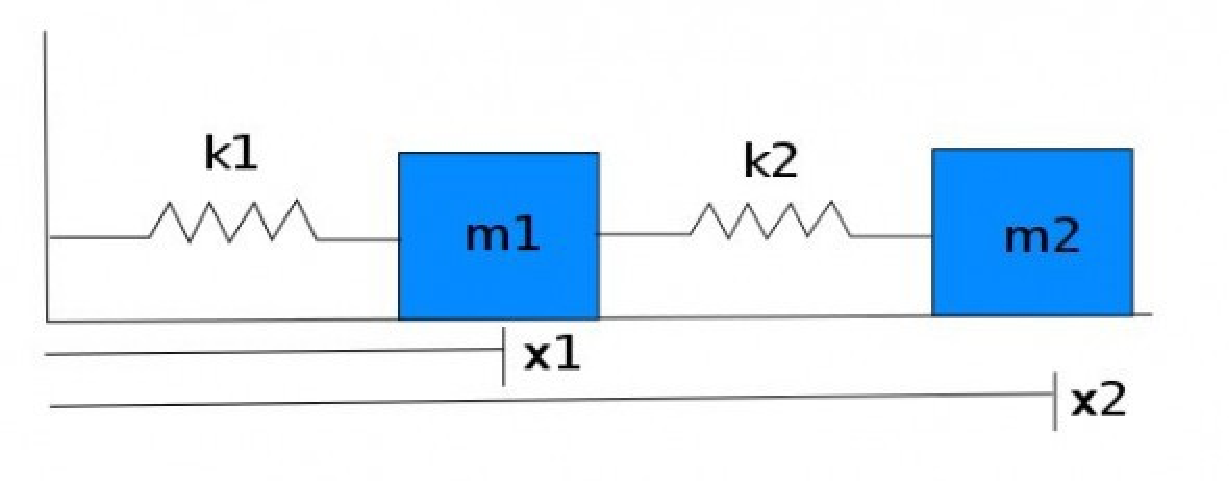
\includegraphics[width=0.6\columnwidth]{CoupledSpringMass}
%     \end{center}
    \begin{flalign*}
        m_1 x_1 '' &= -\underline{\hspace{0.5in}} x_1 + k_2 \underline{\hspace{0.5in}} \\
        m_2 x_2 '' &= -\underline{\hspace{0.5in}} \left( x_2 - x_1 \right)
    \end{flalign*}
    Once you have the system, write it as a matrix equation.
\end{problem}
\solution{
    \begin{flalign*}
        m_1 x_1 '' &= -k_1 x_1 + k_2 (x_2 - x_1) = -(k_1+k_2)x_1 + k_2 x_2 \\
        m_2 x_2 '' &= -k_2 \left( x_2 - x_1 \right) = k_2 x_1 - k_2 x_2
    \end{flalign*}
    \[ \frac{d^2 \bx}{dt^2} = \begin{pmatrix} -(k_1+k_2) & k_2 \\ k_2 & -k_2 \end{pmatrix}
    \bx \]
}

\begin{problem}
    The previous problem ended in a $2\times 2$ second order system.  Make an appropriate
    substitution and arrive at a $4\times 4$ first order system.  
\end{problem}
\solution{
Let $y_1 = x_1'$ and $y_2 = x_2'$.  Therefore,
\begin{flalign*}
    m_1 y_1' &= -(k_1+k_2)x_1 + k_2 x_2 \\
    x_1' &= y_1 \\
    m_2 y_2' &= k_2 x_1 - k_2 x_2\\
    x_2' &= y_2
\end{flalign*}
\[ \begin{pmatrix} y_1' \\ x_1' \\ y_2' \\ x_2' \end{pmatrix} = \begin{pmatrix} 0 &  -(k_1 +
        k_2) & 0 & k_2 \\
        1 & 0 & 0 & 0 \\
        0 & k_2 & 0 & -k_2 \\
        0 & 0 & 1 & 0 \end{pmatrix} \begin{pmatrix} y_1 \\ x_1 \\ y_2 \\ x_2 \end{pmatrix}
\]
}


% \begin{problem}
%     \begin{itemize}
%             \input{ClickerQuestions/DEQ.10.18.070}
%     \end{itemize}
% \end{problem}



\section{The Eigenvalue Method for Linear Systems}
Now let's interweave the idea of eigenvalues in with systems of differential equations. As
we already know, the eigenvalues and eigenvectors of a matrix $A$ tell us the underlying
structure of the matrix.  In some sense they are the DNA of the matrix.  In the cases that
we investigate here the eigen-structure of $A$ will tell us about the solution curves of
the linear first order differential equation.

\begin{thm}\label{thm:eigen_ode}
    Let $\lambda$ be an eigenvalue of the matrix $A$ for the first
    order linear system 
    \[ \frac{d\bx}{dt} = A \bx. \]
    If $\bv$ is an eigenvector associated with eigenvalue $\lambda$ then 
    \[ \bx(t) = \bv e^{\lambda t} \]
    is a nontrivial solution of the system.
\end{thm}
\begin{proof}
    Let $A$ be a real square matrix and let $\bv$ and $\lambda$ be an eigen-pair for $A$.
    To check that $\bx = \bv e^{\lambda t}$ is a solution to the differential equation
    $\bx' = A\bx$ we substitute $\bx$ in on both sides and check.

    On the left-hand side of the differential equation we get
    \begin{flalign*}
        \frac{d\bx}{dt} = \frac{d}{dt} \left( \bv e^{\lambda t} \right) 
        = \bv \frac{d}{dt} \left( e^{\lambda t} \right) 
        = \bv \left( \lambda e^{\lambda t} \right) 
        = \lambda e^{\lambda t} \bv.
    \end{flalign*}
    On the right-hand side of the differential equation we get
    \begin{flalign*}
        A\bx = A \left( \bv e^{\lambda t} \right) 
        = e^{\lambda t} A \bv 
        = e^{\lambda t} \left( \lambda \bv \right) 
        = \lambda e^{\lambda t} \bv \quad \checkmark.
    \end{flalign*}
\end{proof}

\begin{thm}
    If $\bv_1, \bv_2, \dots, \bv_k$ are unique solutions to the first
    order linear system of equations
    $\bx'=A\bx$ then a linear combination 
    \[ \bv = \sum_{j=1}^k c_j \bv_j \]
    is also a solution of $\bx' = A \bx$.
\end{thm}
\begin{proof}
    Since the differential equation is linear we know that a linear combination of
    solutions is also a solution.  
\end{proof}

\begin{thm}
    If the matrix $A$ has eigenvectors $\bv_1, \bv_2, \ldots, \bv_n$ and associated
    eigenvectors $\lambda_1, \lambda_2, \ldots, \lambda_n$ then the general solution to
    the differential equation $\bx' = A \bx$ is
    \[ \bx(t) = \underline{\hspace{2in}} \]
\end{thm}
\begin{proof}
    (Fill in the blank above and prove the theorem)
\end{proof}
\solution{
    \[ \bx(t) =c_1 \bv_1 e^{\lambda_1 t} +c_2 \bv_2 e^{\lambda_2 t} + \cdots +c_k \bv_k
    e^{\lambda_k t} \]
    This follows immediately from the previous two theorems.
}

% \begin{problem}
%     Considering the previous two theorems, if
%     \[ \frac{d\bx}{dt} = A \bx \]
%     then what is the solution to the system?
% \end{problem}

\begin{problem}
    Solve the following linear system of differential equations.
    \begin{flalign*}
        x_1' &= 4x_1 - x_2 \\
        x_2' &= 2x_1 + x_2
    \end{flalign*}
    with initial conditions $x_1(0) = 1$ and $x_2(0) = 3$. Complete the problem by giving a plots
    $x_1$ vs $t$, $x_2$ vs $t$, and $x_2$ vs $x_1$.  Use technology to find the
    eigen-structure of the resulting matrix and to create the plots.
\end{problem}
\solution{
First write the system as a matrix equation $\bx' = A \bx$:
\[ \bx' = \begin{pmatrix} 4 & -1 \\ 2 & 1 \end{pmatrix} \bx. \]
Now observe that the eigen-pairs of $A$ are
\[ \bv_1 = \begin{pmatrix} 1\\2 \end{pmatrix} \text{ with } \lambda_1 = 2 \quad \text{and}
\quad \bv_2 = \begin{pmatrix}1\\1\end{pmatrix} \text{ with } \lambda_2 = 3. \]
Hence, the solution to the differential equation is
\[ \bx(t) = c_1 e^{2t} \begin{pmatrix} 1 \\ 2\end{pmatrix} + c_2 e^{3t} \begin{pmatrix} 1
    \\ 1 \end{pmatrix}. \]
To find the values of the constants we need to solve the system
\[ \begin{pmatrix} 1\\3\end{pmatrix} = c_1 \begin{pmatrix}1\\2\end{pmatrix} + c_2
\begin{pmatrix}1\\1\end{pmatrix}. \]
Augmenting and row reducing gives
\[ \left( \begin{array}{cc|c} 1&1&1\\2&1&3\end{array} \right) \to \left(
\begin{array}{cc|c} 1 & 1 & 1 \\ 0 & -1 & 1 \end{array} \right) \to \left(
\begin{array}{cc|c} 1 & 0 & 2 \\ 0 & 1 & -1 \end{array} \right). \]
so $c_1 = 2$ and $c_2 = -1$ and the full solution is
\[ \bx(t) = 2 e^{2t} \begin{pmatrix} 1 \\ 2\end{pmatrix} - e^{3t} \begin{pmatrix} 1
    \\ 1 \end{pmatrix}. \]

\begin{center}
    \begin{tikzpicture}
        \begin{axis}[axis lines=center, domain=0:1.5, xmin=0, xmax=1.5, grid]
            \addplot[smooth, very thick, blue] {2*exp(2*x) - exp(3*x)};
            \addplot[smooth, very thick, red] {4*exp(2*x) - exp(3*x)};
        \end{axis}
    \end{tikzpicture}
\end{center}
}

% \begin{problem}
%     \begin{itemize}
%             \input{ClickerQuestions/DEQ.10.20.030}
%     \end{itemize}
% \end{problem}


\begin{problem}
    Since we know that both $x_1=x_2=e^{3t}$ and $x_1=e^{-t}, x_2=-e^{-t}$ are solutions
    to the system 
    \begin{flalign*} 
        x_1' & =  x_1  +2x_2 \\ x_2' & = & 2x_1  + x_2 \\
    \end{flalign*} 
    Which of the following are also solutions?
\begin{enumerate}
    \item[(a)] 
\begin{flalign*}
    x_1 & =  3e^{3t}-e^{-t} \\
    x_2 & =  3e^{3t}+e^{-t} \\
  \end{flalign*} 
\item[(b)] 
\begin{flalign*}
    x_1 & =  -e^{3t}-e^{-t} \\
    x_2 & =  -e^{3t}+e^{-t} \\
  \end{flalign*} 

\item[(c)] 
\begin{flalign*}
     x_1 & =  2e^{3t}+4e^{-t} \\
    x_2 & = -4e^{-t}+2e^{3t} \\
  \end{flalign*} 

\item[(d)] 
\begin{flalign*}
    x_1 & =  0 \\
    x_2 & =  0 \\
\end{flalign*} 

\item[(e)] None of the above

\item[(f)] All of the above.

\end{enumerate}


\end{problem}
% \begin{problem}
%     \begin{itemize}
%             \input{ClickerQuestions/DEQ.10.20.040}
%     \end{itemize}
% \end{problem}



\begin{problem}
    Consider the system of differential equations,

\[
y'(t) = \left( 
\begin{array}{ccc}
14 & 0 & -4 \\
2 & 13 & -8 \\
-3 & 0 & 25 \\
\end{array}
\right) y(t)
\].

Which of the following functions solve this system?
\begin{enumerate}
    \item[(a)]
        $y(t) = \left( \begin{array}{c} 1 \\ 0 \\ 3 \\ \end{array} \right) e^{-4 t}$
    \item[(b)]
        $y(t) = \left( \begin{array}{c} 1 \\ 3 \\ 2 \\ \end{array} \right) e^{6 t}$
    \item[(c)]
        $y(t) = \left( \begin{array}{c} 4 \\ 0 \\ 1 \\ \end{array} \right) e^{13 t}$
    \item[(d)] None of the above
    \item[(e)] All of the above.
\end{enumerate}

\end{problem}
% \begin{problem}
%     \begin{itemize}
%             \input{ClickerQuestions/DEQ.10.20.050}
%     \end{itemize}
% \end{problem}

% \begin{problem}
%     \begin{itemize}
%             \input{ClickerQuestions/DEQ.10.22.100}
%     \end{itemize}
% \end{problem}

\begin{problem}\label{prob:linear_fighting}
    Two forces are fighting one another. Let $x$ and $y$ be the number of soldiers in each
    force and let $a$ and $b$ be the offensive fighting capacities of $x$ and $y$ respectively.
    Assume that forces are lost only to combat, and no reinforcements are brought in.
    \begin{enumerate}
        \item[(a)] Write a system of differential equations that models this scenario.
            Write the system as a matrix equation.
        \item[(b)] Solve the system using the eigenvalue method using sensible initial
            conditions and values for $a$ and $b$.
        \item[(c)] Determine values of $a$ and $b$ for which army $x$ wins and for which
            army $y$ wins.
    \end{enumerate}
\end{problem}


\begin{problem}\label{prob:linear_fighting_nonhom}
    In Problem \ref{prob:linear_fighting} we built a model that might be really good for
    hand-to-hand combat.  Let's tweak this model.
    \begin{enumerate}
        \item[(a)] Modify the model from Problem \ref{prob:linear_fighting} to allow each
            army to get a constant number of recruits each day (assume time is measured in
            days).
        \item[(b)] Propose a solution technique for this model and implement it.
        \item[(c)] Propose a way to find a steady state solution to your model (if it
            exists) and implement your idea.
    \end{enumerate}
\end{problem}

% \begin{problem}
%     \begin{itemize}
%             \input{ClickerQuestions/DEQ.10.19.010}
%     \end{itemize}
% \end{problem}

In a linear system where there is a constant non-homogeneity we need to modify our solution
technique.  Consider the system of differential equations
\begin{flalign}
    \bx'(t) = A \bx + \bb
    \label{eqn:nonhomog_linear_system}
\end{flalign}
where $\bx$ is a vector of functions, $A$ is a real matrix, and $\bb$ is a vector of
constants.  Problem \ref{prob:linear_fighting_nonhom} should result in a model of this
type and in that problem you proposed a solution technique and a method for finding the
steady-state solution.  Now let's summarize these techniques.
\begin{technique}
    Let $\bx$ be an $n\times n$ vector of single variable functions, let $A$ be an $n\times n$ real matrix, and let
    $\bb$ be an $n \times n$ real vector.  Consider the system of $n$ differential
    equations
    \[ \bx' = A \bx + \bb \]
    with initial conditions $\bx(0) = \bx_0$. Observe that this is a non-homogeneous
    differential equation with a constant non-homogeneity.  The general solution
    to the differential equation is
    \[ \bx(t) = \underline{\hspace{2in}} \]
    where \ldots (complete the technique)
\end{technique}
\solution{
    \[ \bx(t) = \sum_{j=1}^n c_j \left( \bv_j e^{\lambda_j t} \right) + \bw \]
    where $\bw$ is the steady state vector resulting from solving the equation $A \bw +
    \bb = \bo$ and the constants arise from the equation $\bx_0 - \bw = \sum_{j=1}^n c_j \bv_j$
}

\begin{problem}
    Consider the linear system of differential equations given by
    \[ \begin{pmatrix} x' \\ y' \end{pmatrix} = \begin{pmatrix} -3 & 1 \\ 0 & -3
        \end{pmatrix} \begin{pmatrix} x \\ y \end{pmatrix} + \begin{pmatrix} 3 \\ 6
    \end{pmatrix} \]
    with initial conditions $x(0) = 1$ and $y(0) = 0$.  Solve the system of equations,
    generate a plot of the solution, and find the steady state (if it exists).
\end{problem}

\begin{problem}
    Solve the second order differential equation $y'' + 4y' + 3y = 2$ by converting to a
    first order system.  Find the equilibrium if it exists.
\end{problem}
\solution{
Partial solution:\\
Let $x = y'$ and we can rewrite as
\begin{flalign*}
    x' &= -4y + 3x + 2 \\
    y' &= x
\end{flalign*}
which can be rewritten as 
    \[ \begin{pmatrix} x' \\ y' \end{pmatrix} = \begin{pmatrix} 3 & -4 \\ 1 & 0
        \end{pmatrix} \begin{pmatrix} x \\ y \end{pmatrix} + \begin{pmatrix} 2 \\ 0
    \end{pmatrix} \]
    The equilibrium can be found by solving
    \[ \begin{pmatrix} 0 \\ 0 \end{pmatrix} = \begin{pmatrix} 3 & -4 \\ 1 & 0
        \end{pmatrix} \begin{pmatrix} x \\ y \end{pmatrix} + \begin{pmatrix} 2 \\ 0
    \end{pmatrix} \]
}




\section{The Matrix Exponential}
Recall that if we are solving the first order linear homogeoneous differential equation
$x' = rx$ we know (from separation of variables) that the solution is $x(t) = x_0 e^{rt}$.
This is one of the simplest ordinary differential equation that there is!  In this chapter we
have encountered linear systems of differential equations that have a very similar form:
\begin{flalign}
    \bx' = A \bx
    \label{eqn:linear_system_matrix_eqn}
\end{flalign}
where $\bx$ this time is a vector of functions and $A$ is a matrix of values.  More
clearly, if $A$ is an $n \times n$ real matrix then a linear system of differential
equations can be written as
\[ \begin{pmatrix} x_1'(t) \\ x_2'(t) \\ \vdots \\ x_n'(t) \end{pmatrix} = \begin{pmatrix}
        a_{11} & a_{12} & \cdots & a_{1n} \\
        a_{21} & a_{22} & \cdots & a_{2n} \\
    \vdots & \vdots & \ddots & \vdots \\
a_{n1} & a_{n2} & \cdots & a_{nn} \end{pmatrix} \begin{pmatrix} x_1(t) \\ x_2(t) \\ \vdots
\\ x_n(t) \end{pmatrix}. \]
It stands
to reason that the solution to \eqref{eqn:linear_system_matrix_eqn} should be the same, or
at least have the same form, as the solution to the simple differential equation $x' =
rx$.  Hence we conjecture that the solution to \eqref{eqn:linear_system_matrix_eqn} is
\begin{flalign}
    \bx = e^{A t} \bx_0
    \label{eqn:linear_system_matrix_eqn_soln}
\end{flalign}
where $\bx_0$ is the vector of initial conditions. \ldots but wait!  What is $e^{At}$?
That's right, we have a matrix in the exponent of an exponential function!

To understand the matrix exponential we first start by recalling the Taylor series of the
exponential function
\[ e^x = 1 + x + \frac{x^2}{2} + \frac{x^3}{3!} + \frac{x^4}{4!} + \cdots. \]
If instead we examine the function $f(x) = e^{ax}$ where $a \in \mathbb{R}$ then it is
easy to see that
\[ e^{ax} = 1 + ax + a^2 \frac{x^2}{2} + a^3 \frac{x^3}{3!} + a^4 \frac{x^4}{4!} + \cdots.
\]

If we use the Taylor series as the definition of the exponential function then a natural
definition for the matrix exponential is as follows.
\begin{definition}[Matrix Exponential]
    Let $A$ be a square matrix and $t$ be a real variable.  The matrix exponential
    $e^{At}$ is defined as
    \begin{flalign}
        e^{At} = I + At + A^2 \frac{t^2}{2} + A^3 \frac{t^3}{3!} + A^4 \frac{t^4}{4!} +
        \cdots.
        \label{eqn:matrix_exponential_Taylor}
    \end{flalign}
\end{definition}
Recall that if $A$ has a complete collection of eigenvalues and eigenvectors
then we can find matrices $P$ and $D$ such that $A = PDP^{-1}$.  Therefore the definition
of the matrix exponential can be rewritten as
\begin{flalign}
    \notag e^{At} &= I + PDP^{-1}t + PD^2P^{-1} \frac{t^2}{2} + PD^3P^{-1} \frac{t^3}{3!} +
    PD^4P^{-1} \frac{t^4}{4!} + \cdots \\
    &= P \left(  I + Dt + D^2 \frac{t^2}{2} + D^3 \frac{t^3}{3!} + D^4 \frac{t^4}{4!} +
    \cdots \right) P^{-1} 
    \label{eqn:matrix_exponential_Taylor_Eigen}
\end{flalign}


Using either \eqref{eqn:matrix_exponential_Taylor} or
\eqref{eqn:matrix_exponential_Taylor_Eigen} we now have a way to find the analytic
solution to a linear homogeneous system of differential equations of the form $\bx' = A
\bx$.  

\begin{thm}\label{thm:system_soln_matrix_exp}
    If $\bx$ is a vector of functions and $A$ is a real square matrix then the solution to
    the differential equation $\bx' = A \bx$ is
    \[ \bx(t) = e^{At} \bx_0. \]
\end{thm}

The computation of the matrix exponential in Theorem \ref{thm:system_soln_matrix_exp} is
potentially really obnoxious by hand, but thankfully there are built-in tools for
performing the computation in the most scientific computing software.  For example, in
MATLAB you can use the command \mcode{expm(A)} to find the matrix exponential of the matrix
$A$.

\begin{example}
    Use the matrix exponential to solve the system of differential equations 
    \[ \bx'(t) = \begin{pmatrix} 2 & 0 \\ 1 & 2 \end{pmatrix} \bx(t) \quad \text{with}
        \quad \begin{pmatrix} x_1(0) \\ x_2(0) \end{pmatrix} = \begin{pmatrix} 2 \\ -3
    \end{pmatrix} \]
    {\bf Solution:} The following MATLAB code finds the matrix exponential
\begin{lstlisting}
clear; clc;
syms t
A = [2 , 0 ; 1 , 2];
x0 = [2;-3];
x = expm(A*t) * x0   % this is the solution to the system of ODEs
\end{lstlisting}
    which results in the solution 
    \[ \begin{pmatrix} x_1(t) \\ x_2(t) \end{pmatrix} = \begin{pmatrix} e^{2t} & 0 \\
        te^{2t} & e^{2t} \end{pmatrix} \begin{pmatrix} 2 \\ -3 \end{pmatrix}. \]
    pulling this out of matrix form we have
    \[ x_1(t) = 2e^{2t} \quad \text{and} \quad x_2(t) = 2te^{2t} - 3e^{2t}. \]
    Finally we can plot the solution with the following code.
\begin{lstlisting}
tmax = 1;
ezplot(x(1),[0,tmax])
hold on
ezplot(x(2),[0,tmax])
axis([0,1,-10,10])
\end{lstlisting}
\end{example}
Hint: You can use
the command \mcode{latex(simplify(x))} to take your symbolic answer for $\bx(t)$ from MATLAB and get it into \LaTeX.

The following two problems give you a chance to practice using the matrix exponential to
solve applied systems of differential equations problems.  Have fun!!

\begin{problem}
    Tank \#1 is connected to Tank \#2 by two separate pipes.  Pure water is flowing
    into Tank \#1 at a rate of 2 gallons per minute.  Tank \#1 is initially filled with 50
    gallons of water with 5 pounds of salt dissolved in it.  Tank \#2 contains 40 gallons
    of water with 1 pound of salt dissolved in it.  Solution flows from Tank \#1 to Tank
    \#2 at a rate of 3 gallons per minute and from Tank \#2 to Tank \#1 and at a rate of 1
    gallon per minute.  Thoroughly mixed solution is also being drained from Tank \#2 at a
    rate of 2 gallons per minute.  Let $x(t)$ be the amount of salt in Tank \#1 and let
    $y(t)$ be the amount of salt in Tank \#2 at time $t$.  
    \begin{enumerate}
        \item[(a)] Write the linear system of differential equations that models this
            scenario. Be sure to include your initial conditions (it may help to draw a
            picture first).
        \item[(b)] Solve the system of differential equations using the matrix
            exponential.  Clearly write your answer in matrix and  vector form.
        \item[(c)] Solve the system again using the eigenvalue method.  Clearly write your
            answer showing how the eigenvalues and eigenvectors play a role in the
            solution.
        \item[(d)] Make a plot showing how the two concentrations evolve over 100 minutes.
    \end{enumerate}
\end{problem}




\begin{problem}
    You are given a mechanical system with three springs $A$, $B$, and $C$ and two
    objects $F$ and $G$ each of mass $M$.  Springs $A$ and $C$ have spring constant
    $k$ and spring $B$ has spring constant $2k$.  Spring $A$ is attached to a wall on
    the left and spring $C$ is attached to a wall on the right. Let $x_1(t)$ be the
    position of $F$ from it's equilibrium ($x_1=0$ indicates that $F$ is at
    equilibrium), and let $x_2(t)$ be the position of $G$ from it's equilibrium.  See
    Figure \ref{fig:double_spring_mass}.
    \begin{figure}[ht!]
        \begin{center}
            \begin{tikzpicture}
                \tikzstyle{ground}=[fill,pattern=north east lines,draw=none,minimum width=0.3,minimum height=0.6]
                \tikzstyle{sky}=[fill,pattern=north east lines,draw=none,minimum width=0.3,minimum height=0.6]

                \node (wall1) [ground, minimum height=2cm] {};
                \draw (wall1.north east) -- (wall1.south east);
                \node [draw,minimum width=0.5cm,minimum height=0.5cm] (massF) at (3,0) {$F$};
                \node [draw,minimum width=0.5cm,minimum height=0.5cm] (massG) at (5,0) {$G$};
                \node (rightend) at (8,0) [sky,minimum height=2cm] {};
                \draw (rightend.south west) -- (rightend.north west);
                \node (fix) at (0,0) {};
                \draw [
                    snake=coil,
                    segment amplitude=5pt,
                    segment length=5pt
                ] (wall1.east) -- (massF); 
                \draw [
                    snake=coil,
                    segment amplitude=5pt,
                    segment length=5pt
                ] (massF.east) -- (massG.west); 
                \draw [
                    snake=coil,
                    segment amplitude=5pt,
                    segment length=5pt
                ] (massG.east) -- (rightend.west); 
                \draw [
                    thick,
                    decoration={
                        brace,
                        mirror,
                        raise=0.5cm
                    },
                    decorate
                ] (wall1.east) -- (massF) 
                node [pos=0.5,anchor=north,yshift=-0.55cm] {$A$}; 
                \draw [
                    thick,
                    decoration={
                        brace,
                        mirror,
                        raise=0.5cm
                    },
                    decorate
                ] (massF.east) -- (massG.west) 
                node [pos=0.5,anchor=north,yshift=-0.55cm] {$B$}; 
                \draw [
                    thick,
                    decoration={
                        brace,
                        mirror,
                        raise=0.5cm
                    },
                    decorate
                ] (massG.east) -- (rightend) 
                node [pos=0.5,anchor=north,yshift=-0.55cm] {$C$}; 
            \end{tikzpicture}
        \end{center}
        \caption{Double spring mass system}
        \label{fig:double_spring_mass}
    \end{figure}
    
    Initial conditions: Assume that we move mass $F$ exactly 1 unit to the
            left and let it go.  This means that $x_1(0) = -1$ and $x_3(0) = x_1'(0) = 0$.
            If we initially hold mass $G$ fixed then $x_2(0)=x_4(0)=0$.    
    \begin{enumerate}
        \item[(a)] First we'll write the second order linear system of equations.  This system of
            equations is just a statement of Hooke's law for springs: $F = -kx$, where $k$ is
            the spring constant.  To help you get
            started you can use the skeleton below:
            \begin{flalign*}
                M x_1'' &= -k x_1 + \left( \text{some spring constant} \right) \left(
                \text{distance between $x_2$ and $x_1$}
                \right) \\
                M x_2'' &= -2k \left( x_2 - x_1 \right) - \left( \text{some spring constant}
                \right) x_2
            \end{flalign*}


        \item[(b)] To turn this into a first-order system we introduce two new variables: $x_3 =
            x_1'$ and $x_4 = x_2'$.  Write this system of differential equations \dots I'll
            get you started \dots
            \begin{flalign*}
                x_1' &= x_3 \\
                x_2' &= x_4 \\
                x_3' &= \text{ \dots } \\
                x_4' &=  \text{ \dots }
            \end{flalign*}
            Now write the system as a matrix equation of the form $\frac{d\bx}{dt} = A \bx$.

        \item[(c)] Solve the linear system of differential equations with the method of
            matrix exponentials.
        \item[(d)] Next solve the linear system of differential equations with the
            eigenvalue method. You {\it should} find that you have 4 purely imaginary
            eigenvalues (I'll wait while you let MATLAB find these for you \dots).  This
            means that you will have oscillations in your solutions. Why?
%         
% 
%         
%         Hence, if we let $\lambda_j = \alpha_j
%         i$ then $e^{\lambda_j t} = \cos(\alpha_j t) + i\sin(\alpha_j t)$ by Euler's
%         formula.  Therefore, the solution to the system of differential equations becomes
%         \begin{flalign*} \bx(t) &= \left( A_1 \cos(\alpha_1 t) + B_1 \sin(\alpha_1 t)
%             \right) \bv_1 \\
%             &\quad+\left( A_2 \cos(\alpha_2 t) + B_2 \sin(\alpha_2 t) \right) \bv_2 \\
%             &\quad+\left( A_3 \cos(\alpha_3 t) + B_3 \sin(\alpha_3 t) \right) \bv_3 \\
%             &\quad+\left( A_4 \cos(\alpha_4 t) + B_4 \sin(\alpha_4 t) \right) \bv_4.
%         \end{flalign*}
%         You should have values of $\alpha_1, \alpha_2, \alpha_3,$ and $\alpha_4$ as well
%         as the eigenvectors $\bv_1, \bv_2, \bv_3$, and $\bv_4$.

        \item[(e)] Plot your solutions.
    \end{enumerate}
\end{problem}


\section{Complex Eigenvalues}
In this brief section we consider the case where the eigenvalues of the coefficient matrix
in a linear system are complex.  If $\bx' = A \bx$ and $A$ has complex eigenvalues
$\lambda = \alpha \pm \beta i$ then the solution to the system is
\[ \bx(t) = C_1 e^{\lambda_1 t} \bv_1 + C_2 e^{\lambda_2 t} \bv_2 = e^{\alpha t} \left(
C_1 e^{\beta i t} \bv_1 + C_2 e^{-\beta i t} \bv_2 \right). \]
If we use Euler's formula for the complex exponentials the solution becomes
\[ \bx(t) = e^{\alpha t} \left( C_1 \left( \cos(\beta t) + i\sin(\beta t) \right) \bv_1 +
C_2 \left( \cos(\beta t) - i\sin(\beta t) \right) \bv_2 \right). \]
Now if we gather the trigonometric functions the solution can be written as
\begin{flalign} \bx(t) = e^{\alpha t} \left[ \left( C_1 \bv_1 + C_2 \bv_2 \right) \cos(\beta t) +
\left( C_1 i \bv_1 - C_2 i \bv_2 \right) \sin(\beta t)
\right].\label{eqn:linear_system_oscillations}
\end{flalign}
Form the initial conditions we know that $\bx(0) = C_1 \bv_1 + C_2 \bv_2$ and once we have
calculated $C_1$ and $C_2$ it is straight forward to find the vectors multiplying the
cosine and sine terms in the solution.

\begin{example}\label{ex:linear_system_oscillation}
    Solve the system of differential equations 
    \[ \bx'(t) = \begin{pmatrix} -2 & -2 \\ 2 & -2 \end{pmatrix} \bx(t) \]
    with initial condition $\bx(0) = \begin{pmatrix} 3 \\ -3 \end{pmatrix}$. \\
    {\bf Solution:} We first need to find the eigenvalues and eigenvectors of the
    coefficient matrix, $A$.  
    \[ \bv_1 = \begin{pmatrix} -i \\ -1 \end{pmatrix} \quad \text{with} \quad \lambda_1 =
    -2 + 2i \]
    \[ \bv_2 = \begin{pmatrix} i \\ -1 \end{pmatrix} \quad \text{with} \quad \lambda_2 =
    -2 - 2i \]
    Solve the system of equation $\begin{pmatrix} \bv_1 \, \bv_2 \end{pmatrix}
    \begin{pmatrix} C_1 \\ C_2 \end{pmatrix} = \bx(0)$ to get $C_1 = \frac{3}{2} +
    \frac{3}{2} i$ and $C_2 = \frac{3}{2} - \frac{3}{2} i$ (the actual computation is left
    to the reader). 
    Hence,
    \[ C_1 \bv_1 + C_2 \bv_2 = \left( \frac{3}{2} + \frac{3}{2} i \right) \begin{pmatrix}
        -i \\ -1 \end{pmatrix} + \left( \frac{3}{2} - \frac{3}{2}i \right) \begin{pmatrix}
    i \\ -1 \end{pmatrix} = \cdots = \begin{pmatrix} 3 \\ -3 \end{pmatrix}  \]
    and
    \[ C_1i \bv_1 - C_2i \bv_2 = \left( \frac{3}{2} + \frac{3}{2} i \right)i \begin{pmatrix}
        -i \\ -1 \end{pmatrix} - \left( \frac{3}{2} - \frac{3}{2}i \right)i \begin{pmatrix}
    i \\ -1 \end{pmatrix} = \cdots = \begin{pmatrix} 3 \\ 3 \end{pmatrix}  \]
    Now we can substitute into \eqref{eqn:linear_system_oscillations} to get the complete
    solution
    \[ \bx(t) = e^{-2t} \left( \cos(2t) \begin{pmatrix} 3 \\ -3 \end{pmatrix} + \sin(2t)
    \begin{pmatrix} -3 \\ 3 \end{pmatrix} \right) = \begin{pmatrix} e^{-2t} \left( 3
        \cos(2t) + 3 \sin(2t)
    \right) \\ e^{-2t} \left( -3\cos(2t) + 3\sin(2t) \right) \end{pmatrix}. \]
    The solutions to the system are shown in Figure \ref{fig:linear_system_oscillation}
\end{example}

\begin{figure}
    \begin{center}
        \begin{tikzpicture}
            \begin{axis}[axis lines=center, domain=0:3, xmin=0, xmax=3, ymin=-3.1, ymax=3.1,
                xlabel={$t$}]
                \addplot[blue, very thick, samples=100] {exp(-2*x)*(3*cos(2*deg(x)) + 3*sin(2*deg(x)))};
                \addlegendentry{$x(t)$};
                \addplot[red, very thick, samples=100] {exp(-2*x)*(-3*cos(2*deg(x)) + 3*sin(2*deg(x)))};
                \addlegendentry{$y(t)$};
            \end{axis}
        \end{tikzpicture}
    \end{center}
    \caption{Solution curves for Example \ref{ex:linear_system_oscillation}}
    \label{fig:linear_system_oscillation}
\end{figure}


\section{Additional Exercises}

\setcounter{chapter}{8}
\chapter{Nonlinear Systems of Differential Equations}
The world is non-linear!  Well shoot. It might seem that this means that for {\it real}
problems we can't use anything that we've done so far.   Wrong!  There are plenty of
things that we can do with nonlinear problems.  For the most part we will rely on a basic
premise from Calculus: up close, a nonlinear function looks linear. You did this back in
calculus when you found tangent lines and tangent planes but now we're going to do the
same for matrices and nonlinear differential equations.  For most of the problems in this
chapter it will be helpful to have MATLAB up so you can plot phase planes and analyze
equilibria graphically.

\section{Modeling a Nonlinear System}
\begin{problem}
    We're going to try a social experiment.  
    \begin{enumerate}
        \item[(a)] Everyone in the class get a random number between 1 and 5. 
        \item[(b)] I'm sorry, but if your random number is ``1'' then you just got infected
            with the horribly contagious disease ODEbola.  Raise your hand if you are
            infected.
        \item[(c)] For the next 15 seconds everyone needs to walk aimlessly around the
            classroom (move the tables out of the way and don't be afraid to bump into
            each other).  This step is supposed to simulate {\it homogeneous mixing} so
            \ldots mix homogeneously!
        \item[(d)] At the end of the 15 seconds stop and stand still.  Reach your arms
            out.  If someone within arm's reach is infected with ODEbola then you now are
            too!  Raise your hand if you are infected.
        \item[(e)] Repeat steps (c) and (d) again. At the end of every step 10\% of the
            infected people that are infected will recover and are removed from the
            experiment.  Keep track of the number of
            people that are infected and recovered at each step.  Run the experiment for
            several iterations
    \end{enumerate}
\end{problem}

\begin{problem}\label{prob:SIR_outbreak_simulation}
    Watch the video \href{https://youtu.be/NSNWDUXN2p4}{https://youtu.be/NSNWDUXN2p4} to
    see a simulation where a 150 person population has an outbreak and the virus is spread
    via close proximity contact.  Notice, in particular,
    the homogeneous mixing.
\end{problem}

\begin{challenge}
    Write computer code to produce a simulation similar to what you see in Problem
    \ref{prob:SIR_outbreak_simulation}.
\end{challenge}

\begin{problem}
    In the previous problems there were three distinct populations: Susceptible ($S$),
    Infected ($I$), and Recovered ($R$).  Write a system of differential equations for the
    experiment that we ran and remember to keep in mind that we were homogeneously mixing
    the population the entire time. Think very carefully about how a susceptible person is
    actually infected.
    \begin{flalign*}
        \frac{dS}{dt}&= \underline{\hspace{2in}} \quad \text{with} \quad S(0) =
        \underline{\hspace{1in}} \\
        \frac{dI}{dt}&= \underline{\hspace{2in}} \quad \text{with} \quad I(0) = 
        \underline{\hspace{1in}} \\
        \frac{dR}{dt}&= \underline{\hspace{2in}}  \quad \text{with} \quad R(0) = 
        \underline{\hspace{1in}} \\
    \end{flalign*}
\end{problem}
\solution{
    The system should be a standard SIR model where the recovered people can also get
    infected.
    \begin{flalign*}
        S' &= -\alpha SI \\
        I' &= \alpha SI - \beta I \\
        R' &= \beta I
    \end{flalign*}
    where $\alpha$ is a parameter related to the likelihood that someone will get infected
    (subject to the homogeneous mixing) and $\beta = 0.1$ is the recovery rate.
}


\begin{problem}
    Consider the system from the previous problem.
    \begin{enumerate}
%         \item[(a)] How did you take the homogeneous mixing into account?
        \item[(a)] Is the system linear or nonlinear?  Why?
        \item[(b)] What is the expected long-term behavior of this system?  Why?
    \end{enumerate}
\end{problem}


\section{Trace-Determinant Plane}
In this section we will briefly examine a technique for quickly determining
the behavior of 2D linear systems.  This will play a major role in our nonlinear systems
since each nonlinear system will eventually be linearized as we will see in a bit.  


Recall that if $\bv_1$ and $\bv_2$ are the eigenvectors of $A$ with eigenvalues
$\lambda_1$ and $\lambda_2$ then the solution to the first order linear system of
equations $\bx' = A \bx$ is
\[ \bx = c_1 e^{\lambda_1 t} \bv_1 + c_2 e^{\lambda_2 t} \bv_2 \]
where $\bx_0 = c_1 \bv_1 + c_2 \bv_2$.  Furthermore we observe that $\bx = \bo$ is an
equilibrium point of the system of differential equations.  Use these ideas to answer the
following questions.
\begin{problem}
    Consider the $2\times 2$ linear system of differential equations $\bx'=A\bx$.  In each
    of the following cases what is the expected behavior of the solution? The choices are:
    spirals in to the origin, spirals out from the origin, decays in to the origin,
    diverges out from the origin, decays toward the origin but then diverges out, or
    circles the origin.
            \begin{enumerate}
                \item If $\lambda_1 \le \lambda_2 < 0$ then near the origin the
                    solution \underline{\hspace{1in}}
                    \solution{decays in}
                \item If $\lambda_1 < 0 < \lambda_2$ then near the origin the
                    solution \underline{\hspace{1in}}
                    \solution{decays toward the origin but then divers out}
                \item If $\lambda_1 \ge \lambda_2 > 0$ then near the origin the
                    solution \underline{\hspace{1in}}
                    \solution{diverges out from the origin}
                \item If $\lambda_1, \lambda_2 = \alpha \pm \beta i \, (\alpha<0)$ then
                    near the origin the solution \underline{\hspace{1in}}
                    \solution{spirals in toward the origin}
                \item If $\lambda_1, \lambda_2 = \alpha \pm \beta i \, (\alpha>0)$ then
                    near the origin the solution \underline{\hspace{1in}}
                    \solution{spirals out from the origin}
                \item If $\lambda_1, \lambda_2 = \pm \beta i$ then near the origin
                    the solution \underline{\hspace{1in}}
                    \solution{circles the origin}
            \end{enumerate}
\end{problem}

\begin{problem}
    In the following plots the two eigenvectors for a matrix $A$ are plotted and the
    eigenvalues are given.  Sketch the trajectory of the solution in the $xy$-plane
    starting at the given points (use your answers from the previous problem to help).
    \begin{center}
        \begin{tikzpicture}
            \draw[very thick, <->, black] (-3,0) -- (3,0);
            \draw[very thick, <->, black] (0,-2.5) -- (0,2.5);
            \draw[very thick, red, ->, dashed] (0,0) -- (1,2) node[anchor=south
            west]{$\lambda_1 = -2$}; 
            \draw[very thick, blue, ->, dotted] (0,0) -- (-2,-1) node[anchor=north
            east]{$\lambda_2 = -0.25$}; 
            \draw[fill=black] (1.0,1.0) circle(0.075cm);
            \draw[fill=black] (-1,-1) circle(0.075cm);
            \draw[fill=black] (-1,1) circle(0.075cm);
            \draw[fill=black] (1,-1) circle(0.075cm);
        \end{tikzpicture}\hspace{0.4in}
        \begin{tikzpicture}
            \draw[very thick, <->, black] (-3,0) -- (3,0);
            \draw[very thick, <->, black] (0,-2.5) -- (0,2.5);
            \draw[very thick, red, ->, dashed] (0,0) -- (1,2) node[anchor=south
            west]{$\lambda_1 = 2$}; 
            \draw[very thick, blue, ->, dotted] (0,0) -- (-2,-1) node[anchor=north
            east]{$\lambda_2 = -0.25$}; 
            \draw[fill=black] (1.0,1.0) circle(0.075cm);
            \draw[fill=black] (-1,-1) circle(0.075cm);
            \draw[fill=black] (-1,1) circle(0.075cm);
            \draw[fill=black] (1,-1) circle(0.075cm);
        \end{tikzpicture}
    \end{center}
    \begin{center}
        \begin{tikzpicture}
            \draw[very thick, <->, black] (-3,0) -- (3,0);
            \draw[very thick, <->, black] (0,-2.5) -- (0,2.5);
            \draw[very thick, red, ->, dashed] (0,0) -- (1,2) node[anchor=south
            west]{$\lambda_1 = 2$}; 
            \draw[very thick, blue, ->, dotted] (0,0) -- (-2,-1) node[anchor=north
            east]{$\lambda_2 = 0.25$}; 
            \draw[fill=black] (1.0,1.0) circle(0.075cm);
            \draw[fill=black] (-1,-1) circle(0.075cm);
            \draw[fill=black] (-1,1) circle(0.075cm);
            \draw[fill=black] (1,-1) circle(0.075cm);
        \end{tikzpicture}\hspace{0.4in}
        \begin{tikzpicture}
            \draw[very thick, <->, black] (-3,0) -- (3,0);
            \draw[very thick, <->, black] (0,-2.5) -- (0,2.5);
            \draw[very thick, red, ->, dashed] (0,0) -- (1,2) node[anchor=south
            west]{$\lambda_1 = -2+i$}; 
            \draw[very thick, blue, ->, dotted] (0,0) -- (-2,-1) node[anchor=north
            east]{$\lambda_2 = -2-i$}; 
            \draw[fill=black] (1.0,1.0) circle(0.075cm);
            \draw[fill=black] (-1,-1) circle(0.075cm);
            \draw[fill=black] (-1,1) circle(0.075cm);
            \draw[fill=black] (1,-1) circle(0.075cm);
        \end{tikzpicture}
    \end{center}
    \begin{center}
        \begin{tikzpicture}
            \draw[very thick, <->, black] (-3,0) -- (3,0);
            \draw[very thick, <->, black] (0,-2.5) -- (0,2.5);
            \draw[very thick, red, ->, dashed] (0,0) -- (1,2) node[anchor=south
            west]{$\lambda_1 = 2+i$}; 
            \draw[very thick, blue, ->, dotted] (0,0) -- (-2,-1) node[anchor=north
            east]{$\lambda_2 = 2-i$}; 
            \draw[fill=black] (1.0,1.0) circle(0.075cm);
            \draw[fill=black] (-1,-1) circle(0.075cm);
            \draw[fill=black] (-1,1) circle(0.075cm);
            \draw[fill=black] (1,-1) circle(0.075cm);
        \end{tikzpicture}\hspace{0.4in}
        \begin{tikzpicture}
            \draw[very thick, <->, black] (-3,0) -- (3,0);
            \draw[very thick, <->, black] (0,-2.5) -- (0,2.5);
            \draw[very thick, red, ->, dashed] (0,0) -- (1,2) node[anchor=south
            west]{$\lambda_1 = i$}; 
            \draw[very thick, blue, ->, dotted] (0,0) -- (-2,-1) node[anchor=north
            east]{$\lambda_2 = -i$}; 
            \draw[fill=black] (1.0,1.0) circle(0.075cm);
            \draw[fill=black] (-1,-1) circle(0.075cm);
            \draw[fill=black] (-1,1) circle(0.075cm);
            \draw[fill=black] (1,-1) circle(0.075cm);
        \end{tikzpicture}
    \end{center}
\end{problem}

Now that we know the general behavior of all $2 \times 2$ systems based on the
eigen-structure let's get a faster way to make the determination.  That is, if we can
avoid actually finding the eigenvalues that might save some time.
\begin{problem}
    Let the $2 \times 2$ linear system $\bx' = A \bx$ be written as
    \[ \begin{pmatrix} x' \\ y' \end{pmatrix} = \begin{pmatrix} a & b \\ c & d
        \end{pmatrix} \begin{pmatrix} x \\ y \end{pmatrix} \]
    Your Tasks:
    \begin{enumerate}
        \item What is the equilibrium of this system presuming that $A^{-1}$ exists?
        \item Find the characteristic polynomial of the coefficient matrix
        \item Simplify the characteristic polynomial to fill in the blanks:
            \[ \lambda^2 + \underline{\hspace{0.5in}} \lambda + \underline{\hspace{0.5in}}
                = 0
                \]
            The blanks should be familiar features of the matrix.
    \end{enumerate}
\end{problem}
\solution{
    The solution to the system is $\bx = \bo$ since we solve $\bo = A
    \bx$ to find the equilibrium and if $A^{-1}$ exists then $\bx = \bo$.  

    The characteristic polynomial is:
$p(\lambda) = \lambda^2 - tr(A) \lambda + \det(A) $
}



\begin{problem}
    In the previous problems you found that the characteristic polynomial for a 2D linear
    system is $p(\lambda) = \lambda^2 - T \lambda + D$ where $T = \text{tr}(A)$ and $D=
    \det(A)$.  Solving for $\lambda$ we see that
    \[ \lambda = \frac{T \pm \sqrt{T^2 - 4 D}}{2}. \]
    Clearly the behavior of the eigenvalues depends on the quantity $T^2 - 4D$.  To
    visualize this we create the {\it trace-determinant} plane as seen in the figure
    immediately below.  Fill in the question marks in the figure with the type of behavior
    you expect to see for each region of the {\it trace-determinant} plane?

    To illustrate what we mean condsider the furthest right question mark.  In that
    question mark the determinant, $D$, is greater than zero, the trace, $T$, is greater
    than zero and $D < T^2 / 4$.  Hence $T^2 - 4D>0$ so we expect the behavior of the
    system to be a nodal source since both eigenvalues will be real and positive.

    Use the following words to fill in the question marks: nodal source, nodal sink,
    spiral source, spiral sink, center, and saddle.
\end{problem}
    \vspace{-0.1in}
        \begin{center}
            \begin{tikzpicture}
                \begin{axis}[xlabel={$T=tr(A)$},ylabel={$D=\det(A)$}, ymin=-0.5,
                        ymax=0.5, xmin=-2, xmax=2, xtick=\empty, ytick=\empty, legend pos=outer
                    north east]
                    \addplot[smooth,blue, very thick, domain=-2:2] {(1/4)*x^2};
                    \addlegendentry{$D = T^2/4$};
                    \addplot[smooth, black, thick] {0*x};
                    \draw[black,thick] (axis cs:0,-0.5) -- (axis cs:0,0.5);
                    \node at (axis cs:1.5,0.1) {?};
                    \node at (axis cs:-1.5,0.1) {?};
                    \node at (axis cs:-.5,0.25) {?};
                    \node at (axis cs:.5,0.25) {?};
                    \node at (axis cs:0,0.3) {?};
                    \node at (axis cs:0.5,-0.25) {?};
                    \node at (axis cs:-0.5,-0.25) {?};
                \end{axis}
            \end{tikzpicture}
        \end{center}

\solution{
        \begin{center}
            \begin{tikzpicture}
                \begin{axis}[xlabel={$T=tr(A)$},ylabel={$D=\det(A)$}, ymin=-0.5,
                        ymax=0.5, xmin=-2, xmax=2, xtick=\empty, ytick=\empty, legend pos=outer
                    north east]
                    \addplot[smooth,blue, very thick, domain=-2:2] {(1/4)*x^2};
                    \addlegendentry{$D = T^2/4$};
                    \addplot[smooth, black, thick] {0*x};
                    \draw[black,thick] (axis cs:0,-0.5) -- (axis cs:0,0.5);
                    \node at (axis cs:1.5,0.1) {\tiny{nodal source}};
                    \node at (axis cs:-1.5,0.1) {\tiny{nodal sink}};
                    \node at (axis cs:-.5,0.25) {\tiny{spiral sink}};
                    \node at (axis cs:.5,0.25) {\tiny{spiral source}};
                    \node at (axis cs:0,0.3) {\tiny{center}};
                    \node at (axis cs:0.5,-0.25) {\tiny{saddle}};
                    \node at (axis cs:-0.5,-0.25) {\tiny{saddle}};
                \end{axis}
            \end{tikzpicture}
        \end{center}
    }

% \begin{problem}
%     Modeling a bungee jumper is much like modeling a 1-dimensional spring mass system
%     except for the fact that
%     the air resistance plays a major role.  According to Newton's second law as well as
%     Hooke's law
%     \[ m x'' = -kx + F_{drag} \quad \text{where} \quad F_{drag} = -a x' \]
%     Hence, the model for the motion of the bungee jumper is
%     \[ mx'' + ax' + kx = 0 \]
%     Dividing by mass we get
%     \[ x'' + \alpha x' + \kappa x = 0 \]
%     Turn this into a system of differential equations with an appropriate substitution,
%     discuss equilibria and stability, and explore it graphically.
% \end{problem}
% \solution{This is a straight foward linear system
%     \[ \left\{ \begin{array}{ll} x' &= y \\ y' &= - \alpha y - \kappa x \end{array}
%     \right. \]
%     Equlibrium: $(0,0)$.  Stable.
%     \[ A = \begin{pmatrix} 1 & 0 \\ -\kappa & -\alpha \end{pmatrix} \]
%     so 
%     \[ \lambda_{1,2} = \frac{-\alpha \pm \sqrt{\alpha^2 - 4 \kappa}}{2} \]
%     The real part is negative so the equilibrium is stable.
% 
% }

Now we'll finally look at some nonlinear systems.
\begin{problem}\label{prob:competin_species}
    Suppose that $x$ and $y$ are the population of two distinct species that compete for the
    same resources. For example, two species of fish may compete for the same food in a
    lake or sheep and cattle competing for the same grazing land. We can model two
    competing species using the following system of first-order differential equations, 
    \begin{flalign*}
        x' &= 2x\left( 1-\frac{x}{2} \right) - xy \\
        y' &= 3y\left( 1-\frac{y}{3} \right) - 2xy.
    \end{flalign*}
    It is reasonably easy to show that the four equilibrium solutions are $(0,0)$,
    $(0,3)$, $(2,0)$, and $(1,1)$.  Use the \texttt{pplane} software (linked from Moodle)
    to analyze what happens near the equilibrium $(1,1)$.
\end{problem}


Now we'll build up the analytic tools necessary to analyze the competing species model in
problem \ref{prob:competin_species}.
\begin{definition}[Nullclines and Equilibria]
    The {\bf nullclines} for a linear system 
    \begin{flalign*}
        x'(t) &= f(x,y) \\
        y'(t) &= g(x,y)
    \end{flalign*}
    are the curves where $f(x,y)=0$ and $g(x,y)=0$.  When two nullclines intersect there
    is and equilibrium solution.
\end{definition}
\begin{problem}
    Use a graphing tool to sketch the nullclines of the system and use your graph to
    verify the location of the equilibrium points.
    \begin{flalign*}
        x' &= 2x\left( 1-\frac{x}{2} \right) - xy \\
        y' &= 3y\left( 1-\frac{y}{3} \right) - 2xy.
    \end{flalign*}
\end{problem}
\solution{
    The nullclines are $2x(1-x/2)-xy=0$ and $3y(1-y/3)-2xy = 0$.  In the first one we
    either have the vertical line $x=0$ or the line $y=2(1-x/2)$.  In the second one we
    either have the horizontal line $y=0$ of the line $2x = 3(1-y/3)$.  Plotting all four
    of these lines together we see that the intersections are $(0,0)$, $(0,3)$, $(2,0)$,
    and $(1,1)$.
}

\begin{definition}[Jacobian Matrix]
    Consider the system of equations
    \begin{flalign*}
        f(x,y) &= 0 \\
        g(x,y) &= 0.
    \end{flalign*}
    The {\bf Jacobian matrix} for this system is defined as
    \[ J(x,y) = \begin{pmatrix} f_x & f_y \\ g_x & g_y \end{pmatrix} \]
    where subscripts mean partial dervatives.
\end{definition}

\begin{problem}
    Find the Jacobian matrix $J(x,y)$ for the system 
    \begin{flalign*}
        x' &= 2x\left( 1-\frac{x}{2} \right) - xy = 2x - x^2 - xy \\
        y' &= 3y\left( 1-\frac{y}{3} \right) - 2xy = 3y - y^2 - 2xy.
    \end{flalign*}
\end{problem}
\solution{
    \[ J(x,y) = \begin{pmatrix} 2-2x-y & -x \\ -2y & 3-2y-2x \end{pmatrix} \]
}

The Jacobian describes the local linear behavior of the system near an equilibrium.  That
is to say that if we substitute the values $(x_*,y_*)$ from an equilibrium point into the Jacobian
then {\it near} the equilibrium point will behave like the linear system $\bx' =
J(x_*,y_*) \bx$ centered at the equilibrium.  

\begin{problem}
    Verify the behavior of the system 
    \begin{flalign*}
        x' &= 2x\left( 1-\frac{x}{2} \right) - xy \\
        y' &= 3y\left( 1-\frac{y}{3} \right) - 2xy
    \end{flalign*}
    near the equilibrium $(1,1)$ (you already discussed this in Problem
    \ref{prob:competin_species}).  Then use the Jacobian matrix to discuss the behavior of
    the system near the other three equilibria.
\end{problem}
\solution{
    At $(1,1)$ we have $J(1,1) = \begin{pmatrix} -1 & -1 \\ -2 & -1 \end{pmatrix}$.
        Observe that $\text{tr}(J(1,1)) = -2$ and $\det(J(1,1)) = 1 - 2 = -1$.  From the
        trace-determinant plane we should have a saddle near $(1,1)$.
}



\begin{technique}[Equilibria and Stability of Nonlinear Systems]
    Consider the nonlinear system of differential equations
    \begin{flalign*}
        x'(t) &= f(x,y) \\
        y'(t) &= g(x,y).
    \end{flalign*}
    To find and analyze the equilibria for the system:
    \begin{enumerate}
        \item Find the equilibria by setting \underline{\hspace{0.5in}} to zero and
            solving for $x$ and $y$.  It may be necessary to use technology to solve this
            system of nonlinear equations.
        \item Find the Jacobian matrix at each of the equilibrium points.
        \item Investigate the \underline{\hspace{0.5in}} for each Jacobian matrix.  Based
            on this investigate you can make a claim about local stability.
    \end{enumerate}
\end{technique}

\begin{example}
    Consider the system 
    \begin{flalign*}
        x'(t) &= x-3y+xy^2 \\
        y'(t) &=  2x-4y-x^2y.
    \end{flalign*}
    Find the nullclines, equilibria, the Jacobian, and classify the equilibrium solutions.
    \\ {\bf Solution:} \\
    The nullclines are the curves $f(x,y) = 0$ and $g(x,y) = 0$ called the $x$-nullcline
    and the $y$-nullcline respectively since if $f=0$ the $x$-variable stops changing and
    if $g=0$ the $y$-variable stops changing.  
    \begin{flalign*}
        \text{$x$-nullcline: } 0&= x-3y+xy^2\\
        \text{$y$-nullcline: } 0&= 2x - 4y - x^2y
    \end{flalign*}
    These are rather complicated curves in the $xy$-plane.

    Using a computer algebra system the approximate equilibria are $(-1.06, -0.41)$, $(1.06,
    0.41)$, and $(0,0)$ (along with a few imaginary equilibria).

    The Jacobian is $J(x,y) = \begin{pmatrix} 1+y^2 & -3 + 2xy \\ 2-2xy & -4-x^2
    \end{pmatrix}$ 
    and at $(0,0)$ we have $J(0,0) = \begin{pmatrix} 1 & -3 \\ 2 & -4 \end{pmatrix}$.  For
    this equilibrium point, $T(0,0) = -3$ and $D(0,0) = (-4) - (-6) = 2$.  Hence $T^2/4 =
    9/4 = 2.25 > D$ so according to the trace-determinant plane we much have a spiral
    sink at $(0,0)$.
\end{example}




\section{Applied Nonlinear Systems}
Let's get started with a nonlinear system.  This system will be familiar in a lot of ways
but we will added a small wrinkle: air resistance.





\begin{problem}
    Modeling a bungee jumper is much like modeling a 1-dimensional spring mass system
    except for the fact that
    the air resistance plays a major role.  According to Newton's second law as well as
    Hooke's law
    \[ m x'' = -kx + F_d \quad \text{where} \quad F_d = -a x' -b \left( x' \right)^2 \]
    Hence, the model for the motion of the bungee jumper is
    \[ mx'' + ax' + b\left( x' \right)^2 + ky = 0 \]
    Dividing by mass we get
    \[ x'' + \alpha x' + \beta \left( x' \right)^2 + \kappa x = 0 \]
    Turn this into a system of differential equations with an appropriate substitution,
    discuss equilibria and stability, and explore it graphically.
\end{problem}
\solution{
    Let $x'=y$ and get the following:
    \[ \left\{ \begin{array}{ll} x'&= y \\ y' &= -\alpha y - \beta y^2 - \kappa x
    \end{array} \right. \]
    This is a nonlinear system!!

    Equlibria: Set $x'=y'=0$
    \[ \left\{ \begin{array}{ll} 0&= y \\ 0 &= -\alpha y - \beta y^2 - \kappa x
    \end{array} \right. \]
    Therefore, $x=y=0$ is the equilibrium.

    Local stability: Find the Jacobian:
    \[ J(x,y) = \begin{pmatrix} f_x & f_y \\ g_x & g_y \end{pmatrix} = \begin{pmatrix} 0 &
        1 \\ -\kappa & -\alpha - 2\beta y \end{pmatrix} \]
    \[ \implies J(0,0) = \begin{pmatrix} 0 & 1 \\ -\kappa & -\alpha \end{pmatrix} \]
    and we are locally back at the same spot as the linear problem. Hence the equilibrium
    is locally stable.
}


\begin{problem}
    Suppose that we have a predator-prey system consisting of a population of foxes ($F$)
    and rabbits ($R$)
    \begin{flalign*}
        R'(t) &= 2R - RF \\
        F'(t) &= -5F + RF.
    \end{flalign*}
    It is easy to check that have equilibrium at $R=5$ and $F=2$.  Fully analyze the
    dynamics of the population assuming that it doesn't start with $(R,F) = (5,2)$.  In
    particular, make a phase plot and determine the stability of the equilibrium.
\end{problem}
\solution{(Modified from \cite{Judson}) 
}

\begin{problem}
    In the previous problem, modify the rabbit population so that it follows logistic
    growth
    \[ R'(t) = 2R\left( 1-\frac{R}{10} \right) - RF. \]
    Fully analyze this new system.
\end{problem}
\solution{spiral sink at $(5,1)$}

\begin{problem}
    Romeo and Juliet's love can be quantified as
    \begin{center}
        \begin{tabular}{|c|c|}
            \hline
            Hysterical Hatred & $-5$ \\
            Disgust & $-2.5$ \\
            Indifference & $0$ \\
            Sweet Affection & $2.5$ \\
            Ecstatic Love & $5$ \\ \hline
        \end{tabular}
    \end{center}
    The characters struggle with frustrated love due to the lack of reciprocity of their
    feelings.
    \begin{description}
        \item[Romeo:] ``My feelings for Juliet decrease in proportion to her love for
            me.''
        \item[Juliet:] ``My love for Romeo grows in proportion to his love for me.''
    \end{description}
    Write a mathematical model for the ill-fated love of Romeo and Juliet.  Discuss
    equilibria and stability. Explore graphically. \\Assume $R(0) = 2$ and $J(0)=0$.  What do these initial
    conditions mean? Start your explorations with $\alpha = 0.2$ and $\beta = 0.8$.
\end{problem}
\solution{
    \[ \left\{ \begin{array}{ll} R' &= -\alpha J \\ J' &= \beta R \end{array} \right. \]
    Linear, so
    \[ \begin{pmatrix} 0 & -\alpha \\ \beta & 0 \end{pmatrix} \]
    \[ \implies \lambda_{1,2} = \pm \sqrt{-\alpha \beta} \]
    so there will be oscillations so long as $\alpha,\beta > 0$.

    Take $\alpha = 0.2$ and $\beta = 0.8$ for an interesting exploration.
}



\begin{problem}
    Romeo and Juliet's love can be quantified as
    \begin{center}
        \begin{tabular}{|c|c|}
            \hline
            Hysterical Hatred & $-5$ \\
            Disgust & $-2.5$ \\
            Indifference & $0$ \\
            Sweet Affection & $2.5$ \\
            Ecstatic Love & $5$ \\ \hline
        \end{tabular}
    \end{center}
    The characters struggle with frustrated love due to the lack of reciprocity of their
    feelings.
    \begin{description}
        \item[Romeo:] ``My feelings for Juliet decrease in proportion to her love for
            me.''
        \item[Juliet:] ``My love for Romeo grows in proportion to his love for me.''
            But, her emotional swings lead to sleepless nights which consequently
            dampen her emotions.
    \end{description}
    Write a mathematical model for the ill-fated love of Romeo and Juliet.  Discuss
    equilibria and stability. Explore graphically. 
\end{problem}
\solution{
    \[ \left\{ \begin{array}{ll} R' &= -\alpha J \\ J' &= \beta R - \kappa J^r\end{array} \right. \]
    If $r=1$ then this is linear, so
    \[ \begin{pmatrix} 0 & -\alpha \\ \beta & \kappa \end{pmatrix} \]
    \[ \implies \lambda_{1,2} = \frac{-\kappa \pm \sqrt{\kappa^2 - 4 \alpha \beta }}{2} \]
    So there could be oscillations but since the real part is negative there will be an
    overall damping and the end result will be a stable equilibrium at $(R,J) = (0,0)$.

    If $r \ne 1$ then:\\
    \[ J(x,y) = \begin{pmatrix} 0 & -\alpha \\ \beta & r \kappa J^{r-1} \end{pmatrix} \]
    You will still have the same local stability.

}


\begin{problem}
    In historical battles where hand-to-hand combat was common, a mathematical model
    for the survival of the various forces is:
    \begin{itemize}
        \item The rate at which the {\color{red} RED} army loses troops is
            proportional to the product of the sizes of the two armies
        \item The rate at which the {\color{blue} BLUE} army loses troops is
            proportional to the product of the sizes of the two armies
    \end{itemize}
    Write a mathematical model for the size of each army.  Discuss equilibria, stability,
    and explore graphically. What is wrong with this model?
\end{problem}
\solution{
    \[ \left\{ \begin{array}{ll} R' &= -\alpha RB \\ B' &= -\beta RB \end{array} \right.
    \]
    Clearly if either $R=0$ OR if $B=0$ then there is an equilibrium.
    \[ J(R,B) = \begin{pmatrix} -\alpha B & -\alpha R \\ -\beta B & \beta R \end{pmatrix}
    \]
    If $R=0$ then $J(0,B) = \begin{pmatrix} -\alpha B & 0 \\ -\beta B & 0 \end{pmatrix}$
    and locally
    \[ \begin{pmatrix} R \\ B \end{pmatrix} = c_1 \begin{pmatrix} 0\\1\end{pmatrix} + c_2
    e^{-\beta t} \begin{pmatrix}1\\1\end{pmatrix} \]
    and any of the equilibrium points will be stable.  Similar for $B=0$.
}

\begin{problem}
    In historical battles where hand-to-hand combat was common, a mathematical model
    for the survival of the various forces is:
    \begin{itemize}
        \item The rate at which the {\color{red} RED} army loses troops is
            proportional to the product of the sizes of the two armies
        \item The rate at which the {\color{blue} BLUE} army loses troops is
            proportional to the product of the sizes of the two armies
        \item The rate at which the {\color{red} RED} army gains recruits is
            proportional to the size of the {\color{red} RED} army.
    \end{itemize}
    Write a mathematical model for the size of each army.  Discuss equilibria, stability,
    and explore graphically. How do you prove stability?
\end{problem}
    \solution{
        \[ \left\{ \begin{array}{ll} R' &= -\alpha RB + \kappa R \\ B' &= -\beta RB \end{array} \right. \]

    }


\begin{problem}
    The Van der Pol oscillator equation arose in the 1920's when Balthasar Van der Pol was
    working with oscillator circuits for radios.  The equation is
    \[ x'' + \mu (x^2-1) x' + x = 0 \]
    where $x$ is related to the current in an RLC-circuit.  Write the Van der Pol equation
    as a non-linear first order system and completely investigate the behaviour of the system using
    $\mu = 1$.  Use \texttt{pplane} plots to aid in your analysis.
\end{problem}
\solution{
The first order nonlinear system is
\begin{flalign*}
    x'(t) &= y \\
    y'(t) &= -x - \mu(x^2-1)y
\end{flalign*}
The only equilibrium point is $(x,y) = (0,0)$ and the Jacobian is
\[ J(x,y)  \begin{pmatrix} 0 & 1 \\ -1-2\mu x y & -\mu(x^2-1) \end{pmatrix} \]
so at $(0,0)$ we have
\[ J(0,0) = \begin{pmatrix} 0 & 1 \\ -1 & \mu \end{pmatrix}. \]
Since the trace is $\mu$ and the determinant is 1 we know that the origin is a spiral
source.
}

\begin{problem}
    A virus spreads through a dorm.  Assume that there are three types of people in the
    dormitory population: $S$ is the number of people susceptible to the virus, $I$ is the
    number of infectious people, and $R$ is the number of recovered people.  Assume that
    $S+I+R=N$ is the total number of people in the dorm (and $N$ is fixed).  Build a
    differential equation model for the rates at which $S$, $I$, and $R$ change assuming
    that
    \begin{itemize}
        \item The susceptible people get sick at a rate proportional to the interactions
            with infectious people.
        \item Infectious people recover at a fixed rate.
    \end{itemize}
    Once you have your model explore it graphically (using \texttt{pplane}) and analyze
    any equilibrium points. (Hint: you really only need 2 equations)
\end{problem}


\begin{problem}
    The {\bf Western Grasslands Model}: This is a model of the competition between
    ``good'' grass and weeds on a fixed area of rangeland where cattle are
    allowed to graze.  The two dependent variables $g(t)$ and $w(t)$ represent,
    respectively, the fraction of the area colonized by the good grass and the
    weeds at time $t$. Hence, $0 \le g
    \le 1$ and $0 \le w \le 1\}$.  The model is given by
    \begin{flalign*}
        \frac{dg}{dt} &= R_1 g \left(  1 - g - 0.6 w \frac{E + g}{0.31 E + g} \right) \\
        \frac{dw}{dt} &= R_2 g \left(  1 - w - 1.07 g \frac{0.31E + g}{E + g} \right).
    \end{flalign*}
    The parameters $R_1$ and $R_2$ represent the intrinsic growth rates of the grass and
    weeds respectively.  The cattle stocking rate is introduced through the parameter $E$.
    For this problem assume that $R_1 = 0.27$, $R_2 = 0.4$, and $E = 0.3$.  There are
    several equilibrium points that we need to analyze.
    \begin{itemize}
        \item There is an equilibrium at $(0,0)$.  What does it mean physically and what
            type of behavior do we see near this point?
        \item There is an equilibrium at $(0,1)$.  What does it mean physically and what
            type of behavior do we see near this point?
        \item There are two equilibria inside the domain where both weeds and grass can
            coexist.  Find them and describe the behavior of the system near them.
    \end{itemize}
\end{problem}

\chapter{Laplace Transforms}

\section{Introduction to Laplace Transforms}
Let's face it.  Solving differential equations can be hard.  Sometimes it is really hard,
and sometimes it is downright impossible.  Generally speaking it is much easier to solve
algebraic equations like the ones you were introduced to in high school mathematics.  The
goal of the Laplace Transform Method for solving differential equations is to turn a
linear differential equation into an algebraic equation, solve it, then turn the answer
back into a solution to the differential equation.  The process is depicted below.  Once
you get used to this technique you'll (almost) never want to use our old techniques again!

\begin{center}
    \begin{tikzpicture}[node distance=3cm]
        \node (de) [boxy] {Differential Equation};
        \node (dummyr) [right of=de] {};
        \node (dummyc) [below of=de] {};
        \node (dummyl) [left of=de] {};
        \node (alg) [boxy,below of=dummyr] {Algebraic Equation};
        \node (algsoln) [boxy,below of=dummyc] {Algebraic Solution};
        \node (desoln) [boxysoln,below of=dummyl] {Differential Equation Solution};
        %
        \draw [arrow] (de.east) -| node[anchor=south west] {Laplace Transform (easy)} (alg.north);
        \draw [arrow] (alg.south) |- node[anchor=north west] {High School Algebra}
        (algsoln.east);
        \draw [arrow] (algsoln.west) -| node[anchor=north east] {Inv. Laplace Transform
        (usually easy)}
        (desoln.south);
        \draw [arrowdashed] (de.west) -| node[anchor=south east] {DE Techniques (hard)}
        (desoln.north); 
    \end{tikzpicture}
\end{center}


\newpage\section{Basic Laplace Transforms and Basic Properties}

Let's start the discussion with the definition of the Laplace Transform.  This linear
transformation is actually defined as an integral as follows: 

\begin{definition}[The Laplace Transform]
    Let $f(t)$ be a function of a single real variable.  The {\bf Laplace Transform} of
    $f(t)$ is 
    \[ \lap{f(t)} = \int_0^\infty f(t) e^{-st} dt. \]
\end{definition}

Our ultimate goal in this chapter is to use the Laplace transform to solve differential
equations.  In order to get there, we need to first understand how to simply {\it take} a
Laplace transform of a function \ldots the application to differential equations will come
later.

Now let's do a few Laplace Transforms.  This exercise (as well as a few others) will be
essential before we can start using Laplace transforms for differential equations.

\begin{problem}
    Find the Laplace Transform of each of the following functions: (no calculator!)
    \begin{enumerate}
        \item[(a)] If $f(t) = 1$ then
            \[ \lap{f(t)} = \underline{\hspace{1in}} \]
            \solution{
                \[ \int_0^\infty e^{-st} \cdot 1 dt = -\frac{e^{-st}}{s}
                    \Big|_{t=0}^{t\to\infty} =
                    \lim_{b \to \infty} -\frac{e^{-st}}{s} \Big|_{t=0}^{t=b} = - \left(
                    \lim_{b \to \infty} \frac{e^{-sb}}{s} - \frac{1}{s}
                \right) = \frac{1}{s} \]
            }
        \item[(b)] If $f(t) = e^{at}$ then
            \[ \lap{f(t)} = \underline{\hspace{1in}} \]
            \solution{
                \[ \int_0^\infty e^{-st} e^{at} dt = \int_0^\infty e^{-(s-a)t} dt = \cdots =
                \frac{1}{s-a} \]
            }
        \item[(c)] If $f(t) = t$ then (Hint: integrate by parts)
            \[ \lap{f(t)} = \underline{\hspace{1in}} \]
            \solution{
                \[ \int_0^\infty te^{-st} dt = -\frac{te^{-st}}{s} \Big|_{t=0}^{t \to \infty} -
                    \int_0^\infty -\frac{e^{-st}}{s} dt = \frac{1}{s} \int_0^\infty
                    e^{-st} dt = \frac{1}{s} \lap{1} = \frac{1}{s^2} \]
            }
    \end{enumerate}
\end{problem}

\begin{example}
    Find the Laplace transform of $f(t) = t^2$. \\
    {\bf Solution:} We want $\lap{f(t)}$ so we write the integral
    \begin{flalign*}
        \lap{f(t)} &= \int_0^\infty e^{-st} t^2 dt.
    \end{flalign*}
    This integral requires integration by parts.  Let $u=t^2$ and $dv = e^{-st}$ to get
    $du = 2tdt$ and $v = -\frac{1}{s} e^{-st}$ and hence
    \begin{flalign*}
        \lap{f(t)} &= \int_0^\infty e^{-st} t^2 dt = -\frac{t^2}{s} e^{-st}
        \Big|_{t=0}^{t\to\infty} + \frac{2}{s} \int_0^{\infty} t e^{-st} dt \\
        &= 0 + \frac{2}{s} t e^{-st} dt \\
        &= \frac{2}{s} \lap{t} = \frac{2}{s} \cdot \frac{1}{s^2} = \frac{2}{s^3}
    \end{flalign*}
\end{example}

\begin{problem}
    Based on what we saw in the previous problem and example you may see a convenient
    pattern for finding the Laplace transform of power functions.  Based on this pattern
    let's conjecture a few more basic Laplace transforms. (Hint: look at the previous
    example and see what will happen every time we use integration by parts on these
    functions.)
    \begin{flalign*}
        \lap{1} &= \frac{1}{s} \\
        \lap{t} &= \frac{1}{s^2} \\
        \lap{t^2} &= \frac{2}{s^3} \\
        \lap{t^3} &= \underline{\hspace{1in}} \\
        \lap{t^4} &= \underline{\hspace{1in}} \\
        \lap{t^5} &= \underline{\hspace{1in}} \\
        \lap{t^n} &= \underline{\hspace{1in}} \\
    \end{flalign*}
\end{problem}
\solution{
    \begin{flalign*}
        \lap{1} = \frac{1}{s} \,,
        \lap{t} = \frac{1}{s^2} \,,
        \lap{t^2} = \frac{2}{s^3} \,,
        \lap{t^3} = \frac{3!}{s^4} \,,
        \lap{t^4} = \frac{4!}{s^5} \,,
        \lap{t^5} = \frac{5!}{s^6} \,,
        \lap{t^n} = \frac{n!}{s^{n+1}}
    \end{flalign*}
}

Now we will build some of the basic properties of the Laplace transform.  Many of these
are intuitively obvious from the definition of the Laplace transform
\[ \lap{f(t)} = \int_0^\infty e^{-st} f(t) dt \]
since we know that the integral is a linear operator \ldots hmmm, I wonder what this means
about the Laplace transform.
\begin{thm}
    If $f(t)$ and $g(t)$ are functions that have Laplace transforms
        then
        \[ \lap{f(t) + g(t)} = \underline{\hspace{2in}}. \]
        (Fill in the blank with what your intuition tells you {\it should} happen)
\end{thm}
\begin{proof}
    (Prove the previous theorem)
\end{proof}
\solution{
    \[ \lap{f(t) + g(t)} = \lap{f(t)} + \lap{g(t)} \]
    since
    \[ \int_0^\infty e^{-st} (f(t)+g(t)) dt = \int_0^\infty e^{-st} f(t) dt +
    \int_0^\infty e^{-st} g(t) dt \]
}

\begin{thm}
    If $a$ is a scalar and $f(t)$ is a function that has a Laplace
    transform then 
    \[ \lap{af(t)} = \underline{\hspace{2in}}. \]
    (Fill in the blank with what your intuition tells you {\it should} happen)
\end{thm}
\solution{
    \[ \lap{af(t)} = a\lap{f(t)} \]
    since
    \[ \int_0^\infty e^{-st} \left( a f(t) \right)dt = a \int_0^\infty e^{-st} f(t) dt
    \]  
}

\begin{problem}
    The previous two theorems tell that the Laplace transform is
    \underline{\hspace{1in}}.
\end{problem}
\solution{
a linear transformation}



\newpage\section{Important Theorems for Laplace Transforms}
We will now state a few important theorems (without proof):

\begin{thm}[Existence of Laplace Transforms:]\label{thm:laplace_existence}
    If $f(t)$ is a piecewise continuous function
    such that $|f(t)|< M e^{ct}$ for $t \ge T$ and for some non-negative constants $M,
    c$, and $T$, then $\lap{f(t)}=F(s)$ exists for all $s > c$.
\end{thm}
Theorem \ref{thm:laplace_existence} gives us conditions for when the Laplace transform
exists.  It just says that the function $f(t)$ needs to {\it grow slower} than an
exponential function. 

Now that we know when the Laplace transform exists it would be handy to know if it is
unique.  It should be intuitively {\it obvious} that if we calculate $\lap{f(t)}$ then we
will only ever get one answer, but as mathematicians we can't just rely on our instincts
for what is {\it obvious.}  For a uniqueness theorem we state it the other way around:  If
two Laplace transforms are the same then they must have come from the same place.  This is
summarized in the following theorem.
\begin{thm}[Uniqueness of Laplace Transforms:]
    If $\lap{f(t)} = F(s)$ and $\lap{g(t)} =
    G(s)$ then if $F(s) = G(s)$ we MUST have $f(t) = g(t)$.  In other words, the
    Laplace transform of a function is unique.
\end{thm}

Finally we get to the ultimate utility of the Laplace transform.  From the beginning of
this chapter we stated that we want to use the Laplace transform to make solving
differential equations easier.  To do this we need to first convert a differential
equation to an algebraic equation.  The reader should see that this might be possible with
the Laplace transform.  At the end of the process, however, we need to do an inversion of
the Laplace transform.  If the inverse isn't known to exist then the whole process is
going to fail and this conversation is moot.  Thankfully we have the following theorem!
\begin{thm}[Invertibility of Laplace Transforms:]
    Since the Laplace transform of a function is unique, the {\it inverse Laplace
    transform} exists and
    \[ \lapinv{F(s)} = f(t). \]
\end{thm}


\newpage\section{Common Laplace Transforms}
Here are some common Laplace transforms.  These DO NOT need to be memorized.  You will be
provided such a table on any exam.  For a more complete table see
\href{http://tutorial.math.lamar.edu/pdf/Laplace_Table.pdf}{tutorial.math.lamar.edu/pdf/Laplace\_Table.pdf}
\begin{center}
    \setlength\extrarowheight{10pt}
    \begin{tabular}{|c|c|}
        \hline
        Function $f(t)$ & Laplace Transform $F(s) = \lap{f(t)}$ \\ \hline \hline
        $\ds 1$ & $\ds \frac{1}{s}$ \\\hline
        $\ds t$ & $\ds \frac{1}{s^2}$ \\\hline
        $\ds t^n$ & $\ds \frac{n!}{s^{n+1}}$ \\\hline
        $\ds \frac{1}{\sqrt{t}}$ & $\ds \frac{\sqrt{\pi}}{\sqrt{s}}$ \\\hline
        $\ds e^{at}$ & $\ds \frac{1}{s-a}$ \\\hline
        $\ds e^{-at}$ & $\ds \frac{1}{s+a}$ \\\hline
        $\ds t^n e^{at}$ & $\ds \frac{n!}{(s-a)^{n+1}}$ \\\hline
        $\ds \cos(bt)$ & $\ds \frac{s}{s^2 + b^2}$ \\\hline
        $\ds e^{-at}\cos(bt)$ & $\ds \frac{s+a}{(s+a)^2+b^2}$ \\\hline
        $\ds \sin(bt)$ & $\ds \frac{b}{s^2+b^2}$ \\\hline
        $\ds e^{-at}\sin(bt)$ & $\ds \frac{b}{(s+a)^2+b^2}$ \\\hline
        $\ds t \sin(bt)$ & $\ds \frac{2bs}{(s^2+b^2)^2}$ \\\hline
        $\ds t \cos(bt)$ & $\ds \frac{s^2-b^2}{(s^2+b^2)^2}$ \\\hline
        $\ds \sin(bt) + bt \cos(bt)$ & $\ds \frac{2bs^2}{(s^2+b^2)^2}$ \\\hline
        $\ds \sin(bt) - bt \cos(bt)$ & $\ds \frac{2b^3}{(s^2+b^2)^2}$ \\\hline
    \end{tabular}
\end{center}

\begin{problem}
    Find the Laplace Transforms of the following functions. (please don't do the integration!)
    \begin{enumerate}
        \item[(a)] $f(t) = t^2+5$
        \item[(b)] $f(t) = e^{3t+2}$
        \item[(c)] $f(t) = t^3 e^{4t}$
    \end{enumerate}
\end{problem}
\solution{
\begin{enumerate}
    \item[(a)] $f(t) = t^2+5 \implies \lap{f(t)} = \frac{2}{s^3} + \frac{5}{s}$
    \item[(b)] $f(t) = e^{3t+2} = e^2 \cdot e^{3t} \implies \lap{f(t)} =
        \frac{e^2}{s-3}$
    \item[(c)] $f(t) = t^3 e^{4t} \implies \lap{f(t)} = \frac{6}{(s-4)^4}$
\end{enumerate}
}


\begin{problem}
    Find the Inverse Laplace Transforms of the following functions.
    \begin{enumerate}
        \item[(a)] $F(s) = \frac{3}{s^4}$
        \item[(b)] $F(s) = \frac{3}{s-4}$
    \end{enumerate}
\end{problem}
\solution{
\begin{enumerate}
    \item[(a)] $F(s) = \frac{3}{s^4} \implies \lapinv{F(s)} = \frac{1}{2}t^3$
    \item[(b)] $F(s) = \frac{3}{s-4} \implies \lapinv{F(s)} = 3e^{4t}$
\end{enumerate}
}


\newpage\section{Solving Differential Equations with Laplace Transforms}
Now we get to the good stuff.
\begin{thm}
    Suppose that $f(t)$ is a continuous piecewise smooth function for $t \ge 0$ such that
    the Laplace transform of $f$ exists.  Under these conditions $\lap{f'(t)}$ exists and
    \[ \lap{f'(t)} = s \lap{f(t)} - f(0) \]
\end{thm}
\begin{proof}
    To prove this theorem consider the following hints:
    \begin{enumerate}
        \item Recall that $\lap{f(t)} = \int_0^\infty e^{-st} f(t) dt$
        \item Therefore, $\lap{f'(t)} = \int_0^\infty e^{-st} f'(t) dt$
        \item Now use integration by parts with $u=e^{-st}$ and $dv = f'(t) dt$
        \item The result follows after some computation
    \end{enumerate}
   Now prove the theorem
\end{proof}
\solution{
    With $u=e^{-st}$ and $dv = f'(t) dt$ we have $du = -se^{-st} dt$ and $v = f(t)$.
    Therefore
    \begin{flalign*}
        \lap{f'(t)} &= f(t) e^{-st} \Big|_{t=0}^{t\to\infty} +s \int_0^\infty e^{-st} f(t)
        dt \\ 
        &= \lim_{t\to\infty} \left( f(t) e^{-st} \right) - f(0) + s \lap{f(t)} \\
        &= s\lap{f(t)} - f(0).
    \end{flalign*}
}


\begin{thm}
    Suppose that $f(t)$ is a continuous piecewise smooth function for $t \ge 0$ such that
    the Laplace transforms of $f$ and $f'$ exist.  Under these conditions $\lap{f''(t)}$
    exists and
    \[ \lap{f''(t)} = s^2 \lap{f(t)} - sf(0) - f'(0) \]
\end{thm}
\begin{proof}
    Prove this theorem: \\
    Hints:
    \begin{enumerate}
        \item Let $g(t) = f'(t)$ and find $\lap{g'(t)}$
        \item The result follows after some computation
    \end{enumerate}
\end{proof}
\solution{
    \begin{flalign*}
        \lap{f''(t)} &= \lap{g'(t)} = s \lap{g(t)} - g(0) \\
        &= s \lap{f'(t)} - f'(0) \\
        &= s \left( s\lap{f(t)} - f(0) \right) - f'(0) \\
        &= s^2 \lap{f(t)} - s f(0) - f'(0)
    \end{flalign*}
}

\begin{thm}
    Suppose that $f(t)$ is a continuous piecewise smooth function for $t \ge 0$ such that
    the Laplace transforms of $f,f',$ and $f''$ exist.  Under these conditions
    $\lap{f'''(t)}$ exists and
    \[ \lap{f'''(t)} = s^3 \lap{f(t)} - s^2 f(0) - sf'(0) - f''(0) \]
\end{thm}

\begin{problem}
    Looking at the previous three theorems, what is the Laplace transform of a fourth
    derivative?
\end{problem}
\solution{
    $s^4 \lap{f(t)} - s^3 f(0) - s^2 f'(0) - sf''(0) - f'''(0)$
}


\begin{technique}[Solving ODEs with Laplace Transforms]
    Follow these steps to solve a linear ordinary differential equation with Laplace
    transforms.
        \begin{enumerate}
            \item Take the Laplace transform of both sides.
            \item Solve (algebraically) for $X(s)$.
            \item Simplify the right-hand side (this typically involves partial fractions)
            \item Take the inverse Laplace transform.
        \end{enumerate}
\end{technique}

\begin{problem}
    Solve the following differential equation with Laplace transforms.
        \[ y' = -4y + 3e^{2t} \quad \text{ with } \quad y(0) = 1 \]
\end{problem}
\solution{
    \[ \lap{y'} = -4 \lap{y} + 3 \lap{e^{2t}} \quad \implies \quad s Y - y(0) = -4Y + 3
    \left( \frac{1}{s-2} \right) \]
    \[ \implies (s+4)Y = 1 + \frac{3}{s-2} = \frac{s+1}{s-2} \implies Y(s) =
    \frac{s+1}{(s+4)(s-2)} \]
    \[ \implies Y(s) = \frac{1}{2(s-2)} + \frac{1}{2(s+4)} \]
    \[ \implies y(t) = \frac{1}{2} e^{2t} + \frac{1}{2} e^{-4t} \]
}




\begin{problem}
Solve with Laplace transforms:
    \[ x'' + 4x = \sin(3t) \quad \text{ with } \quad x(0) = x'(0) = 0 \]
\end{problem}
\solution{
    \begin{flalign*}
        \lap{x''} + 4 \lap{x} &= \frac{3}{s^2 + 9} \\
        \implies s^2 X - sx(0) - x'(0) + 4X &= \frac{3}{s^2+9}\\
        \implies (s^2+4)X &= \frac{3}{s^2 + 9} \\
        \implies X(s) &= \frac{3}{(s^2+4)(s^2+9)} = \frac{As+B}{s^2+4} +
        \frac{Cs+D}{s^2+9} \\
        \implies X(s) &= \frac{3}{5} \frac{1}{s^2+4} - \frac{3}{5}
        \frac{1}{s^2+9} \\
        \implies X(s) &= \frac{3}{10} \frac{2}{s^2+4} - \frac{1}{5}
        \frac{3}{s^2+9} \\
        \implies x(t) &= \frac{3}{10} \sin(2t) - \frac{1}{5} \sin(3t)
    \end{flalign*}

}

\begin{problem}
    Use Laplace transforms to show that the solution to the differential equation
    \[ x'' + 3x' + 2x = t \quad \text{with} \quad x(0) = 0 \quad \text{and} \quad x'(0) =
    2 \]
    is
    \[ x(t) = 3e^{-t} - \frac{9}{4} e^{-2t} + \frac{t}{2} - \frac{3}{4} \]
\end{problem}
\solution{
    \begin{flalign*}
        &x''+3x'+2x = t \\
        &\implies \lap{x''+3x'+2x} = \lap{t} \\
        &\implies \lap{x''} + 3\lap{x'} + 2\lap{x} = \frac{1}{s^2} \\
        &\implies s^2 \lap{x} - sx(0) - x'(0) + 3s\lap{x} - 3x(0) + 2\lap{x} =
        \frac{1}{s^2} \\
        &\implies s^2 X + 3sX + 2X - (s+3)x(0) - x'(0) = \frac{1}{s^2} \\
        &\implies (s^2 + 3s + 2)X - 2 = \frac{1}{s^2} \\
        &\implies X = \frac{1}{s^2 + 3s+2} \left( 2 + \frac{1}{s^2} \right)\\
        &\implies X = \frac{1}{(s+2)(s+1)} \left( \frac{2s^2+1}{s^2} \right).
    \end{flalign*}
    At this point we break apart the fraction using partial fractions.  We do this in the
    hopes that the individual fractions will have recognizable inverse Laplace transforms.
    \begin{flalign*}
        &\frac{2s^2 + 1}{s^2(s+2)(s+1)} = \frac{A}{s} + \frac{B}{s^2} +
        \frac{C}{s+2} + \frac{D}{s+1} \\
        &\implies 2s^2 + 1 = As(s+2)(s+1) + B(s+2)(s+1) + Cs^2(s+1) + Ds^2(s+2).
    \end{flalign*}
    Taking $s=0$ we get $B = 1/2$.  Taking $s=-2$ we get $9 = -4C$ so $C = -9/4$.  Taking
    $s = -1$ we get $3=D$.  We observe that we cannot use the same technique to find the
    value of $A$.  However, we observe that $A$ will be the coefficient of an $s^3$
    term.  Expanding all of the cubic terms we see that 
    \[ 0s^3 = As^3 + Cs^3 + Ds^3 \quad \implies \quad A - \frac{9}{4} + 3 = 0 \quad
        \implies \quad A = \frac{9}{4} - 3 = -\frac{3}{4}. \]
    Therefore we have 
    \[ X(s) = -\frac{3}{4}\cdot \frac{1}{s} + \frac{1}{2}\cdot \frac{1}{s^2} - \frac{9}{4}
      \cdot  \frac{1}{s+2} + 3\cdot\frac{1}{s+1} \]
    and the inverse Laplace transforms are now readily apparent so the solution to the ODE
    is
    \[ x(t) = -\frac{3}{4} + \frac{t}{2} - \frac{9}{4} e^{-2t} + 3e^{-t}. \]
}

\begin{problem}
    Use Laplace transforms to show that the solution to the differential equation
    \[ x'' + 6x' + 25x = 0 \quad \text{with} \quad x(0) = 2 \quad \text{and} \quad x'(0) =
    3 \]
    is
    \[ x(t) = e^{-3t} \left( 2 \cos(4t) + \frac{9}{4} \sin(4t) \right) \]
\end{problem}



\newpage\section{The Heaviside Function and Delayed Forcing Terms}
\begin{problem}
    Let $u(t)$ be defined as
    \[ u(t) = \left\{ \begin{array}{ll} 0, & t<0 \\ 1, & t\ge 0 \end{array} \right. . \]
    Sketch a picture of $u(t)$ to the right of the definition \dots I'll wait while you
    sketch. \dots Good!  The function $u(t)$ is called the Heaviside function (named after a
    guy who's last name was Heaviside).  
\end{problem}



\begin{problem}
    Now let's define a shifted version, $u_a(t)$, of the Heaviside function as 
    \[ u_a(t) = u(t-a) = \left\{ \begin{array}{ll} 0, & t<a \\ 1, & t\ge a \end{array}
    \right. . \]
    Sketch a picture of this one too \dots I'll wait.
\end{problem}

One HUGE advantage to Laplace transforms is that these functions have nice smooth and easy
to handle Laplace transforms.  Imagine if they showed up on the right-hand side of a
differential equation before.  What would you have done?!
\begin{center}
    \setlength\extrarowheight{10pt}
    \begin{tabular}{|c|c|}
        \hline
        Function $f(t)$ & Laplace Transform $F(s) = \lap{f(t)}$ \\ \hline \hline
        $u(t)$ & $\ds \frac{1}{s}$ \\
        $u_a(t)$ & $\ds \frac{e^{-as}}{s}$ \\\hline
    \end{tabular}
\end{center}


Let's look at step functions and shifted step functions graphically.
\[ u(t) = \left\{ \begin{array}{ll} 0, & t<0 \\ 1, & t \ge 0 \end{array} \right.
        \rightsquigarrow \lap{u(t)} = \frac{1}{s}  \]
\begin{center}
    \begin{tikzpicture}[scale=0.5]
        \begin{axis}[axis lines = center, xmin=-2, xmax=4, ymin=-0.1, ymax=1.1]
            \addplot[smooth, very thick, blue,domain=-2:0] {0*x};
            \addplot[smooth, very thick, blue,domain=0:4] {1+0*x};
            \addplot[smooth, very thick, dashed, domain=0:4] {1/x};
        \end{axis}
    \end{tikzpicture}
\end{center}
\[ u_a(t) = u(t-a) = \left\{ \begin{array}{ll} 0, & t<a \\ 1, & t \ge a \end{array} \right.
        \rightsquigarrow \lap{u(t)} = \frac{e^{-as}}{s} \]
\begin{center}
    \begin{tikzpicture}[scale=0.5]
        \begin{axis}[axis lines = center, xmin=-2, xmax=4, ymin=-0.1, ymax=1.1]
            \addplot[smooth, very thick, blue,domain=-2:1] {0*x};
            \addplot[smooth, very thick, blue,domain=1:4] {1+0*x};
            \addplot[smooth, very thick, dashed, domain=0:4] {exp(-1*x)/x};
        \end{axis}
    \end{tikzpicture}
\end{center}

\begin{problem}\label{prob:laplace_ode_shift}
    Consider the differential equation $x'+ \frac{1}{2}x = u_3(t)$ with $x(0) = 3$.  
    \begin{enumerate}
        \item[(b)] Make a sketch of the solution to the differential equation.
        \item[(b)] Take the Laplace transform of both sides of the differential equation
            and solve for $X(s)$.
            \solution{
                \begin{flalign*}
                    &x' + \frac{1}{2}x = u_3 \\
                    &\implies \lap{x'} + \frac{1}{2}\lap{x} = \lap{u_3} \\
                    &\implies sX - x(0) + \frac{1}{2}X = \frac{e^{-3s}}{s} \\
                    &\implies \left( s+\frac{1}{2} \right) X = 3 + \frac{e^{-3s}}{s} \\
                    &\implies X = \frac{3}{s+1/2} +
                    \frac{e^{-3s}}{s(s+1/2)}
                \end{flalign*}
            }
        \item[(c)] What do you need to be able to invert the Laplace transform?
            \solution{
                The first term inverts to $3e^{-0.5t}$ as expected.  The second term, on
                the other hand, doesn't have an inverse transform that we've studied
                (yet).
            }
    \end{enumerate}
\end{problem}


\begin{problem}
    For each of the following Laplace transforms take the inverse transform and sketch the
    resulting function.
    \begin{enumerate}
        \item[(a)] $\ds X(s) = \frac{2}{s^2 + 4} + \frac{e^{-4s}}{s}$
            \solution{
                \[ x(t) = \sin(2t) + u_4(t) \]
            }
        \item[(b)] $\ds X(s) = \frac{2}{s+3} + 3\frac{e^{-s}}{s}$
            \solution{
                \[ x(t) = 2e^{-3t} + 3u_1(t) \]
            }
        \item[(c)] $\ds X(s) = \frac{e^{-s}}{s} - \frac{e^{-5s}}{s}$
            \solution{
                \[ x(t) = u_1(t) - u_5(t) \]
                For this one we have $x=0$ from $t=0$ to $t=1$ then $x=1$ from $t=1$ to
                $t=5$ and then back to zero.
            }
    \end{enumerate}

\end{problem}


\begin{problem}
    Find the Laplace transform of the function 
    \[ f(t) = -4 u_3(t) - 5 u_5(t) + 2 u_6(t) \]
    and sketch the resulting function.
\end{problem}

The reader should observe that the Laplace transform is usually a very smooth (continuous
and differentiable) function.  This even holds when we have discontinuous functions
$f(t)$, and this fact is one of the reasons that the Laplace transform is really powerful:
would you rather solve a differential equation with a discontinuous right-hand side or a
smooth differentiable right-hand side?

\newpage\section{Impulses and The Delta Function}

Next we'll build up the mathematical machinery to understand shifted and impulse-type
forcing terms in differential equations.  We have already seen the Heaviside function, but
what about a function that provides an impulse?  Consider this situation: An undamped mass-spring
oscillator is oscillating without the influence of any external forces until at a certain
time you give the whole apparatus a bump.  Before the bump you expect undamped
oscillations modeled by trigonometric functions and after the bump you expect the same,
but how does the bump change the behavior?  The answer to this question lies in
understanding the Delta function. 

\begin{problem}
    What do you suppose the derivative of the Heaviside function looks like?  Draw a picture.
\end{problem}
\solution{
    A sensible derivative is zero everywhere except at the break point.  At that point the
    derivative should be infinite since a tangent line (if it were to exist) would be
    vertical.
}

\begin{definition}[The Dirac Delta Function]
    The Dirac delta function $\delta_a(t)$ is define as
    \[ \delta_a(t) = \left\{ \begin{array}{cc} 0, & \text{ if } t \neq a \\ \infty, &
            \text{ if } t=a \end{array} \right. \]
    where 
    \[ \int_{-\infty}^\infty \delta_a(t) dt = 1. \]
\end{definition}
Don't think too hard about this since it should become obvious that this definition is
kind of nonsense.  We have an infinite spike at $t=a$ but the integral itself is actually
finite \ldots strange. That being said, this is the proper definition of the delta
function.

Now we're going to work out the Laplace transform of the delta function.  This is an
important step since the delta function models an impulse; an important concept in
engineering and physics.  

Define the function $d_k(t)$ as 
\[ d_k(t) = \left\{ \begin{array}{cc} \frac{1}{2k}, & \text{ if } -k \le t \le k \\ 0, &
        \text{ otherwise} \end{array} \right.. \]
In Figure \ref{fig:delta_approx} we see that the function $d_k(t)$ will {\it turn
into} the Dirac delta function as $k$ goes to infinity.  That is,
\[ \lim_{k \to \infty} d_k(t) = \left\{ \begin{array}{cc} 0, & \text{ if } t \neq 0 \\ \infty, &
            \text{ if } t=0 \end{array} \right. \]
where for every $k$ we must have
\[ \int_{-\infty}^\infty d_k(t) dt = 1 \]
since the area underneath $d_k(t)$ is a rectangle and is fixed at $1$ by construction.
Figure \ref{fig:delta_approx} shows plots of $d_k(t)$ for several values of $k$.  It
should be clear to the reader that $d_k$ does indeed converge to the delta function as $k$
approaches infinity.  
% From this we can see that $\lap{\delta(t)} = \lim_{k \to \infty} \lap{d_k(t)}$.  Let's
% explore this.

\begin{figure}
    \begin{center}
        \begin{tikzpicture}
            \begin{axis}[axis lines=center, xmin=-4, xmax=4, ymin=0, ymax=3.1]
                \addplot[smooth, blue, very thick, domain=-3:3, dashed] {0*x+1/6};
                \addlegendentry{$d_3(t)$};
                \addplot[smooth, red, very thick, domain=-2:2, dotted] {0*x+1/4};
                \addlegendentry{$d_2(t)$};
                \addplot[smooth, black, very thick, domain=-1:1, dashed] {0*x+1/2};
                \addlegendentry{$d_1(t)$};
                \addplot[smooth, blue, very thick, domain=-0.5:0.5] {0*x+1/1};
                \addlegendentry{$d_{1/2}(t)$};
                \addplot[smooth, red, very thick, domain=-.25:.25] {0*x+1/0.5};
                \addlegendentry{$d_{1/4}(t)$};
                \addplot[smooth, black, very thick, domain=-.2:.2] {0*x+1/0.4};
                \addlegendentry{$d_{1/5}(t)$};
            \end{axis}
        \end{tikzpicture}
    \end{center}
    \caption{The function $d_k(t)$ for several values of $k$.  In this limit this
    function approximates the Dirac delta function.}
    \label{fig:delta_approx}
\end{figure}

% \begin{problem}
%     Consider the function 
%     \[ d_k(t) = \left\{ \begin{array}{cc} \frac{1}{2k}, & \text{ if } -k \le t \le k \\ 0, &
%         \text{ otherwise} \end{array} \right. \]
%     and observe that
%     \[ \lim_{k \to \infty} d_k(t) = \left\{ \begin{array}{cc} 0, & \text{ if } t \neq a \\
%             \infty, & \text{ if } t=a \end{array} \right. \]
%     where for every $k$ we must have
%     \[ \int_{-\infty}^\infty d_k(t) dt = 1. \]
%     \begin{enumerate}
%         \item[(a)] Write the integral for $\lap{d_k(t-c)}$ where $c$ is a positive shift
%             (centering the function at $t=c$).
%             \solution{
%                 \[ \lap{d_k(t-c)} = \int_0^\infty e^{-st} d_k(t-c) dt = \int_{k-c}^{k+c}
%                     \frac{1}{2k} e^{-st} dt = \frac{1}{2k} \int_{k-c}^{k+c} e^{-st} dt =
%                     \frac{-1}{2ks} e^{-st} \Big|_{t=k-c}^{t=k+c}  \]
%             }
%     \end{enumerate}
% \end{problem}
% 
% 
% \begin{center}
%         FINISH THIS SECTION
% \end{center}
% To answer this question we will look at a slightly more technical definition of the
% Laplace transform:
% \begin{flalign}
%     \lap{f(t)} = \int_{0^-}^\infty e^{-st} f(t) dt.
%     \label{eqn:laplace_technical_defn}
% \end{flalign}
% In \eqref{eqn:laplace_technical_defn} we see that the lower bound of the integral is
% actually the value as we approach 0 from the left.  We didn't define the Laplace transform
% in this way before since it wasn't necessary and didn't change any of our results.
% Equation \eqref{eqn:laplace_technical_defn} {\it is} the correct definition of the Laplace
% transform.
% 
% Applying \eqref{eqn:laplace_technical_defn} to the delta function centered at $t=0$ gives the following:
% \begin{flalign*}
%     \lap{\delta(t)} &= \int_{0^-}^\infty e^{-st} \delta(t) dt.
% \end{flalign*}
% Using integration by parts with $u=e^{-st}$ and $dv = \delta(t)$ we see that $du =
% -se^{-st}dt$ and $v = u_0(t)$ (the Heaviside function with a jump at zero \ldots and yes,
% the notation is unfortunate here).  Hence
% \begin{flalign*}
%     \lap{\delta(t)} &= e^{-st} u_0(t) \Big|_{t\to 0^-}^{t\to\infty} - \int_{0^-}^\infty
%     -se^{-st} u_0(t) dt \\
%     &= 0 + s \int_{0^-}^\infty e^{-st} dt \\
%     &= \frac{s}{-s} e^{-st} \Big|_{t \to 0^-}^{t\to\infty} \\
%     &= -1(0-1) = 1.
% \end{flalign*}
% \begin{thm}
%     The Laplace transform of the Dirac delta function $\delta(t)$ is 
%     \[ \lap{\delta(t)} = 1. \]
% \end{thm}
% 
% If we apply a shift to the delta function and then take the Laplace transform we get
% \[ \lap{\delta_c(t)} = \
% 
% 

This is all well and good, but what is the Laplace transform of the Dirac delta function?
To answer this question we explore one more property of the delta function
\begin{flalign}
    \int_{-\infty}^\infty \delta_a(t) f(t) dt  = f(a). \label{eqn:delta_function_eval}
\end{flalign}
In words, \eqref{eqn:delta_function_eval} says that if we take the product of the delta
function and a (suitably continuous) function $f(t)$ and integrate over the whole real
line then we simply extract the function value of $f(t)$ located at the spike of the delta
function.  In this sense, the delta function just probes function values. 
\begin{problem}
    Provide a graphical reason why 
    \[ \int_{-\infty}^\infty \delta_a(t) f(t) dt = f(a). \]
\end{problem}
From here we get a simple formula for the Laplace transform of the delta function.  
\[ \lap{\delta_a(t)} = \int_0^\infty e^{-st} \delta_a(t) dt = \int_{-\infty}^\infty
    e^{-st} \delta_a(t) dt = e^{-as}. \]
\begin{thm}[Properties of the Dirac Delta Function]
    Let $\delta_a(t)$ be the shifted Dirac delta function.  The delta function has the
    following properties.
    \begin{flalign*}
        &\delta_a(t) = \left\{ \begin{array}{cc} 0, & \text{ if } t \neq a \\ \infty, &
            \text{ if } t=a \end{array} \right. \\
        &\int_{-\infty}^\infty \delta_a(t) dt = 1 \\
        &\int_{-\infty}^\infty \delta_a(t) f(t) dt = f(a) \\
        &\lap{\delta_a(t)} = e^{-as} \\
        &\lap{\delta_0(t)} = 1
    \end{flalign*}
\end{thm}

To make the inversion of the Laplace transform of the delta function more useful we
finally consider the following theorem.
\begin{thm}\label{thm:laplace_delta_shift}
    Let $f(t)$ be a function where $\lap{f(t)} = F(s)$ exists. 
    \[ \lapinv{e^{-as} F(s)} = u(t-a)f(t-a) = u_a(t) f(t-a). \]
    \[ \lap{u_a(t) f(t-a)} = e^{-as} \lap{f(t)} \]
\end{thm}
For example consider the expression $\frac{e^{-2s}}{s+1}$.  The inverse Laplace transform
of this expression is
\[ \lapinv{\frac{e^{-2s}}{s+3}} = u(t-2) e^{-3(t-2)} = u_2(t) e^{-3(t-2)}. \]

\begin{problem}
    Explain what Theorem \ref{thm:laplace_delta_shift} says and create a few examples of
    this theorem in action.
\end{problem}

\begin{problem}
    Solve the differential equation
    \[ x' + \frac{1}{2} x = \delta_3(t) \]
    with the initial condition $x(0) = 5$. Draw a picture of your solution and explain
    what happened.
\end{problem}
\solution{
    \begin{flalign*}
        &x' + \frac{1}{2} x = \delta_3(t) \\
        &\implies sX - x(0) + \frac{1}{2} X = e^{-3s} \\
        &\implies \left( s+\frac{1}{2} \right)X = 5 + e^{-3s} \\
        &\implies X = \frac{5}{s+1/2} + \frac{e^{-3s}}{s+1/2} \\
        &\implies x(t) = 5e^{-0.5t} + u_3(t) e^{-0.5(t-3)}
    \end{flalign*}
    \begin{center}
        \begin{tikzpicture}
            \begin{axis}[axis lines=center, xmin=0, xmax=6, grid, ymin=0, ymax=5.1,
                xlabel={$t$}, ylabel={$x(t)$}]
                \addplot[smooth, very thick, blue, domain=0:3] {5*exp(-0.5*x)};
                \addplot[smooth, very thick, blue, domain=3:6]
                {5*exp(-0.5*x)+exp(-0.5*(x-3))};
            \end{axis}
        \end{tikzpicture}
    \end{center}
}
\begin{problem}
    Let's return to the differential equation $x' + \frac{1}{2} x = u_3(t)$ with $x(0)
    =5$.  
    \begin{enumerate}
        \item[(a)] Return to your notes from Problem \ref{prob:laplace_ode_shift} and
            recall our conjecture for the plot of the solution.
        \item[(b)] Take the Laplace transform of both sides and rearrange to solve for
            $X(s) = \lap{x(t)}$.
            \solution{
                From Problem \ref{prob:laplace_ode_shift} recall that 
                \[ X(s) = \frac{5}{s+1/2} + \frac{e^{-3s}}{s(s+1/2)} \]
                Using the idea of partial fraction we can rewrite the second fraction as
                \[ \frac{e^{-3s}}{s(s+1/2)} = \frac{Ae^{-3s}}{s} + \frac{Be^{-3s}}{s+1/2} \]
                so if we cancel the $e^{-3s}$ from both sides and clear the fractions we
                get
                \[ 1 = A(s+1/2) + Bs \]
                which means that $A = 2$ and $B = -2$.  Therefore,
                \[ X(s) = \frac{5}{s+1/2} + 2\frac{e^{-3s}}{s} - 2\frac{e^{-3s}}{s+1/2} \]
            }
        \item[(c)] Take the inverse Laplace transform now with the help of Theorem
            \ref{thm:laplace_delta_shift}.
            \solution{
            The first term inverts to $5e^{-(1/2)t}$.\\
            The second term inverts to $2u_3(t)$ \\
            The third term inverts to $-2u_3(t) e^{-(1/2)(t-2)}$
            }
        \item[(d)] Use MATLAB to create a plot of the solution.  \\ Hint: the Heaviside
            function is the \mcode{heaviside} command in MATLAB.
            \solution{\\
                \texttt{t = 0:0.001:15;}\\
                \texttt{x1 = 5*exp(-(1/2)*t);}\\
                \texttt{x2 = 2*heaviside(t-2);}\\
                \texttt{x3 = -2*heaviside(t-2).*exp(-(1/2)*(t-2));}\\
                \texttt{plot(t,x1+x2+x3)}
                \begin{center}
                    \begin{tikzpicture}
                        \begin{axis}[axis lines=center, xmin=0, xmax=8, ymin=0, ymax=5]
                            \addplot[smooth, very thick, blue, domain=0:2]
                            {5*exp(-0.5*x)};
                            \addplot[smooth, very thick, blue, domain=2:8]
                            {5*exp(-0.5*x)+2-2*exp(-0.5*(x-2))};
                        \end{axis}
                    \end{tikzpicture}
                \end{center}
}
    \end{enumerate}
\end{problem}



\begin{problem}
    Find the Laplace transform of
    \[ f(t) = \left\{ \begin{array}{cc} 0, & t < 3 \\ (t-3)^2, & t \ge 3 \end{array} \right.
    \]
\end{problem}

\begin{problem}
    Find the Laplace transform of
    \[ f(t) = u_5(t) e^{-(t-5)}. \]
\end{problem}
\solution{
    \[ \lap{u_5(t) e^{-(t-5)}} = \frac{e^{-5s}}{s+1} \]
}

\begin{problem}
    Find $\lapinv{\frac{e^{-3s}}{s+2}}$
\end{problem}
\solution{
    \[ \lapinv{\frac{e^{-3s}}{s+2}} = u_3(t) e^{-2(t-3)} \]
}



\begin{problem}
    We have a system modeled as an undamped harmonic oscillator that begins at equilibrium
    and at rest, so $y(0) = y'(0) = 0$.  The systems receives a unit impulse force at $t=4$ so
    that it is modeled by the differential equation
    \[ y'' + 9y = \delta_4(t). \]
    Find $y(t)$.
\end{problem}
\solution{
    \[ y(t) = u_4(t) \sin(3(t-4)). \]
}

\begin{problem}
    Create a differential equation that can only be solved analytically using Laplace
    transforms.  Be sure to provide sufficient initial conditions.  After you've written
    your problem trade with another group and solve the other group's problem.
\end{problem}
\solution{
    Any linear differential equation that contains heaviside or delta functions will work.
}   




\newpage\section{Additional Exercises}



\begin{problem}
    Use Laplace transforms to show that the solution to the differential equation
    \[ x'' + 6x' + 18x = \cos(2t) \quad \text{with} \quad x(0) = 1 \quad \text{and} \quad x'(0) =
    -1 \]
    is
    \[ x(t) = \frac{7}{170} \cos(2t) + \frac{3}{85} \sin(2t) + e^{-3t} \left(
        \frac{163}{170} \cos(3t) + \frac{307}{510} \sin(3t)
    \right) \]
\end{problem}

\begin{problem}
    Solve the differential equation
    \[ x'' +4x' + 13x = \delta_3(t)  \quad \text{with} \quad x(0)=1 \quad \text{and} \quad
    x'(0) =0. \]
%     Before solving the differential equation sketch a graph of what the homogeneous
%     solution looks like and then modify it to account for the delta function.
\end{problem}


\begin{problem}
    (Modified from \cite{Noonburg}) \\
    A harmonic oscillator with natural frequency $\omega_0 = 2$, initially at rest, is
    forced by the {\it ramp function} $f(t)$ defined as
    \[ f(t) = t(1 - u_1(t)). \]
    Prove that the position $x$ as a function of time $t$ is 
    \[ x(t) = \left\{ \begin{array}{ll} \frac{1}{4} t - \frac{1}{8} \sin(2t), & 0 < t < 1 \\
                -\frac{1}{8} \sin(2t) + \frac{1}{8} \sin(2(t-1)) + \frac{1}{4}
                \cos(2(t-1)), & t > 1
    \end{array}  \right. \]
    (Suggestion: Draw a picture of what the {\it ramp function} looks like before you
    start)
\end{problem}


\begin{problem}
    (Modified from \cite{Noonburg}) \\
    A 25-gallon tank is initially filled with water containing one pound of salt dissolved
    in it.  It is desired to increase the salt concentration from $1/25=0.04$ pounds per gallon
    to $0.20$ pounds per gallong.  With $x(t)$ equal to the pounds of salt in the tank at
    time $t$, this would require that $x(t)$ be 5 pounds for the desired concentration.  

    For five minutes, a solution containing $0.5$ pounds of alt per gallon is allowed to
    run into the tank at a rate of one gallon per minute, and the solution in the tank is
    allowed to drain out at the same rate.  This seems to be taking too long, so the
    operators decide to dump 5 pounds of salt into the input water, and this well-stirred
    solution is all fed in over the next minute.  At the end of the 6 minutes, the
    concentration is too high, so pure water is run in to lower it.  Find the time at
    which the concentration is back to 0.2 pounds per gallon.

    The function $H(t)$ defined below might be helpful:
    \[ H(t) = \frac{1}{2} + 4.5 u_5(t) - 5u_6(t). \]
    Draw a picture of this function and discuss what role it plays in this model.  Once
    you know what $H(t)$ does, draw a picture of what you think the function $x(t)$ will
    look like.
\end{problem}


\begin{problem}\label{prob:laplace_drug}
    An oral drug is given in periodic doses with the first dose being 2mg.  The person's
        metabolism is such that half of the drug is left in the body after 5 hours.  At every 5
        hour mark another dose of the drug is given.  
        \begin{enumerate}
            \item[(a)] Fill in the blanks for the differential equation where $D$ is the dose (in mg)
                and $t$ is the time (in hours).
                \[ \frac{dD}{dt} = -k_1 \underline{\hspace{0.75in}} + k_2 \underline{\hspace{0.75in}}
                + k_3 \underline{\hspace{0.75in}} + k_4 \underline{\hspace{0.75in}} + \cdots. \]
                The first blank correponds to the way that the drug is removed from the
                system, the second blank
                corresponds to the dose at 5 hours, the third blank corresponds to the
                dose at 10 hours, etc.
            \item[(b)] Use Laplace Transforms to solve your differential equation.
            \item[(c)] Find the constant $k_1$ from the initial information.  
            \item[(d)] Find the constants $k_2, k_3, \dots$ by assuming that right after each
                dose the amount in the patient's system jumps back to 2.
        \end{enumerate}
\end{problem}


\begin{problem}
    In Problem \ref{prob:laplace_drug} we build a differential equation for a drug dosing
    problem.  The trouble with the model built in that problem is that it doesn't account
    for the time that it takes for the drug to go from the stomach to the blood stream.
    Instead, consider the following system of differential equations.
    \begin{flalign*}
        \frac{dS}{dt} &= -C S + k_2 \delta(t-5) + k_3 \delta(t-10) + k_4 \delta(t-15) +
        \cdots \\
        \frac{dB}{dt} &= CS - k_1 B
    \end{flalign*}
    where $S(t)$ is the amount of drug in the stomach and $B(t)$ is the amount of drug in
    the blood stream at time $t$.  
    \begin{enumerate}
        \item[(a)] Explain each term in the model.  Notice that the sum of the two models
            gives us exactly the same model that we had in Problem
            \ref{prob:laplace_drug}.
        \item[(b)] We will now analyze this system of differential equations numerically
            since we don't have all of the tools to solve a system with Laplace
            transforms (\dots so much math but only finite time \dots).  We will use the
            same values of $k_1, k_2, \dots$ for this problem.  We need a constant for $C$
            (the rate at which the drug moves from the stomach to the blood stream) so at
            first pass let's just use $C = 0.1$.

            Complete the following block of code to build an Euler solver for the system
            of differential equations.  When the code is complete, run it to verify that
            what you see has the correct qualitative solution based on your understanding
            of basic biology.  What is wrong with the new model?  What is better aboud the
            new model? How would we improve the downsides to this model?
    \end{enumerate}
\end{problem}

\begin{lstlisting}
clear; clc;
k1 =  % fill in this line with the value of k1 from the prev. problem
C = 0.1;
dt = 0.01;
t = 0:dt:40;
Stomach = zeros(length(t),1);
Blood = zeros(length(t),1);
Stomach(1) = 2; % initial condition
Blood(1) = 0; % initial condition
for n=1:length(t)-1
    if mod(t(n),5) == 0 && t(n)>0
        Stomach(n+1) = Stomach(n) + dt*(-C*Stomach(n)) + 1; % what does this do
    else
        Stomach(n+1) = Stomach(n) + dt*( ... ) % finish the Euler solver
    end
    Blood(n+1) = Blood(n) + dt*( ...  ) % finish the Euler solver
end
plot(t,Stomach,'b',t,Blood,'r')
\end{lstlisting}



\chapter{Power Series Method: The Ultimate Guess}
Solution techniques for differential equations lead most to believe that there is a
certain amount of educated guesswork to get started writing a solution.  To some extent
this observation is correct!  Think about the method of undetermined coefficients; built
on an educated guess.  Why don't we just make the ultimate guess: \\
If $y(t)$ is a solution to a differential equation and so long as $y$ is expected to have
a Taylor series representation, then why don't we just guess that $y(t)$ \underline{is} a Taylor
series and use some detective work to determine the coefficients.  To demonstrate this
consider the next problem.

\section{Taylor Series Solutions to Diff. Equations}\label{sec:Taylor_ODE}
In the following problems we are assuming that the solution to the differential equation
can be written in terms of a Taylor series centered at $t=0$
\[ y(t) = \sum_{n=0}^\infty \frac{f^{(n)}(0)}{n!}t^n. \]
\begin{problem}
    Consider the differential equation $y' = y$ with $y(0) = 1$.  
    \begin{enumerate}
        \item[(a)] Solve this differential equation using any appropriate technique.
            \solution{$y(t) = e^t$}
        \item[(b)] Let's assume that $y(t) = \sum_{n=0}^\infty \frac{y^{(n)}(0)}{n!} t^n$ (a Taylor series
            centered at $t=0$).  Expanding the Taylor series we see that
            \[ y(t) = y(0) + y'(0)t + \frac{y''(0)}{2!}t^2 + \frac{y'''(0)}{3!}t^3 +
            \frac{y^{(iv)}(0)}{4!}t^4 + \cdots \]
            From the initial condition we know that $y(0) = 1$ so we at least know that 
            \[ y(t) = 1 + y'(0)t + \frac{y''(0)}{2!}t^2 + \frac{y'''(0)}{3!}t^3 +
            \frac{y^{(iv)}(0)}{4!}t^4 + \cdots \]
            Using the differential equation determine $y'(0)$.
            \solution{$y'(0) = y(0) = 1$ so the Taylor series starts as $y(t) = 1 + t +
            \cdots$}
        \item[(c)] You should now have the first two terms in the Taylor series.
            Differentiate both sides of the differential equation and use your answer to
            determine $y''(0)$.
            \solution{
                Since $y' = y$ we see that $y'' = y'$ so $y''(0) = y'(0) = 1$ and hence
                the Taylor series is now
                \[ y(t) = 1 + t + \frac{1}{2} t^2 + \cdots \]
            }
        \item[(d)] Finally, use what you did in part (c) to determine the rest of the
            Taylor series.  Verify your answer off of part (a).
            \solution{
                \[ y(t) = 1 + t + \frac{t^2}{2} + \frac{t^3}{3!} + \cdots = e^t. \]
            }
    \end{enumerate}
\end{problem}

The previous problem suggests a technique for building the Taylor series of a solution to
a differential equation.  Let's put it into action on another problem that isn't quite as
easy.
\begin{problem}
    Consider the differential equation
    \[ y' - ty = 1 \]
    with initial condition $y(0) = 1$.  
    \begin{enumerate}
        \item[(a)] This problem would traditionally require integrating factors.  Start
            the process of integrating factors and work the procedure until you get to an
            integral that cannot be evaluated.
            \solution{\\
                For integrating factors we let $\rho(t) = e^{\int -t dt} = e^{-t^2/2}$.
                If we multiply both sides of the differential equation by this integrating
                factor and rearrange the left-hand side then
                \[ \frac{d}{dt} \left[ e^{-t^2/2} y  \right] = e^{-t^2/2}. \]
                If we integrate both sides of the differential equation then
                \[ e^{-t^2/2} y = \int e^{-t^2/2} dt. \]
                The right-hand side, however, does not have a known analytic
                antiderivative.  Hence we have to stop here.
            }
        \item[(b)] Now rearrange the differential equation to solve for $y'$ and use that
            rearrangement to determine $y'(0)$, $y''(0)$, $y'''(0)$, etc.
            \solution{
                \begin{flalign*}
                    y(0) &= 1 \\
                    y' &= ty + 1 \\
                    \implies y'(0) &= 0\cdot y(0) + 1 = 1 \\
                    y''(t) &= ty'(t) + y(t) \\
                    \implies y''(0) &= 0 \cdot y'(0) + y(0) = 1 \\
                    y'''(t) &= \left( t y''(t) + y'(t) \right) + y'(t) = ty''(t) + 2y'(t) \\
                    \implies y'''(0) &= 0\cdot 1 + 2 = 2 \\
                    y^{(iv)} &= \left( t y'''(t) + y''(t) \right) + 2y''(t) = ty'''(t) +
                    3y''(t) \\
                    \implies y^{(iv)}(0) &= 0 \cdot 2 + 3 \cdot 1 = 3 \\
                    y^{(v)} &= \left( t y^{(iv)} + y''' \right) + 3y''' = t y^{(iv)} +
                    4y''' \\
                    \implies y^{(v)}(0) &= 0\cdot 3 + 4\cdot 2 = 8 \\
                    y^{(vi)} &= \left( t y^{(v)} + y^{(iv)} \right) + 4y^{(iv)} = ty^{(v)}
                    + 5 y^{(iv)} \\
                    \implies y^{(vi)}(0) &= 0 \cdot 8 + 5 \cdot 3 = 15
                \end{flalign*}
            }
        \item[(c)] Write the Taylor series solution for the differential equation.
            \solution{
                \[ y(t) = 1 + t + \frac{1}{2}t^2 + \frac{2}{3!} t^3 +
                    \frac{3}{4!} t^4 + \frac{8}{5!} + t^5 + \cdots \]
            }
        \item[(d)] Use a plotting tool to create a plot of the approximate Taylor series
            solution using the first several terms in the Taylor series.
            \solution{
                \begin{center}
                    \begin{tikzpicture}
                        \begin{axis}[axis lines=center, grid]
                            \addplot[smooth, thick, red, domain=-0.5:4] {1+x};
                            \addlegendentry{$n=1$};
                            \addplot[smooth, thick, blue, domain=-0.5:4] {1+x+0.5*x^2};
                            \addlegendentry{$n=2$};
                            \addplot[smooth, thick, black, domain=-0.5:4] {1+x+0.5*x^2 +
                            (1/3)*x^3};
                            \addlegendentry{$n=3$};
                            \addplot[smooth, thick, red, dashed, domain=-0.5:4] {1+x+0.5*x^2 +
                            (1/3)*x^3+(1/6)*x^4};
                            \addlegendentry{$n=4$};
                            \addplot[smooth, thick, blue, dashed, domain=-0.5:4] {1+x+0.5*x^2 +
                            (1/3)*x^3+(1/6)*x^4 + (1/15)*x^5};
                            \addlegendentry{$n=5$};
                            \addplot[smooth, thick, black, dashed, domain=-0.5:4] {1+x+0.5*x^2 +
                            (1/3)*x^3+(1/6)*x^4 + (1/15)*x^5+ (15/720)*x^6};
                            \addlegendentry{$n=6$};
                        \end{axis}
                    \end{tikzpicture}
                \end{center}

            }
    \end{enumerate}
\end{problem}

\begin{problem}
    Summarize the technique of using Taylor series to approximate the solution to a
    differential equation.
\end{problem}

\begin{problem}
    Use the Taylor series method to estimate a solution to the differential equation
    \[ y'' - 2ty' + 2y = 0 \]
    with $y(0) = 1$ and $y'(0)=-1$.
\end{problem}
\solution{
    Since $y(0) =1 $ and $y'(0) = -1$ the Taylor series starts as 
    \[ y(t) = 1 - t + \cdots.\]
    Since $y'' - 2ty + 2y = 0$ we can rewrite to get $y'' = 2ty' - 2y$.  Hence $y''(0) =
    2(0)(-1) - 2(1) = -2.$  Therefore,
    \[ y(t) = 1 - t - \frac{2}{2!} t^2 + \cdots.\]
    Next, $y'''(t) = 2ty'' + 2y' - 2y' = 2ty''$ so $y'''(0) = 2(0)(-2) = 0$.  Therefore,
    \[ y(t) = 1 - t - t^2 + 0t^3 + \cdots. \]
    For the next step, $y^{(iv)} = 2ty''' + 2y''$ so $y^{(iv)}(0) = 2(0)(0) + 2(-2) = 4$
    so
    \[ y(t) = 1 - t - t^2 + 0t^3 + \frac{4}{4!} t^4 + \cdots \]
    \begin{center}
        \begin{tikzpicture}
            \begin{axis}[axis lines=center, xlabel={$t$}, grid]
                \addplot[smooth, blue, thick, domain=0:4] {1 - x - x^2 + (1/6)*x^3};
            \end{axis}
        \end{tikzpicture}
    \end{center}
}



\section{Radius of Convergence for Power Series}
A power series is an infinite series of power functions
\[ y(t) = \sum_{n=0}^\infty a_n t^n. \]
We observe that the Taylor series discussed previously is just a special kind of power
series, but that is not the only kind that is interesting.  Power series, in general, can
be used to build up functions that cannot be written in terms of regular algebraic or
trigonometric functions.  The ``infinity'' in the upper bound on the sum, however, could
cause some problems.  It is not generally true to say that any power series will create a
new function.  For poor choices of the coefficients $a_n$ the sum may diverge to infinity
for all values of $t$.  What we need is an arsenal of tools to determine whether or not a
power series actually converges to something meaningful or if it diverges off to infinity.
The primary tools are summarized in the following problems and theorems.


\begin{problem}
    We start this investigation just looking at sums of numbers.  Write computer code to
    determine the sums
    \begin{flalign*}
        &\sum_{n=0}^{5} \frac{n!}{2^n} = \underline{\hspace{1in}}\\
        &\sum_{n=0}^{50} \frac{n!}{2^n} = \underline{\hspace{1in}}\\
        &\sum_{n=0}^{500} \frac{n!}{2^n} = \underline{\hspace{1in}}\\
        &\sum_{n=0}^{5000} \frac{n!}{2^n} = \underline{\hspace{1in}}
    \end{flalign*}
    and now make a conjecture: Does the series 
    \[ \sum_{n=0}^\infty \frac{n!}{2^n} \]
    converge to a finite value or diverge to infinity?
\end{problem}
\solution{
This clearly diverges}

\begin{problem}
    Now let's consider a more interesting series that maybe isn't so obvious.
    Write computer code to determine the sums
    \begin{flalign*}
        &\sum_{n=0}^{5} \frac{n^2}{(2n-1)!} = \underline{\hspace{1in}}\\
        &\sum_{n=0}^{50} \frac{n^2}{(2n-1)!} = \underline{\hspace{1in}}\\
        &\sum_{n=0}^{500} \frac{n^2}{(2n-1)!} = \underline{\hspace{1in}}\\
        &\sum_{n=0}^{5000} \frac{n^2}{(2n-1)!} = \underline{\hspace{1in}}
    \end{flalign*}
    and now make a conjecture: Does the series 
    \[ \sum_{n=0}^\infty \frac{n^2}{(2n-1)!} \]
    converge to a finite value or diverge to infinity?
\end{problem}
\solution{
    This series converges.
}

\begin{problem}
    Each of the previous two problems were written in the form $\sum_{n=0}^\infty a_n$
    where $a_n$ is the sequence of numbers being summed.  
    \begin{enumerate}
        \item For the sum 
            \[ \sum_{n=0}^\infty \frac{n!}{2^n} \]
            determine $a_n$ and find the limit
            \[ \lim_{n\to\infty} \left| \frac{a_{n+1}}{a_n} \right|. \]\solution{The limit
            is infinite}
        \item For the sum 
            \[ \sum_{n=0}^\infty \frac{n^2}{(2n-1)!} \]
            determine $a_n$ and find the limit
            \[ \lim_{n\to\infty} \left| \frac{a_{n+1}}{a_n} \right|. \]\solution{The limit
            is zero}
    \end{enumerate}
\end{problem}

\begin{problem}
    Consider the series
    \[ \sum_{n=0}^\infty \frac{n^2 + 2n +1 }{3^n + 2}. \]
    Write computer code that finds sums for successivaly larger and larger upper bounds.
    Use this computer code to conjecture whether this series converges or diverges.
    Finally, evaluate the limit
    \[ \lim\left| \frac{a_{n+1}}{a_n} \right| \]
    where $a_n = \frac{n^2 + 2n + 1}{3^n + 2}$.
\end{problem}
\solution{The series converges and the limit is $1/3$.
}


The {\it ratio test} that follows is a test to determine if a series will converge or
diverge.  
\begin{thm}[The Ratio Test]
    Let $a_n$ be a sequence of numbers and consider the sum $\sum_{n=0}^\infty a_n$.  
    \begin{itemize}
        \item If $\ds \lim_{n\to\infty} \left| \frac{a_{n+1}}{a_n} \right| < 1$ then the
            sum converges to a finite value.
        \item If $\ds \lim_{n\to\infty} \left| \frac{a_{n+1}}{a_n} \right| > 1$ then the
            sum diverges to infinity.
        \item If $\ds \lim_{n\to\infty} \left| \frac{a_{n+1}}{a_n} \right| = 1$ then the
            sum may either converge or diverge.
    \end{itemize}
\end{thm}


\begin{problem}
    Use the ratio test to determine whether the following series converge or diverge.
    \begin{flalign*}
        & \sum_{n=0}^\infty \frac{2^n + 5}{3^n} \\
        & \sum_{n=0}^\infty \frac{1}{n!} \\
        & \sum_{n=1}^\infty \frac{n^n}{n!} \\
        & \sum_{n=1}^\infty \frac{7^{n+2}}{2n6^n} \\
    \end{flalign*}
\end{problem}


Now we switch back to our study of power series.  It is not generally true that we can
just build a power series and we get a meaningful result.  There might only be a small
region where the series converges.  Consider the next problem.
\begin{problem}\label{prob:power_series_conv}
    Consider the power series
    \[ f(x) = 1 - x^2 + x^4 - x^6 + x^8 - x^{10} + \cdots = \sum_{n=0}^\infty
        (-1)^{n} x^{2n} \]
    \begin{enumerate}
        \item[(a)] Write computer code that plots a sequence of functions 
            \[ 1, \quad 1-x^2, \quad 1-x^2 + x^4, \quad 1-x^2+x^4-x^6, \quad \ldots. \]
            Based on your sequence of plots where does the power series converge?
            \solution{
            \begin{center}
                \begin{tikzpicture}
                    \begin{axis}[axis lines=center, domain=-1.5:1.5, xmin=-1.5, xmax=1.5,
                        ymin=-1, ymax=2, grid, legend pos=outer north east]
                        \addplot[smooth, very thick, blue] {1+0*x};
                        \addlegendentry{$1$};
                        \addplot[smooth, very thick, red] {1-x^2};
                        \addlegendentry{$1-x^2$};
                        \addplot[smooth, very thick, black] {1-x^2+x^4};
                        \addlegendentry{$1-x^2+x^4$};
                        \addplot[smooth, very thick, blue, dashed] {1-x^2+x^4-x^6};
                        \addlegendentry{$1-x^2+x^4-x^6$};
                        \addplot[smooth, very thick, red, dashed] {1-x^2+x^4-x^6+x^8};
                        \addlegendentry{$1-x^2+x^4-x^6+x^8$};
                        \addplot[smooth, very thick, black, dashed]
                        {1-x^2+x^4-x^6+x^8-x^10};
                        \addlegendentry{$1-x^2+x^4-x^6+x^8-x^{10}$};
                    \end{axis}
                \end{tikzpicture}
            \end{center}
            It seems like the series is converging in $-1 < x < 1$.
        }
        \item[(b)] Let $a_n = (-1)^{n} x^{2n}$ and evaluate the limit 
            \[ \lim \left| \frac{a_{n+1}}{a_n} \right|. \]
            \solution{This limit evaluates to $|x|$}
        \item[(c)] Based on your knowledge of the ratio test, for what values of $x$ does
            the series $\sum_{n=0}^\infty (-1)^{n} x^{2n}$ converge? \solution{This
            series only converges for $|x|<1$}
    \end{enumerate}
\end{problem}

\begin{problem}
    Repeat problem \ref{prob:power_series_conv} with the series
    \[ \sum_{n=0}^\infty \frac{1}{n!} x^n. \]
    Back up any conjectures that you make from the plots with the use of the ratio test.
\end{problem}
\solution{
    This is the Taylor series for $e^x$ and the series converges for all $x\in\mathbb{R}$.
}

\begin{problem}
    Repeat problem \ref{prob:power_series_conv} with the series
    \[ \sum_{n=0}^\infty \frac{(-1)^n n}{4^n} (x+3)^n. \]
    Back up any conjectures that you make from the plots with the use of the ratio test.
\end{problem}
\solution{
    This series converges on $-7 < x < 1$.
}



\begin{thm}[Radius of Convergence of Power Series]
    Given a power series $\sum a_n t^n$ and the limit
    \[ R(x) = \lim_{n \to \infty} \left| \frac{c_{n+1}x^{n+1}}{c_{n}x^n} \right| \]
    exists then
    \begin{itemize}
        \item for all $x$ such that $R(x) < 1$ the power series converges,
        \item for all $x$ such that $R(x) > 1$ the power series diverges.
    \end{itemize}
\end{thm}

\begin{problem}
    Devise a power series that has a domain of convergence of $|x|<2$.
\end{problem}

\begin{problem}
    What are the radii of convergence for the Taylor series of the exponential function,
    the sine function, and the cosine function?
\end{problem}
\solution{
All three have an infinite radius of convergence.
}


\section{Power Series Solutions to Diff. Equations}
Using Taylor series as we did in Section \ref{sec:Taylor_ODE} is one technique for finding
a series solution to differential equations.  In this section we will look at a more
general technique: using power series to build solutions.  This technique streamlines the
Taylor series technique and actually involves must less work for some problems.  
Instead of
saying that $y(t)$ is a Taylor series, $y(t) = \sum_{n=0}^\infty \frac{y^{(n)}}{n!} t^n$
we simply start by saying that $y(t)$ is just a power series with an unknown sequences of
coefficients: 
\[ y(t) = \sum_{n=0}^\infty a_n t^n. \]  
Our detective work from this assumption amounts to massaging the power series and the
differential equation to determine a pattern for the sequence $a_n$.

In order to use power series to build solutions to differential equations we need to be
able to differentiate (and integrate) power series in a meaningful way.  Thankfully, we
are blessed with the following theorem from mathematical analysis.
\begin{thm}\label{thm:series_term_by_term}
    Let $a_n$ be a sequence of real numbers such that the series $\sum_{n=0}^\infty a_n
    x^n$ converges for $x \in (-R,R)$.  The number $R$ is called the radius of convergence
    for the power series.  
    \begin{enumerate}
        \item If $f(x) = \sum_{n=0}^\infty a_n x^n$ then $f'(x) = \sum_{n=1}^\infty n a_n
            x^{n-1}$
        \item If $f(x) = \sum_{n=0}^\infty a_n x^n$ then $f''(x) = \sum_{n=2}^\infty
            n(n-1) a_n x^{n-2}$
        \item If  $f(x) = \sum_{n=0}^\infty a_n x^n$ then $f^{(k)}(x) = \sum_{n=k}^\infty
            n(n-1)\cdots(n-k+1) a_n x^{n-k}$
        \item If $f(x) = \sum_{n=0}^\infty a_n x^n$ then $\int f(x) dx = \sum_{n=0}^\infty
            \frac{a_n}{n+1} x^{n+1}+C$
    \end{enumerate}
\end{thm}
\begin{proof}
    The full proof of this theorem is beyond the scope of this text.  Instead,
    convince yourself that this theorem is true for finite sums (this should be obvious)
    and trust the author that it holds within the radius of convergence for infinite sums.
\end{proof}

Theorem \ref{thm:series_term_by_term} says that so long as you are within the
radius of convergence of the power series then the series can be differentiated or
integrated term by term.  This has an impact on the use of power series for approximating
solutions to differential equations.  We simply assume that we are within the radius of
convergence and proceed with determining the sequence $a_n$ that defines the power series.
Let's look at an example.

\begin{example}
    Consider the differential equation $y' = -0.5y$ with $y(0) = 1$ and assume that $y(t) =
    \sum_{n=0}^\infty a_n t^n$.  Find the sequence $a_n$ that defines the power series.
    \\{\bf Solution:} This is a simple differential equation and we know that solution is $y(t) =
    e^{-0.5t}$.  Let's build the power series.\\
    Assume that $y(t) = \sum_{n=0}^\infty a_n t^n$ so we see that since $y' = -0.5 y$,
    \[ \sum_{n=1}^\infty n a_n t^{n-1} = -\frac{1}{2} \sum_{n=0}^\infty a_n t^n. \]
    Expanding both sides of the summation and then matching terms we get
    \begin{flalign*}
        & 1 a_1 + 2 a_2 t^1 + 3 a_3 t^2 + 4 a_4 t^3 + 5 a_5 t^4 + \cdots =
        -\frac{1}{2} \left( a_0 + a_1 t^1 + a_2 t^2 + a_3 t^3 + a_4 t^4 + a_5 t^5 + \cdots
        \right) \\
        & \implies 0 = \left( -\frac{1}{2} a_0 - a_1 \right) + \left(
        -\frac{1}{2} a_1 - 2 a_2 \right) t + \left( -\frac{1}{2} a_2 - 3a_3 \right) t^2 +
        \left( -\frac{1}{2} a_3 - 4 a_4 \right) t^3 + \cdots \\
        & \implies a_1 = -\frac{1}{2} a_0, \quad a_2 = -\frac{1}{4} a_1 =
        \frac{1}{8} a_0, \quad a_3 = -\frac{1}{6} a_2 = -\frac{1}{48} a_0, \quad a_4 =
        -\frac{1}{8} a_3 = \frac{1}{384} a_0, \quad \ldots
    \end{flalign*}
    Since $y(0) = 1$ we know that $a_0 = 1$ so
    \[ a_0=1, \quad a_1 = -\frac{1}{2}, \quad a_2 = \frac{1}{8}, \quad a_3 =
        -\frac{1}{48}, \quad a_4 = \frac{1}{384}, \quad \ldots \]
    We conclude by writing the Taylor series approximation
    \[ y(t) = 1 - \frac{1}{2} t + \frac{1}{8} t^2 - \frac{1}{48} t^3 +
        \frac{1}{384} t^4 + \cdots. \]
    We can observe that this Taylor series can be rewritten as
    \[ y(t) = 1 + \left( -\frac{t}{2} \right) + \frac{1}{2!} \left( -\frac{t}{2} \right)^2
        + \frac{1}{3!} \left( -\frac{t}{2} \right)^3 + \frac{1}{4!} \left(
        -\frac{t}{2}
        \right)^4 + \cdots = e^{-0.5 t}  \]
    hence recognizing the analytic solution that we knew from separation of variables.
\end{example}

\begin{problem}
    Assume that $y$ is represented as a power series $y(t) = \sum_{n=0}^\infty a_n t^n$
    and find the coefficients $a_n$ for the solution to the differential equation $y' - ty = 1$ with $y(0)
    = 1$.
\end{problem}
\solution{
    Assuming that $y$ is a power series we get
    \[ \sum_{n=1}^\infty \left( n a_n t^{n-1} \right)  - t \sum_{n=0}^\infty \left( a_n t^n
        \right) = 1. \]
    Expanding the left-hand side we get
    \begin{flalign*}
        & \left( a_1 + 2 a_2 t + 3 a_3 t^2 + 4 a_4 t^3 + 5 a_5 t^4 + \cdots \right) - \left(
        a_0 t + a_1 t^2 + a_2 t^3 + a_3 t^4 + a_4 t^5 + \cdots \right) = 1 \\
        &\implies a_1 + (-a_0 + 2a_2) t + (-a_1 + 3a_3) t^2 + (-a_2 + 4a_4) t^3 + (-a_3 +
        5a_5) t^4 + \cdots = 1 \\
        &\implies a_1 = 1, \quad 2a_2 = a_0, \quad 3a_3 = a_1, \quad 4a_4 =
        a_2, \quad \cdots, (k+2)a_{k+2} = a_k \\
        &\implies a_{k+2} = \frac{a_k}{k+2}
    \end{flalign*}
    From the initial condition we know that $a_0 = 1$ so 
    \begin{flalign*}
        a_0 = a_1 = 1 \\
        a_2 = \frac{1}{2}, \quad
        a_3 = \frac{1}{3}, \quad
        a_4 = \frac{1}{8}, \quad
        a_5 = \frac{1}{15}, \quad
        a_6 = \frac{1}{48}, \quad \cdots
    \end{flalign*}
    and the power series solution is
    \[ y(t) = 1 + t + \frac{1}{2} t^2 + \frac{1}{3} t^3 + \frac{1}{8} t^4 +
        \frac{1}{15} t^5 + \frac{1}{48} t^6 + \cdots. \]
}

\begin{problem}
    Assume that $y$ is represented as a power series $y(t) = \sum_{n=0}^\infty a_n t^n$
    and find the coefficients $a_n$ for the solution to the differential equation
    \[ t^2 y'' + ty' + t^2 y = 0 \quad \text{with} \quad y(0) = 1. \]
    This function is called a {\bf Bessel function of the first kind} and shows up in the
    study of wave phenomenon.  Use a graphing utility (and enough terms in the series) to
    show a plot of $y(t)$ on the domain $t \in [0,6]$.
\end{problem}
\solution{
    We assume that $y(t)$ can be written as a power series and expand each term on the
    left-hand side of teh differential equation.
    \begin{flalign*}
        t^2 y'' &=  t^2 \sum_{n=2}^\infty n(n-1) a_n t^{n-2}\\ 
        &= t^2 \left( (2)(1) a_2 + (3)(2) a_3 t + (4)(3) a_4 t^2 + \cdots + (k)(k-1) a_k
        t^{k-2} + \cdots \right)\\
        &= (2)(1) a_2 t^2 + (3)(2) a_3 t^3 + (4)(3) a_4 t^4 + (5)(4) a_5 t^5 + \cdots +
        (k)(k-1) a_k t^k + \cdots \\ 
        ty'&= t \sum_{n=1}^\infty n a_n t^{n-1} \\
        &= t \left( 1 a_1 + 2 a_2 t + 3 a_3 t^2 + 4 a_4 t^3 + 5 a_5 t^4 + \cdots + k a_k
        t^{k-1} \right) \\
        &= a_1 t + 2 a_2 t^2 + 3 a_3 t^3 + 4 a_4 t^4 + 5 a_5 t^5 + \cdots + k a_k t^k +
        \cdots \\
        t^2y &= t^2 \sum_{n=0}^\infty a_n t^{n} \\
        &= a_0 t^2 + a_1 t^3 + a_2 t^4 + a_3 t^5 + a_4 t^6 + \cdots + a_{k-2} t^{k} + \cdots 
    \end{flalign*}
    Adding these three terms we see that the $k^{th}$ power of $t$ has coefficient
    $(k)(k-1) a_k + (k) a_k + a_{k-2}$ and the fact that the right-hand side of the
    differential equation is zero implies that $k^2 a_k = -a_{k-2}$.  Hence the
    coeeficients in the power series are
    \[ a_k = \frac{-a_{k-2}}{k^2}. \]
    Hence the coefficients of the power series are
    \[ a_0 = 1, \quad a_1 = 0, \quad a_2 = -\frac{a_0}{2^2} = -\frac{1}{4}, \quad a_3 =
        -\frac{a_1}{3^2} = 0, \quad a_4 = -\frac{a_2}{4^2} = \frac{a_0}{2^2 4^2} =
        \frac{1}{2^2 4^2} 
        \]
        \[ a_5 = -\frac{a_3}{5^2} = 0, \quad a_6 = -\frac{a_4}{6^2} =
            -\frac{a_0}{2^2 4^2 6^2} = -\frac{1}{2^2 4^2 6^2}, \quad \cdots \]
    It is clear that each odd indexed coefficient will be zero ($a_1 = a_3 = a_5 = a_7 =
    \cdots = 0$) and for each even index
    \[ a_{2k} = \frac{(-1)^k}{(2k)^2 (2k-2)^2 (2k-4)^2 \cdots 2^2} \]
    \begin{center}
        \begin{tikzpicture}
            \begin{axis}[axis lines=center, domain=0:7, xmin=0, xmax=7];
                \addplot[smooth, very thick, blue, samples=100] {1 - 0.25*x^2 + (1/(4*16))*x^4 -
                (1/(4*16*36))*x^6 + (1/(4*16*36*64))*x^8 - (1/(4*16*36*64*100))*x^(10) +
            (1/(4*16*36*64*100*144))*x^(12) -(1/(4*16*36*64*100*144*196))*x^(14) };
            \end{axis}
        \end{tikzpicture}
    \end{center}
}

\begin{problem}
    Write computer code to generate the plot of the Bessel function in the previous
    problem up to any amount of accuracy.
\end{problem}


\begin{problem}
    Use power series to solve the equation $y'' + ty = 0$ with $y(0) = 1$ and $y'(0) =1$.
    This differential equation gives rise to a function called
    the {\bf Airy equation}.  We saw it as the solution to one of the lab problems at
    the beginning of the semester.
\end{problem}
\solution{
    \begin{flalign*}
        y'' &= \sum_{n=2}^\infty n(n-1)a_n t^{n-2} = (2)(1) a_2 + (3)(2) a_3 t + (4)(3)
        a_4 t^2 + (5)(4) a_5 t^3 + \cdots \\
        ty &= \sum_{n=0}^\infty a_n t^{n+1} = a_0 t + a_1 t^2 + a_2 t^3 + a_3 t^4 +
        \cdots.
    \end{flalign*}
    From here we see that 
    \[ 0 = 2 a_2 + \left( (3)(2) a_3 + a_0 \right) t + \left( (4)(3) a_4 + a_1 \right) t^2
    + \left( (5)(4) a_5 + a_2 \right) t^3 + \cdots \left( (k)(k-1) a_k + a_{k-3} \right)
t^{k-2} + \cdots \]
    From the initial conditions we know that $a_0 = a_1= 1$.  From the previous equation we also
    know that $a_2 = 0$.  Generally, 
    \[ a_k = \frac{-a_{k-3}}{k(k-1)} \quad \text{for} \quad k\ge 3. \]
    Therefore,
    \[ a_0=1, \quad a_1 = 1, \quad a_2 = 0, \quad a_3 = -\frac{a_0}{(3)(2)} =
    -\frac{1}{(3)(2)}, \quad a_4 = -\frac{a_1}{(4)(3)} = -\frac{1}{(4)(3)}, \ldots \]
}

\begin{problem}
    Find the first four terms in the power series expansion of the solution to the
    differential equation
    \[ \left( t^2 + 1 \right) y'' - 4t y' + 6y = 0 \quad \text{with} \quad y(0) = y'(0) =
        1. \]
\end{problem}
\solution{
    Assuming that $y(t) = \sum_{n=0}^\infty a_n t^n$ we get the following solution.
    From the initial conditions we know that $a_0 = a_1 = 1$.
    We'll start breaking the differential equation apart term by term.  
    \begin{flalign*}
        \left( t^2 + 1 \right) y'' &= \left(t^2 + 1 \right) \left( (2)(1) a_2 + (3)(2) a_3
        t + (4)(3) a_4 t^2 + (5)(4) a_5 t^3 + \cdots \right) \\
        &= \left( (2)(1) a_2 t^2 + (3)(2) a_3 t^3 + (4)(3) a_4 t^4 + (5)(4) a_5 t^5 +
        \cdots \right) \\
        & \quad + \left( (2)(1) a_2 + (3)(2) a_3 t + (4)(3) a_4 t^2 + (5)(4) a_5 t^3 +
        \cdots \right) \\
        -4t y' &= (-4t) \left( (1)a_1 + (2) a_2 t + (3) a_3 t^2 + (4) a_4 t^3 + \cdots
        \right) \\
        &= -4 a_1 t - (4)(2) a_2 t^2 - (4)(3) a_3 t^3 - (4)(4) a_4 t^4 + \cdots \\
        &= -4t - (4)(2) a_2 t^2 - (4)(3) a_3 t^3 - (4)(4) a_4 t^4 + \cdots \\
        -6y &= -6 a_0 - 6 a_1 t - 6 a_2 t^2 - 6 a_3 t^3 - 6 a_4 t^4 - 6 a_5 t^5 - \cdots\\
        &= -6 - 6 t - 6a_2 t^2 - 6 a_3 t^3 - 6 a_4 t^4 - 6 a_5 t^5 - \cdots
    \end{flalign*}
    Gathering like terms in the differential equation we see that
    \begin{flalign*}
        0 &= \left( -6 + 2a_2 \right) + \left( -6 -4 + 6 a_3 \right) t + \left( -6a_2 -
        8a_2 + 12 a_4 + 2a_2 \right) t^2 + \cdots
    \end{flalign*}
    which implies that $a_2 = 3$, $a_3 = \frac{5}{3}$, and $a_4 = 3$.  Therefore
    \[ y(t) \approx 1 + t + 3t^2 + \frac{5}{3} t^3 + 3t^4 + \cdots . \]
}

\begin{problem}
    Determine the radius of convergence for the solutions to each of the previous power
    series problems.
\end{problem}



\section{Additional Exercises}

\chapter{Partial Differential Equations}\label{ch:PDEs}

This brief document contains class notes, explanations, examples, and problems for our
brief introduction to partial differential equations (PDEs).  The study of PDEs spans all
fields of the mathematical sciences, and like ODEs, PDEs are the language used by
scientists to model change.  The change this time happens simultaneously in all three
spatial dimensions as well as time.


\section{Some Reminders from Multivariable Calculus}
\begin{problem}
    Let $f(x,y)$ be a differentiable multivariable function.  Which of the following is
    the gradient of $f$?
    \begin{itemize}
        \item[(a)] $\displaystyle \nabla f = \left< \pd{f}{y} \, , \, \pd{f}{x} \right>$
        \item[(b)] $\displaystyle \nabla f = \pd{f}{x} + \pd{f}{y}$
        \item[(c)] $\displaystyle \nabla f = \left< \pd{f}{x} \, , \, \pd{f}{y} \right>$
        \item[(d)] $\displaystyle \nabla f = \pdd{f}{x} + \pdd{f}{y}$
    \end{itemize}
\end{problem}

\begin{problem}
    Let $\mathcal{F}(x,y)$ be a vector function so that 
    \[ \mathcal{F}(x,y) = \left< f_1(x,y) \, , \, f_2(x,y) \right>. \]
    Which of the following is the divergences of $\mathcal{F}$?
    \begin{itemize}
        \item[(a)] $\displaystyle \nabla \cdot \mathcal{F} = \pd{f_1}{x} + \pd{f_2}{y}$
        \item[(b)] $\displaystyle \nabla \cdot \mathcal{F} = \pdd{f_1}{x} + \pdd{f_2}{y}$
        \item[(c)] $\displaystyle \nabla \cdot \mathcal{F} = \left< \pd{f_1}{y} +
            \pd{f_2}{x} \, , \, \pd{f_1}{x} + \pd{f_2}{y} \right>$
        \item[(d)] $\displaystyle \nabla \cdot \mathcal{F} = \left< \pd{f_1}{x} \, , \,
            \pd{f_2}{y} \right>$
    \end{itemize}
\end{problem}

\begin{problem}
    Let $f(x,y)$ be a twice differentiable function.  Which of the following is the result
    of taking the divergence of the gradient of $f$?
    \begin{itemize}
        \item[(a)] $\displaystyle \nabla \cdot \nabla f = \pd{f}{x} + \pd{f}{y}$
        \item[(b)] $\displaystyle \nabla \cdot \nabla f = \pdd{f}{x} + \pdd{f}{y}$
        \item[(c)] $\displaystyle \nabla \cdot \nabla f = \left< \pdd{f}{x} ,  \pdd{f}{y}
            \right>$
        \item[(d)] $\displaystyle \nabla \cdot \nabla f = \left< \pd{f}{x} , \pd{f}{y}
            \right>$
    \end{itemize}
\end{problem}

\begin{problem}
    The last quarter of multivariable calculus contains some beautiful properties from
    vector calculus.  Of particular interest here is the divergence theorem:
    \[ \iint \bq \cdot n dA = \iiint \nabla \cdot \bq dV. \]
    In words, this theorem says
    \begin{itemize}
        \item[(a)] The flux of a vector field $\bq$ through the surface of an object is
            equal to how the vector  field $\bq$ spreads out within the object.
        \item[(b)] The amount of work done by the vector field $\bq$ is equal to how the
            vector field $\bq$ curls within the object.
        \item[(c)] The amount of work gained or lost by traveling around the exterior of
            the object is equal to the amount that the vector field $\bq$ spreads out
            within the object.
        \item[(d)] The flux of a vector field $\bq$ through the surface of an object is
            equal to how the vector field $\bq$ curls within the object.
    \end{itemize}
\end{problem}

\begin{problem}
    The heat equation (which we will derive in a bit) is 
    \[ \pd{u}{t} = k \nabla \cdot \nabla u. \]
    If $u(x,y,z,t)$ is the temperature of an object then what does the heat equation say
    in words?
\end{problem}


\section{Where to PDEs Come From?}
This somewhat lengthy section is meant to be an introduction to many of the primary
partial differential equations of interest in basic mathematical physics.
    
We start with a brief derivation of a {\it general conservation law}.  The result
being a partial differential equation that can be used for conservation of mass,
momentum, or energy.
Let $u$ be the quantity you are trying to conserve, $\bq$ be the flux of that quantity,
and $f$ be any source of that quantity.  For example, if we are to derive a conservation
of energy equation, $u$ might be energy, $\bq$ might be temperature flux, and $f$ might be
a temperature source (or sink).

\subsection{Derivation of General Balance Law}
Let $\Omega$ be a fixed volume and denote the boundary of this volume by $\partial
\Omega$. The rate at which $u$ is changing in time throughout $\Omega$ needs to be
balanced by the rate at which $u$ leaves the volume plus any sources of $u$.
Mathematically, this means that
\begin{flalign}
    \pd{ }{t} \iiint_{\Omega} u dV = -\iint_{\partial \Omega} \bq \cdot n dA +
    \iiint_\Omega f dV.
    \label{eqn:global_balance}
\end{flalign}
This is a global balance law in the sense that it holds for all volumes $\Omega$.  The
troubles here are two fold: (1) there are many integrals, and (2) there are really two variables
($u$ and $q$ since $f=f(u,x,t)$) so the equation is not closed.  In order to mitigate
that fact we apply the divergence theorem to get
\begin{flalign}
    \pd{ }{t} \iiint_{\Omega} u dV = -\iiint_{\Omega} \nabla \cdot \bq dV +
    \iiint_\Omega f dV.
    \label{eqn:global_balance2}
\end{flalign}

Gathering all of the terms on the right of \eqref{eqn:global_balance2}, interchanging the
integral and the derivative on the left (since the volume is not changing in time), and
rewriting gives
\begin{flalign}
    \iiint_\Omega \left( \pd{u}{t} + \nabla \cdot \bq \right) dV = \iiint_\Omega f dV
    \label{eqn:global_balance3}
\end{flalign}
If we presume that this equation holds for all volumes $\Omega$ then the integrands must
be equal and we get the local balance law
\begin{flalign}
    \boxed{\pd{u}{t} + \nabla \cdot \bq = f.}
    \label{eqn:local_balance}
\end{flalign}
In particular, the physics of energy, momentum, and mass transport are governed by
\eqref{eqn:local_balance}.  In each of these instances we need to have a suitable
functional form of the flux $\bq$.  In the following subsection we will discuss one common
form of $\bq$.

\subsection{Simplifications of the Local Balance Law}
If equation \eqref{eqn:local_balance} it is often assumed that the system is free of
external sources.  In this case we set $f$ to zero and obtain the source-free balance law
\begin{flalign}
    \pd{u}{t} + \nabla \cdot \bq = 0.
    \label{eqn:local_source_free}
\end{flalign}
It is this form of balance law where many of the most interesting and important partial
differential equations come from.  In particular consider the following two cases: mass
balance and energy balance.
\subsubsection{Mass Balance}
In mass balance we take $u$ to either be the density of a substance (e.g. in the case of
liquids) or the concentration of a substance in a mixture (e.g. in the case of
gasses). If $C$ is the mass concentration of a substance in a gas then the flux of that
substance is given via Fick's Law as
\begin{flalign}
    \bq = -k \nabla C.
    \label{eqn:fick}
\end{flalign}
Combining \eqref{eqn:fick} with \eqref{eqn:local_source_free} (and assuming that $k$ is
independent of space, time, and concentration) gives
\begin{flalign}
    \pd{C}{t} = k \nabla \cdot \nabla C. 
    \label{eqn:fick2_simp}
\end{flalign}
In the presenence of external sources of mass, \eqref{eqn:fick2_simp} is
\begin{flalign}
    \pd{C}{t} = k \nabla \cdot \nabla C + f(x).
    \label{eqn:fick3}
\end{flalign}
\begin{problem}
    What does \eqref{eqn:fick3} equation look like in terms of spatial derivatives on the
    right-hand side?
    \begin{flalign*}
        \pd{C}{t} &= \underline{\hspace{2in}} \quad \text{(1 Spatial Dimension)} \\
        \pd{C}{t} &= \underline{\hspace{2in}} \quad \text{(2 Spatial Dimensions)} \\
        \pd{C}{t} &= \underline{\hspace{2in}} \quad \text{(3 Spatial Dimensions)}
    \end{flalign*}
\end{problem}

\subsubsection{Energy Balance}
The energy balance equation is essentially the same as the mass balance equation.  If $u$
is temperature then the flux of temperature is given by Fourier's Law for heat conduction
\begin{flalign}
    q = -k\nabla T.
    \label{eqn:fourier}
\end{flalign}
Making the same simplifications as in the mass balance equation we arrive at
\begin{flalign}
    \pd{T}{t} = k \nabla \cdot \nabla T.
    \label{eqn:fourier2}
\end{flalign}
In the presence of external sources of heat, \eqref{eqn:fourier2} becomes
\begin{flalign}
    \pd{T}{t} = k \nabla \cdot \nabla T + f(x).
    \label{eqn:fourier3}
\end{flalign}
\begin{problem}
    What does \eqref{eqn:fourier3} equation look like in terms of spatial derivatives on the
    right-hand side?
    \begin{flalign*}
        \pd{T}{t} &= \underline{\hspace{2in}} \quad \text{(1 Spatial Dimension)} \\
        \pd{T}{t} &= \underline{\hspace{2in}} \quad \text{(2 Spatial Dimensions)}\\
        \pd{T}{t} &= \underline{\hspace{2in}} \quad \text{(3 Spatial Dimensions)}
    \end{flalign*}
\end{problem}


\subsection{Laplace's Equation and Poisson's Equation}
Equations \eqref{eqn:fick3} and \eqref{eqn:fourier3} are the same partial differential
equation for two very important physical phenomenon; mass and heat transfer.  In the case
where time is allowed to run to infinity and no external sources of mass or energy are
included these equations reach a steady state solution (no longer changing in time) and we
arrive at Laplace's Equation
\begin{flalign}
    \nabla \cdot \nabla u = 0.
    \label{eqn:laplace}
\end{flalign}
Laplace's equation is actually a statement of minimal energy as well as steady state heat
or temperature.  We can see this since entropy always drives systems from high energy to
low energy, and if we have reached a steady state then we must have also reached a surface
of minimal energy.

\begin{problem}
    Equation \eqref{eqn:laplace} is sometimes denoted as $\nabla \cdot \nabla u = \nabla^2 u =
    \Delta u$, and in terms of the partial derivatives it is written as
    \begin{flalign*}
        0 &= \underline{\hspace{2in}} \quad \text{(1 Spatial Dimension)} \\
        0 &= \underline{\hspace{2in}} \quad \text{(2 Spatial Dimensions)} \\
        0 &= \underline{\hspace{2in}} \quad \text{(3 Spatial Dimensions)} 
    \end{flalign*}
\end{problem}

If there is a time-independent external source the the right-hand side of
\eqref{eqn:laplace} will be non-zero and we arrive at Poisson's equation:
\begin{flalign}
    \nabla \cdot \nabla u = -f(x).
    \label{eqn:poisson}
\end{flalign}
Note that the negative on the right-hand side comes from the fact that
$\pd{u}{t} = k \nabla \cdot \nabla u + f(x)$ and $\pd{u}{t} \to 0$.  Technically we are
taking absorbing the constant $k$ into $f$ (that is ``$f$'' is really ``$f/k$'').  Also
note that in many instances the value of $k$ is not contant and cannot therefore be pulled
out of the derivative without a use of the product rule.

We will start our exploration of numerical PDEs with Laplace's and Poisson's equations.
We will then layer on the temporal derivatives to explore mass and heat transport.
Finally, we will explore wave phenomena as well as advection-diffusion transport models.

\section{The 1D Heat Equation}
In this section we will discuss analytic techniques for solving the heat equation in 1
spatial dimension.  Most of this section is paraphrased from Richard Haberman's {\it Applied
Partial Differential Equations} text \cite{Haberman}.  

We can think of the heat equation physically as tracking the heat diffusion in a
thin rod of length $L$.  Hence, in 1 spatial dimension equation \eqref{eqn:fourier2}
becomes 
\begin{flalign}
    \pd{u}{t} &= k \pdd{u}{x} \quad
    \text{with } 0 < x < L \text{ and } t>0. \label{eqn:1Dheat} 
\end{flalign}
\begin{figure}[ht!]
    \begin{center}
        \begin{tikzpicture}
            \draw[thick, black] (0,0) -- (6,0) -- (6,0.2) -- (0,0.2) -- cycle;
            \draw[|-|] (0,-0.5) node[anchor=north]{$x=0$} -- (6,-0.5)
            node[anchor=north]{$x=L$};
        \end{tikzpicture}
    \end{center}
    \caption{Sample geometry for the 1D heat equation \eqref{eqn:1Dheat}.}
    \label{fig:1Dheat_rod}
\end{figure}

In each of the subsequent subsections of this document we will explore different boundary
conditions for equation \eqref{eqn:1Dheat}.  The boundary conditions are a way to
prescribe how the heat is transfering or is otherwise being controlled at the ends of the
rod.

\subsection{1D Heat Equation with Zero Temperature Ends}
For our first case, consider a 1D rod as in Figure \ref{fig:1Dheat_rod} with $u(0,t) = 0$
and $u(L,t) = 0$.  That is, let's assume that the two ends of the rod are in an ice bath
held at exactly $0^\circ$ (See Figure \ref{fig:1Dheat_rod_Dirichlet}).
\begin{figure}[ht!]
    \begin{center}
        \begin{tikzpicture}
            \draw[thick, black] (0,0) -- (6,0) -- (6,0.2) -- (0,0.2) -- cycle;
            \draw[|-|] (0,-0.5) node[anchor=north]{$x=0$} -- (6,-0.5)
            node[anchor=north]{$x=L$};
            \draw (0,0.1) node[anchor=east]{$u(0,t)=0$};
            \draw (6,0.1) node[anchor=west]{$u(L,t)=0$};
        \end{tikzpicture}
    \end{center}
    \caption{Sample geometry for the 1D heat equation \eqref{eqn:1Dheat}.}
    \label{fig:1Dheat_rod_Dirichlet}
\end{figure}


\begin{problem}
    If we were to solve the 1D heat equation
    \[ \pd{u}{t} = k \pdd{u}{x} \]
    with boundary conditions as in Figure \ref{fig:1Dheat_rod_Dirichlet}, what other
    information would we need, aside from $k$, in order to get a physically meaningful
    solution?
    \begin{itemize}
        \item[(a)] $u(L/2,t)$: a fixed temperature at the midpoint
        \item[(b)] $u(x,0)$: an initial temperature profile along the rod
        \item[(c)] $u(x,\infty)$: the steady state temperature profile
        \item[(d)] $u(0,t)$: the way that the heat evolves at $x=0$
    \end{itemize}
\end{problem}

\begin{problem}
    Assume that $u(x,0) = 100$.  That is, assume that the rod is initially heated to
    $100^\circ$ from end to end.  Further assume that the boundary conditions are $u(0,t)
    = u(L,0) = 0$ just as in Figure \ref{fig:1Dheat_rod_Dirichlet}.  Draw several curves
    clearly showing how the temperature in the rod will evolve in time.  
\end{problem}

\subsubsection{Separation of Variables}
With ordinary differential equation we origianlly saw separation of variables with
relatively {\it simple} differential equations.  It turns out that we can do the same
thing the heat equation.  We start by assuming that in order to solve $\pd{u}{t} = k
\pdd{u}{x}$ we assume that 
\begin{flalign}
    u(x,t) &= \phi(x) G(t)
    \label{eqn:separation1}
\end{flalign}
where $\phi(x)$ is ONLY a function of space ($x$) and $G(t)$ is ONLY a function of time
($t$).  This technique was invented in the 1700's, and it works becuase it reduces the PDE
to two ODEs.

\begin{problem}
    Let's see what happens under assumption \eqref{eqn:separation1}:\\ Let $u(x,t) =
    \phi(x) G(t)$ and 
    \begin{itemize}
        \item write $\displaystyle \pd{u}{t}$ in terms of the functions $\phi$ and $G$,
        \item write $\displaystyle \pdd{u}{x}$ in terms of the functions $\phi$ and $G$,
            and 
        \item put your two answers into the heat equation $\displaystyle \pd{u}{t} = k
            \pdd{u}{x}$.
        \item Finally, separate the variables so that all of the expressions with $G$ are
            on the left of the equation and all of the expressions with $\phi$ are on the
            right of the equation. (put the $k$ with the $G$ function \dots trust me)
    \end{itemize}
\end{problem}

The left-hand side of your result from the previous problem should only contain function
of $G$ and the right-hand side should only contain functions of $\phi$.  The strange thing
is that the equal sign is still valid.  How can this be?  The left-hand side is only a function
of $t$ and the right-hand side is only a function of $x$.
\begin{problem}
    From the previous question you should have arrived at
    \[ \frac{1}{kG} \frac{dG}{dt} = \frac{1}{\phi} \frac{d^2 \phi}{dx^2}. \]
    The left-hand side is only a function of $t$ and the right-hand side is only a
    function $x$ but the equal sign is absolutely true for all $x$ and for all $t$.  How
    can this be?
\end{problem}

\begin{problem}
    From the separation of variables we arrive at two ordinary differential equations:
    \begin{flalign}
        \frac{d^2 \phi}{dx^2} &= -\lambda \phi 
        \label{eqn:separation_space} \\
        \frac{dG}{dt} &= -\lambda k G.
        \label{eqn:separation_time}
    \end{flalign}
    What types of behavior do you expect out of the solutions for equations
    \eqref{eqn:separation_space} and \eqref{eqn:separation_time}. 
    \begin{itemize}
        \item[(a)] Equation \eqref{eqn:separation_space}: exponential decay \\
            Equation \eqref{eqn:separation_time}: oscillations modeled by trig functions
        \item[(b)] Equation \eqref{eqn:separation_space}: over damped system modeled by
            exponential functions \\
            Equation \eqref{eqn:separation_time}: exponential decay
        \item[(c)] Equation \eqref{eqn:separation_space}: critically damped system modeled by
            exponential functions \\
            Equation \eqref{eqn:separation_time}: exponential decay
        \item[(d)] Equation \eqref{eqn:separation_space}: oscillations modeled by trig
            functions \\
            Equation \eqref{eqn:separation_time}: exponential decay
    \end{itemize}
\end{problem}

\begin{problem}\label{prob:separation_ivp}
    Solve the time-dependent equation 
    \[ \frac{dG}{dt} = -\lambda k G \]
    where $\lambda$ is (at the moment) an unknown constant. What happens if $\lambda>0$,
    if $\lambda = 0$, and if $\lambda <0$?
\end{problem}

Note: We don't expect to have solutions that grow exponentially in time so we should
expect that $\lambda \ge 0$

\begin{problem}\label{prob:separation_bvp}
    Now we're going to solve the spatial boundary-valued problem
    \[ \frac{d^2\phi}{dx^2} = -\lambda \phi \quad \text{with} \quad \phi(0) = 0 \text{ and
    } \phi(L) = 0. \]
    \begin{itemize}
        \item Assume that $\phi(x) = e^{rx}$, find the characteristic polynomial, and find
            the two linearly independent solutions (these will contain $\lambda$).
        \item Write the solution to $\phi$ as a linear combination of the two linearly
            independent solutions.
        \item Apply the left-hand boundary condition $\phi(0) = 0$ to get one of the
            constants.
        \item Apply the right-hand boundary condition $\phi(L) = 0$ and find the equation
            that must be true in order for this boundary condition to be satisfied.
        \item What must $\lambda$ be equal to in order for the previous equation to be
            satisfied?
        \item Write the solution to $\phi(x)$.
    \end{itemize}
\end{problem}

Let me interject here for a few sentences:\\
Let's put the pieces together.  From Problem \ref{prob:separation_ivp} we know that 
\begin{flalign}
    G(t) = C_1 e^{-\lambda k t} 
\end{flalign}
and from Problem \ref{prob:separation_bvp} we know that 
\begin{flalign}
    \phi(x) = C_2 \sin \left( \frac{n \pi x}{L} \right).
\end{flalign}
Since we are assuming that $u(x,t) = \phi(x) G(t)$ we can multiply the time dependent
solution $G(t)$ and the spatial solution $\phi(x)$ to get
\begin{flalign}
    u(x,t) = A_n e^{-k(n\pi/L)^2 t} \sin\left( \frac{n \pi x}{L} \right) \quad \text{ for
    } \quad n=1, 2, 3,  \dots.
    \label{eqn:separation_soln1}
\end{flalign}
Strangely enough, there is a solution for every natural number $n=1, 2, 3, \dots$.  This
is certainly the first time we've encountered this, but we know something that will help:
the derivative is a linear operator so the sum of two solutions must also be a solution.
Carrying this to it's logical end gives the final solution to the 1D heat equation with
homogeneous boundary conditions:
\begin{flalign}
    \boxed{u(x,t) = \sum_{n=1}^\infty A_n e^{-k(n\pi/L)^2t} \sin \left( \frac{n\pi x}{L}
\right).} \label{eqn:separation_soln}
\end{flalign}
This is a rather complicated solution so let's apply it to an example so we can see how it
works.

\begin{example}\label{ex:1Dheat_Dirichlet}
    Solve the 1D heat equation with the following initial and boundary conditions:
    \begin{flalign*}
        \pd{u}{t} &= k \pdd{u}{x} \quad \text{ with } t>0 \text{ and } 0 < x < 1 \\
        k &= 1 \quad \text{(this is called the thermal diffusivity)} \\
        u(0,t) &= 0 \quad \text{for } t>0 \\
        u(L,t) &= 0 \quad \text{for } t>0 \\
        u(x,0) &= 100 \quad \text{for } 0 < x < 1.
    \end{flalign*}
    See Figure \ref{fig:1Dheat_rod_Dirichlet} for a schematic of the problem. The
    following problems will walk you through the solution.
\end{example}

\begin{problem}
    We know that the general solution is:
    \[ u(x,t) = \sum_{n=1}^\infty A_n e^{-(n\pi/1)^2t} \sin \left( \frac{n\pi x}{1} 
        \right). \]
    At time $t=0$ we have 
    \[ 100 = \sum_{n=1}^\infty A_n \sin \left( \frac{n \pi x}{L} \right) \]
    since the exponential function evaluates to zero at $t=0$. If we multiply both sides
    by $\sin\left( \frac{m \pi x}{L} \right)$ and integrate from $0$ to $1$ what do we
    get? (Assume that $m$ is not necessarily the same as $n$).
\end{problem}

There are some really conventient trig identities that we can use next:
\begin{flalign}
    \boxed{\int_0^L \sin \left( \frac{n \pi x}{L} \right) \sin \left( \frac{m \pi x}{L} \right)
    dx = \left\{ \begin{array}{ll} 0, & m \ne n \\ L/2, & m=n \end{array} \right.}
    \label{eqn:sine_orthogonality}
\end{flalign}

\begin{problem}
    Using equation \eqref{eqn:sine_orthogonality} and the result from the previous problem
    we can evaluate the integrals from the previous problem to get an expression for
    $A_n$.  You may need to recall that $\cos(n\pi) = (-1)^n$ to find a pattern for $A_n$.
    Write down the pattern for $A_n$.
\end{problem}

\begin{problem}
    Using your pattern from the previous problem we can expand the solution
    \eqref{eqn:separation_soln} as
    \[ u(x,t) = A_1 e^{-\pi^2 t} \sin \left( \pi x \right) + A_2 e^{-(2\pi)^2t} \sin \left(
        2\pi x \right) + A_3 e^{-(3\pi)^2 t} \sin\left( 3\pi x \right) + \dots. \]
    Write several of the terms using your patter.  Then use technology to plot approximate
    solutions to this problem.  An example plot of the time-dependent solution is shown in
    Figure \ref{fig:example_IC100}.
\end{problem}

\begin{figure}[ht!]
    \begin{center}
        \begin{tikzpicture}[scale=0.8]
            \begin{axis}[axis lines=center, xmin=0, xmax=1, ymin=0, ymax=101]
                \addplot[smooth, blue, very thick, domain=0:1] {100+0*x};
                \addplot[smooth, very thick, domain=0:1]
                {(400/3.14)*sin(pi*x*180/pi)*exp(-0.08*(1*3.14)^2*0.4)};
                \addplot[smooth, red, very thick, domain=0:1]
                {(400/3.14)*sin(pi*x*180/pi)*exp(-0.08*(1*3.14)^2*1.0)};
                \addplot[smooth, blue, very thick, domain=0:1]
                {(400/3.14)*sin(pi*x*180/pi)*exp(-0.08*(1*3.14)^2*1.5)};
                \addplot[smooth, green, very thick, domain=0:1]
                {(400/3.14)*sin(pi*x*180/pi)*exp(-0.08*(1*3.14)^2*2.0)};
                \addplot[smooth, red!30!blue, very thick, domain=0:1]
                {(400/3.14)*sin(pi*x*180/pi)*exp(-0.08*(1*3.14)^2*2.5)};
                \addplot[smooth, red!80!blue, very thick, domain=0:1]
                {(400/3.14)*sin(pi*x*180/pi)*exp(-0.08*(1*3.14)^2*3.0)};
            \end{axis}
        \end{tikzpicture}
    \end{center}
    \caption{Snapshots of the solution to Example \ref{ex:1Dheat_Dirichlet}.}
    \label{fig:example_IC100}
\end{figure}


\subsubsection{Summary of Separation of Variables}
The following steps were used throughout the last several problems to solve a linear
homogeneous PDE with linear and homogeneous boundary conditions.
\begin{enumerate}
    \item Temporarily ignore the initial condition.
    \item Separate the variables by assuming that $u(x,t) = G(t) \phi(x)$.
        \begin{enumerate}
            \item Rearrange the PDE to separate the functions $G$ and $\phi$.
            \item Introduce a separation constant $-\lambda$.
            \item Write the two separate ODEs as eigenvalue problems.
        \end{enumerate}
    \item Determine the separation constants as eigenvalues of a boundary value problem.
    \item Solve the other differential equations.  Record all products of solutions of the
        PDE obtainable by this method.
    \item Apply the principle of superposition: the general solution is a linear
        combination of all of the individual solutions.
    \item Satisfy the initial conditions:
        \begin{enumerate}
            \item substitute $t=0$ into the general solution
            \item multiply both sides of the resulting equation by an appropriate function
                (it should be another basis function from the same vector space that
                builds the infinite sum)
            \item integrate and take advantage of orthogonality
            \item use the resulting integrals to find a pattern in the coefficients.
        \end{enumerate}
    \item Use software to plot the solutions as they evolve over time.
\end{enumerate}

Now it is your turn.  The following two problems allow you to put these ideas to the test.
\begin{problem}
    Solve the 1D heat equation 
    \[ \pd{u}{t} = k \pdd{u}{x} \]
    subject to the boundary conditions $u(0,t) = u(1,t) = 0$ with initial temperature
    profile $u(x,0) = 6\sin(9 \pi x)$.  Start by making a sketch of several time steps of
    the solution using what you now about the physics of the problem.
\end{problem}

\begin{problem}
    Solve the 1D heat equation 
    \[ \pd{u}{t} = k \pdd{u}{x} \]
    subject to the boundary conditions $u(0,t) = u(1,t) = 0$ with initial temperature
    profile $u(x,0) = x(1-x)$.  Start by making a sketch of several time steps of
    the solution using what you now about the physics of the problem.
\end{problem}

\begin{problem}
    So far you have noticed that the spatial differential equation in $\phi$ turns out to
    be an eigenvalue problem 
    \[ \frac{d^2 \phi}{dx^2} = -\lambda \phi.\]
    Determine the eigenvalues of the problem with the following sets of boundary
    conditions:
    \begin{enumerate}
        \item[(a)] $\phi(0) = 0$ and $\phi(\pi) = 0$
        \item[(b)] $\phi(0) = 0$ and $\phi(1) = 0$
        \item[(c)] $\frac{d\phi}{dx}(0) = 0$ and $\frac{d\phi}{dx}(1) = 0$
        \item[(d)] $\phi(0) = 0$ and $\frac{d\phi}{dx}(1) = 0$
    \end{enumerate}
    Each of these relates to a physical problem, so now go back through problems (a) - (d)
    and express each problem as boundary conditions for a 1D heat conducting rod.  What do
    these boundary conditions mean physically (i.e. how are we controlling the heat at the
    ends of the rod)?
\end{problem}

\begin{problem}
    Solve the heat equation with homogenous boundary conditions on a rod of unit length
    with initial condition
    \[ u(x,0) = \left\{ \begin{array}{ll} 0, & 0 < x < 1/3 \\ 100, & 1/3 < x < 2/3 \\ 0,
        & 2/3 < x < 1 \end{array} \right. \]
\end{problem}

\subsection{1D Heat Equation with Insulated Ends}
In this section we consider the heat equation again, but this time we consider the problem
where the ends are insulated instead of being held at a fixed temperature.  In Figure
\ref{fig:1Dheat_rod_Neumann} we see that we are now not letting heat escape from the rod
through the ends.  This means that the energy within the rod from the initial condition
will remain in the rod, but may spread out over time.  
\begin{figure}[ht!]
    \begin{center}
        \begin{tikzpicture}
            \draw[thick, black] (0,0) -- (6,0) -- (6,0.2) -- (0,0.2) -- cycle;
            \draw[|-|] (0,-0.5) node[anchor=north]{$x=0$} -- (6,-0.5)
            node[anchor=north]{$x=L$};
            \draw (0,0.1) node[anchor=east]{$\pd{u}{x}(0,t)=0$};
            \draw (6,0.1) node[anchor=west]{$\pd{u}{x}(L,t)=0$};
        \end{tikzpicture}
    \end{center}
    \caption{Sample geometry for the 1D heat equation \eqref{eqn:1Dheat} with Neumann
(insulating) boundary conditions.}
    \label{fig:1Dheat_rod_Neumann}
\end{figure}

As you will soon see, the series solution will actually be in terms of cosines this time
instead of sines.  You will need the following identity:
\begin{flalign}
    \boxed{\int_0^L \cos \left( \frac{n \pi x}{L} \right) \cos\left( \frac{m \pi x}{L} \right) dx
    = \left\{ \begin{array}{ll} 0, & n \ne m \\ \frac{L}{2}, & n = m \ne 0 \\ L, & n=m=0
    \end{array} \right. }
    \label{eqn:cosine_orth}
\end{flalign}

\begin{problem}
    Solve the following 1D heat equation with Neumann boundary conditions.
    \begin{flalign*}
        \pd{u}{t} &= k \pdd{u}{x} \quad \text{ with } t>0 \text{ and } 0 < x < 1 \\
        k &= 1 \quad \text{(this is called the thermal diffusivity)} \\
        \pd{u}{x}(0,t) &= 0 \quad \text{for } t>0 \\
        \pd{u}{x}(L,t) &= 0 \quad \text{for } t>0 \\
        u(x,0) &= -\cos(2\pi x) + 1 \quad \text{for } 0 < x < 1.
    \end{flalign*}
    Start by sketching plots of the time evolution of the initial condition based solely
    on your physical intuition. Then follow the steps for solving a 1D PDE with separation
    of variables.
\end{problem}



\subsection{Heat Equation on a Thin Ring}
Now it is time for a new geometry.  Let us formulate the appropriate initial boundary
value problem for a thin wire (with lateral sides insulated) that is bent into the shape
of a circle.  We will let the wire have length $2L$ as shown in Figure
\ref{fig:1Dheat_ring}. If the wire is thin enough then it is reasonable to assume that the
temperature in the wire is constant along cross sections.  
\begin{figure}[ht!]
    \begin{center}
        \begin{tikzpicture}
            \draw[thick, black] (0,0) circle(2cm);
            \draw[thick, black] (0,0) circle(2.2cm);
            \draw[thick, black] (-2,0) -- (-2.2,0) node[anchor=south east]{$x=L$};
            \draw[thick, black] (2,0) -- (2.2,0) node[anchor=west]{$x=0$};
            \draw (-2.2,0) node[anchor=north east]{$x=-L$};
        \end{tikzpicture}
    \end{center}
    \caption{A thin circular wire of length $2L$.}
    \label{fig:1Dheat_ring}
\end{figure}

The formulation for the heat equation in this case is:
\begin{flalign*}
    \pd{u}{t} &= k \pdd{u}{x} \quad \text{ with } t>0 \text{ and } -L < x < L \\
    u(-L,t) &= u(L,t) \quad \text{(since the heat must match at $x=\pm L$)} \\
    \pd{u}{x}(-L,t) &= \pd{u}{x}(L,t) \quad \text{(since the derivative of the temp.
    must be continuous)} \\
    u(x,0) &= f(x) \quad \text{for } -L < x < L.
\end{flalign*}

\begin{problem}
    After separating the variables we again have the eigenvalue problem
    \[ \frac{d^2 \phi}{dx^2} = -\lambda \phi. \]
    Choose the proper boundary conditions on this problem?
    \begin{itemize}
        \item[(a)] $\phi(-L) = \phi(L)=0$ and $\frac{d\phi}{dx}(-L) =
            \frac{d\phi}{dx}(L)=0$
        \item[(b)] $\phi(-L) = \phi(L)$ and $\frac{d\phi}{dx}(-L) = \frac{d\phi}{dx}(L)$
        \item[(c)] $\phi(-L) + \phi(L)=0$ and $\frac{d\phi}{dx}(-L) +
            \frac{d\phi}{dx}(L)=0$
        \item[(d)] The moon is made of cheese
    \end{itemize}
\end{problem}


\begin{problem}
    Solve the boundary value problem 
    \[ \frac{d^2 \phi}{dx^2} = -\lambda \phi \]
    with the boundary conditions from the previous voting question. If you get multiple
    solutions (hint) then remember that your final solution is actually a linear
    combination of the solutions.
\end{problem}

\begin{problem}
    The time problem $G(t)$ has the same solutions on a ring as it does for the 1D rod.
    Using this information as well as your solution to the spatial boundary value problem,
    write the full general solution to the heat equation on a thin ring.
\end{problem}

For the heat equation on a ring you should have found that the general solution is
\begin{flalign}
    u(x,t) &= A_0 + \sum_{n=1}^\infty \left[ e^{-k(n\pi/L)^2t} \left( A_n \cos\left(
        \frac{n \pi x}{L}
        \right) + B_n \sin\left( \frac{n \pi x}{L} \right) \right) \right], \quad
        \text{with} 
    \label{eqn:1Dheat_ring_soln}\\
    u(x,0) = f(x) &= A_0 + \sum_{n=1}^\infty \left[ A_n \cos\left( \frac{n\pi x}{L} \right) + B_n
        \sin\left( \frac{n\pi x}{L} \right) \right]
\end{flalign}
In order to find the coefficients we need the following orthogonality identities:
\begin{flalign}
    \int_{-L}^L \cos\left( \frac{n\pi x}{L} \right) \cos\left( \frac{m\pi x}{L} \right) &=
    \left\{ \begin{array}{ll} 0, & n \ne m \\ L, & n = m \ne 0 \\ 2L, & n=m=0 \end{array}
        \right. \\
        \int_{-L}^L \sin\left( \frac{n\pi x}{L} \right) \sin\left( \frac{m \pi x}{L}
        \right) dx &=\left\{ \begin{array}{ll} 0, & n\ne m \\ L, & n=m \ne 0 \end{array}
            \right. \\
        \int_{-L}^L \sin\left( \frac{n\pi x}{L} \right) \cos\left( \frac{m \pi x}{L}
        \right) dx &= 0 \text{ for all $n$ and $m$.}
\end{flalign}

\begin{problem}
    Let's take a ring with $L = 1$ and $f(x) = \sin(2 \pi x)$.  
    \begin{itemize}
        \item Find the coefficients $A_n$ by multiply by $\cos\left( \frac{m\pi x}{1}
            \right)$ and integrating from $-1$ to $1$.
        \item Find the coefficients $B_n$ by multiply by $\sin\left( \frac{m\pi x}{1}
            \right)$ and integrating from $-1$ to $1$.
    \end{itemize}
    You are welcome to use technology to evaluate the integrals.  If you can't get an
    exact formula for the patterns in $A_n$ and $B_n$ at least write down the first 8 or
    10 terms of each sequence.
\end{problem}

\begin{problem}
    For the ring in the last problem with $L=1$ and $f(x) = \sin(2\pi x)$, write down
    several terms in the solution and use technology to make a plot of the time evolution.
    You should start by hand-sketching a plot showing the time evolution of the heat.
\end{problem}



\section{The Wave Equation (INCOMPLETE)}
This section is incomplete. If I ever get here in MA334 I will finish this section \dots
until then it is going to remain a work in progress.
\[ u_{tt} = \alpha^2 u_{xx} \]
\ldots stuff about waves and such \ldots


\section{1D Traveling Waves (INCOMPLETE)}
\begin{problem}
    Let $f(x) = e^{-x^2/0.5}$.  Write computer code to animate the function $u(t,x) =
    f(x-at)$ for various values of $a$ on the domain $x \in (-5,5)$.
\end{problem}
% \solution{
% clear; clc; clf;
% f = @(x) exp(-x.^2 / 0.5);
% a = 1;
% u = @(t,x) f(x-a*t);
% x = -5:0.001:5;
% t = 0:0.001:5;
% for n = 1:length(t)
%     plot(x,u(t(n),x),'b')
%     drawnow
% end    
% }

\begin{problem}
    Let $f(x)$ be a function and define $u(t,x)$ be defined as $u(t,x) = f(x-at)$.  
    \begin{enumerate}
        \item[(a)] Find $\ds \pd{u}{t}$
        \item[(b)] Find $\ds \pd{u}{x}$
        \item[(c)] What differential equation does $u(t,x)$ satisfy?
    \end{enumerate}
\end{problem}
\solution{
    \[ u_t = -a u_x \]
}

\begin{problem}
    Solve the differential equation $u_t + 3u_x=0$ with initial condition $u(0,x) = \sin(x)$
    on the domain $x \in [0,2\pi]$ with boundary condition $u(t,0) = 0$.
\end{problem}
\solution{
    \[ u(t,x) = \sin(x-3t) \]
}

The differential equation
\[ u_{t} = -\alpha u_{x} \]
exhibits traveling wave type solutions.
\ldots
General solution is \ldots
\[ u_t + \alpha u_x = 0 \quad \text{with} \quad u(0,x) = \eta(x) \quad \implies \quad
    u(t,x) = \eta(x-\alpha t) \]
since by the chain rule 
\[ u_t + \alpha u_x = \pd{ }{t} \left( \eta(x-\alpha t) \right) + \alpha \pd{ }{x} \left(
    \eta(x-\alpha t) \right)=
    -\alpha \eta(x-\alpha t) + \alpha \eta(x-\alpha t) = 0. \]


\newpage
\begin{center}
    {\LARGE The End}
\end{center}
\newpage


\begin{appendices}
    \chapter{Partial Fractions}
In this appendix we explore the algebraic notion of partial fractions.  The idea is
simple:\\ How do we undo the addition of fractions?

Let's first consider some elementary arithmetic.
\begin{flalign*}
    \frac{1}{3} + \frac{2}{5} = ?
\end{flalign*}
To add the two fractions you need common denominators, in this case $15$.  We rewrite the
fractions as 
\[ \frac{1}{3} + \frac{2}{5} = \frac{5}{15} + \frac{6}{15} \]
and now that we're comparing like parts we add the numerators to get
\[ \frac{1}{3} + \frac{2}{5} = \frac{5}{15} + \frac{6}{15} = \frac{11}{15}. \]

What if we wanted to go the other way?  That is, what if we have the fraction $11/15$ and
we wanted to know where it came from.  If we consider the prime factorization of the
denominator and conjecture that the fractions can be split up with these factors as the
denominators of separate fractions then the problem becomes
\[ \frac{11}{15} = \frac{11}{3 \cdot 5} = \frac{A}{3} + \frac{B}{5} \]
where $A$ and $B$ are just numbers that we need to find.  Obviously there are many different answers to this
inverse questions (since we can get infinitely many equivalent fractions).  If we multiply
both sides of this new equation by $15$ we get
\[ 11 = 5A + 3B \]
and for each choice of one variable we get another.  In particular, if we choose $A = 1$
then simple algebra tells us that $B=2$ and we have successfully split the fraction
$11/15$ into the sum of $1/3$ and $2/5$.  


% As you likely saw in the previous problem there is a handy algebraic technique that will
% allow you to do the integrations required from separation of variables.  In these notes I
% will give you a few examples of partial fractions.  It is up to the reader to seek outside
% resources if these examples do not suffice.

Now let's consider the algebraic problem of taking a fraction and splitting it into a sum
of fractions.  The notion is still the same: conjecture that the factors of the
denominator are the denominators of the separate fractions and then do some detective work
to find the numerators.  In the remainder of this appendix we'll give several examples of
this idea.  We leave it up to the reader to actually find the common denominators and do
the algebra to verify that indeed the right-hand side from each example is equal to the
left-hand side.

\begin{example}
    Use partial fractions to write $\frac{4}{x(x-3)}$ as a sum or difference of two
    fractions. \\
    {\bf Solution:} We start by writing the fraction as
    \[ \frac{4}{x(x-3)} = \frac{A}{x} + \frac{B}{x-3}. \]
    This choice is made since if we were to find the common denominator of the right-hand
    side we would have the desired denominator on the left-hand side.  Next we clear all
    of the fractions by multiplying the common denominator yielding
    \[ 4 = A(x-3) + B(x). \]
    At this point we know that the equal sign must be true for \underline{all} values of
    $x$ so we can choose some convenient values to tease out $A$ and $B$.
    \begin{itemize}
        \item If $x = 3$ then $x-3=0$ and we get $4 = 3B$ which implies that $B =
            \frac{4}{3}$.
        \item If $x =0$ then we get $4 = -3A$ which implies that $A =
            -\frac{4}{3}$
    \end{itemize}
    Therefore
    \[ \frac{4}{x(x-3)} = -\frac{4}{3x} + \frac{4}{3(x-3)}. \]
\end{example}

\begin{example}
    It can be shown that 
    \[ \frac{6x}{(x-1)(x+1)(x+2)} = \frac{1}{x-1} + \frac{3}{x+1} - \frac{4}{x+2}. \]
    {\bf Partial Justification:} Start by observing that the denominator of the left-hand
    fraction is factored so we split into three fractions with the factors as the
    denominators:
    \[ \frac{6x}{(x-1)(x+1)(x+2)} = \frac{A}{x-1} + \frac{B}{x+1} + \frac{C}{x+2}. \]
    Clearing the fractions gives
    \[ 6x = A(x+1)(x+2) + B(x-1)(x+2) + C(x-1)(x+1). \]
    Now consider convenient choices of $x$
    \begin{itemize}
        \item If $x=-1$ then:
            \[ -6 = A(0)(1) + B(-2)(1) + C(-2)(0) \quad \implies \quad B = 3. \]
        \item If $x=1$ then:
            \[ 6 = A(2)(3) + B(0)(3) + C(0)(2) \quad \implies \quad A = 1. \]
        \item If $x=-2$ then:
            \[ -12 = A(-1)(0) + B(-3)(0) + C(-3)(-1) \quad \implies \quad C = -4. \]
    \end{itemize}
    Hence
    \[ \frac{6x}{(x-1)(x+1)(x+2)} = \frac{1}{x-1} + \frac{3}{x+1} - \frac{4}{x+2}. \]
\end{example}

\begin{example}
    In this problem we will see repeated linear factors.
    \[ \frac{x^2 + 1}{x(x-1)^3} = \frac{A}{x} + \frac{B}{x-1} + \frac{C}{(x-1)^2} +
    \frac{D}{(x-1)^3} \]
    Notice that the repeated factor gets repeated for all powers.  Let's clear the
    fractions just as before and see what we get
    \[ x^2 + 1 = A(x-1)^3 + Bx(x-1)^2 + Cx(x-1) + Dx. \]
    If we take $x=0$ then $A = -1$.  If we take $x=1$ then $D = 2$.  However, you'll
    notice that these two choices do not allow us to easily find $B$ and $C$ so we expand
    the polynomial on the right-hand side, gather like terms, and match coefficients.
    That is
    \begin{flalign*}
        x^2 + 1 &= A\left( x^3 - 3x^2 + 3x - 1 \right) + B\left( x^3 - 2x^2 + x \right) +
        C\left( x^2 - x \right) + Dx \\
        \implies x^2 + 1 &= (A+B)x^3 + (-3A -2B+C) x^2 + (3A + B - C + D) x - A
    \end{flalign*}
    Matching the coefficients of like terms we get
    \begin{flalign*}
        A+B &= 0 \quad \text{(cubic terms)} \\
        -3A - 2B + C &= 1 \quad \text{(quadratic terms)} \\
        3A + B - C + D &= 0 \quad \text{(linear terms)} \\
        -A &= 1 \quad \text{(constant terms)} \\
    \end{flalign*}
    Since $A = -1$ we must have $B = 1$ and therefore $C = 0$.  Therefore
    \[ \frac{x^2 + 1}{x(x-1)^3} = -\frac{1}{x} + \frac{1}{x-1} + \frac{0}{(x-1)^2} +
    \frac{2}{(x-1)^3} \]
\end{example}

\begin{example}
    In this final example we'll show what happens with an irreducible quadratic.
    \[ \frac{x-3}{x(x^2+3)} = \frac{A}{x} + \frac{Bx+C}{x^2+3}. \]
    Notice that the numerator associated with the irreducible quadratic is a linear
    function with unknown parameters.  Clearing the fractions we get
    \[ x-3 = A(x^2 + 3) + (Bx+C)(x). \]
    If we take $x=0$ then $-3 = 3A$ which implies that $A = -1$.  Expanding both sides of
    the equation and matching like terms gives
    \[ x-3 = (A+B)x^2 + Cx + 3A \]
    which implies that $A+B=0$ and $C=1$.  Therefore $B = 1$ and
    \[ \frac{x-3}{x(x^2+3)} = -\frac{1}{x} + \frac{x+1}{x^2+3}. \]
\end{example}

\begin{technique}[Partial Fractions Decomposition]
    Below are several cases of fractions that require partial fractions along with their
    separated forms.
    \begin{flalign*}
        \frac{px+q}{(x-a)(x-b)} &= \frac{A}{x-a} + \frac{B}{x-b} \quad \text{(for $a\ne
        b$)} \\
        \frac{px+q}{(x-a)^2} &= \frac{A}{x-a} + \frac{B}{(x-a)^2} \\
        \frac{px+q}{(x-a)^3} &= \frac{A}{x-a} + \frac{B}{(x-a)^2} + \frac{C}{(x-a)^3}\\
        \frac{px^2 + qz + r}{(x-a)(x-b)(x-c)} &= \frac{A}{x-a} + \frac{B}{x-b} +
        \frac{C}{x-c} \\
        \frac{px^2 + qz + r}{(x-a)^2(x-b)} &= \frac{A}{x-a} + \frac{B}{(x-a)^2} +
        \frac{C}{x-b} \\
        \frac{px^2 + qx + r}{(x-a)(x^2+bx+c)} &= \frac{A}{x-a} + \frac{Bx+C}{x^2+bx+c}
        \quad \text{(where $x^2 + bx + c$ cannot be factored)}
    \end{flalign*}
\end{technique}

\begin{problem}
    Now let's use partial fractions to solve a separable differential equation.
    Solve the logistic population equation
    \[ \frac{dP}{dt} = 0.2 P \left( 1-\frac{P}{10} \right) \quad \text{with} \quad P(0) =
        1 \]
    Start by separating the variables (leaving the $0.2$ on the right) and then looking up
    the appropriate partial fractions decomposition for splitting up the fraction that
    appears.  After that you'll get to do a whole bunch of algebra \ldots have fun!!
\end{problem}
\solution{
    \begin{flalign*}
        \frac{dP}{dt} &= 0.2 P \left( 1-\frac{P}{10} \right) \\
        \frac{dP}{P(1-P/10)} &= 0.2 dt \\
        \int \frac{dP}{P(1-P/10)} &= \int 0.2 dt \\
        \int \frac{dP}{P(1-P/10)} &= 0.2t + C \\
    \end{flalign*}
    Now we need to split the fraction on the left.
    \[ \frac{1}{P(1-P/10)} = \frac{A}{P} + \frac{B}{1-P/10} \quad \implies \quad 1 =
        A(1-P/10) + BP \]
    If we take $P=0$ then $A=1$.  If we take $P=10$ then $B = 1/10$.  Therefore,
    \[ \frac{1}{P(1-P/10)} = \frac{1}{P} + \frac{1}{10(1-P/10)} \]
    and we can now integrate the left-hand side to get (with a little bit of
    $u$-substitution)
    \[ \int \frac{1}{P(1-P/10)}dP = \int \frac{1}{P} dP + \frac{1}{10} \int
        \frac{1}{1-P/10}dP = \ln(P) - \ln(1-P/10) \]
    Therefore,
    \[ \ln(P)-\ln(1-P/10) = 0.2t+C \implies \ln \left( \frac{P}{1-P/10} \right) = 0.2t + C
        \implies \frac{P}{1-P/10} = Ce^{0.2t} \]
        \[ \implies P = Ce^{0.2t} \left( 1-\frac{P}{10} \right) \implies P + P
            \frac{Ce^{0.2t}}{10} = Ce^{0.2t} \implies P\left( 1+\frac{Ce^{0.2t}}{10}
            \right) = Ce^{0.2t} \]
            \[ \implies \boxed{P(t) = \frac{Ce^{0.2t}}{1+(C/10)e^{0.2t}} } \]
    Assuming now that $P(0) = 1$ we can take any of the algebraically equivalent forms of
    the final answer to tease out the value of $C$.  In particular, 
    \[ \frac{1}{1-1/10} = C e^{0.2(0)} \implies C = \frac{1}{9/10} = \frac{10}{9} \implies
        P(t) = \frac{10e^{0.2t}}{9 + e^{0.2t}}\]
}



    
\end{appendices}

\begin{thebibliography}{99}
        \bibitem{Penney} C. Edwards and D. Penney. {\it Differential Equations and Linear Algebra
        3ed.} Pearson Eduction Inc.  Upper Saddle River, New Jersey, 2010
        \bibitem{Haberman} R. Haberman. {\it Applied Partial Differential Equations,
        4ed}.  Pearson Education Inc. Upper Saddle River, New Jersey, 2004
        \bibitem{Judson} T. Judson. {\it The Ordinary Differential Equations Project}.
        \href{http://faculty.sfasu.edu/judsontw/ode/html/odeproject.html}{faculty.sfasu.edu/judsontw/ode/html/odeproject.html}
        \bibitem{Lay} D. Lay. {\it Linear Algebra 4ed.} Pearson Education Inc. Upper
        Saddle River, New Jersey, 2012.
        \bibitem{Woodruff} B. Woodruff. {\it Differential Equations with Linear Algebra An
        Inquiry Based Approach to Learning}. Creative Commons.
        \\\href{https://content.byui.edu/file/664390b8-e9cc-43a4-9f3c-70362f8b9735/1/316-IBL\%20(2013Spring).pdf}{https://content.byui.edu/file/664390b8-e9cc-43a4-9f3c-70362f8b9735/1/316-IBL\%20(2013Spring).pdf}
        \bibitem{carpet} Megan Wawro , Chris Rasmussen , Michelle Zandieh , George
        Franklin Sweeney \& Christine Larson (2012) {\it An Inquiry-Oriented Approach to Span
        and Linear Independence: The Case of the Magic Carpet Ride Sequence}, PRIMUS, 22:8,
        577-599, DOI: 10.1080/10511970.2012.667516
\end{thebibliography}

\end{document}
%%%%%%%%%%%%%%%%%%%%%%%%%%%%%%%%%%%%%%%%%%%%%%%%%%%%%%%%%%%%%%%%%



